\documentclass[8pt]{beamer}

\usetheme{metropolis}

\usepackage[export]{adjustbox}
\usepackage{array}
\usepackage{emoji}
\usepackage{etoolbox}
\usepackage{graphicx}
\usepackage{hyperref}
\usepackage{listings}
\usepackage{pgfplots}
\usepackage{pgfplotstable}
\usepackage{tikz}
\usepackage{ulem}
\usepackage{xcolor}

\usepgfplotslibrary{fillbetween}
\usepgfplotslibrary{groupplots}

\usetikzlibrary{arrows.meta}
\usetikzlibrary{calc}
\usetikzlibrary{matrix}
\usetikzlibrary{patterns}

\hypersetup{
    colorlinks=true,
    linkcolor=white,
    urlcolor=blue!80
}

\definecolor{uiored}{HTML}{DD0000}
\definecolor{uiolightred}{HTML}{FB6666}
\definecolor{uioredtone}{HTML}{FEE0E0}
\definecolor{uioblue}{HTML}{3E31D6}
\definecolor{uiolightblue}{HTML}{86A4F7}
\definecolor{uioblueone}{HTML}{E6ECFF}
\definecolor{uiogreen}{HTML}{2EC483}
\definecolor{uiolightgreen}{HTML}{6CE1AB}
\definecolor{uiogreentone}{HTML}{CEFFDF}
\definecolor{uioorange}{HTML}{FEA11B}
\definecolor{uiolightorange}{HTML}{FDCB87}
\definecolor{uioorangetone}{HTML}{FFE8D4}
\definecolor{uioyellow}{HTML}{FFFEA7}
\definecolor{uiogray}{HTML}{B2B3B7}

\colorlet{mainbackground}{uiored}



\setbeamercolor{frametitle}{bg=mainbackground, fg=white}
\setbeamercolor{title separator}{fg=mainbackground}
\setbeamercolor{progress bar in section page}{fg=white, bg=uiogray}

\def\logowidth{4cm}

\makeatletter
\setbeamertemplate{section page}
{
  \begingroup

    \vspace{4.3cm}
    {\usebeamercolor[fg]{section title}\usebeamerfont{section title}\insertsectionhead}\\[-1ex]
    {\centering\color{white}\rule{\linewidth}{1pt}\par} % the horizontal line

    \vspace*{3.1cm}
    \begin{center}
        
\includegraphics[width=\logowidth,valign=c]{data/uio_logo_full_white.png} % Adjust width and path to your logo as needed
    \end{center}

  \endgroup
}
\makeatother

\AtBeginSection{
  {
    \setbeamercolor{background canvas}{bg=uiored}
    \setbeamercolor{section title}{fg=white}
    \frame[plain,c,noframenumbering]{\sectionpage}
    \setbeamercolor{background canvas}{bg=black!2}
  }
}

\setbeamertemplate{footline}{
    \ifnum\insertframenumber=1
        % Title page, no footer
    \else
        \begin{tikzpicture}[remember picture,overlay]
            \fill[mainbackground] (current page.south west) rectangle ([yshift=0.45cm]current page.south east); % Draw filled rectangle

            % Logo
            \node[anchor=west, yshift=0.225cm] at (current page.south west) {
\includegraphics[height=1.2cm]{data/uio_logo_white.png}};

            % Title and subtitle
            \node[align=center, yshift=0.225cm] at (current page.south) {\textcolor{white}{\textbf{\inserttitle}}\\[0.05cm]\textcolor{white}{\insertsubtitle}};

            % Page number
            \node[anchor=east, yshift=0.225cm, xshift=-0.2cm, align=right] at (current page.south east) {\textcolor{white}{\insertframenumber/\inserttotalframenumber}};
        \end{tikzpicture}
    \fi
}

\title{Kunstig intelligens som et verktøy for å forstå hjernesykdommer - med fokus på psykiatri}
\author{Esten H. Leonardsen}
\date{26.10.23}

\titlegraphic{
	\centering
	\vspace{7.6cm}
	
\includegraphics[width=\logowidth]{data/uio_logo_full.png}
}

\definecolor{ds002424}{HTML}{FF0028}
\definecolor{HBN}{HTML}{FF000E}
\definecolor{ABCD}{HTML}{FF0C00}
\definecolor{QTAB}{HTML}{FF2D00}
\definecolor{PING}{HTML}{FF4800}
\definecolor{ADHD200}{HTML}{FF6800}
\definecolor{PNC}{HTML}{FF8300}
\definecolor{ABIDE II}{HTML}{FFA400}
\definecolor{ds000119}{HTML}{FFBF00}
\definecolor{ABIDE I}{HTML}{FFDF00}
\definecolor{BRAINMINT}{HTML}{FFFA00}
\definecolor{SLIM}{HTML}{E8FF00}
\definecolor{QTIM}{HTML}{C7FF00}
\definecolor{Beijing}{HTML}{ACFF00}
\definecolor{AOMIC-PIOP2}{HTML}{8CFF00}
\definecolor{ds000202}{HTML}{71FF00}
\definecolor{AOMIC-PIOP1}{HTML}{51FF00}
\definecolor{AOMIC-ID1000}{HTML}{36FF00}
\definecolor{CoRR}{HTML}{15FF00}
\definecolor{HCP}{HTML}{00FF05}
\definecolor{FCON1000}{HTML}{00FF20}
\definecolor{ds000171}{HTML}{00FF40}
\definecolor{TOP}{HTML}{00FF5B}
\definecolor{SCZ-Z}{HTML}{00FF7B}
\definecolor{NIMH}{HTML}{00FF96}
\definecolor{NKI-RS}{HTML}{00FFB6}
\definecolor{MPI-LEMON}{HTML}{00FFD1}
\definecolor{ds003592}{HTML}{00FFF1}
\definecolor{ds004302}{HTML}{00F1FF}
\definecolor{ds000222}{HTML}{00D5FF}
\definecolor{SALD}{HTML}{00B5FF}
\definecolor{IXI}{HTML}{009AFF}
\definecolor{DLBS}{HTML}{0079FF}
\definecolor{Cam-CAN}{HTML}{005EFF}
\definecolor{StrokeMRI}{HTML}{003DFF}
\definecolor{PPMI}{HTML}{0022FF}
\definecolor{UKBB}{HTML}{0001FF}
\definecolor{Tao-Wu}{HTML}{1900FF}
\definecolor{ds000245}{HTML}{3400FF}
\definecolor{OASIS3}{HTML}{5500FF}
\definecolor{Demgen}{HTML}{7000FF}
\definecolor{NEUROCON}{HTML}{9000FF}
\definecolor{MIRIAD}{HTML}{AC00FF}
\definecolor{ds004392}{HTML}{CC00FF}
\definecolor{AIBL}{HTML}{E700FF}
\definecolor{ANM}{HTML}{FF00F5}
\definecolor{ADNI}{HTML}{FF00DA}

\definecolor{ADHD}{HTML}{FF0028}
\definecolor{ANX}{HTML}{FF6E00}
\definecolor{ASD}{HTML}{F8FF00}
\definecolor{BIP}{HTML}{5BFF00}
\definecolor{DEM}{HTML}{00FF3B}
\definecolor{MCI}{HTML}{00FFD7}
\definecolor{MDD}{HTML}{008FFF}
\definecolor{MS}{HTML}{0E00FF}
\definecolor{PARK}{HTML}{A600FF}
\definecolor{SCZ}{HTML}{FF00BF}
\definecolor{HC}{HTML}{7F7F7F}

\begin{document}
	\begin{frame}
	 	\titlepage
	\end{frame}

    \begin{frame}{Oversikt}
        \begin{enumerate}
            \item Historien bak kunstig intelligens
            \item Hva er kunstig intelligens (og maskinlæring)
            \item Kunstig intelligens i hjerneforskning
        \end{enumerate}
    \end{frame}

	\section{Historien bak kunstig intelligens}

	\colorlet{activehistory}{uiored}
	\colorlet{passivehistory}{uiogray}
    \colorlet{nodefill}{yellow!75!red}

	\newcommand{\imagenetplot}[1]{
		\edef\stage{#1}
		\begin{tikzpicture}
			\begin{axis}[
				ylabel={Error rate},
				xlabel={År},
				xtick={2010, 2012, 2014, 2016, 2018, 2020},
				xticklabels={2010, 2012, 2014, 2016, 2018, 2020},
				ytick={0, 10, 20, 30},
				yticklabels={0\%, 10\%, 20\%, 30\%},
				ytick style={draw=none},
				ytick pos=left,
				xtick pos=bottom,
				ymajorgrids=true,
				ymax=29,
				ymin=0,
				xmin=2009,
				xmax=2021,
				width=8cm,
				height=5cm
			]
				\ifnum\stage=1
					\addplot[mark=*, cyan!60,thick] coordinates {
						(2010, 28.2)
						(2011, 25.8)
					};
				\fi
				\ifnum\stage=2
					\addplot[mark=*, cyan!60,thick] coordinates {
						(2010, 28.2)
						(2011, 25.8)
						(2012, 16.4)
					};
				\fi
				\ifnum\stage>2
					\addplot[mark=*, cyan!60,thick] coordinates {
						(2010, 28.2)
						(2011, 25.8)
						(2012, 16.4)
						(2013, 11.7)
						(2014, 7.3)
						(2015, 3.5)
						(2016, 3.0)
						(2017, 2.3)
						(2018, 1.8)
						(2019, 1.3)
						(2020, 0.9)
					};
				\fi

				\node[anchor=north, inner sep=5pt] at (axis cs: 2010, 28.2) {
					\small{28.2}
				};
				\node[anchor=north, inner sep=5pt] at (axis cs: 2011, 25.8) {
					\small{25.8}
				};

				\ifnum\stage>1
					\addplot[densely dotted] coordinates {
						(2011.5, 30)
						(2011.5, 0)
					};

					\node[anchor=north, inner sep=5pt] at (axis cs: 2012, 16.4) {
						\small{16.4}
					};
				\fi

				\ifnum\stage>2
					\node[anchor=north, inner sep=5pt] at (axis cs: 2013, 11.7) {
						\small{11.7}
					};
					\node[anchor=north, inner sep=5pt] at (axis cs: 2014, 7.3) {
						\small{7.3}
					};
					\node[anchor=north, inner sep=5pt] at (axis cs: 2015, 3.5) {
						\small{3.5}
					};
					\node[anchor=south, inner sep=5pt] at (axis cs: 2016, 3.0) {
						\small{3.0}
					};
					\node[anchor=south, inner sep=5pt] at (axis cs: 2017, 2.3) {
						\small{2.3}
					};
					\node[anchor=south, inner sep=5pt] at (axis cs: 2018, 1.8) {
						\small{1.8}
					};
					\node[anchor=south, inner sep=5pt] at (axis cs: 2019, 1.3) {
						\small{1.3}
					};
					\node[anchor=south, inner sep=5pt] at (axis cs: 2020, 0.9) {
						\small{\textbf{0.9}}
					};
				\fi

				\ifnum\stage>3
					\addplot[dashed, blue] coordinates {
						(2009, 5.1)
						(2021, 5.1)
					};

					\node[anchor=south east] at (axis cs: 2021, 5.1) {
						\textcolor{blue}{\small{Menneske}}
					};
				\fi

			\end{axis}
		\end{tikzpicture}
	}

	\newsavebox{\imagenetold}
	\sbox{\imagenetold}{%
		\imagenetplot{1}
	}

	\newsavebox{\imagenetcnn}
	\sbox{\imagenetcnn}{%
		\imagenetplot{2}
	}

	\newsavebox{\imagenetlatest}
	\sbox{\imagenetlatest}{%
		\imagenetplot{3}
	}

	\newsavebox{\imagenethuman}
	\sbox{\imagenethuman}{%
		\imagenetplot{4}
	}

    \begin{frame}[t]{Historikk} % Turing
		\newcommand{\historynode}[5]{
			\node[
				circle,
				draw=####3,
				fill=####3
			] at (####1, -1) {};
			\node[
				anchor=####5,
				####3,
				align=center,
				font=\small\linespread{0.95}\selectfont,
				text height=9pt,
				text depth=3pt,
				inner sep=0pt,
				align=center
			] at (####1, ####2) {####4};
		}

		\begin{tikzpicture}
			\node[] at (0, 0) {};
			\node[] at (10.5, -7.5) {};

			\draw[very thick, passivehistory] (0.5, -1)  -- (1.65, -1) {};
			\onslide<3->{
				\draw[very thick, passivehistory] (1.65, -1)  -- (2.35, -1) {};
				\historynode{1.65}{-1.375}{passivehistory}{Turing\\(1950)}{north}
			}
			\onslide<5->{
				\draw[very thick, passivehistory] (2.35, -1)  -- (2.68, -1) {};
				\historynode{2.35}{-0.87}{passivehistory}{Dartmouth\\(1956)}{south}
			}
			\onslide<7->{
				\draw[very thick, passivehistory] (2.68, -1)  -- (3.28, -1) {};
				\historynode{2.68}{-1.375}{passivehistory}{Perceptron\\(1958)}{north}
			}
			\onslide<8->{
				\draw[very thick, passivehistory] (3.28, -1)  -- (5.13, -1) {};
				\historynode{3.28}{-0.87}{passivehistory}{Eliza\\(1964)}{south}
			}
			\onslide<9->{
				\draw[very thick, passivehistory] (5.13, -1)  -- (5.82, -1) {};
				\historynode{5.13}{-1.375}{passivehistory}{Ekspertsystemer\\(1980s)}{north}
			}
			\onslide<11->{
				\draw[very thick, passivehistory] (5.82, -1)  -- (7.1, -1) {};
				\historynode{5.82}{-0.87}{passivehistory}{Nevrale nettverk\\(1986)}{south}
			}
			\onslide<12->{
				\draw[very thick, passivehistory] (7.1, -1)  -- (8.84, -1) {};
				\historynode{7.10}{-1.372}{passivehistory}{Deep blue\\(1997)}{north}
			}
			\onslide<14->{
				\draw[very thick, passivehistory] (8.84, -1)  -- (10, -1) {};
				\historynode{8.84}{-0.87}{passivehistory}{Dyplæring\\(2012)}{south}
			}

			\only<1-2>{
				\historynode{1.65}{-1.375}{activehistory}{Turing\\(1950)}{north}
				\only<1>{
					\node[inner sep=0pt, draw=black, label=below:{Alan Turing}] (patient) at (5.25, -4.25) {
						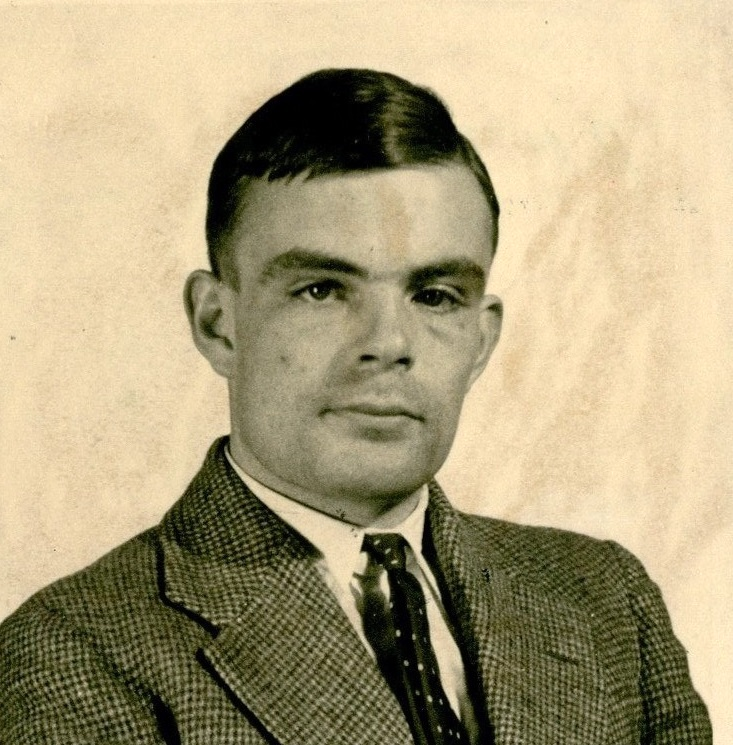
\includegraphics[width=4cm]{data/turing.jpeg}
					};
				}
				\only<2>{
					\node[inner sep=0pt, draw=black] (patient) at (5.25, -4.25) {
						
\includegraphics[width=4.5cm]{data/thinking.png}
					};

					\draw[uiored, thick] ($ (patient.east) - (0.2, 0.67) $) -- ($ (patient.east) - (1.75, 0.67) $);
				}
			}
			\only<3-4>{
				\historynode{2.35}{-0.87}{activehistory}{Dartmouth\\(1956)}{south}
				\only<3>{
					\node[inner sep=0pt] (patient) at (5.25, -4.75) {
						
\includegraphics[width=6cm]{data/dartmouth.png}
					};
				}
				\only<4>{
					\node[inner sep=0pt, align=center] (patient) at (5.25, -4.75) {
						"We propose that a 2-month, 10-man study of artificial intelligence\\
						be carried out [...]. An attempt will be made to find how to make\\
						machines use language, form abstractions and concepts, solve kinds\\
						of problems now reserved for humans, and improve themselves. We think\\
						that a significant advance can be made in [...] a summer."\\
						\textbf{- Proposal, Dartmouth summer school (1956)}
					};
				}
			}
			\only<5-6>{
				\historynode{2.68}{-1.375}{activehistory}{Perceptron\\(1958)}{north}
				\node[draw=black, inner sep=5pt, fill=white] (patient) at (2.875, -4.75) {
					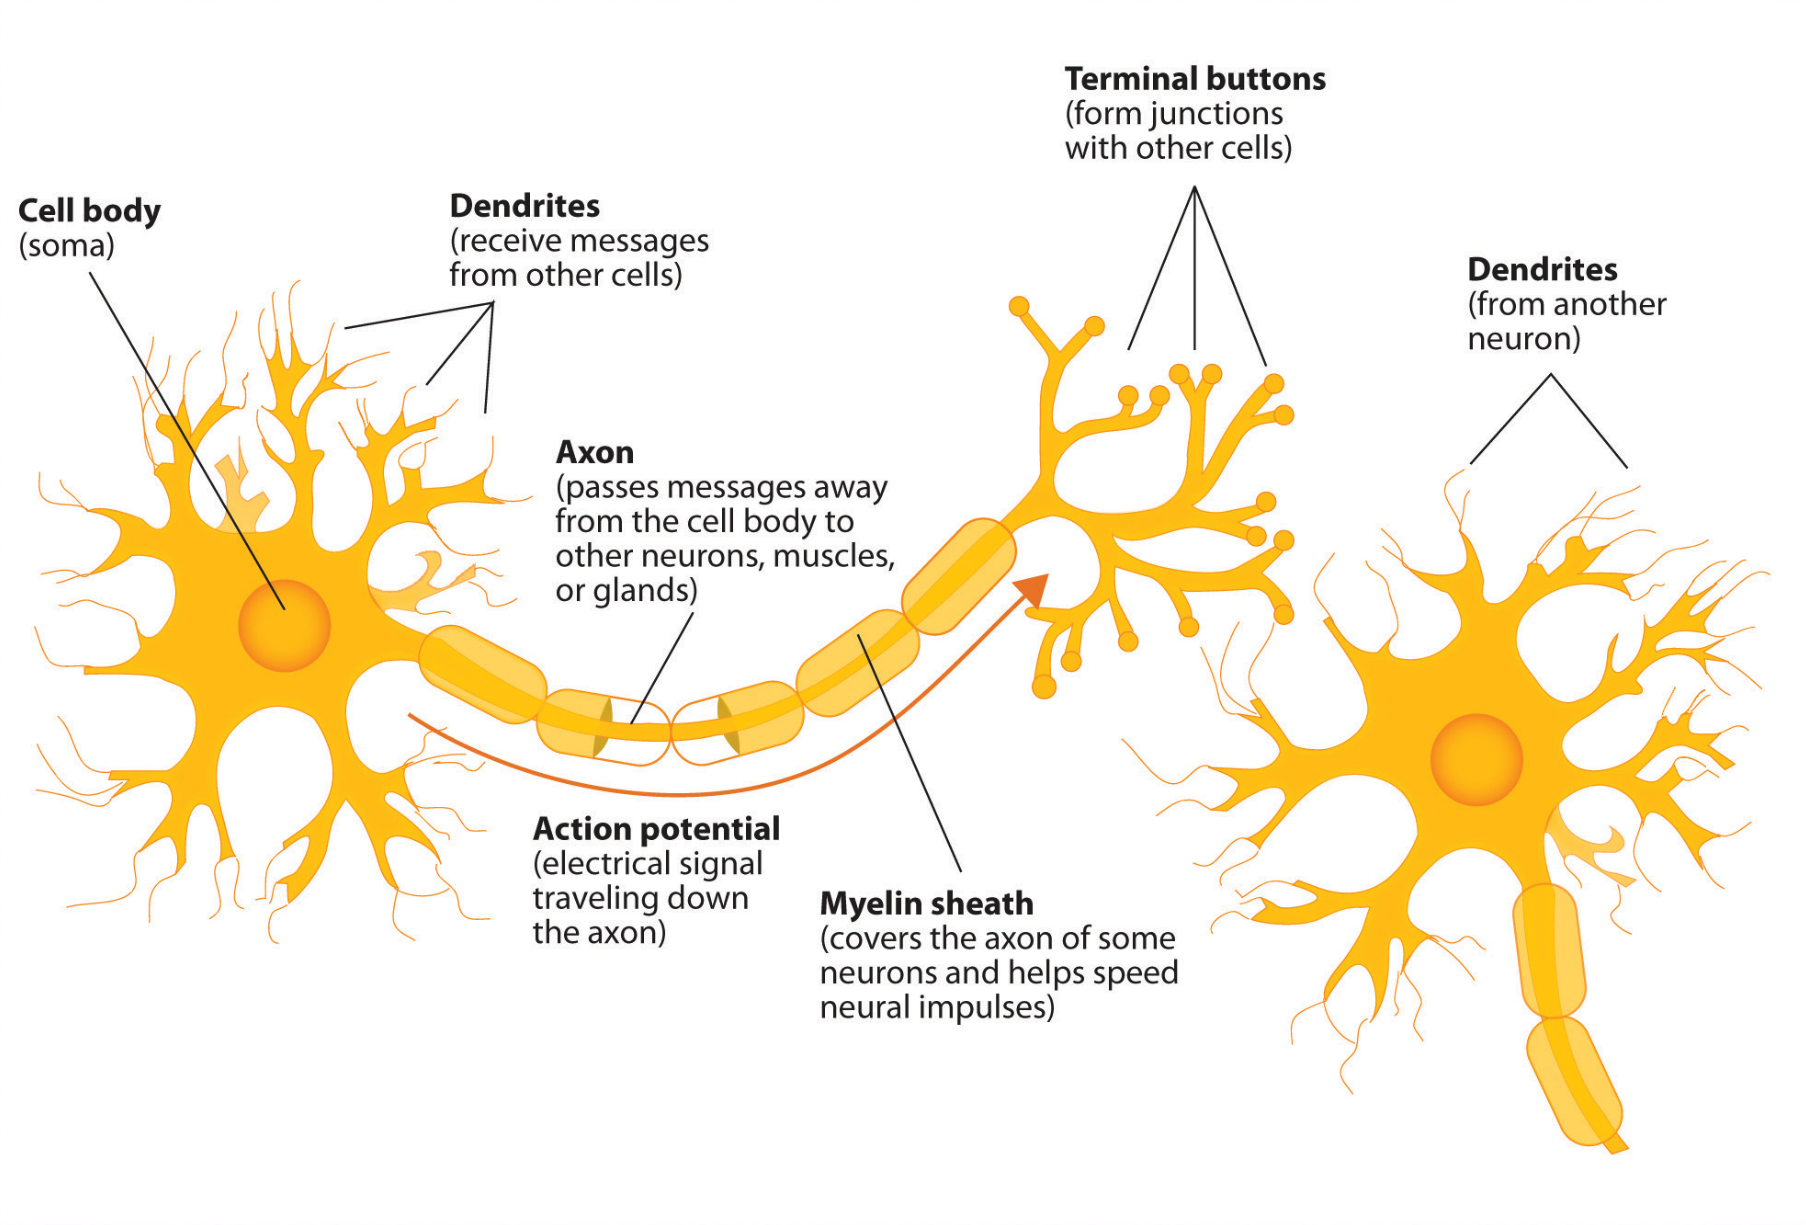
\includegraphics[width=4cm]{data/neuron.png}
				};

				\only<6>{
					\node[draw=black, inner sep=5pt, fill=white] (patient) at (2.875, -4.75) {
						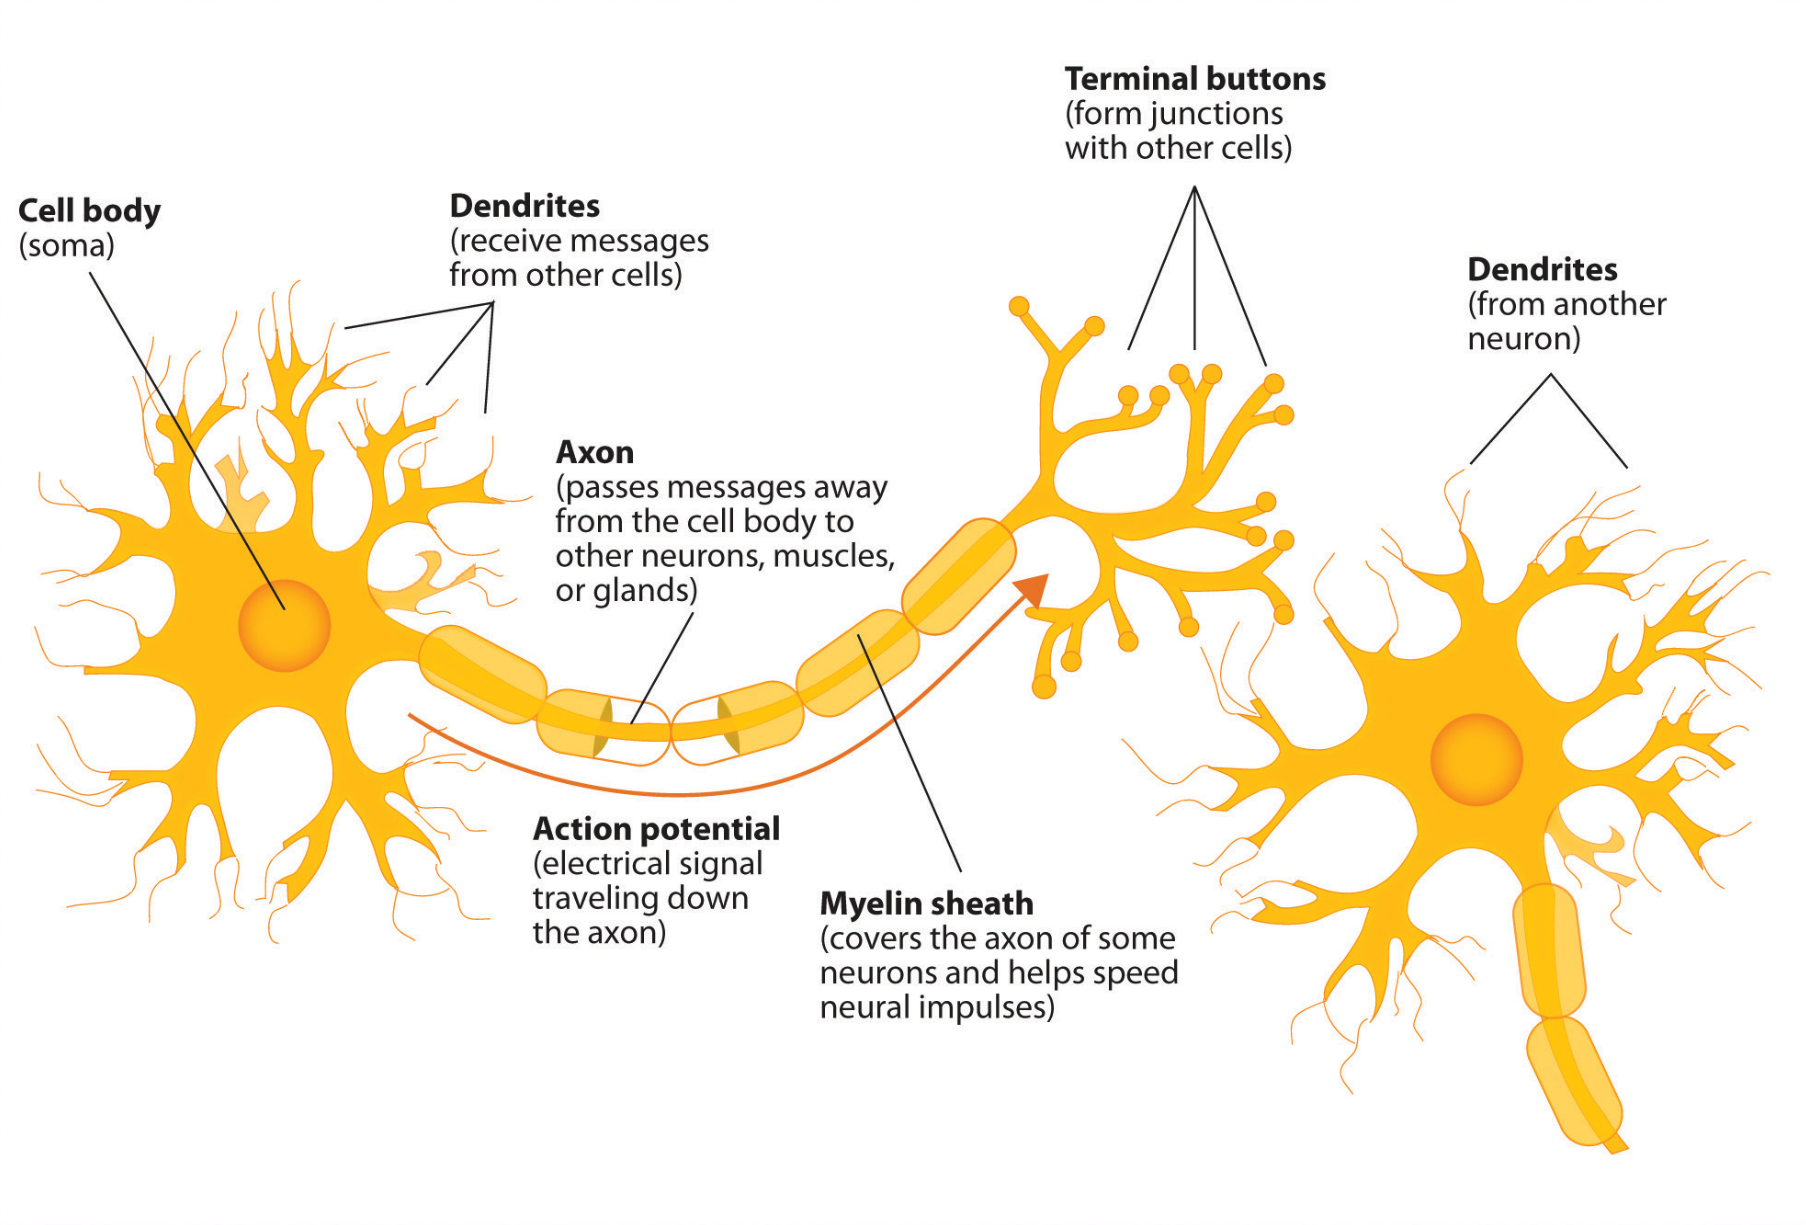
\includegraphics[width=4cm]{data/neuron.png}
					};

					\node[circle, draw=black, fill=nodefill, inner sep=2pt, text depth=0] (node) at (7.625, -4.75) {+};

					\node[] (x0) at (6.375, -3.75) {$\mathrm{input}_0$};
					\node[] (x1) at (6.375, -4.75) {$\mathrm{input}_1$};
					\node[] (x2) at (6.375, -5.75) {$\mathrm{input}_2$};

					\node[align=center] (out) at (8.875, -4.75) {$\mathrm{output}$\\$\mathrm{(0/1)}$};

					\draw[-Latex] (x0) -- (node) node [midway, above] {\small{$w_0$}};
					\draw[-Latex] (x1) -- (node) node [midway, below] {\small{$w_1$}};;
					\draw[-Latex] (x2) -- (node) node [midway, below] {\small{$w_2$}};;
					\draw[-Latex] (node) -- (out);
				}
			}
			\only<7>{
				\historynode{3.28}{-0.87}{activehistory}{Eliza\\(1964)}{south}
				\node[draw=black, inner sep=5pt, fill=white, label=below:\small{https://web.njit.edu/\~ronkowit/eliza.html}] (patient) at (5.25, -4.75) {
					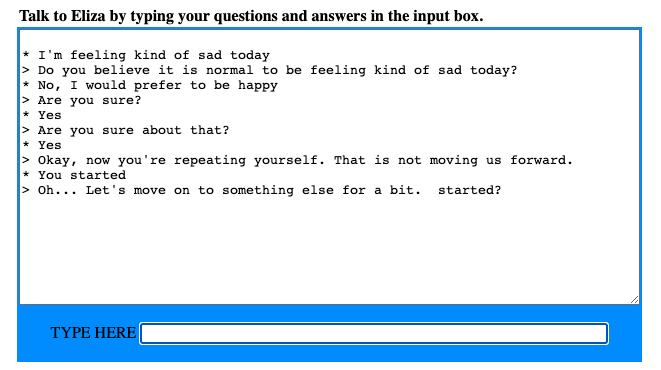
\includegraphics[width=7cm]{data/eliza.png}
				};
			}
			\only<8>{
				\historynode{5.13}{-1.375}{activehistory}{Ekspertsystemer\\(1980s)}{north}
				\node[inner sep=0pt, draw=black, label=below:\small{MYCIN (1972)}] (patient) at (5.25, -4.75) {
					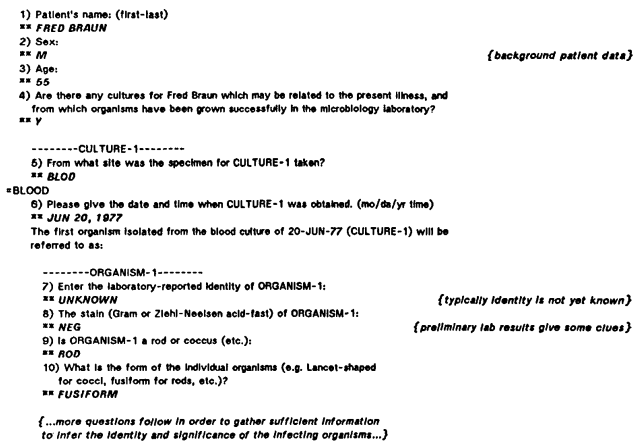
\includegraphics[width=6cm]{data/mycin.png}
				};
			}
			\only<9-10>{
				\historynode{5.82}{-0.87}{activehistory}{Nevrale nettverk\\(1986)}{south}


				\only<9>{
					\node[inner sep=0pt, minimum size=0.4cm, draw=black, circle, fill=nodefill] (n00) at (5.25, -4.75) {};

					\node[] (x0) at (4, -4) {$\mathrm{input}_0$};
					\node[] (x1) at (4, -4.75) {$\mathrm{input}_1$};
					\node[] (x2) at (4, -5.5) {$\mathrm{input}_2$};

					\node[] (out) at (6.5, -4.75) {$\mathrm{output}$};
					\draw[-] (x0.east) -- (n00);
					\draw[-] (x1.east) -- (n00);
					\draw[-] (x2.east) -- (n00);

					\draw[->] (n00) -- (out);
				}
				\only<10>{
					\node[] (x0) at (2.5, -4) {$\mathrm{input}_0$};
					\node[] (x1) at (2.5, -4.75) {$\mathrm{input}_1$};
					\node[] (x2) at (2.5, -5.5) {$\mathrm{input}_2$};

					\node[inner sep=0pt, minimum size=0.4cm, draw=black, circle, fill=nodefill] (n00) at (3.75, -3.75) {};
					\node[inner sep=0pt, minimum size=0.4cm, draw=black, circle, fill=nodefill] (n01) at (3.75, -4.25) {};
					\node[inner sep=0pt, minimum size=0.4cm, draw=black, circle, fill=nodefill] (n02) at (3.75, -4.75) {};
					\node[inner sep=0pt, minimum size=0.4cm, draw=black, circle, fill=nodefill] (n03) at (3.75, -5.25) {};
					\node[inner sep=0pt, minimum size=0.4cm, draw=black, circle, fill=nodefill] (n04) at (3.75, -5.75) {};

					\node[inner sep=0pt, minimum size=0.4cm, draw=black, circle, fill=nodefill] (n10) at (4.5, -4) {};
					\node[inner sep=0pt, minimum size=0.4cm, draw=black, circle, fill=nodefill] (n11) at (4.5, -4.5) {};
					\node[inner sep=0pt, minimum size=0.4cm, draw=black, circle, fill=nodefill] (n12) at (4.5, -5) {};
					\node[inner sep=0pt, minimum size=0.4cm, draw=black, circle, fill=nodefill] (n13) at (4.5, -5.5) {};

					\node[inner sep=0pt, minimum size=0.4cm, draw=black, circle, fill=nodefill] (n20) at (5.25, -4.25) {};
					\node[inner sep=0pt, minimum size=0.4cm, draw=black, circle, fill=nodefill] (n21) at (5.25, -4.75) {};
					\node[inner sep=0pt, minimum size=0.4cm, draw=black, circle, fill=nodefill] (n22) at (5.25, -5.25) {};

					\node[inner sep=0pt, minimum size=0.4cm, draw=black, circle, fill=nodefill] (n30) at (6, -4.5) {};
					\node[inner sep=0pt, minimum size=0.4cm, draw=black, circle, fill=nodefill] (n31) at (6, -5) {};

					\node[inner sep=0pt, minimum size=0.4cm, draw=black, circle, fill=nodefill, text depth=0] (n40) at (6.75, -4.75) {};
					\node[] (out) at (8, -4.75) {$\mathrm{output}$};

					\draw[-] (x0.east) -- (n00);
					\draw[-] (x0.east) -- (n01);
					\draw[-] (x0.east) -- (n02);
					\draw[-] (x0.east) -- (n03);
					\draw[-] (x0.east) -- (n04);
					\draw[-] (x1.east) -- (n00);
					\draw[-] (x1.east) -- (n01);
					\draw[-] (x1.east) -- (n02);
					\draw[-] (x1.east) -- (n03);
					\draw[-] (x1.east) -- (n04);
					\draw[-] (x2.east) -- (n00);
					\draw[-] (x2.east) -- (n01);
					\draw[-] (x2.east) -- (n02);
					\draw[-] (x2.east) -- (n03);
					\draw[-] (x2.east) -- (n04);

					\draw[-] (n00) -- (n10);
					\draw[-] (n00) -- (n11);
					\draw[-] (n00) -- (n12);
					\draw[-] (n00) -- (n13);
					\draw[-] (n01) -- (n10);
					\draw[-] (n01) -- (n11);
					\draw[-] (n01) -- (n12);
					\draw[-] (n01) -- (n13);
					\draw[-] (n02) -- (n10);
					\draw[-] (n02) -- (n11);
					\draw[-] (n02) -- (n12);
					\draw[-] (n02) -- (n13);
					\draw[-] (n03) -- (n10);
					\draw[-] (n03) -- (n11);
					\draw[-] (n03) -- (n12);
					\draw[-] (n03) -- (n13);
					\draw[-] (n04) -- (n10);
					\draw[-] (n04) -- (n11);
					\draw[-] (n04) -- (n12);
					\draw[-] (n04) -- (n13);

					\draw[-] (n10) -- (n20);
					\draw[-] (n10) -- (n21);
					\draw[-] (n10) -- (n22);
					\draw[-] (n11) -- (n20);
					\draw[-] (n11) -- (n21);
					\draw[-] (n11) -- (n22);
					\draw[-] (n12) -- (n20);
					\draw[-] (n12) -- (n21);
					\draw[-] (n12) -- (n22);
					\draw[-] (n13) -- (n20);
					\draw[-] (n13) -- (n21);
					\draw[-] (n13) -- (n22);

					\draw[-] (n20) -- (n30);
					\draw[-] (n20) -- (n31);
					\draw[-] (n21) -- (n30);
					\draw[-] (n21) -- (n31);
					\draw[-] (n22) -- (n30);
					\draw[-] (n22) -- (n31);

					\draw[-] (n30) -- (n40);
					\draw[-] (n31) -- (n40);

					\draw[->] (n40) -- (out);
				}
			}
			\only<11>{
				\historynode{7.10}{-1.372}{activehistory}{Deep blue\\(1997)}{north}

				\node[inner sep=0pt, draw=black, label=below:{\small{DALL-E: "A robot playing chess"}}] (img) at (2.75, -4.75) {
					
\includegraphics[width=4.3cm]{data/chess.png}
				};
				\node[anchor=north west, align=left] at ($ (img.north east)  + (0.1, 0) $) {
					\bullet\hspace{0.1cm}IBMs Deep Blue ble den første\\datamaskinen som slo sittende\\verdensmester i sjakk.\\
					\bullet\hspace{0.1cm}Deep blue vant med 3\textonehalf { }poeng mot\\Garry Kasparovs 2\textonehalf{ } etter seks spill.\\
					\bullet\hspace{0.1cm}Kasparov har uttalt at "Deep Blue\\was intelligent the way your programmable\\alarm clock is intelligent."\\
					\bullet\hspace{0.1cm}Avanserte søkealgoritmer og\\preprogrammert kunnskap fra\\sjakkeksperter.
				};
			}
			\only<12-17>{
				\historynode{8.84}{-0.87}{activehistory}{Dyplæring\\(2012)}{south}
				\only<12-13>{
					\node[inner sep=0pt, label=below:\small{Katt}] (img3) at (5.25, -4.75) {
						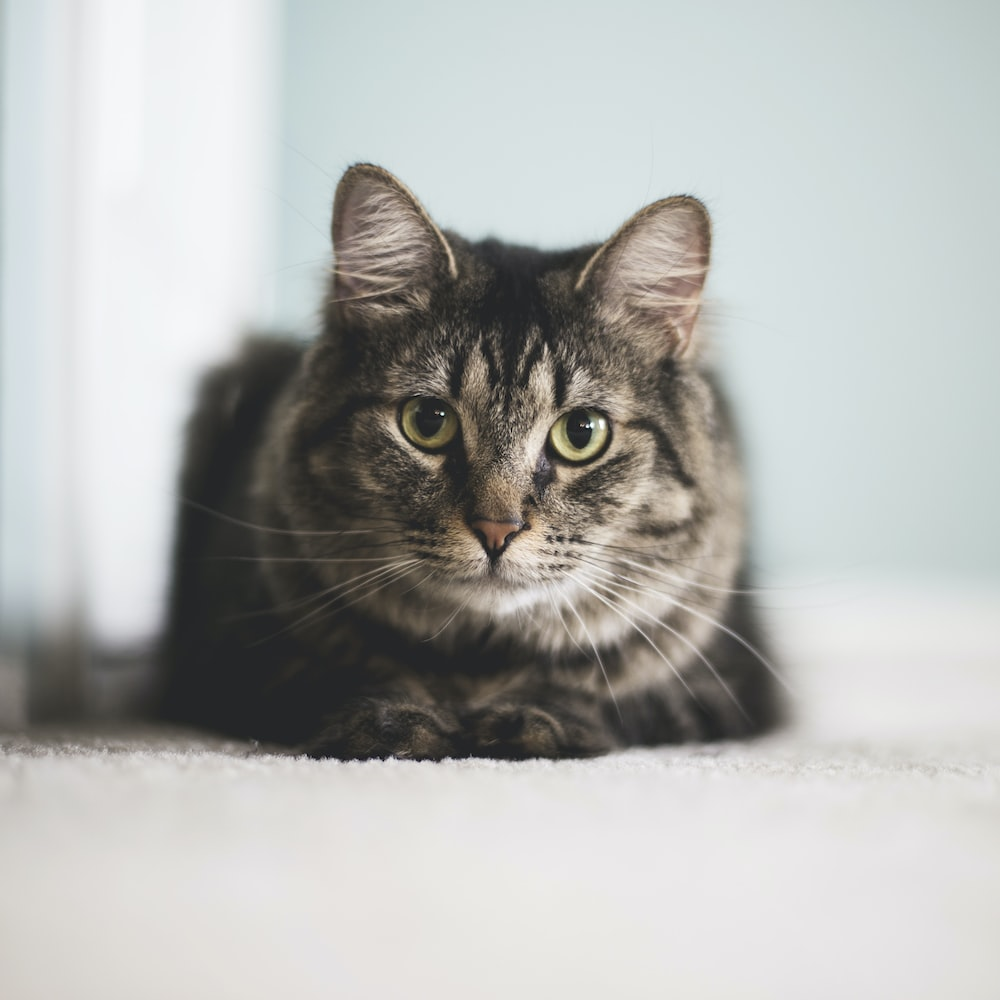
\includegraphics[width=1.5cm]{data/cat.jpeg}
					};

					\only<13>{
						\node[inner sep=0pt, label=below:\small{Fly}, anchor=west] (img4) at ($ (img3.east) + (0.1, 0) $) {
							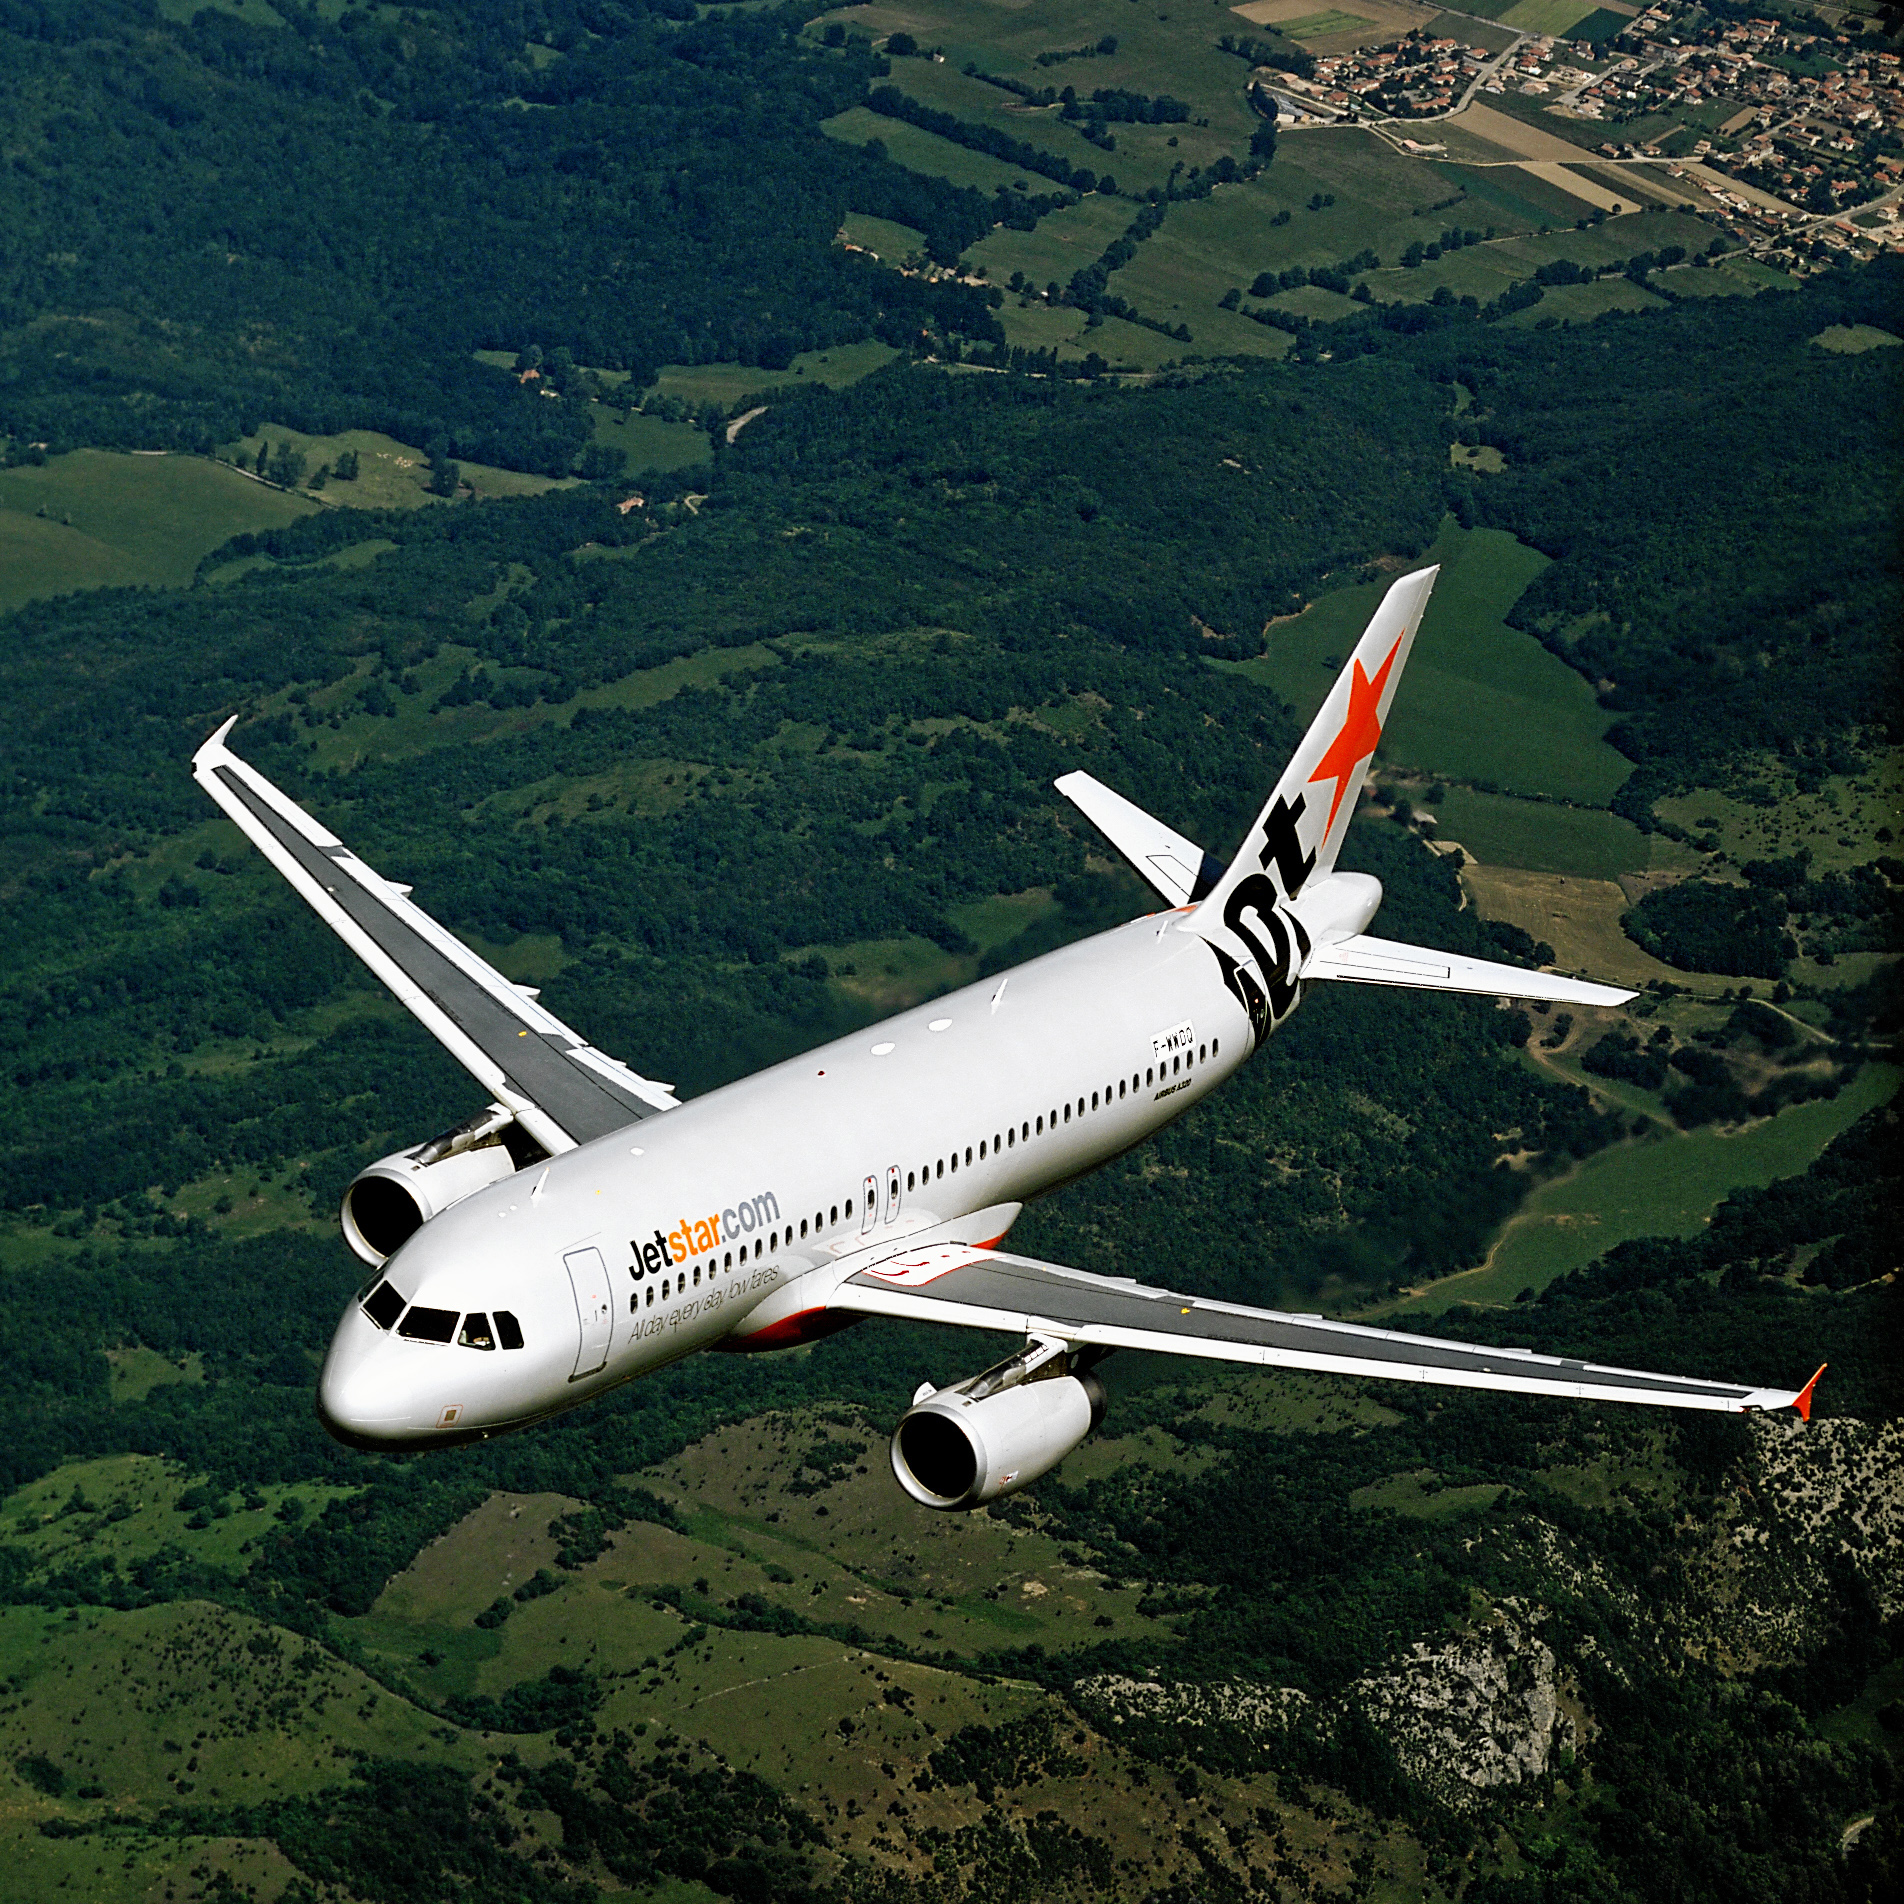
\includegraphics[width=1.5cm]{data/airplane.jpeg}
						};
						\node[inner sep=0pt, label=below:\small{Hvithai}, anchor=west] (img5) at ($ (img4.east) + (0.1, 0) $) {
							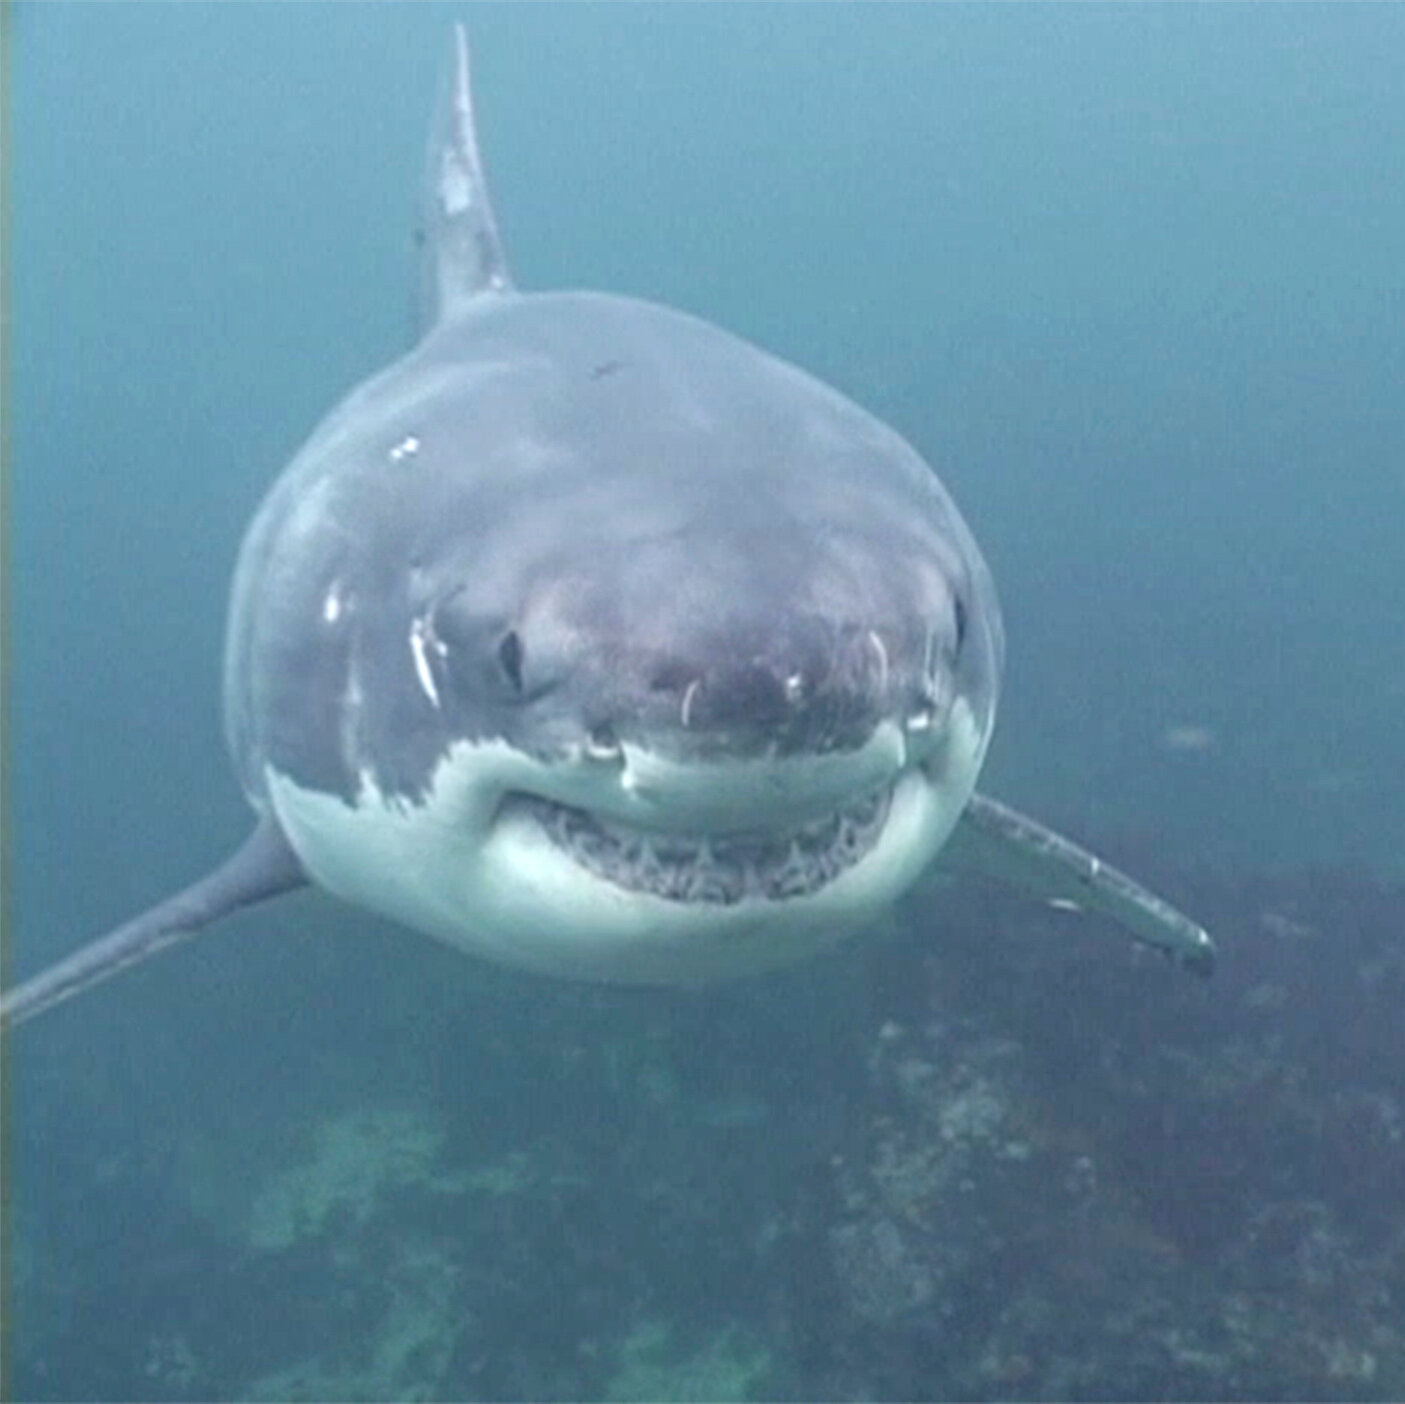
\includegraphics[width=1.5cm]{data/shark.jpeg}
						};
						\node[inner sep=0pt, label=below:\small{Marihøne}, anchor=east] (img2) at ($ (img3.west) - (0.1, 0) $) {
							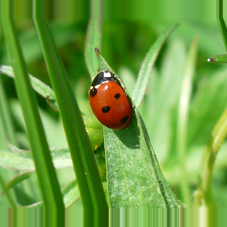
\includegraphics[width=1.5cm]{data/ladybug.png}
						};
						\node[inner sep=0pt, label=below:\small{Solsikke}, anchor=east] (img1) at ($ (img2.west) - (0.1, 0) $) {
							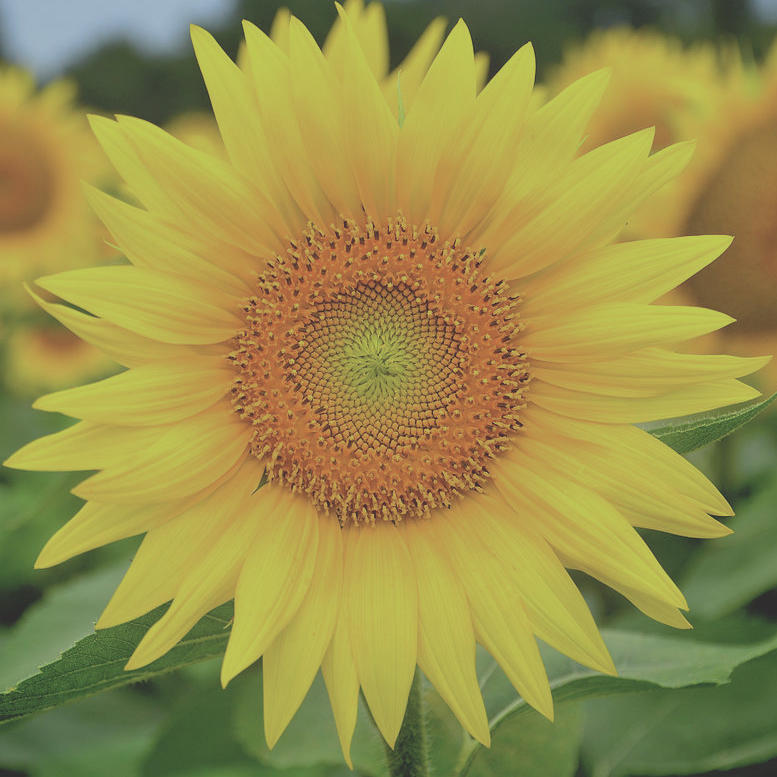
\includegraphics[width=1.5cm]{data/sunflower.jpeg}
						};
						\node[] at (5.25, -6.5) {
							ImageNet: $\sim$14m bilder fra $\sim$22k kategorier
						};
					}
				}
				\only<14>{
					\node[inner sep=0pt] at (5.25, -4.75) {
						\usebox{\imagenetold}
					};
				}
				\only<15>{
					\node[inner sep=0pt] at (5.25, -4.75) {
						\usebox{\imagenetcnn}
					};
				}
				\only<16>{
					\node[inner sep=0pt] at (5.25, -4.75) {
						\usebox{\imagenetlatest}
					};
				}
				\only<17>{
					\node[inner sep=0pt] at (5.25, -4.75) {
						\usebox{\imagenethuman}
					};
				}
			}
			\only<18>{
				\historynode{10}{-1.33}{activehistory}{ChatGPT\\(2022)}{north}
				\node[inner sep=0pt, draw=black] at (5.25, -4.75) {
					
\includegraphics[width=5cm]{data/chatgpt.png}
				};
			}
		\end{tikzpicture}
	\end{frame}

    \section{Hva er egentlig kunstig intelligens (og maskinlæring)?}

	\newcommand{\classificationplot}[1]{
		\edef\stage{#1}

		\def\xlabel{Trøtthet (t)}
		\def\ylabel{Nedstemthet (n)}
		\def\axislinestyle{black}
		\def\showticks{true}

		\ifnum\stage<3
			\renewcommand{\xlabel}{}
			\renewcommand{\ylabel}{}
			\renewcommand{\axislinestyle}{none}
			\renewcommand{\showticks}{false}
		\fi

		\begin{tikzpicture}
			\begin{axis}[
				height=5cm,
				width=5cm,
				xlabel=\xlabel,
				ylabel=\ylabel,
				axis line style={draw=\axislinestyle},
				xmajorticks=\showticks,
				ymajorticks=\showticks,
				axis x line*=bottom,
				axis y line*=left,
				xmin=-3,
				xmax=5,
				ymin=-1.5,
				ymax=4.5,
				xtick={-2, 0, 2, 4},
				xticklabels={0, 0.25, 0.5, 0.75},
				ytick={0, 2, 4},
				yticklabels={0, 0.25, 0.5}
			]	\ifnum\stage=1
					\addplot[only marks, color=gray] coordinates {
						(1.624, -1.100)
						(-0.612, -0.172)
						(-0.528, -0.878)
						(-1.073, 0.042)
						(0.865, 0.583)
						(-2.302, -1.101)
						(1.745, 1.145)
						(-0.761, 0.902)
						(0.319, 0.502)
						(-0.249, 0.901)
						(1.462, -0.684)
						(-2.060, -0.123)
						(-0.322, -0.936)
						(-0.384, -0.268)
						(1.134, 0.530)
						(1.308, 1.363)
						(1.603, 2.191)
						(1.313, 4.100)
						(1.155, 2.120)
						(1.329, 2.617)
						(1.987, 2.300)
						(0.883, 1.648)
						(2.234, 0.857)
						(3.660, 1.651)
						(2.742, 1.791)
						(1.808, 2.587)
						(1.112, 2.839)
						(1.253, 2.931)
						(3.692, 2.286)
						(2.051, 2.885)
					};
				\fi
				\ifnum\stage>1
					\addplot[only marks, color=blue!80] coordinates {
						(1.624, -1.100)
						(-0.612, -0.172)
						(-0.528, -0.878)
						(-1.073, 0.042)
						(0.865, 0.583)
						(-2.302, -1.101)
						(1.745, 1.145)
						(-0.761, 0.902)
						(0.319, 0.502)
						(-0.249, 0.901)
						(1.462, -0.684)
						(-2.060, -0.123)
						(-0.322, -0.936)
						(-0.384, -0.268)
						(1.134, 0.530)
					};
					\addplot[only marks, color=red!80] coordinates {
						(1.308, 1.363)
						(1.603, 2.191)
						(1.313, 4.100)
						(1.155, 2.120)
						(1.329, 2.617)
						(1.987, 2.300)
						(0.883, 1.648)
						(2.234, 0.857)
						(3.660, 1.651)
						(2.742, 1.791)
						(1.808, 2.587)
						(1.112, 2.839)
						(1.253, 2.931)
						(3.692, 2.286)
						(2.051, 2.885)
					};
				\fi
				\ifnum\stage=4
					\addplot[dashed, thick] coordinates {
						(-6, 3.75)
						(5, -0.5)
					};
				\fi
				\ifnum\stage=5
					\addplot[dashed, thick] coordinates {
						(-6, 3.75)
						(5, -0.5)
					};
					\node[rotate=-28] at (axis cs: -1, 2.1) {\textbf{\small{0.2$*$n+0.3$*$t}}};
				\fi
				\ifnum\stage=6
					\addplot[dashed, thick,smooth] coordinates {
						(-6, 3.25)
						(0, 1.2)
						(1.3, 1)
						(1.6, 1.5)
						(1.95, 1.45)
						(2.05, 0.6)
						(3, 0.5)
						(5, -0.5)
					};
				\fi
			\end{axis}
		\end{tikzpicture}
	}

	\newsavebox{\classificationpoints}
	\sbox{\classificationpoints}{%
		\classificationplot{1}
	}

	\newsavebox{\classificationclasses}
	\sbox{\classificationclasses}{%
		\classificationplot{2}
	}

	\newsavebox{\classificationaxes}
	\sbox{\classificationaxes}{%
		\classificationplot{3}
	}

	\newsavebox{\classificationthreshold}
	\sbox{\classificationthreshold}{%
		\classificationplot{4}
	}

	\newsavebox{\classificationmath}
	\sbox{\classificationmath}{%
		\classificationplot{5}
	}

	\newsavebox{\classificationnonlinear}
	\sbox{\classificationnonlinear}{%
		\classificationplot{6}
	}

    \begin{frame}{Hva er kunstig intelligens?} % Taxonomy, CNNs and LLMs
		\centering
		\vfill
		\begin{tikzpicture}
			\node[circle, fill=blue!60, minimum size=6cm] (ai) at (0, 0) {};
			\node[text=white, anchor=north] at ($ (ai.north) - (0, 0.3) $) {\textbf{Kunstig intelligens}};

			\onslide<2->{
				\node[text=white] at ($ (ai.north) - (-1.1, 1.2) $) {Symbolsk AI};
			}
			\onslide<13->{
				\node[circle, fill=purple!60, minimum size=4.5cm, anchor=south] (ml) at ($ (ai.south) + (0, 0.05) $) {};
				\node[text=white, anchor=north] at ($ (ml.north) - (0, 0.3) $) {\textbf{Maskinlæring}};
			}
			\onslide<25->{
				\node[text=white, align=center, font=\linespread{0.5}\selectfont] at ($ (ml.north) - (1, 1.1) $) {Lineær\\regresjon};
			}
			\onslide<26->{
				\node[circle, fill=red!60, minimum size=3cm, anchor=south] (dl) at ($ (ai.south) + (0, 0.1) $) {};
				\node[text=white, anchor=north] at ($ (dl.north) - (0, 0.3) $) {\textbf{Dyplæring}};
			}
			\onslide<36->{
				\node[align=center, text=white, font=\linespread{0.5}\selectfont] at ($ (dl.north) - (-0.2, 1.2) $) {Konvolusjonelle\\nevral nettverk};
				\node[align=center, text=white, font=\linespread{0.5}\selectfont] at ($ (dl.north) - (0.2, 2.1) $) {Store\\språkmodeller};
			}
			\only<1-2,12-13,24-26,35-36>{
				\only<1>{
					\node[anchor=north west, align=left, font=\small] (ai-text) at ($ (ai.north) + (3.5, 0.0) $) {\textbf{Kunstig intelligens (AI):}\\Maskiner som løser problemer\\som krever intelligens};
				}
				\onslide<2->{
					\node[anchor=north west, align=left, font=\small, text=gray!40] (ai-text) at ($ (ai.north) + (3.5, 0.0) $) {\textbf{Kunstig intelligens (AI):}\\Maskiner som løser problemer\\som krever intelligens};
				}
				\only<12>{
					\node[anchor=north west, align=left, font=\small] (ml-text) at ($ (ai-text.south west) - (0, 0) $) {\textbf{Symbolsk AI:}\\Tradisjonell AI der problemer\\løses gjennom oppslag mot regler,\\gjerne definert av menneskelige\\eksperter};
				}
				\only<13,24>{
					\node[anchor=north west, align=left, font=\small] (ml-text) at ($ (ai-text.south west) - (0, 0) $) {\textbf{Maskinlæring:}\\Maskiner som lærer å løse problemer\\gjennom å finne mønster i data på\\egenhånd};
				}
				\onslide<25->{
				 	\node[anchor=north west, align=left, font=\small, text=gray!40] (ml-text) at ($ (ai-text.south west) - (0, 0) $) {\textbf{Maskinlæring (ML):}\\Maskiner som lærer å løse problemer\\gjennom å finne mønster i data på\\egenhånd};
				}
				\only<25>{
					\node[anchor=north west, align=left, font=\small] (dl-text) at ($ (ml-text.south west) - (0, 0) $) {\textbf{Lineær regresion:}\\Maskinlæringsmodeller som \\finner lineære (m.a.o. enkle) mønstre};
				}
				\only<26,35>{
					\node[anchor=north west, align=left, font=\small] (dl-text) at ($ (ml-text.south west) - (0, 0) $) {\textbf{Dyplæring:}\\Maskinlæringsmodeller som er\\hierarkisk organisert ($\approx$ dype\\nevrale nettverk), inspirert av\\hjernens struktur};
				}
				\onslide<36->{
					\node[anchor=north west, align=left, font=\small, text=gray!40] (dl-text) at ($ (ml-text.south west) - (0, 0) $) {\textbf{Dyplæring:}\\Maskinlæringsmodeller som er\\hierarkisk organisert ($\approx$ dype\\nevrale nettverk), inspirert av\\hjernens struktur};
				}
				\only<36>{
					\node[anchor=north west, align=left, font=\small] (cnn-text) at ($ (dl-text.south west) - (0, 0) $) {\textbf{Konvolusjonelle nevrale nettverk:}\\Nevrale nettverk for prosessering\\av bildedata};
					\node[anchor=north west, align=left, font=\small] at ($ (cnn-text.south west) - (0, 0) $) {\textbf{Store språkmodeller:}\\(Store) nevrale nettverk\\for språkprosessering (f.eks. ChatGPT)};
				}
			}

			\def\outerwidth{2pt}
			\def\outercolour{gray!80}
			\def\offset{0.6}
			\colorlet{systemcolour}{gray!10}
			\colorlet{rulescolour}{blue!20}
			\colorlet{rulecolour}{cyan!20}

			\only<3-11>{
				\node[
					minimum width=3.8cm,
					minimum height=2.8cm,
					draw=black,
					fill=systemcolour,
					label=above:{\textbf{\small{PSYCIN}}}
				] (system) at (5.5, -1) {};

				\onslide<4->{
					\node[] (doctor) at (5.5, 2.5) {
						\Huge{\emoji{woman-health-worker}}
					};
				}
				\onslide<5->{
					\node[] (notes) at (5.5 - \offset, 1.25) {
						\Huge{\emoji{spiral-notepad}}
					};
					\draw[-stealth, line width=\outerwidth, \outercolour]
						(doctor) to [out=270, in=90]
						(notes) --
						($ (system.north) - (\offset, 0) $);
				}

				\onslide<6->{
					\node[
						minimum width=2.4cm,
						minimum height=1.6cm,
						draw=black,
						fill=rulescolour,
						label=above:{\textbf{\footnotesize{Regelmotor}}}
					] (rules) at ($ (system) - (0, 0.5) $) {};
					\draw[-stealth, line width=\outerwidth, \outercolour]
						($ (system.north) - (\offset, 0) $) to [in=0, out=270]
						($ (rules.north west) + (-0.2, 0.2) $) to [in=180, out=180]
						($ (rules.west) - (0.2, 0) $) --
						(rules.west);
				}
				\onslide<7->{
					\node[
						minimum width=1.5cm,
						minimum height=0.3cm,
						draw=black,
						fill=rulecolour
					] (rule1) at ($ (rules) + (0, 0.5) $) {
						\small{Nedstemt}
					};
					\node[
						minimum width=1.5cm,
						minimum height=0.3cm,
						draw=black,
						fill=rulecolour
					] (rule2) at ($ (rules) + (0, 0.0) $) {
						\small{Søvnløshet}
					};
					\node[
						minimum width=1.5cm,
						minimum height=0.3cm,
						draw=black,
						fill=rulecolour
					] (rule3) at ($ (rules) + (0, -0.5) $) {
						\small{Tretthet}
					};
					\draw[] (rules.west) to [in=180, out=0] (rule1.west);
					\draw[] (rules.west) to [in=180, out=0] (rule2.west);
					\draw[] (rules.west) to [in=180, out=0] (rule3.west);

					\draw[] (rule1.east) to [in=180, out=0] (rules.east);
					\draw[] (rule2.east) to [in=180, out=0] (rules.east);
					\draw[] (rule3.east) to [in=180, out=0] (rules.east);
				}

				\onslide<8->{
					\draw[-stealth, line width=\outerwidth, \outercolour]
						(rules.east) --
						($ (rules.east) + (0.2, 0) $) to [out=0, in=0]
						($ (rules.north east) + (0.2, 0.2) $) to [out=180, in=270]
						($ (system.north) + (\offset, 0) $);

					\node[minimum height=0.75cm] (diagnosis) at (5.5 + \offset, 1.25) {
						\small{Depresjon}
					};

					\draw[line width=\outerwidth, \outercolour]
						($ (system.north) + (\offset, 0) $) --
						(diagnosis) to [out=90, in=270]
						(doctor);
				}
				\only<9>{
					\draw[red, thick] (system.north east) -- (system.north west) -- (system.south west) -- (system.south east) -- cycle;
					\draw[red, thick] (rules.north east) -- (rules.north west) -- (rules.south west) -- (rules.south east) -- cycle;
				}
				\onslide<10->{
					\draw[red!20, thick] (system.north east) -- (system.north west) -- (system.south west) -- (system.south east) -- cycle;
					\draw[red!20, thick] (rules.north east) -- (rules.north west) -- (rules.south west) -- (rules.south east) -- cycle;
				}
				\only<10>{
					\draw[red, thick] (notes.north east) -- (notes.north west) -- (notes.south west) -- (notes.south east) -- cycle;
				}
				\onslide<11->{
					\draw[red!20, thick] (notes.north east) -- (notes.north west) -- (notes.south west) -- (notes.south east) -- cycle;
				}
				\only<11>{
					\node[] (scientist) at ($ (system.south) - (0, 1) $) {
						\Huge{\emoji{man-scientist}}
					};

					\draw[red, thick] (rule1.north east) -- (rule1.north west) -- (rule1.south west) -- (rule1.south east) -- cycle;
					\draw[red, thick] (rule2.north east) -- (rule2.north west) -- (rule2.south west) -- (rule2.south east) -- cycle;
					\draw[red, thick] (rule3.north east) -- (rule3.north west) -- (rule3.south west) -- (rule3.south east) -- cycle;
					\draw[-stealth, red, thick, dashed] (scientist) -- (rule3);
				}
			}

			\only<14-23>{
				\only<14,23>{
					\node[
						minimum width=3.8cm,
						minimum height=2.8cm,
						draw=black,
						fill=systemcolour,
						label=above:{\textbf{\small{PSYCIN}}}
					] (system) at (5.5, -1) {};

					\node[] (doctor) at (5.5, 2.5) {
						\Huge{\emoji{woman-health-worker}}
					};

					\node[] (notes) at (5.5 - \offset, 1.25) {
						\Huge{\emoji{spiral-notepad}}
					};
					\draw[-stealth, line width=\outerwidth, \outercolour]
						(doctor) to [out=270, in=90]
						(notes) --
						($ (system.north) - (\offset, 0) $);
				}

				\only<14-16,22-23>{
					\node[
						minimum width=2.4cm,
						minimum height=1.6cm,
						draw=black,
						fill=rulescolour,
						label=above:{\textbf{\footnotesize{Regelmotor}}}
					] (rules) at (5.5, -1.5) {};
				}

				\only<14,23>{
					\draw[-stealth, line width=\outerwidth, \outercolour]
						($ (system.north) - (\offset, 0) $) to [in=0, out=270]
						($ (rules.north west) + (-0.2, 0.2) $) to [in=180, out=180]
						($ (rules.west) - (0.2, 0) $) --
						(rules.west);
				}

				\only<14-15>{
					\node[
						minimum width=1.5cm,
						minimum height=0.3cm,
						draw=black,
						fill=rulecolour
					] (rule1) at ($ (rules) + (0, 0.5) $) {
						\small{Nedstemt}
					};
					\node[
						minimum width=1.5cm,
						minimum height=0.3cm,
						draw=black,
						fill=rulecolour
					] (rule2) at ($ (rules) + (0, 0.0) $) {
						\small{Søvnløshet}
					};
					\node[
						minimum width=1.5cm,
						minimum height=0.3cm,
						draw=black,
						fill=rulecolour
					] (rule3) at ($ (rules) + (0, -0.5) $) {
						\small{Tretthet}
					};
					\draw[] (rules.west) to [in=180, out=0] (rule1.west);
					\draw[] (rules.west) to [in=180, out=0] (rule2.west);
					\draw[] (rules.west) to [in=180, out=0] (rule3.west);

					\draw[] (rule1.east) to [in=180, out=0] (rules.east);
					\draw[] (rule2.east) to [in=180, out=0] (rules.east);
					\draw[] (rule3.east) to [in=180, out=0] (rules.east);
				}

				\only<14,23>{
					\draw[-stealth, line width=\outerwidth, \outercolour]
						(rules.east) --
						($ (rules.east) + (0.2, 0) $) to [out=0, in=0]
						($ (rules.north east) + (0.2, 0.2) $) to [out=180, in=270]
						($ (system.north) + (\offset, 0) $);

					\node[minimum height=0.75cm] (diagnosis) at (5.5 + \offset, 1.25) {
						\small{Depresjon}
					};

					\draw[line width=\outerwidth, \outercolour]
						($ (system.north) + (\offset, 0) $) --
						(diagnosis) to [out=90, in=270]
						(doctor);
				}

				\only<17>{
					\node[anchor=north east] at (8.25, 1) {
						\usebox{\classificationpoints}
					};
				}
				\only<18>{
					\node[anchor=north east] at (8.25, 1) {
						\usebox{\classificationclasses}
					};
				}
				\only<19>{
					\node[anchor=north east] at (8.25, 1) {
						\usebox{\classificationaxes}
					};
				}
				\only<20>{
					\node[anchor=north east] at (8.25, 1) {
						\usebox{\classificationthreshold}
					};
				}
				\only<21>{
					\node[anchor=north east] at (8.25, 1) {
						\usebox{\classificationmath}
					};
				}
				\only<22-23>{
					\node[] at (rules) {
						\small{0.2*n+0.3*t}
					};
				}
			}

			\only<27-34>{
				\only<32-34>{
					\node[
						minimum width=3.8cm,
						minimum height=2.8cm,
						draw=black,
						fill=systemcolour,
						label=above:{\textbf{\small{PSYCIN}}}
					] (system) at (5.5, -1) {};

					\node[] (doctor) at (5.5, 2.5) {
						\Huge{\emoji{woman-health-worker}}
					};

					\only<32-33>{
						\node[] (notes) at (5.5 - \offset, 1.25) {
							\Huge{\emoji{spiral-notepad}}
						};
						\draw[-stealth, line width=\outerwidth, \outercolour]
							(doctor) to [out=270, in=90]
							(notes) --
							($ (system.north) - (\offset, 0) $);
					}
				}

				\only<27-29,32-34>{
					\node[
						minimum width=2.4cm,
						minimum height=1.6cm,
						draw=black,
						fill=rulescolour,
						label=above:{\textbf{\footnotesize{Regelmotor}}}
					] (rules) at (5.5, -1.5) {};
				}
				\only<27>{
					\node[] at (rules) {
						\small{0.2*n+0.3*t}
					};
				}
				\only<28,32-34>{
					\def\nodesize{8pt}
					\def\vsep{0.35}
					\def\hsep{0.7}
					\def\arrowstyle{-}

					\node[circle, minimum size=\nodesize, draw=black, fill=rulecolour, inner sep=0pt] (n11) at (rules) {};
					\node[circle, minimum size=\nodesize, draw=black, fill=rulecolour, inner sep=0pt] (n10) at ($ (n11) + (0, \vsep) $) {};
					\node[circle, minimum size=\nodesize, draw=black, fill=rulecolour, inner sep=0pt] (n12) at ($ (n11) + (0, -\vsep) $) {};

					\node[circle, minimum size=\nodesize, draw=black, fill=rulecolour, inner sep=0pt] (n00) at ($ (n11) - (\hsep, -1.5 * \vsep) $) {};
					\node[circle, minimum size=\nodesize, draw=black, fill=rulecolour, inner sep=0pt] (n01) at ($ (n11) - (\hsep, -0.5 * \vsep) $) {};
					\node[circle, minimum size=\nodesize, draw=black, fill=rulecolour, inner sep=0pt] (n02) at ($ (n11) - (\hsep, 0.5 * \vsep) $) {};
					\node[circle, minimum size=\nodesize, draw=black, fill=rulecolour, inner sep=0pt] (n03) at ($ (n11) - (\hsep, 1.5 * \vsep) $) {};

					\node[circle, minimum size=\nodesize, draw=black, fill=rulecolour, inner sep=0pt] (n20) at ($ (n11) + (\hsep, 0.5 * \vsep) $) {};
					\node[circle, minimum size=\nodesize, draw=black, fill=rulecolour, inner sep=0pt] (n21) at ($ (n11) + (\hsep, -0.5 * \vsep) $) {};

					\draw[\arrowstyle] (rules.west) to [in=180, out=0] (n00);
					\draw[\arrowstyle] (rules.west) to [in=180, out=0] (n01);
					\draw[\arrowstyle] (rules.west) to [in=180, out=0] (n02);
					\draw[\arrowstyle] (rules.west) to [in=180, out=0] (n03);

					\draw[\arrowstyle] (n00) to [in=180, out=0] (n10);
					\draw[\arrowstyle] (n00) to [in=180, out=0] (n11);
					\draw[\arrowstyle] (n00) to [in=180, out=0] (n12);
					\draw[\arrowstyle] (n01) to [in=180, out=0] (n10);
					\draw[\arrowstyle] (n01) to [in=180, out=0] (n11);
					\draw[\arrowstyle] (n01) to [in=180, out=0] (n12);
					\draw[\arrowstyle] (n02) to [in=180, out=0] (n10);
					\draw[\arrowstyle] (n02) to [in=180, out=0] (n11);
					\draw[\arrowstyle] (n02) to [in=180, out=0] (n12);
					\draw[\arrowstyle] (n03) to [in=180, out=0] (n10);
					\draw[\arrowstyle] (n03) to [in=180, out=0] (n11);
					\draw[\arrowstyle] (n03) to [in=180, out=0] (n12);

					\draw[\arrowstyle] (n10) to [in=180, out=0] (n20);
					\draw[\arrowstyle] (n10) to [in=180, out=0] (n21);
					\draw[\arrowstyle] (n11) to [in=180, out=0] (n20);
					\draw[\arrowstyle] (n11) to [in=180, out=0] (n21);
					\draw[\arrowstyle] (n12) to [in=180, out=0] (n20);
					\draw[\arrowstyle] (n12) to [in=180, out=0] (n21);

					\draw[\arrowstyle] (n20) to [in=180, out=0] (rules.east);
					\draw[\arrowstyle] (n21) to [in=180, out=0] (rules.east);
				}
				\only<29>{
					\node[align=left] at (rules) {
						\small{0.2$*$n+0.3$*$t-0.1$*$(t-1)$*$}\\
						\small{0.5$*$(n-0.4$*$t-0.1$*$t)$*$}\\
						\small{0.2-(0.4$*$n-0.5$*$t-n)}
					};
				}
				\only<30>{
					\node[] at (5.5, -1) {
						\usebox{\classificationthreshold}
					};
				}
				\only<31>{
					\node[] at (5.5, -1) {
						\usebox{\classificationnonlinear}
					};
				}

				\only<32-34>{
					\draw[-stealth, line width=\outerwidth, \outercolour]
						($ (system.north) - (\offset, 0) $) to [in=0, out=270]
						($ (rules.north west) + (-0.2, 0.2) $) to [in=180, out=180]
						($ (rules.west) - (0.2, 0) $) --
						(rules.west);

					\draw[-stealth, line width=\outerwidth, \outercolour]
						(rules.east) --
						($ (rules.east) + (0.2, 0) $) to [out=0, in=0]
						($ (rules.north east) + (0.2, 0.2) $) to [out=180, in=270]
						($ (system.north) + (\offset, 0) $);

					\node[minimum height=0.75cm] (diagnosis) at (5.5 + \offset, 1.25) {
						\small{Depresjon}
					};

					\draw[line width=\outerwidth, \outercolour]
						($ (system.north) + (\offset, 0) $) --
						(diagnosis) to [out=90, in=270]
						(doctor);
				}
				\only<33-34>{
					\node[] (patient) at (4, 2.5) {
						\Huge{\emoji{pensive-face}}
					};
					\draw[stealth-stealth, line width=\outerwidth, \outercolour]
						(patient) -- (doctor);
					\only<34>{
						\draw[-stealth, line width=\outerwidth, \outercolour]
						(patient.south) to [out=270, in=90] ($ (system.north) - (\offset, 0) $);
					}
				}
			}

			%\node[anchor=north west, align=left, font=\small, text=gray!40] (dl-text) at ($ (ml-text.south west) - (0, 0) $) {\textbf{Dyplæring:}\\Maskinlæringsmodeller som er\\hierarkisk organisert ($\approx$ dype\\nevrale nettverk), inspirert av\\hjernens struktur};
			%\node[anchor=north west, align=left, font=\small] (cnn-text) at ($ (dl-text.south west) - (0, 0) $) {\textbf{Konvolusjonelle nevrale nettverk:}\\Nevrale nettverk for prosessering\\av bildedata};
			%\node[anchor=north west, align=left, font=\small] at ($ (cnn-text.south west) - (0, 0) $) {\textbf{Store språkmodeller:}\\(Store) nevrale nettverk\\for språkprosessering (ChatGPT)};
			\node[] at (-3, 3) {};
			\node[] at (7.7, -4) {};
		\end{tikzpicture}
		\vfill
	\end{frame}

    \section{Kunstig intelligens i hjerneforskning}

	\begin{frame}{AI i hjerneforskning}
		\centering
		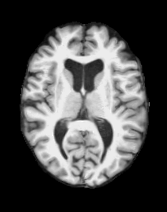
\includegraphics[width=3cm]{data/samples/control_0.png}
	\end{frame}

	\begin{frame}{AI i hjerneforskning} % Lacking data
        \vfill
		\begin{tikzpicture}
            \newcommand{\mrivsep}{0.52}
			\newcommand{\mrihsep}{0.44}
			\def\plotwidth{11.68}

			\newcommand{\nodesize}{11pt}
			\newcommand{\hsep}{28pt}
			\newcommand{\vsep}{14pt}

			\newcommand{\arrowwidth}{0.05cm}
			\newcommand{\innerarrow}{{Latex[length=0.1cm, width=0.15cm]}}
			\newcommand{\outerarrow}{{Latex[length=0.2cm, width=0.3cm]}}

			\definecolor{cb-green}{HTML}{4dac93}
			\definecolor{cb-blue}{HTML}{3594d6}
			\definecolor{outercolor}{RGB}{128, 128, 128}
			\colorlet{train-fill}{cb-blue}

			\newcommand{\patientlocation}[1]{($ (1, -1.6) + ####1 $)}
			\newcommand{\controllocation}[1]{($ (1, -2.8) + ####1 $)}
			\newcommand{\modellocation}[1]{($ (0.5 * \plotwidth, -2.2) + ####1 $)}

            \node[thick, draw=green, inner sep=0pt] (p0) at (2, -1.1) {
                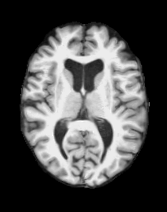
\includegraphics[width=0.6cm]{data/samples/control_0.png}
            };

            \node[thick, draw=green, inner sep=0pt] (p0) at (1.1, -0.7) {
                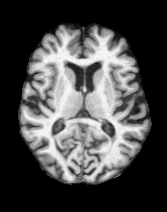
\includegraphics[width=0.6cm]{data/samples/control_1.png}
            };

            \node[thick, draw=green, inner sep=0pt] (p0) at (1.25, -1.9) {
                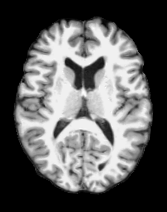
\includegraphics[width=0.6cm]{data/samples/control_2.png}
            };

            \node[thick, draw=green, inner sep=0pt] (p0) at (0.3, -1.4) {
                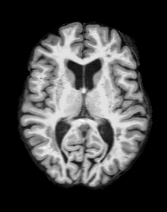
\includegraphics[width=0.6cm]{data/samples/control_3.png}
            };

            \node[thick, draw=red, inner sep=0pt] (p0) at (2.2, -3.1) {
                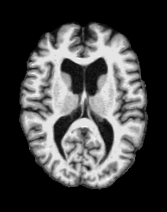
\includegraphics[width=0.6cm]{data/samples/control_4.png}
            };

            \node[thick, draw=red, inner sep=0pt] (p0) at (1.4, -3.2) {
                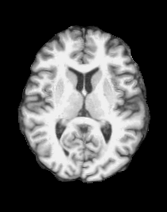
\includegraphics[width=0.6cm]{data/samples/control_5.png}
            };

            \node[thick, draw=red, inner sep=0pt] (p0) at (0.4, -2.7) {
                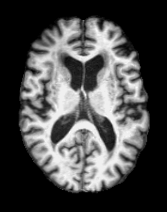
\includegraphics[width=0.6cm]{data/samples/dementia_0.png}
            };

			\only<2>{
			\node[circle, inner sep=0pt, fill=none, outer sep=0pt, line width=0pt, draw=none] (n00) at \modellocation{(-3 * \hsep, 0)} {};

			\node[circle, minimum size=\nodesize, inner sep=0pt, fill=train-fill!35, outer sep=0pt, line width=0pt, draw=train-fill!35] (n10) at \modellocation{(-2 * \hsep, 2 * \vsep)} {};
			\node[circle, minimum size=\nodesize, inner sep=0pt, fill=train-fill, outer sep=0pt, line width=0pt, draw=train-fill] (n11) at \modellocation{(-2 * \hsep, 1 * \vsep)} {};
			\node[circle, minimum size=\nodesize, inner sep=0pt, fill=train-fill!15, outer sep=0pt, line width=0pt, draw=train-fill!15] (n12) at \modellocation{(-2 * \hsep, 0)} {};
			\node[circle, minimum size=\nodesize, inner sep=0pt, fill=train-fill!85, outer sep=0pt, line width=0pt, draw=train-fill!85] (n13) at \modellocation{(-2 * \hsep, -1 * \vsep)} {};
			\node[circle, minimum size=\nodesize, inner sep=0pt, fill=train-fill!90, outer sep=0pt, line width=0pt, draw=train-fill!90] (n14) at \modellocation{(-2 * \hsep, -2 * \vsep)} {};

			\node[circle, minimum size=\nodesize, inner sep=0pt, fill=train-fill!55, outer sep=0pt, line width=0pt, draw=train-fill!55] (n20) at \modellocation{(-1 * \hsep, 1.5 * \vsep)} {};
			\node[circle, minimum size=\nodesize, inner sep=0pt, fill=train-fill!20, outer sep=0pt, line width=0pt, draw=train-fill!20] (n21) at \modellocation{(-1 * \hsep, 0.5 * \vsep)} {};
			\node[circle, minimum size=\nodesize, inner sep=0pt, fill=train-fill!90, outer sep=0pt, line width=0pt, draw=train-fill!50] (n22) at \modellocation{(-1 * \hsep, -0.5 * \vsep)} {};
			\node[circle, minimum size=\nodesize, inner sep=0pt, fill=train-fill!35, outer sep=0pt, line width=0pt, draw=train-fill!35] (n23) at \modellocation{(-1 * \hsep, -1.5 * \vsep)} {};

			\node[circle, minimum size=\nodesize, inner sep=0pt, fill=train-fill!95, outer sep=0pt, line width=0pt, draw=train-fill!65] (n30) at \modellocation{(0 * \hsep, 1.5 * \vsep)} {};
			\node[circle, minimum size=\nodesize, inner sep=0pt, fill=train-fill!20, outer sep=0pt, line width=0pt, draw=train-fill!20] (n31) at \modellocation{(0 * \hsep, 0.5 * \vsep)} {};
			\node[circle, minimum size=\nodesize, inner sep=0pt, fill=train-fill!90, outer sep=0pt, line width=0pt, draw=train-fill!90] (n32) at \modellocation{(0 * \hsep, -0.5 * \vsep)} {};
			\node[circle, minimum size=\nodesize, inner sep=0pt, fill=train-fill!80, outer sep=0pt, line width=0pt, draw=train-fill!80] (n33) at \modellocation{(0 * \hsep, -1.5 * \vsep)} {};

			\node[circle, minimum size=\nodesize, inner sep=0pt, fill=train-fill!50, outer sep=0pt, line width=0pt, draw=train-fill!50] (n40) at \modellocation{(1 * \hsep, 1*\vsep)} {};
			\node[circle, minimum size=\nodesize, inner sep=0pt, fill=train-fill!90, outer sep=0pt, line width=0pt, draw=train-fill!70] (n41) at \modellocation{(1 * \hsep, 0*\vsep)} {};
			\node[circle, minimum size=\nodesize, inner sep=0pt, fill=train-fill!70, outer sep=0pt, line width=0pt, draw=train-fill!30] (n42) at \modellocation{(1 * \hsep, -1*\vsep)} {};

			\node[circle, minimum size=\nodesize, inner sep=0pt, fill=train-fill, outer sep=0pt, line width=0pt, draw=train-fill] (n50) at \modellocation{(2 * \hsep, 1*\vsep)} {};
			\node[circle, minimum size=\nodesize, inner sep=0pt, fill=train-fill!70, outer sep=0pt, line width=0pt, draw=train-fill!70] (n51) at \modellocation{(2 * \hsep, 0*\vsep)} {};
			\node[circle, minimum size=\nodesize, inner sep=0pt, fill=train-fill!30, outer sep=0pt, line width=0pt, draw=train-fill!30] (n52) at \modellocation{(2 * \hsep, -1*\vsep)} {};

			\node[circle, minimum size=\nodesize, inner sep=0pt, fill=train-fill!80, outer sep=0pt, line width=0pt, draw=train-fill!65] (n60) at \modellocation{(3 * \hsep, 0)} {};

			\draw[
				color=train-fill!35,
				-\innerarrow,
				line width=\arrowwidth
			] (n00) to [out=20,in=200] (n10) {};
			\draw[
				color=train-fill,
				-\innerarrow,
				line width=\arrowwidth
			] (n00) to [out=10,in=190] (n11) {};
			\draw[
				color=train-fill!15,
				-\innerarrow,
				line width=\arrowwidth
			] (n00) to [out=0,in=180] (n12) {};
			\draw[
				color=train-fill!85,
				-\innerarrow,
				line width=\arrowwidth
			] (n00) to [out=-10,in=170] (n13) {};
			\draw[
				color=train-fill!90,
				-\innerarrow,
				line width=\arrowwidth
			] (n00) to [out=-20,in=160] (n14) {};

			\draw[
				color=train-fill!35,
				-\innerarrow,
				line width=\arrowwidth
			] (n10) to [out=-5,in=175] (n20) {};
			\draw[
				color=train-fill!10,
				-\innerarrow,
				line width=\arrowwidth
			] (n10) to [out=-15,in=165] (n21) {};
			\draw[
				color=train-fill!70,
				-\innerarrow,
				line width=\arrowwidth
			] (n10) to [out=-25,in=155] (n22) {};
			\draw[
				color=train-fill!50,
				-\innerarrow,
				line width=\arrowwidth
			] (n10) to [out=-35,in=145] (n23) {};

			\draw[
				color=train-fill!30,
				-\innerarrow,
				line width=\arrowwidth
			] (n11) to [out=5,in=185] (n20) {};
			\draw[
				color=train-fill!25,
				-\innerarrow,
				line width=\arrowwidth
			] (n11) to [out=-5,in=175] (n21) {};
			\draw[
				color=train-fill!95,
				-\innerarrow,
				line width=\arrowwidth
			] (n11) to [out=-15,in=165] (n22) {};
			\draw[
				color=train-fill!35,
				-\innerarrow,
				line width=\arrowwidth
			] (n11) to [out=-25,in=155] (n23) {};

			\draw[
				color=train-fill!70,
				-\innerarrow,
				line width=\arrowwidth
			] (n12) to [out=15,in=195] (n20) {};
			\draw[
				color=train-fill!20,
				-\innerarrow,
				line width=\arrowwidth
			] (n12) to [out=5,in=185] (n21) {};
			\draw[
				color=train-fill!80,
				-\innerarrow,
				line width=\arrowwidth
			] (n12) to [out=-5,in=175] (n22) {};
			\draw[
				color=train-fill,
				-\innerarrow,
				line width=\arrowwidth
			] (n12) to [out=-15,in=165] (n23) {};

			\draw[
				color=train-fill!40,
				-\innerarrow,
				line width=\arrowwidth
			] (n13) to [out=25,in=205] (n20) {};
			\draw[
				color=train-fill!35,
				-\innerarrow,
				line width=\arrowwidth
			] (n13) to [out=15,in=195] (n21) {};
			\draw[
				color=train-fill!20,
				-\innerarrow,
				line width=\arrowwidth
			] (n13) to [out=5,in=185] (n22) {};
			\draw[
				color=white,
				-\innerarrow,
				line width=\arrowwidth
			] (n13) to [out=-5,in=175] (n23) {};

			\draw[
				color=train-fill!40,
				-\innerarrow,
				line width=\arrowwidth
			] (n14) to [out=35,in=215] (n20) {};
			\draw[
				color=train-fill!85,
				-\innerarrow,
				line width=\arrowwidth
			] (n14) to [out=25,in=205] (n21) {};
			\draw[
				color=train-fill!35,
				-\innerarrow,
				line width=\arrowwidth
			] (n14) to [out=15,in=195] (n22) {};
			\draw[
				color=train-fill,
				-\innerarrow,
				line width=\arrowwidth
			] (n14) to [out=5,in=185] (n23) {};

			\draw[
				color=train-fill!85,
				-\innerarrow,
				line width=\arrowwidth
			] (n20) to [out=0,in=180] (n30) {};
			\draw[
				color=train-fill!50,
				-\innerarrow,
				line width=\arrowwidth
			] (n20) to [out=-10,in=170] (n31) {};
			\draw[
				color=train-fill!75,
				-\innerarrow,
				line width=\arrowwidth
			] (n20) to [out=-20,in=160] (n32) {};
			\draw[
				color=white,
				-\innerarrow,
				line width=\arrowwidth
			] (n20) to [out=-30,in=150] (n33) {};

			\draw[
				color=train-fill,
				-\innerarrow,
				line width=\arrowwidth
			] (n21) to [out=10,in=190] (n30) {};
			\draw[
				color=train-fill!30,
				-\innerarrow,
				line width=\arrowwidth
			] (n21) to [out=0,in=180] (n31) {};
			\draw[
				color=train-fill!25,
				-\innerarrow,
				line width=\arrowwidth
			] (n21) to [out=-10,in=170] (n32) {};
			\draw[
				color=white,
				-\innerarrow,
				line width=\arrowwidth
			] (n21) to [out=-20,in=160] (n33) {};

			\draw[
				color=train-fill!35,
				-\innerarrow,
				line width=\arrowwidth
			] (n22) to [out=20,in=200] (n30) {};
			\draw[
				color=train-fill!95,
				-\innerarrow,
				line width=\arrowwidth
			] (n22) to [out=10,in=190] (n31) {};
			\draw[
				color=train-fill!80,
				-\innerarrow,
				line width=\arrowwidth
			] (n22) to [out=0,in=180] (n32) {};
			\draw[
				color=white,
				-\innerarrow,
				line width=\arrowwidth
			] (n22) to [out=-10,in=170] (n33) {};

			\draw[
				color=train-fill!45,
				-\innerarrow,
				line width=\arrowwidth
			] (n23) to [out=30,in=210] (n30) {};
			\draw[
				color=train-fill!70,
				-\innerarrow,
				line width=\arrowwidth
			] (n23) to [out=20,in=200] (n31) {};
			\draw[
				color=train-fill!10,
				-\innerarrow,
				line width=\arrowwidth
			] (n23) to [out=10,in=190] (n32) {};
			\draw[
				color=train-fill!20,
				-\innerarrow,
				line width=\arrowwidth
			] (n23) to [out=0,in=180] (n33) {};

			\draw[
				color=train-fill!50,
				-\innerarrow,
				line width=\arrowwidth
			] (n30) to [out=-5,in=175] (n40) {};
			\draw[
				color=train-fill!30,
				-\innerarrow,
				line width=\arrowwidth
			] (n30) to [out=-15,in=165] (n41) {};
			\draw[
				color=train-fill,
				-\innerarrow,
				line width=\arrowwidth
			] (n30) to [out=-25,in=155] (n42) {};

			\draw[
				color=train-fill!45,
				-\innerarrow,
				line width=\arrowwidth
			] (n31) to [out=5,in=185] (n40) {};
			\draw[
				color=train-fill!90,
				-\innerarrow,
				line width=\arrowwidth
			] (n31) to [out=-5,in=175] (n41) {};
			\draw[
				color=train-fill!45,
				-\innerarrow,
				line width=\arrowwidth
			] (n31) to [out=-15,in=165] (n42) {};

			\draw[
				color=train-fill!15,
				-\innerarrow,
				line width=\arrowwidth
			] (n32) to [out=15,in=195] (n40) {};
			\draw[
				color=train-fill!70,
				-\innerarrow,
				line width=\arrowwidth
			] (n32) to [out=5,in=185] (n41) {};
			\draw[
				color=train-fill!50,
				-\innerarrow,
				line width=\arrowwidth
			] (n32) to [out=-5,in=175] (n42) {};

			\draw[
				color=train-fill!40,
				-\innerarrow,
				line width=\arrowwidth
			] (n33) to [out=25,in=205] (n40) {};
			\draw[
				color=train-fill!20,
				-\innerarrow,
				line width=\arrowwidth
			] (n33) to [out=15,in=195] (n41) {};
			\draw[
				color=train-fill!90,
				-\innerarrow,
				line width=\arrowwidth
			] (n33) to [out=5,in=185] (n42) {};

			\draw[
				color=train-fill!25,
				-\innerarrow,
				line width=\arrowwidth
			] (n40) to [out=0,in=180] (n50) {};
			\draw[
				color=train-fill!15,
				-\innerarrow,
				line width=\arrowwidth
			] (n40) to [out=-10,in=170] (n51) {};
			\draw[
				color=train-fill,
				-\innerarrow,
				line width=\arrowwidth
			] (n40) to [out=-20,in=160] (n52) {};

			\draw[
				color=train-fill!35,
				-\innerarrow,
				line width=\arrowwidth
			] (n41) to [out=10,in=190] (n50) {};
			\draw[
				color=train-fill!10,
				-\innerarrow,
				line width=\arrowwidth
			] (n41) to [out=0,in=180] (n51) {};
			\draw[
				color=train-fill!90,
				-\innerarrow,
				line width=\arrowwidth
			] (n41) to [out=-10,in=170] (n52) {};

			\draw[
				color=train-fill!50,
				-\innerarrow,
				line width=\arrowwidth
			] (n42) to [out=20,in=200] (n50) {};
			\draw[
				color=train-fill!40,
				-\innerarrow,
				line width=\arrowwidth
			] (n42) to [out=10,in=190] (n51) {};
			\draw[
				color=train-fill!20,
				-\innerarrow,
				line width=\arrowwidth
			] (n42) to [out=0,in=180] (n52) {};

			\draw[
				color=train-fill!80,
				-\innerarrow,
				line width=\arrowwidth,
			] (n50) to [out=-10,in=170] (n60) {};
			\draw[
				color=train-fill!90,
				-\innerarrow,
				line width=\arrowwidth,
			] (n51) to [out=0,in=180] (n60) {};
			\draw[
				color=train-fill!30,
				-\innerarrow,
				line width=\arrowwidth,
			] (n52) to [out=10,in=190] (n60) {};

			\draw[black] (n00.center) --
							($ (n00) + (0, 2*\vsep+0.5*\nodesize+2pt) $) --
							($ (n00) + (6*\hsep+0.5*\nodesize+2pt, 2*\vsep+0.5*\nodesize+2pt) $) --
							($ (n00) + (6*\hsep+0.5*\nodesize+2pt, -2*\vsep-0.5*\nodesize-2pt) $) --
							($ (n00) + (0, -2*\vsep-0.5*\nodesize-2pt) $) --
							(n00.center);

			\node[] at ($ (n30) + (0, \vsep+0.5*\nodesize) $) {Konvolusjonelt nevralt nett};

			\draw[
				color=outercolor,
				-\outerarrow,
				line width=0.1cm
			] ($ (n00.west) - (1, 0) $) to [out=0,in=180] (n00) {};

            \draw[
				color=outercolor,
				-\outerarrow,
				line width=0.1cm
			] ($ (n00.west) - (0.9, 0.35) $) to [out=90,in=180] (n00) {};
            \draw[
				color=outercolor,
				-\outerarrow,
				line width=0.1cm
			] ($ (n00.west) - (0.9, -0.35) $) to [out=270,in=180] (n00) {};

            \node[anchor=west, font=\linespread{0.8}\selectfont] (pos) at (-0.3+2.1*4.85, -2.2) {\Huge\emoji{page-with-curl}};
            \draw[
				color=outercolor,
				-\outerarrow,
				line width=0.1cm
			] (n60.east)--(pos.west);
            \node[] at (1+2.1*4.85, -2.2) {};
			}
		\end{tikzpicture}
        \vfill
	\end{frame}

	\begin{frame}{AI i hjerneforskning}
        \centering
        \begin{tikzpicture}
            \node[] {
                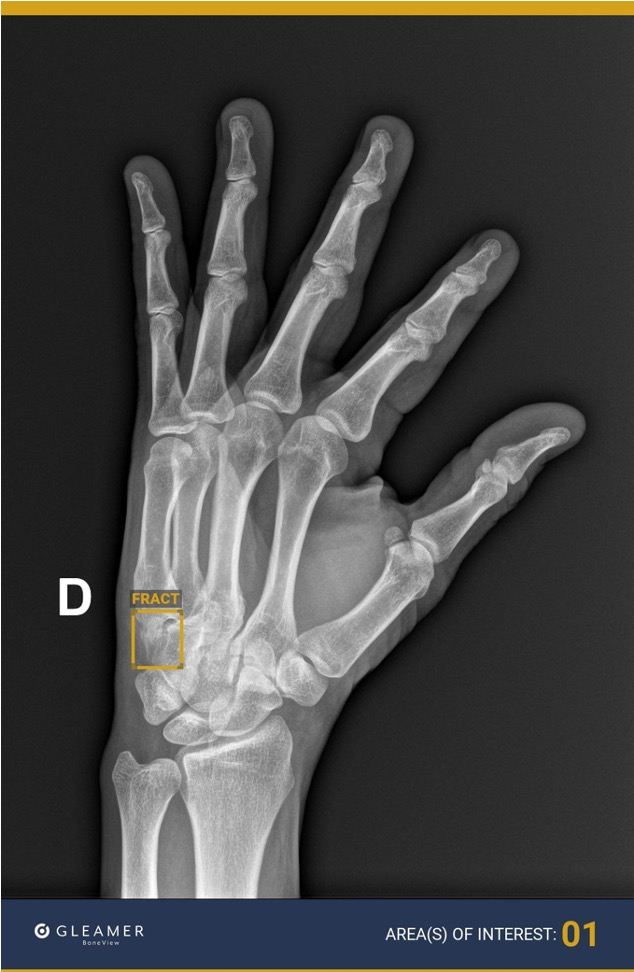
\includegraphics[width=4cm]{data/gleamer.jpeg}
            };
        \end{tikzpicture}
    \end{frame}

	\begin{frame}{AI i hjerneforskning}
        \centering
        \begin{tikzpicture}
            \node[draw=black, fill=white] {
                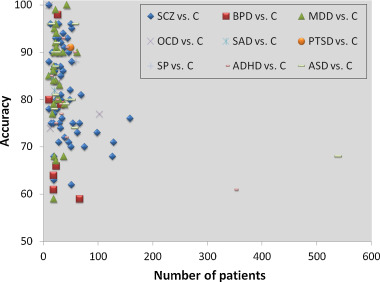
\includegraphics[width=6cm]{data/wolfers.jpg}
            };
        \end{tikzpicture}
    \end{frame}

	\begin{frame}{AI i hjerneforskning}
		\colorlet{rulescolour}{blue!20}
		\colorlet{rulecolour}{cyan!20}

        \centering
        \begin{tikzpicture}
			\node[
				minimum width=2.4cm,
				minimum height=1.6cm,
				draw=black,
				fill=rulescolour,
				label=above:{\textbf{\footnotesize{Regelmotor}}}
			] (rules) at (0, 0) {};

			\node[
				minimum width=1.5cm,
				minimum height=0.3cm,
				draw=black,
				fill=rulecolour
			] (rule1) at ($ (rules) + (0, 0.5) $) {
				\small{Nedstemt}
			};
			\node[
				minimum width=1.5cm,
				minimum height=0.3cm,
				draw=black,
				fill=rulecolour
			] (rule2) at ($ (rules) + (0, 0.0) $) {
				\small{Søvnløshet}
			};
			\node[
				minimum width=1.5cm,
				minimum height=0.3cm,
				draw=black,
				fill=rulecolour
			] (rule3) at ($ (rules) + (0, -0.5) $) {
				\small{Tretthet}
			};
			\draw[] (rules.west) to [in=180, out=0] (rule1.west);
			\draw[] (rules.west) to [in=180, out=0] (rule2.west);
			\draw[] (rules.west) to [in=180, out=0] (rule3.west);

			\draw[] (rule1.east) to [in=180, out=0] (rules.east);
			\draw[] (rule2.east) to [in=180, out=0] (rules.east);
			\draw[] (rule3.east) to [in=180, out=0] (rules.east);

			\def\nodesize{8pt}
			\def\vsep{0.35}
			\def\hsep{0.7}
			\def\arrowstyle{-}

			\node[
				minimum width=2.4cm,
				minimum height=1.6cm,
				draw=black,
				fill=rulescolour,
				label=above:{\textbf{\footnotesize{Regelmotor}}}
			] (rules) at (4, 0) {};

			\node[circle, minimum size=\nodesize, draw=black, fill=rulecolour, inner sep=0pt] (n11) at (rules) {};
			\node[circle, minimum size=\nodesize, draw=black, fill=rulecolour, inner sep=0pt] (n10) at ($ (n11) + (0, \vsep) $) {};
			\node[circle, minimum size=\nodesize, draw=black, fill=rulecolour, inner sep=0pt] (n12) at ($ (n11) + (0, -\vsep) $) {};

			\node[circle, minimum size=\nodesize, draw=black, fill=rulecolour, inner sep=0pt] (n00) at ($ (n11) - (\hsep, -1.5 * \vsep) $) {};
			\node[circle, minimum size=\nodesize, draw=black, fill=rulecolour, inner sep=0pt] (n01) at ($ (n11) - (\hsep, -0.5 * \vsep) $) {};
			\node[circle, minimum size=\nodesize, draw=black, fill=rulecolour, inner sep=0pt] (n02) at ($ (n11) - (\hsep, 0.5 * \vsep) $) {};
			\node[circle, minimum size=\nodesize, draw=black, fill=rulecolour, inner sep=0pt] (n03) at ($ (n11) - (\hsep, 1.5 * \vsep) $) {};

			\node[circle, minimum size=\nodesize, draw=black, fill=rulecolour, inner sep=0pt] (n20) at ($ (n11) + (\hsep, 0.5 * \vsep) $) {};
			\node[circle, minimum size=\nodesize, draw=black, fill=rulecolour, inner sep=0pt] (n21) at ($ (n11) + (\hsep, -0.5 * \vsep) $) {};

			\draw[\arrowstyle] (rules.west) to [in=180, out=0] (n00);
			\draw[\arrowstyle] (rules.west) to [in=180, out=0] (n01);
			\draw[\arrowstyle] (rules.west) to [in=180, out=0] (n02);
			\draw[\arrowstyle] (rules.west) to [in=180, out=0] (n03);

			\draw[\arrowstyle] (n00) to [in=180, out=0] (n10);
			\draw[\arrowstyle] (n00) to [in=180, out=0] (n11);
			\draw[\arrowstyle] (n00) to [in=180, out=0] (n12);
			\draw[\arrowstyle] (n01) to [in=180, out=0] (n10);
			\draw[\arrowstyle] (n01) to [in=180, out=0] (n11);
			\draw[\arrowstyle] (n01) to [in=180, out=0] (n12);
			\draw[\arrowstyle] (n02) to [in=180, out=0] (n10);
			\draw[\arrowstyle] (n02) to [in=180, out=0] (n11);
			\draw[\arrowstyle] (n02) to [in=180, out=0] (n12);
			\draw[\arrowstyle] (n03) to [in=180, out=0] (n10);
			\draw[\arrowstyle] (n03) to [in=180, out=0] (n11);
			\draw[\arrowstyle] (n03) to [in=180, out=0] (n12);

			\draw[\arrowstyle] (n10) to [in=180, out=0] (n20);
			\draw[\arrowstyle] (n10) to [in=180, out=0] (n21);
			\draw[\arrowstyle] (n11) to [in=180, out=0] (n20);
			\draw[\arrowstyle] (n11) to [in=180, out=0] (n21);
			\draw[\arrowstyle] (n12) to [in=180, out=0] (n20);
			\draw[\arrowstyle] (n12) to [in=180, out=0] (n21);

			\draw[\arrowstyle] (n20) to [in=180, out=0] (rules.east);
			\draw[\arrowstyle] (n21) to [in=180, out=0] (rules.east);

        \end{tikzpicture}
    \end{frame}

    \begin{frame}{AI i hjerneforskning: Hjernealder} % Concept
		\centering
        \begin{tikzpicture}
            \node[inner sep=0pt, draw=black] (plot) at (0, 0) {
                
\includegraphics[width=6cm]{data/old-brain.png}
            };
            \node[anchor=north, align=center] at ($ (plot.south) + (0, -0.1) $) {
				\footnotesize{Generert av DALL-E 3 med prompt:}\\
				\footnotesize{"Draw me a cartoon of a brain that looks like an old man"}
            };
        \end{tikzpicture}
    \end{frame}

    \begin{frame}{AI i hjerneforskning: Hjernealder} % Concept Cole
        \centering
        \begin{tikzpicture}
            \node[inner sep=0pt, draw=black] (plot) at (0, 0) {
                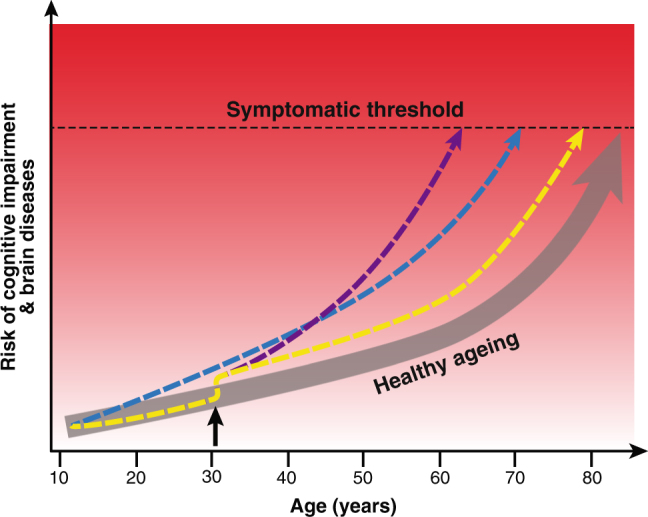
\includegraphics[width=7cm]{data/cole.jpg}
            };
            \node[anchor=north, align=center] at ($ (plot.south) + (0, -0.1) $) {
                \footnotesize{Brain age and other bodily 'ages': implications for neuropsychiatry}\\
                \footnotesize{Cole et al., \textit{Molecular Psychiatry} (2019)}
            };
        \end{tikzpicture}
    \end{frame}

    \begin{frame}{AI i hjerneforskning: Hjernealder} % Datasett
        \centering
        \vfill
		\begin{tikzpicture}
			\pgfplotstableread[col sep=comma]{/Users/esten/phd/papers/2023-explainable-brain-age/data/full_data_distributions.csv}\data
			\begin{axis}[
				width=1\textwidth,
				height=0.85\textwidth,
				xmin=0,
				xmax=100,
				ytick=\empty,
				axis x line=middle,
				axis y line=none,
				xtick={10,20,30,40,50,60,70,80},
				x axis line style={|-stealth},
				clip=false
			]
				\addplot[
					name path=zero,
				] coordinates {(0,0) (100,0)};
				\addplot [
					draw=none,
					line width=0pt,
					name path={female_ds002424},
				] table [
					x=age,
					y expr=1 * \thisrow{female_ds002424}
				]{\data};
				\addplot [
					draw=none,
					line width=0pt,
					name path={female_HBN},
				] table [
					x=age,
					y expr=1 * \thisrow{female_HBN}
				]{\data};
				% \addplot [
				% 	draw=none,
				% 	line width=0pt,
				% 	name path={female_ABCD},
				% ] table [
				% 	x=age,
				% 	y expr=1 * \thisrow{female_ABCD}
				% ]{\data};
				\addplot [
					draw=none,
					line width=0pt,
					name path={female_QTAB},
				] table [
					x=age,
					y expr=1 * \thisrow{female_QTAB}
				]{\data};
				\addplot [
					draw=none,
					line width=0pt,
					name path={female_PING},
				] table [
					x=age,
					y expr=1 * \thisrow{female_PING}
				]{\data};
				\addplot [
					draw=none,
					line width=0pt,
					name path={female_ADHD200},
				] table [
					x=age,
					y expr=1 * \thisrow{female_ADHD200}
				]{\data};
				\addplot [
					draw=none,
					line width=0pt,
					name path={female_PNC},
				] table [
					x=age,
					y expr=1 * \thisrow{female_PNC}
				]{\data};
				\addplot [
					draw=none,
					line width=0pt,
					name path={female_ABIDE II},
				] table [
					x=age,
					y expr=1 * \thisrow{female_ABIDE II}
				]{\data};
				\addplot [
					draw=none,
					line width=0pt,
					name path={female_ds000119},
				] table [
					x=age,
					y expr=1 * \thisrow{female_ds000119}
				]{\data};
				\addplot [
					draw=none,
					line width=0pt,
					name path={female_ABIDE I},
				] table [
					x=age,
					y expr=1 * \thisrow{female_ABIDE I}
				]{\data};
				\addplot [
					draw=none,
					line width=0pt,
					name path={female_BRAINMINT},
				] table [
					x=age,
					y expr=1 * \thisrow{female_BRAINMINT}
				]{\data};
				\addplot [
					draw=none,
					line width=0pt,
					name path={female_SLIM},
				] table [
					x=age,
					y expr=1 * \thisrow{female_SLIM}
				]{\data};
				\addplot [
					draw=none,
					line width=0pt,
					name path={female_QTIM},
				] table [
					x=age,
					y expr=1 * \thisrow{female_QTIM}
				]{\data};
				\addplot [
					draw=none,
					line width=0pt,
					name path={female_Beijing},
				] table [
					x=age,
					y expr=1 * \thisrow{female_Beijing}
				]{\data};
				\addplot [
					draw=none,
					line width=0pt,
					name path={female_AOMIC-PIOP2},
				] table [
					x=age,
					y expr=1 * \thisrow{female_AOMIC-PIOP2}
				]{\data};
				\addplot [
					draw=none,
					line width=0pt,
					name path={female_ds000202},
				] table [
					x=age,
					y expr=1 * \thisrow{female_ds000202}
				]{\data};
				\addplot [
					draw=none,
					line width=0pt,
					name path={female_AOMIC-PIOP1},
				] table [
					x=age,
					y expr=1 * \thisrow{female_AOMIC-PIOP1}
				]{\data};
				\addplot [
					draw=none,
					line width=0pt,
					name path={female_AOMIC-ID1000},
				] table [
					x=age,
					y expr=1 * \thisrow{female_AOMIC-ID1000}
				]{\data};
				\addplot [
					draw=none,
					line width=0pt,
					name path={female_CoRR},
				] table [
					x=age,
					y expr=1 * \thisrow{female_CoRR}
				]{\data};
				\addplot [
					draw=none,
					line width=0pt,
					name path={female_HCP},
				] table [
					x=age,
					y expr=1 * \thisrow{female_HCP}
				]{\data};
				\addplot [
					draw=none,
					line width=0pt,
					name path={female_FCON1000},
				] table [
					x=age,
					y expr=1 * \thisrow{female_FCON1000}
				]{\data};
				\addplot [
					draw=none,
					line width=0pt,
					name path={female_ds000171},
				] table [
					x=age,
					y expr=1 * \thisrow{female_ds000171}
				]{\data};
				\addplot [
					draw=none,
					line width=0pt,
					name path={female_TOP},
				] table [
					x=age,
					y expr=1 * \thisrow{female_TOP}
				]{\data};
				\addplot [
					draw=none,
					line width=0pt,
					name path={female_SCZ-Z},
				] table [
					x=age,
					y expr=1 * \thisrow{female_SCZ-Z}
				]{\data};
				\addplot [
					draw=none,
					line width=0pt,
					name path={female_NIMH},
				] table [
					x=age,
					y expr=1 * \thisrow{female_NIMH}
				]{\data};
				\addplot [
					draw=none,
					line width=0pt,
					name path={female_NKI-RS},
				] table [
					x=age,
					y expr=1 * \thisrow{female_NKI-RS}
				]{\data};
				\addplot [
					draw=none,
					line width=0pt,
					name path={female_MPI-LEMON},
				] table [
					x=age,
					y expr=1 * \thisrow{female_MPI-LEMON}
				]{\data};
				\addplot [
					draw=none,
					line width=0pt,
					name path={female_ds003592},
				] table [
					x=age,
					y expr=1 * \thisrow{female_ds003592}
				]{\data};
				\addplot [
					draw=none,
					line width=0pt,
					name path={female_ds004302},
				] table [
					x=age,
					y expr=1 * \thisrow{female_ds004302}
				]{\data};
				\addplot [
					draw=none,
					line width=0pt,
					name path={female_ds000222},
				] table [
					x=age,
					y expr=1 * \thisrow{female_ds000222}
				]{\data};
				\addplot [
					draw=none,
					line width=0pt,
					name path={female_SALD},
				] table [
					x=age,
					y expr=1 * \thisrow{female_SALD}
				]{\data};
				\addplot [
					draw=none,
					line width=0pt,
					name path={female_IXI},
				] table [
					x=age,
					y expr=1 * \thisrow{female_IXI}
				]{\data};
				\addplot [
					draw=none,
					line width=0pt,
					name path={female_DLBS},
				] table [
					x=age,
					y expr=1 * \thisrow{female_DLBS}
				]{\data};
				\addplot [
					draw=none,
					line width=0pt,
					name path={female_Cam-CAN},
				] table [
					x=age,
					y expr=1 * \thisrow{female_Cam-CAN}
				]{\data};
				\addplot [
					draw=none,
					line width=0pt,
					name path={female_StrokeMRI},
				] table [
					x=age,
					y expr=1 * \thisrow{female_StrokeMRI}
				]{\data};
				\addplot [
					draw=none,
					line width=0pt,
					name path={female_PPMI},
				] table [
					x=age,
					y expr=1 * \thisrow{female_PPMI}
				]{\data};
				\addplot [
					draw=none,
					line width=0pt,
					name path={female_UKBB},
				] table [
					x=age,
					y expr=1 * \thisrow{female_UKBB}
				]{\data};
				\addplot [
					draw=none,
					line width=0pt,
					name path={female_Tao-Wu},
				] table [
					x=age,
					y expr=1 * \thisrow{female_Tao-Wu}
				]{\data};
				\addplot [
					draw=none,
					line width=0pt,
					name path={female_ds000245},
				] table [
					x=age,
					y expr=1 * \thisrow{female_ds000245}
				]{\data};
				\addplot [
					draw=none,
					line width=0pt,
					name path={female_OASIS3},
				] table [
					x=age,
					y expr=1 * \thisrow{female_OASIS3}
				]{\data};
				\addplot [
					draw=none,
					line width=0pt,
					name path={female_Demgen},
				] table [
					x=age,
					y expr=1 * \thisrow{female_Demgen}
				]{\data};
				\addplot [
					draw=none,
					line width=0pt,
					name path={female_NEUROCON},
				] table [
					x=age,
					y expr=1 * \thisrow{female_NEUROCON}
				]{\data};
				\addplot [
					draw=none,
					line width=0pt,
					name path={female_MIRIAD},
				] table [
					x=age,
					y expr=1 * \thisrow{female_MIRIAD}
				]{\data};
				\addplot [
					draw=none,
					line width=0pt,
					name path={female_ds004392},
				] table [
					x=age,
					y expr=1 * \thisrow{female_ds004392}
				]{\data};
				\addplot [
					draw=none,
					line width=0pt,
					name path={female_AIBL},
				] table [
					x=age,
					y expr=1 * \thisrow{female_AIBL}
				]{\data};
				\addplot [
					draw=none,
					line width=0pt,
					name path={female_ANM},
				] table [
					x=age,
					y expr=1 * \thisrow{female_ANM}
				]{\data};
				% \addplot [
				% 	draw=none,
				% 	line width=0pt,
				% 	name path={female_ADNI},
				% ] table [
				% 	x=age,
				% 	y expr=1 * \thisrow{female_ADNI}
				% ]{\data};
				\addplot [
					draw=none,
					line width=0pt,
					name path={male_ds002424},
				] table [
					x=age,
					y expr=-1 * \thisrow{male_ds002424}
				]{\data};
				\addplot [
					draw=none,
					line width=0pt,
					name path={male_HBN},
				] table [
					x=age,
					y expr=-1 * \thisrow{male_HBN}
				]{\data};
				% \addplot [
				% 	draw=none,
				% 	line width=0pt,
				% 	name path={male_ABCD},
				% ] table [
				% 	x=age,
				% 	y expr=-1 * \thisrow{male_ABCD}
				% ]{\data};
				\addplot [
					draw=none,
					line width=0pt,
					name path={male_QTAB},
				] table [
					x=age,
					y expr=-1 * \thisrow{male_QTAB}
				]{\data};
				\addplot [
					draw=none,
					line width=0pt,
					name path={male_PING},
				] table [
					x=age,
					y expr=-1 * \thisrow{male_PING}
				]{\data};
				\addplot [
					draw=none,
					line width=0pt,
					name path={male_ADHD200},
				] table [
					x=age,
					y expr=-1 * \thisrow{male_ADHD200}
				]{\data};
				\addplot [
					draw=none,
					line width=0pt,
					name path={male_PNC},
				] table [
					x=age,
					y expr=-1 * \thisrow{male_PNC}
				]{\data};
				\addplot [
					draw=none,
					line width=0pt,
					name path={male_ABIDE II},
				] table [
					x=age,
					y expr=-1 * \thisrow{male_ABIDE II}
				]{\data};
				\addplot [
					draw=none,
					line width=0pt,
					name path={male_ds000119},
				] table [
					x=age,
					y expr=-1 * \thisrow{male_ds000119}
				]{\data};
				\addplot [
					draw=none,
					line width=0pt,
					name path={male_ABIDE I},
				] table [
					x=age,
					y expr=-1 * \thisrow{male_ABIDE I}
				]{\data};
				\addplot [
					draw=none,
					line width=0pt,
					name path={male_BRAINMINT},
				] table [
					x=age,
					y expr=-1 * \thisrow{male_BRAINMINT}
				]{\data};
				\addplot [
					draw=none,
					line width=0pt,
					name path={male_SLIM},
				] table [
					x=age,
					y expr=-1 * \thisrow{male_SLIM}
				]{\data};
				\addplot [
					draw=none,
					line width=0pt,
					name path={male_QTIM},
				] table [
					x=age,
					y expr=-1 * \thisrow{male_QTIM}
				]{\data};
				\addplot [
					draw=none,
					line width=0pt,
					name path={male_Beijing},
				] table [
					x=age,
					y expr=-1 * \thisrow{male_Beijing}
				]{\data};
				\addplot [
					draw=none,
					line width=0pt,
					name path={male_AOMIC-PIOP2},
				] table [
					x=age,
					y expr=-1 * \thisrow{male_AOMIC-PIOP2}
				]{\data};
				\addplot [
					draw=none,
					line width=0pt,
					name path={male_ds000202},
				] table [
					x=age,
					y expr=-1 * \thisrow{male_ds000202}
				]{\data};
				\addplot [
					draw=none,
					line width=0pt,
					name path={male_AOMIC-PIOP1},
				] table [
					x=age,
					y expr=-1 * \thisrow{male_AOMIC-PIOP1}
				]{\data};
				\addplot [
					draw=none,
					line width=0pt,
					name path={male_AOMIC-ID1000},
				] table [
					x=age,
					y expr=-1 * \thisrow{male_AOMIC-ID1000}
				]{\data};
				\addplot [
					draw=none,
					line width=0pt,
					name path={male_CoRR},
				] table [
					x=age,
					y expr=-1 * \thisrow{male_CoRR}
				]{\data};
				\addplot [
					draw=none,
					line width=0pt,
					name path={male_HCP},
				] table [
					x=age,
					y expr=-1 * \thisrow{male_HCP}
				]{\data};
				\addplot [
					draw=none,
					line width=0pt,
					name path={male_FCON1000},
				] table [
					x=age,
					y expr=-1 * \thisrow{male_FCON1000}
				]{\data};
				\addplot [
					draw=none,
					line width=0pt,
					name path={male_ds000171},
				] table [
					x=age,
					y expr=-1 * \thisrow{male_ds000171}
				]{\data};
				\addplot [
					draw=none,
					line width=0pt,
					name path={male_TOP},
				] table [
					x=age,
					y expr=-1 * \thisrow{male_TOP}
				]{\data};
				\addplot [
					draw=none,
					line width=0pt,
					name path={male_SCZ-Z},
				] table [
					x=age,
					y expr=-1 * \thisrow{male_SCZ-Z}
				]{\data};
				\addplot [
					draw=none,
					line width=0pt,
					name path={male_NIMH},
				] table [
					x=age,
					y expr=-1 * \thisrow{male_NIMH}
				]{\data};
				\addplot [
					draw=none,
					line width=0pt,
					name path={male_NKI-RS},
				] table [
					x=age,
					y expr=-1 * \thisrow{male_NKI-RS}
				]{\data};
				\addplot [
					draw=none,
					line width=0pt,
					name path={male_MPI-LEMON},
				] table [
					x=age,
					y expr=-1 * \thisrow{male_MPI-LEMON}
				]{\data};
				\addplot [
					draw=none,
					line width=0pt,
					name path={male_ds003592},
				] table [
					x=age,
					y expr=-1 * \thisrow{male_ds003592}
				]{\data};
				\addplot [
					draw=none,
					line width=0pt,
					name path={male_ds004302},
				] table [
					x=age,
					y expr=-1 * \thisrow{male_ds004302}
				]{\data};
				\addplot [
					draw=none,
					line width=0pt,
					name path={male_ds000222},
				] table [
					x=age,
					y expr=-1 * \thisrow{male_ds000222}
				]{\data};
				\addplot [
					draw=none,
					line width=0pt,
					name path={male_SALD},
				] table [
					x=age,
					y expr=-1 * \thisrow{male_SALD}
				]{\data};
				\addplot [
					draw=none,
					line width=0pt,
					name path={male_IXI},
				] table [
					x=age,
					y expr=-1 * \thisrow{male_IXI}
				]{\data};
				\addplot [
					draw=none,
					line width=0pt,
					name path={male_DLBS},
				] table [
					x=age,
					y expr=-1 * \thisrow{male_DLBS}
				]{\data};
				\addplot [
					draw=none,
					line width=0pt,
					name path={male_Cam-CAN},
				] table [
					x=age,
					y expr=-1 * \thisrow{male_Cam-CAN}
				]{\data};
				\addplot [
					draw=none,
					line width=0pt,
					name path={male_StrokeMRI},
				] table [
					x=age,
					y expr=-1 * \thisrow{male_StrokeMRI}
				]{\data};
				\addplot [
					draw=none,
					line width=0pt,
					name path={male_PPMI},
				] table [
					x=age,
					y expr=-1 * \thisrow{male_PPMI}
				]{\data};
				\addplot [
					draw=none,
					line width=0pt,
					name path={male_UKBB},
				] table [
					x=age,
					y expr=-1 * \thisrow{male_UKBB}
				]{\data};
				\addplot [
					draw=none,
					line width=0pt,
					name path={male_Tao-Wu},
				] table [
					x=age,
					y expr=-1 * \thisrow{male_Tao-Wu}
				]{\data};
				\addplot [
					draw=none,
					line width=0pt,
					name path={male_ds000245},
				] table [
					x=age,
					y expr=-1 * \thisrow{male_ds000245}
				]{\data};
				\addplot [
					draw=none,
					line width=0pt,
					name path={male_OASIS3},
				] table [
					x=age,
					y expr=-1 * \thisrow{male_OASIS3}
				]{\data};
				\addplot [
					draw=none,
					line width=0pt,
					name path={male_Demgen},
				] table [
					x=age,
					y expr=-1 * \thisrow{male_Demgen}
				]{\data};
				\addplot [
					draw=none,
					line width=0pt,
					name path={male_NEUROCON},
				] table [
					x=age,
					y expr=-1 * \thisrow{male_NEUROCON}
				]{\data};
				\addplot [
					draw=none,
					line width=0pt,
					name path={male_MIRIAD},
				] table [
					x=age,
					y expr=-1 * \thisrow{male_MIRIAD}
				]{\data};
				\addplot [
					draw=none,
					line width=0pt,
					name path={male_ds004392},
				] table [
					x=age,
					y expr=-1 * \thisrow{male_ds004392}
				]{\data};
				\addplot [
					draw=none,
					line width=0pt,
					name path={male_AIBL},
				] table [
					x=age,
					y expr=-1 * \thisrow{male_AIBL}
				]{\data};
				\addplot [
					draw=none,
					line width=0pt,
					name path={male_ANM},
				] table [
					x=age,
					y expr=-1 * \thisrow{male_ANM}
				]{\data};
				% \addplot [
				% 	draw=none,
				% 	line width=0pt,
				% 	name path={male_ADNI},
				% ] table [
				% 	x=age,
				% 	y expr=-1 * \thisrow{male_ADNI}
				% ]{\data};
				\addplot[
					ds002424!50
				] fill between [
					of=zero and female_ds002424
				];
				\addplot[
					ds002424!50
				] fill between [
					of=zero and male_ds002424
				];
				\addplot[
					HBN!50
				] fill between [
					of=female_ds002424 and female_HBN
				];
				\addplot[
					HBN!50
				] fill between [
					of=male_ds002424 and male_HBN
				];
				% \addplot[
				% 	ABCD!50
				% ] fill between [
				% 	of=zero and female_ABCD
				% ];
				% \addplot[
				% 	ABCD!50
				% ] fill between [
				% 	of=zero and male_ABCD
				% ];
				\addplot[
					QTAB!50
				] fill between [
					of=female_HBN and female_QTAB
				];
				\addplot[
					QTAB!50
				] fill between [
					of=male_HBN and male_QTAB
				];
				\addplot[
					PING!50
				] fill between [
					of=female_QTAB and female_PING
				];
				\addplot[
					PING!50
				] fill between [
					of=male_QTAB and male_PING
				];
				\addplot[
					ADHD200!50
				] fill between [
					of=female_PING and female_ADHD200
				];
				\addplot[
					ADHD200!50
				] fill between [
					of=male_PING and male_ADHD200
				];
				\addplot[
					PNC!50
				] fill between [
					of=female_ADHD200 and female_PNC
				];
				\addplot[
					PNC!50
				] fill between [
					of=male_ADHD200 and male_PNC
				];
				\addplot[
					ABIDE II!50
				] fill between [
					of=female_PNC and female_ABIDE II
				];
				\addplot[
					ABIDE II!50
				] fill between [
					of=male_PNC and male_ABIDE II
				];
				\addplot[
					ds000119!50
				] fill between [
					of=female_ABIDE II and female_ds000119
				];
				\addplot[
					ds000119!50
				] fill between [
					of=male_ABIDE II and male_ds000119
				];
				\addplot[
					ABIDE I!50
				] fill between [
					of=female_ds000119 and female_ABIDE I
				];
				\addplot[
					ABIDE I!50
				] fill between [
					of=male_ds000119 and male_ABIDE I
				];
				\addplot[
					BRAINMINT!50
				] fill between [
					of=female_ABIDE I and female_BRAINMINT
				];
				\addplot[
					BRAINMINT!50
				] fill between [
					of=male_ABIDE I and male_BRAINMINT
				];
				\addplot[
					SLIM!50
				] fill between [
					of=female_BRAINMINT and female_SLIM
				];
				\addplot[
					SLIM!50
				] fill between [
					of=male_BRAINMINT and male_SLIM
				];
				\addplot[
					QTIM!50
				] fill between [
					of=female_SLIM and female_QTIM
				];
				\addplot[
					QTIM!50
				] fill between [
					of=male_SLIM and male_QTIM
				];
				\addplot[
					Beijing!50
				] fill between [
					of=female_QTIM and female_Beijing
				];
				\addplot[
					Beijing!50
				] fill between [
					of=male_QTIM and male_Beijing
				];
				\addplot[
					AOMIC-PIOP2!50
				] fill between [
					of=female_Beijing and female_AOMIC-PIOP2
				];
				\addplot[
					AOMIC-PIOP2!50
				] fill between [
					of=male_Beijing and male_AOMIC-PIOP2
				];
				\addplot[
					ds000202!50
				] fill between [
					of=female_AOMIC-PIOP2 and female_ds000202
				];
				\addplot[
					ds000202!50
				] fill between [
					of=male_AOMIC-PIOP2 and male_ds000202
				];
				\addplot[
					AOMIC-PIOP1!50
				] fill between [
					of=female_ds000202 and female_AOMIC-PIOP1
				];
				\addplot[
					AOMIC-PIOP1!50
				] fill between [
					of=male_ds000202 and male_AOMIC-PIOP1
				];
				\addplot[
					AOMIC-ID1000!50
				] fill between [
					of=female_AOMIC-PIOP1 and female_AOMIC-ID1000
				];
				\addplot[
					AOMIC-ID1000!50
				] fill between [
					of=male_AOMIC-PIOP1 and male_AOMIC-ID1000
				];
				\addplot[
					CoRR!50
				] fill between [
					of=female_AOMIC-ID1000 and female_CoRR
				];
				\addplot[
					CoRR!50
				] fill between [
					of=male_AOMIC-ID1000 and male_CoRR
				];
				\addplot[
					HCP!50
				] fill between [
					of=female_CoRR and female_HCP
				];
				\addplot[
					HCP!50
				] fill between [
					of=male_CoRR and male_HCP
				];
				\addplot[
					FCON1000!50
				] fill between [
					of=female_HCP and female_FCON1000
				];
				\addplot[
					FCON1000!50
				] fill between [
					of=male_HCP and male_FCON1000
				];
				\addplot[
					ds000171!50
				] fill between [
					of=female_FCON1000 and female_ds000171
				];
				\addplot[
					ds000171!50
				] fill between [
					of=male_FCON1000 and male_ds000171
				];
				\addplot[
					TOP!50
				] fill between [
					of=female_ds000171 and female_TOP
				];
				\addplot[
					TOP!50
				] fill between [
					of=male_ds000171 and male_TOP
				];
				\addplot[
					SCZ-Z!50
				] fill between [
					of=female_TOP and female_SCZ-Z
				];
				\addplot[
					SCZ-Z!50
				] fill between [
					of=male_TOP and male_SCZ-Z
				];
				\addplot[
					NIMH!50
				] fill between [
					of=female_SCZ-Z and female_NIMH
				];
				\addplot[
					NIMH!50
				] fill between [
					of=male_SCZ-Z and male_NIMH
				];
				\addplot[
					NKI-RS!50
				] fill between [
					of=female_NIMH and female_NKI-RS
				];
				\addplot[
					NKI-RS!50
				] fill between [
					of=male_NIMH and male_NKI-RS
				];
				\addplot[
					MPI-LEMON!50
				] fill between [
					of=female_NKI-RS and female_MPI-LEMON
				];
				\addplot[
					MPI-LEMON!50
				] fill between [
					of=male_NKI-RS and male_MPI-LEMON
				];
				\addplot[
					ds003592!50
				] fill between [
					of=female_MPI-LEMON and female_ds003592
				];
				\addplot[
					ds003592!50
				] fill between [
					of=male_MPI-LEMON and male_ds003592
				];
				\addplot[
					ds004302!50
				] fill between [
					of=female_ds003592 and female_ds004302
				];
				\addplot[
					ds004302!50
				] fill between [
					of=male_ds003592 and male_ds004302
				];
				\addplot[
					ds000222!50
				] fill between [
					of=female_ds004302 and female_ds000222
				];
				\addplot[
					ds000222!50
				] fill between [
					of=male_ds004302 and male_ds000222
				];
				\addplot[
					SALD!50
				] fill between [
					of=female_ds000222 and female_SALD
				];
				\addplot[
					SALD!50
				] fill between [
					of=male_ds000222 and male_SALD
				];
				\addplot[
					IXI!50
				] fill between [
					of=female_SALD and female_IXI
				];
				\addplot[
					IXI!50
				] fill between [
					of=male_SALD and male_IXI
				];
				\addplot[
					DLBS!50
				] fill between [
					of=female_IXI and female_DLBS
				];
				\addplot[
					DLBS!50
				] fill between [
					of=male_IXI and male_DLBS
				];
				\addplot[
					Cam-CAN!50
				] fill between [
					of=female_DLBS and female_Cam-CAN
				];
				\addplot[
					Cam-CAN!50
				] fill between [
					of=male_DLBS and male_Cam-CAN
				];
				\addplot[
					StrokeMRI!50
				] fill between [
					of=female_Cam-CAN and female_StrokeMRI
				];
				\addplot[
					StrokeMRI!50
				] fill between [
					of=male_Cam-CAN and male_StrokeMRI
				];
				\addplot[
					PPMI!50
				] fill between [
					of=female_StrokeMRI and female_PPMI
				];
				\addplot[
					PPMI!50
				] fill between [
					of=male_StrokeMRI and male_PPMI
				];
				\addplot[
					UKBB!50
				] fill between [
					of=female_PPMI and female_UKBB
				];
				\addplot[
					UKBB!50
				] fill between [
					of=male_PPMI and male_UKBB
				];
				\addplot[
					Tao-Wu!50
				] fill between [
					of=female_UKBB and female_Tao-Wu
				];
				\addplot[
					Tao-Wu!50
				] fill between [
					of=male_UKBB and male_Tao-Wu
				];
				\addplot[
					ds000245!50
				] fill between [
					of=female_Tao-Wu and female_ds000245
				];
				\addplot[
					ds000245!50
				] fill between [
					of=male_Tao-Wu and male_ds000245
				];
				\addplot[
					OASIS3!50
				] fill between [
					of=female_ds000245 and female_OASIS3
				];
				\addplot[
					OASIS3!50
				] fill between [
					of=male_ds000245 and male_OASIS3
				];
				\addplot[
					Demgen!50
				] fill between [
					of=female_OASIS3 and female_Demgen
				];
				\addplot[
					Demgen!50
				] fill between [
					of=male_OASIS3 and male_Demgen
				];
				\addplot[
					NEUROCON!50
				] fill between [
					of=female_Demgen and female_NEUROCON
				];
				\addplot[
					NEUROCON!50
				] fill between [
					of=male_Demgen and male_NEUROCON
				];
				\addplot[
					MIRIAD!50
				] fill between [
					of=female_NEUROCON and female_MIRIAD
				];
				\addplot[
					MIRIAD!50
				] fill between [
					of=male_NEUROCON and male_MIRIAD
				];
				\addplot[
					ds004392!50
				] fill between [
					of=female_MIRIAD and female_ds004392
				];
				\addplot[
					ds004392!50
				] fill between [
					of=male_MIRIAD and male_ds004392
				];
				\addplot[
					AIBL!50
				] fill between [
					of=female_ds004392 and female_AIBL
				];
				\addplot[
					AIBL!50
				] fill between [
					of=male_ds004392 and male_AIBL
				];
				\addplot[
					ANM!50
				] fill between [
					of=female_AIBL and female_ANM
				];
				\addplot[
					ANM!50
				] fill between [
					of=male_AIBL and male_ANM
				];
				% \addplot[
				% 	ADNI!50
				% ] fill between [
				% 	of=female_ANM and female_ADNI
				% ];
				% \addplot[
				% 	ADNI!50
				% ] fill between [
				% 	of=male_ANM and male_ADNI
				% ];
				\node[
					anchor=south east
				] at (axis cs: 99, 0.0){KVINNER};
				\node[
					anchor=north east
				] at (axis cs: 99, -0.0){MENN};
                \node[] at (axis cs: 50, -0.7) {MR-scans fra 53,542 deltakere};
			\end{axis}
		\end{tikzpicture}
        \vfill
	\end{frame}

    \begin{frame}{AI i hjerneforskning: Hjernealder} % Modelling
        \newsavebox{\normbox}
        \sbox{\normbox}{%
            \begin{tikzpicture}
                \begin{axis}[
                    width=3cm,
                    height=3cm,
                    ymajorticks=false,
                    xmajorticks=false,
                    xmin=0,
                    ymin=3,
                    xmax=1,
                    ymax=6
                ]
                    \addplot[domain=0:1, samples=100]  {
                        5 + ln(x+0.15)
                    };
                    \addplot[domain=0:1, samples=100, dashed]  {
                        6.5 + ln(0.4*x+0.05)
                    };
                    \addplot[domain=0:1, samples=100, dashed]  {
                        4.25 + ln(x+0.225)
                    };
                \end{axis}
            \end{tikzpicture}
        }
        \centering
        \vfill
		\begin{tikzpicture}[scale=0.9]
            \newcommand{\mrivsep}{0.52}
			\newcommand{\mrihsep}{0.44}
			\def\plotwidth{11.68}

			\newcommand{\nodesize}{11pt}
			\newcommand{\hsep}{28pt}
			\newcommand{\vsep}{14pt}

			\newcommand{\arrowwidth}{0.05cm}
			\newcommand{\innerarrow}{{Latex[length=0.1cm, width=0.15cm]}}
			\newcommand{\outerarrow}{{Latex[length=0.2cm, width=0.3cm]}}

			\definecolor{cb-green}{HTML}{4dac93}
			\definecolor{cb-blue}{HTML}{3594d6}
			\definecolor{outercolor}{RGB}{128, 128, 128}
			\colorlet{train-fill}{cb-blue}

			\newcommand{\patientlocation}[1]{($ (1, -1.6) + ####1 $)}
			\newcommand{\controllocation}[1]{($ (1, -2.8) + ####1 $)}
			\newcommand{\modellocation}[1]{($ (0.5 * \plotwidth, -2.2) + ####1 $)}

            \node[label={[label distance=-0.1cm]below:\footnotesize{75}}] (p0) at (2, -1.1) {
                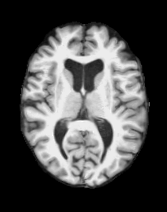
\includegraphics[width=0.6cm]{data/samples/control_0.png}
            };

            \node[label={[label distance=-0.1cm]below:\footnotesize{32}}] (p0) at (1.1, -0.7) {
                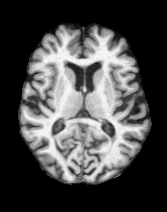
\includegraphics[width=0.6cm]{data/samples/control_1.png}
            };

            \node[label={[label distance=-0.1cm]below:\footnotesize{49}}] (p0) at (1.25, -1.9) {
                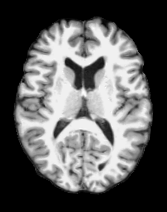
\includegraphics[width=0.6cm]{data/samples/control_2.png}
            };

            \node[label={[label distance=-0.1cm]below:\footnotesize{51}}] (p0) at (0.4, -1.4) {
                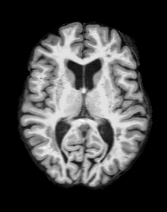
\includegraphics[width=0.6cm]{data/samples/control_3.png}
            };

            \node[label={[label distance=-0.1cm]below:\footnotesize{83}}] (p0) at (2.2, -3) {
                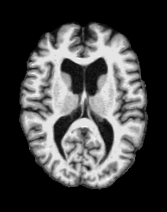
\includegraphics[width=0.6cm]{data/samples/control_4.png}
            };

            \node[label={[label distance=-0.1cm]below:\footnotesize{27}}] (p0) at (1.4, -3.2) {
                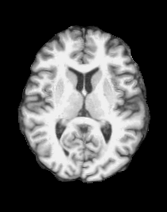
\includegraphics[width=0.6cm]{data/samples/control_5.png}
            };

            \node[label={[label distance=-0.1cm]below:\footnotesize{92}}] (p0) at (0.4, -2.7) {
                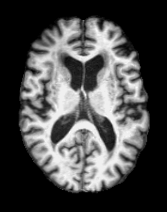
\includegraphics[width=0.6cm]{data/samples/dementia_0.png}
            };

			\node[circle, inner sep=0pt, fill=none, outer sep=0pt, line width=0pt, draw=none] (n00) at \modellocation{(-3 * \hsep, 0)} {};

			\node[circle, minimum size=\nodesize, inner sep=0pt, fill=train-fill!35, outer sep=0pt, line width=0pt, draw=train-fill!35] (n10) at \modellocation{(-2 * \hsep, 2 * \vsep)} {};
			\node[circle, minimum size=\nodesize, inner sep=0pt, fill=train-fill, outer sep=0pt, line width=0pt, draw=train-fill] (n11) at \modellocation{(-2 * \hsep, 1 * \vsep)} {};
			\node[circle, minimum size=\nodesize, inner sep=0pt, fill=train-fill!15, outer sep=0pt, line width=0pt, draw=train-fill!15] (n12) at \modellocation{(-2 * \hsep, 0)} {};
			\node[circle, minimum size=\nodesize, inner sep=0pt, fill=train-fill!85, outer sep=0pt, line width=0pt, draw=train-fill!85] (n13) at \modellocation{(-2 * \hsep, -1 * \vsep)} {};
			\node[circle, minimum size=\nodesize, inner sep=0pt, fill=train-fill!90, outer sep=0pt, line width=0pt, draw=train-fill!90] (n14) at \modellocation{(-2 * \hsep, -2 * \vsep)} {};

			\node[circle, minimum size=\nodesize, inner sep=0pt, fill=train-fill!55, outer sep=0pt, line width=0pt, draw=train-fill!55] (n20) at \modellocation{(-1 * \hsep, 1.5 * \vsep)} {};
			\node[circle, minimum size=\nodesize, inner sep=0pt, fill=train-fill!20, outer sep=0pt, line width=0pt, draw=train-fill!20] (n21) at \modellocation{(-1 * \hsep, 0.5 * \vsep)} {};
			\node[circle, minimum size=\nodesize, inner sep=0pt, fill=train-fill!90, outer sep=0pt, line width=0pt, draw=train-fill!50] (n22) at \modellocation{(-1 * \hsep, -0.5 * \vsep)} {};
			\node[circle, minimum size=\nodesize, inner sep=0pt, fill=train-fill!35, outer sep=0pt, line width=0pt, draw=train-fill!35] (n23) at \modellocation{(-1 * \hsep, -1.5 * \vsep)} {};

			\node[circle, minimum size=\nodesize, inner sep=0pt, fill=train-fill!95, outer sep=0pt, line width=0pt, draw=train-fill!65] (n30) at \modellocation{(0 * \hsep, 1.5 * \vsep)} {};
			\node[circle, minimum size=\nodesize, inner sep=0pt, fill=train-fill!20, outer sep=0pt, line width=0pt, draw=train-fill!20] (n31) at \modellocation{(0 * \hsep, 0.5 * \vsep)} {};
			\node[circle, minimum size=\nodesize, inner sep=0pt, fill=train-fill!90, outer sep=0pt, line width=0pt, draw=train-fill!90] (n32) at \modellocation{(0 * \hsep, -0.5 * \vsep)} {};
			\node[circle, minimum size=\nodesize, inner sep=0pt, fill=train-fill!80, outer sep=0pt, line width=0pt, draw=train-fill!80] (n33) at \modellocation{(0 * \hsep, -1.5 * \vsep)} {};

			\node[circle, minimum size=\nodesize, inner sep=0pt, fill=train-fill!50, outer sep=0pt, line width=0pt, draw=train-fill!50] (n40) at \modellocation{(1 * \hsep, 1*\vsep)} {};
			\node[circle, minimum size=\nodesize, inner sep=0pt, fill=train-fill!90, outer sep=0pt, line width=0pt, draw=train-fill!70] (n41) at \modellocation{(1 * \hsep, 0*\vsep)} {};
			\node[circle, minimum size=\nodesize, inner sep=0pt, fill=train-fill!70, outer sep=0pt, line width=0pt, draw=train-fill!30] (n42) at \modellocation{(1 * \hsep, -1*\vsep)} {};

			\node[circle, minimum size=\nodesize, inner sep=0pt, fill=train-fill, outer sep=0pt, line width=0pt, draw=train-fill] (n50) at \modellocation{(2 * \hsep, 1*\vsep)} {};
			\node[circle, minimum size=\nodesize, inner sep=0pt, fill=train-fill!70, outer sep=0pt, line width=0pt, draw=train-fill!70] (n51) at \modellocation{(2 * \hsep, 0*\vsep)} {};
			\node[circle, minimum size=\nodesize, inner sep=0pt, fill=train-fill!30, outer sep=0pt, line width=0pt, draw=train-fill!30] (n52) at \modellocation{(2 * \hsep, -1*\vsep)} {};

			\node[circle, minimum size=\nodesize, inner sep=0pt, fill=train-fill!80, outer sep=0pt, line width=0pt, draw=train-fill!65] (n60) at \modellocation{(3 * \hsep, 0)} {};

			\node[align=left, font=\linespread{0.8}\selectfont] (loss) at (0.5+2.1*4.85, -2.2) {\usebox{\normbox}};

			\draw[
				color=train-fill!35,
				-\innerarrow,
				line width=\arrowwidth
			] (n00) to [out=20,in=200] (n10) {};
			\draw[
				color=train-fill,
				-\innerarrow,
				line width=\arrowwidth
			] (n00) to [out=10,in=190] (n11) {};
			\draw[
				color=train-fill!15,
				-\innerarrow,
				line width=\arrowwidth
			] (n00) to [out=0,in=180] (n12) {};
			\draw[
				color=train-fill!85,
				-\innerarrow,
				line width=\arrowwidth
			] (n00) to [out=-10,in=170] (n13) {};
			\draw[
				color=train-fill!90,
				-\innerarrow,
				line width=\arrowwidth
			] (n00) to [out=-20,in=160] (n14) {};

			\draw[
				color=train-fill!35,
				-\innerarrow,
				line width=\arrowwidth
			] (n10) to [out=-5,in=175] (n20) {};
			\draw[
				color=train-fill!10,
				-\innerarrow,
				line width=\arrowwidth
			] (n10) to [out=-15,in=165] (n21) {};
			\draw[
				color=train-fill!70,
				-\innerarrow,
				line width=\arrowwidth
			] (n10) to [out=-25,in=155] (n22) {};
			\draw[
				color=train-fill!50,
				-\innerarrow,
				line width=\arrowwidth
			] (n10) to [out=-35,in=145] (n23) {};

			\draw[
				color=train-fill!30,
				-\innerarrow,
				line width=\arrowwidth
			] (n11) to [out=5,in=185] (n20) {};
			\draw[
				color=train-fill!25,
				-\innerarrow,
				line width=\arrowwidth
			] (n11) to [out=-5,in=175] (n21) {};
			\draw[
				color=train-fill!95,
				-\innerarrow,
				line width=\arrowwidth
			] (n11) to [out=-15,in=165] (n22) {};
			\draw[
				color=train-fill!35,
				-\innerarrow,
				line width=\arrowwidth
			] (n11) to [out=-25,in=155] (n23) {};

			\draw[
				color=train-fill!70,
				-\innerarrow,
				line width=\arrowwidth
			] (n12) to [out=15,in=195] (n20) {};
			\draw[
				color=train-fill!20,
				-\innerarrow,
				line width=\arrowwidth
			] (n12) to [out=5,in=185] (n21) {};
			\draw[
				color=train-fill!80,
				-\innerarrow,
				line width=\arrowwidth
			] (n12) to [out=-5,in=175] (n22) {};
			\draw[
				color=train-fill,
				-\innerarrow,
				line width=\arrowwidth
			] (n12) to [out=-15,in=165] (n23) {};

			\draw[
				color=train-fill!40,
				-\innerarrow,
				line width=\arrowwidth
			] (n13) to [out=25,in=205] (n20) {};
			\draw[
				color=train-fill!35,
				-\innerarrow,
				line width=\arrowwidth
			] (n13) to [out=15,in=195] (n21) {};
			\draw[
				color=train-fill!20,
				-\innerarrow,
				line width=\arrowwidth
			] (n13) to [out=5,in=185] (n22) {};
			\draw[
				color=white,
				-\innerarrow,
				line width=\arrowwidth
			] (n13) to [out=-5,in=175] (n23) {};

			\draw[
				color=train-fill!40,
				-\innerarrow,
				line width=\arrowwidth
			] (n14) to [out=35,in=215] (n20) {};
			\draw[
				color=train-fill!85,
				-\innerarrow,
				line width=\arrowwidth
			] (n14) to [out=25,in=205] (n21) {};
			\draw[
				color=train-fill!35,
				-\innerarrow,
				line width=\arrowwidth
			] (n14) to [out=15,in=195] (n22) {};
			\draw[
				color=train-fill,
				-\innerarrow,
				line width=\arrowwidth
			] (n14) to [out=5,in=185] (n23) {};

			\draw[
				color=train-fill!85,
				-\innerarrow,
				line width=\arrowwidth
			] (n20) to [out=0,in=180] (n30) {};
			\draw[
				color=train-fill!50,
				-\innerarrow,
				line width=\arrowwidth
			] (n20) to [out=-10,in=170] (n31) {};
			\draw[
				color=train-fill!75,
				-\innerarrow,
				line width=\arrowwidth
			] (n20) to [out=-20,in=160] (n32) {};
			\draw[
				color=white,
				-\innerarrow,
				line width=\arrowwidth
			] (n20) to [out=-30,in=150] (n33) {};

			\draw[
				color=train-fill,
				-\innerarrow,
				line width=\arrowwidth
			] (n21) to [out=10,in=190] (n30) {};
			\draw[
				color=train-fill!30,
				-\innerarrow,
				line width=\arrowwidth
			] (n21) to [out=0,in=180] (n31) {};
			\draw[
				color=train-fill!25,
				-\innerarrow,
				line width=\arrowwidth
			] (n21) to [out=-10,in=170] (n32) {};
			\draw[
				color=white,
				-\innerarrow,
				line width=\arrowwidth
			] (n21) to [out=-20,in=160] (n33) {};

			\draw[
				color=train-fill!35,
				-\innerarrow,
				line width=\arrowwidth
			] (n22) to [out=20,in=200] (n30) {};
			\draw[
				color=train-fill!95,
				-\innerarrow,
				line width=\arrowwidth
			] (n22) to [out=10,in=190] (n31) {};
			\draw[
				color=train-fill!80,
				-\innerarrow,
				line width=\arrowwidth
			] (n22) to [out=0,in=180] (n32) {};
			\draw[
				color=white,
				-\innerarrow,
				line width=\arrowwidth
			] (n22) to [out=-10,in=170] (n33) {};

			\draw[
				color=train-fill!45,
				-\innerarrow,
				line width=\arrowwidth
			] (n23) to [out=30,in=210] (n30) {};
			\draw[
				color=train-fill!70,
				-\innerarrow,
				line width=\arrowwidth
			] (n23) to [out=20,in=200] (n31) {};
			\draw[
				color=train-fill!10,
				-\innerarrow,
				line width=\arrowwidth
			] (n23) to [out=10,in=190] (n32) {};
			\draw[
				color=train-fill!20,
				-\innerarrow,
				line width=\arrowwidth
			] (n23) to [out=0,in=180] (n33) {};

			\draw[
				color=train-fill!50,
				-\innerarrow,
				line width=\arrowwidth
			] (n30) to [out=-5,in=175] (n40) {};
			\draw[
				color=train-fill!30,
				-\innerarrow,
				line width=\arrowwidth
			] (n30) to [out=-15,in=165] (n41) {};
			\draw[
				color=train-fill,
				-\innerarrow,
				line width=\arrowwidth
			] (n30) to [out=-25,in=155] (n42) {};

			\draw[
				color=train-fill!45,
				-\innerarrow,
				line width=\arrowwidth
			] (n31) to [out=5,in=185] (n40) {};
			\draw[
				color=train-fill!90,
				-\innerarrow,
				line width=\arrowwidth
			] (n31) to [out=-5,in=175] (n41) {};
			\draw[
				color=train-fill!45,
				-\innerarrow,
				line width=\arrowwidth
			] (n31) to [out=-15,in=165] (n42) {};

			\draw[
				color=train-fill!15,
				-\innerarrow,
				line width=\arrowwidth
			] (n32) to [out=15,in=195] (n40) {};
			\draw[
				color=train-fill!70,
				-\innerarrow,
				line width=\arrowwidth
			] (n32) to [out=5,in=185] (n41) {};
			\draw[
				color=train-fill!50,
				-\innerarrow,
				line width=\arrowwidth
			] (n32) to [out=-5,in=175] (n42) {};

			\draw[
				color=train-fill!40,
				-\innerarrow,
				line width=\arrowwidth
			] (n33) to [out=25,in=205] (n40) {};
			\draw[
				color=train-fill!20,
				-\innerarrow,
				line width=\arrowwidth
			] (n33) to [out=15,in=195] (n41) {};
			\draw[
				color=train-fill!90,
				-\innerarrow,
				line width=\arrowwidth
			] (n33) to [out=5,in=185] (n42) {};

			\draw[
				color=train-fill!25,
				-\innerarrow,
				line width=\arrowwidth
			] (n40) to [out=0,in=180] (n50) {};
			\draw[
				color=train-fill!15,
				-\innerarrow,
				line width=\arrowwidth
			] (n40) to [out=-10,in=170] (n51) {};
			\draw[
				color=train-fill,
				-\innerarrow,
				line width=\arrowwidth
			] (n40) to [out=-20,in=160] (n52) {};

			\draw[
				color=train-fill!35,
				-\innerarrow,
				line width=\arrowwidth
			] (n41) to [out=10,in=190] (n50) {};
			\draw[
				color=train-fill!10,
				-\innerarrow,
				line width=\arrowwidth
			] (n41) to [out=0,in=180] (n51) {};
			\draw[
				color=train-fill!90,
				-\innerarrow,
				line width=\arrowwidth
			] (n41) to [out=-10,in=170] (n52) {};

			\draw[
				color=train-fill!50,
				-\innerarrow,
				line width=\arrowwidth
			] (n42) to [out=20,in=200] (n50) {};
			\draw[
				color=train-fill!40,
				-\innerarrow,
				line width=\arrowwidth
			] (n42) to [out=10,in=190] (n51) {};
			\draw[
				color=train-fill!20,
				-\innerarrow,
				line width=\arrowwidth
			] (n42) to [out=0,in=180] (n52) {};

			\draw[
				color=train-fill!80,
				-\innerarrow,
				line width=\arrowwidth,
			] (n50) to [out=-10,in=170] (n60) {};
			\draw[
				color=train-fill!90,
				-\innerarrow,
				line width=\arrowwidth,
			] (n51) to [out=0,in=180] (n60) {};
			\draw[
				color=train-fill!30,
				-\innerarrow,
				line width=\arrowwidth,
			] (n52) to [out=10,in=190] (n60) {};

			\draw[black] (n00.center) --
							($ (n00) + (0, 2*\vsep+0.5*\nodesize+2pt) $) --
							($ (n00) + (6*\hsep+0.5*\nodesize+2pt, 2*\vsep+0.5*\nodesize+2pt) $) --
							($ (n00) + (6*\hsep+0.5*\nodesize+2pt, -2*\vsep-0.5*\nodesize-2pt) $) --
							($ (n00) + (0, -2*\vsep-0.5*\nodesize-2pt) $) --
							(n00.center);

			\node[] at ($ (n30) + (0, \vsep+0.5*\nodesize) $) {Konvolusjonelt nevralt nett};

			\draw[
				color=outercolor,
				-\outerarrow,
				line width=0.1cm
			] ($ (n00.west) - (1, 0) $) to [out=0,in=180] (n00) {};

            \draw[
				color=outercolor,
				-\outerarrow,
				line width=0.1cm
			] ($ (n00.west) - (0.9, 0.35) $) to [out=90,in=180] (n00) {};
            \draw[
				color=outercolor,
				-\outerarrow,
				line width=0.1cm
			] ($ (n00.west) - (0.9, -0.35) $) to [out=270,in=180] (n00) {};
			\draw[
				color=outercolor,
				-\outerarrow,
				line width=0.1cm
			] (n60) to [out=0,in=180] (loss) {};
		\end{tikzpicture}
        \vfill
	\end{frame}

    \begin{frame}{AI i hjerneforskning: Hjernealder} % Predictions
		\def\N{1}
		\centering
		\vfill
		\begin{tikzpicture}
			\begin{groupplot}[
				group style={
					group size=2 by 1,
					horizontal sep=1.2cm,
					vertical sep=0.8cm
				},
				width=0.7\linewidth,
				height=0.7\linewidth
			]

				\nextgroupplot[
					xmin=0,
					xmax=100,
					ymin=0,
					ymax=100,
					xtick pos=bottom,
					ytick pos=left,
					ticklabel style = {font=\footnotesize}
				]
					\addplot [red] coordinates {(0,0) (100,100)};
					\addplot [
						only marks,
						mark size=1.5pt,
						color=black,
						opacity=0.35
					] table [
						x=regression,
						y=age,
						each nth point={\N},
						col sep=comma
					] {data/external_predictions.csv};
					\node [anchor=south east,inner sep=0pt,outer sep=0pt] (outofsample) at (rel axis cs:0.92,0.08) {\textcolor{red}{MAE=3.90}};
			\end{groupplot}
	  \end{tikzpicture}
	  \vfill
	\end{frame}

	\begin{frame}{AI i hjerneforskning: Hjernealder} % Associations
		\definecolor{pwas}{HTML}{70F3FF}
		\definecolor{neg}{HTML}{AAFF99}
		\definecolor{pos}{HTML}{FF8585}
		\definecolor{bars}{HTML}{A899FF}

        \centering
        \vfill

  		\begin{columns}[T]
    		\column{0.6\textwidth}
				\begin{tikzpicture}
					\begin{axis}[
							width=1.15\textwidth,
							height=\textwidth,
							ylabel=$-\mathrm{log}_{10}(p)$,
							y label style={at={(-0.06, 0.5)}},
							ymin=0,
							ymax=11.5,
							xmin=-1,
							xmax=395,
							ytick={2,4,6,8,10},
							yticklabels={-2,-4,-6,-8,-10},
							axis x line*=bottom,
							axis y line=left,
							xtick={32.5,102.5,149.5,177.5,208.5,
								233,254.5,275.5,301.5,334.5,
								358,372,388},
							xticklabels={1,2,3,4,5,6,7,8,9,10,
										11,12,13},
							tick label style={font=\scriptsize},
							clip=false,
							xlabel={Categories}
						]
						\addplot[draw=black, only marks, mark size=1.5pt, fill=pwas] table [x=x,y=y,col sep=comma] {data/pwas.csv};
						\addplot[draw=black,dashed] coordinates {(-1, 3.896) (395, 3.896)};
						\addplot[draw=black,dotted] coordinates {(65,0) (65,11.5)};
						\addplot[draw=black,dotted] coordinates {(140,0) (140,11.5)};
						\addplot[draw=black,dotted] coordinates {(159,0) (159,11.5)};
						\addplot[draw=black,dotted] coordinates {(196,0) (196,11.5)};
						\addplot[draw=black,dotted] coordinates {(221,0) (221,11.5)};
						\addplot[draw=black,dotted] coordinates {(245,0) (245,11.5)};
						\addplot[draw=black,dotted] coordinates {(264,0) (264,11.5)};
						\addplot[draw=black,dotted] coordinates {(287,0) (287,11.5)};
						\addplot[draw=black,dotted] coordinates {(316,0) (316,11.5)};
						\addplot[draw=black,dotted] coordinates {(353,0) (353,11.5)};
						\addplot[draw=black,dotted] coordinates {(363,0) (363,11.5)};
						\addplot[draw=black,dotted] coordinates {(381,0) (381,11.5)};
						\addplot[draw=black,dotted] coordinates {(395,0) (395,11.5)};
						\node[anchor=south] at (axis cs:12,6.09) {\tiny{HbA1c}};
						\node[anchor=south] at (axis cs:18,10.49) {\tiny{Glucose}};
						\node[anchor=north] at (axis cs:26,10.23) {\tiny{IGF-1}};
						\node[anchor=south] at (axis cs:49,4.47) {\tiny{Corpuscular volume}};
						\node[anchor=south, align=center] at (axis cs:65,6.72) {\tiny{Vascular/heart}\\[-1.5ex] \tiny{problem}};
						\node[anchor=south, align=center] at (axis cs:89,9.93) {\tiny{Blood pressure}\\[-1.5ex] \tiny{medication}};
						\node[anchor=south] at (axis cs:128,6.64) {\tiny{Diabetes}};
						\node[anchor=south] at (axis cs:254,6.94) {\tiny{Weekly beer/cider intake}};
						\node[anchor=south, align=center] at (axis cs:303,4.61) {\tiny{Total cigarette}\\[-1.5ex] \tiny{packs}};
						\node[anchor=south, align=center] at (axis cs:376,5.33) {\tiny{Non-UK country}\\[-1.5ex] \tiny{of birth}};
					\end{axis}
				\end{tikzpicture}

			\column{0.4\textwidth} % Adjust the width of the second column
				%\vspace*{-0.35cm}
				\begin{tikzpicture}
					\begin{groupplot}[
						group style={
									group size=2 by 1,
									horizontal sep=2cm
								},
								width=0.6\textwidth,
								height=1.5\textwidth,
						]
						\nextgroupplot[
							yticklabels={,,},
							xmin=-2,
							xmax=0,
							xtick={0, -1, -2},
							ymin=0,
							ymax=19,
							axis x line=bottom,
							axis y line*=right,
							x axis line style={stealth-},
							ymajorticks=false,
							tick label style={font=\scriptsize}
						]
							\addplot[fill=neg] coordinates {
								(0,0.1)
								(0,0.9)
								(-0.627,0.9)
								(-0.627,0.1)
								(0,0.1)
							};

							\addplot[fill=neg] coordinates {
								(0,1.1)
								(0,1.9)
								(-0.272,1.9)
								(-0.272,1.1)
								(0,1.1)
							};

							\addplot[fill=neg] coordinates {
								(0,2.1)
								(0,2.9)
								(-0.225,2.9)
								(-0.225,2.1)
								(0,2.1)
							};

							\addplot[fill=neg] coordinates {
								(0,3.1)
								(0,3.9)
								(-0.166,3.9)
								(-0.166,3.1)
								(0,3.1)
							};

							\addplot[fill=neg] coordinates {
								(0,4.1)
								(0,4.9)
								(-0.136,4.9)
								(-0.136,4.1)
								(0,4.1)
							};

							\coordinate (1) at (axis cs: 2,0.5) {};
							\coordinate (2) at (axis cs: 2,1.5) {};
							\coordinate (3) at (axis cs: 2,2.5) {};
							\coordinate (4) at (axis cs: 2,3.5) {};
							\coordinate (5) at (axis cs: 2,4.5) {};
							\coordinate (6) at (axis cs: 2,5.5) {};
							\coordinate (7) at (axis cs: 2,6.5) {};
							\coordinate (8) at (axis cs: 2,7.5) {};
							\coordinate (9) at (axis cs: 2,8.5) {};
							\coordinate (10) at (axis cs: 2,9.5) {};
							\coordinate (11) at (axis cs: 2,10.5) {};
							\coordinate (12) at (axis cs: 2,11.5) {};
							\coordinate (13) at (axis cs: 2,12.5) {};
							\coordinate (14) at (axis cs: 2,13.5) {};
							\coordinate (15) at (axis cs: 2,14.5) {};
							\coordinate (16) at (axis cs: 2,15.5) {};
							\coordinate (17) at (axis cs: 2,16.5) {};
							\coordinate (18) at (axis cs: 2,17.5) {};
							\coordinate (19) at (axis cs: 2,18.5) {};
						\nextgroupplot[
							yticklabels={,,},
							xmin=0,
							xmax=2,
                            xtick={0, 1, 2},
							ymin=0,
							ymax=19,
							axis x line=bottom,
							axis y line*=left,
							ymajorticks=false,,
							tick label style={font=\scriptsize}
						]

							\addplot[fill=pos] coordinates {
								(0,5.1)
								(0,5.9)
								(0.127,5.9)
								(0.127,5.1)
								(0,5.1)
							};

							\addplot[fill=pos] coordinates {
								(0,6.1)
								(0,6.9)
								(0.137,6.9)
								(0.137,6.1)
								(0,6.1)
							};

							\addplot[fill=pos] coordinates {
								(0,7.1)
								(0,7.9)
								(0.156,7.9)
								(0.156,7.1)
								(0,7.1)
							};

							\addplot[fill=pos] coordinates {
								(0,8.1)
								(0,8.9)
								(0.161,8.9)
								(0.161,8.1)
								(0,8.1)
							};

							\addplot[fill=pos] coordinates {
								(0,9.1)
								(0,9.9)
								(0.169,9.9)
								(0.169,9.1)
								(0,9.1)
							};

							\addplot[fill=pos] coordinates {
								(0,10.1)
								(0,10.9)
								(0.211,10.9)
								(0.211,10.1)
								(0,10.1)
							};

							\addplot[fill=pos] coordinates {
								(0,11.1)
								(0,11.9)
								(0.230,11.9)
								(0.230,11.1)
								(0,11.1)
							};

							\addplot[fill=pos] coordinates {
								(0,12.1)
								(0,12.9)
								(0.246,12.9)
								(0.246,12.1)
								(0,12.1)
							};

							\addplot[fill=pos] coordinates {
								(0,13.1)
								(0,13.9)
								(0.251,13.9)
								(0.251,13.1)
								(0,13.1)
							};

							\addplot[fill=pos] coordinates {
								(0,14.1)
								(0,14.9)
								(0.265,14.9)
								(0.265,14.1)
								(0,14.1)
							};

							\addplot[fill=pos] coordinates {
								(0,15.1)
								(0,15.9)
								(0.415,15.9)
								(0.415,15.1)
								(0,15.1)
							};

							\addplot[fill=pos] coordinates {
								(0,16.1)
								(0,16.9)
								(0.540,16.9)
								(0.540,16.1)
								(0,16.1)
							};

							\addplot[fill=pos] coordinates {
								(0,17.1)
								(0,17.9)
								(0.74,17.9)
								(0.74,17.1)
								(0,17.1)
							};

							\addplot[fill=pos] coordinates {
								(0,18.1)
								(0,18.9)
								(1.786,18.9)
								(1.786,18.1)
								(0,18.1)
							};

					\end{groupplot}
					\node [align=center] at ($ (1) - (0, 0.6) $) {Effect sizes};
					\node [align=center,font=\tiny\linespread{0.8}\selectfont] at (1) {Non-UK country of birth};
					\node [align=center,font=\tiny\linespread{0.8}\selectfont] at (2) {Other group activity};
					\node [align=center,font=\tiny\linespread{0.8}\selectfont] at (3) {IGF-1};
					\node [align=center,font=\tiny\linespread{0.8}\selectfont] at (4) {Cereal intake};
					\node [align=center,font=\tiny\linespread{0.8}\selectfont] at (5) {Number in household};
					\node [align=center,font=\tiny\linespread{0.8}\selectfont] at (6) {Alcohol intake freq.};
					\node [align=center,font=\tiny\linespread{0.8}\selectfont] at (7) {Corpuscular volume};
					\node [align=center,font=\tiny\linespread{0.8}\selectfont] at (8) {Diastolic BP};
					\node [align=center,font=\tiny\linespread{0.8}\selectfont] at (9) {Systolic BP};
					\node [align=center,font=\tiny\linespread{0.8}\selectfont] at (10) {HbA1c};
					\node [align=center,font=\tiny\linespread{0.8}\selectfont] at (11) {Weekly beer/cider intake};
					\node [align=center,font=\tiny\linespread{0.8}\selectfont] at (12) {Glucose};
					\node [align=center,font=\tiny\linespread{0.8}\selectfont] at (13) {Total cigarette packs};
					\node [align=center,font=\tiny\linespread{0.8}\selectfont] at (14) {Age stopped smoking};
					\node [align=center,font=\tiny\linespread{0.8}\selectfont] at (15) {Cigarette packs per year};
					\node [align=center,font=\tiny\linespread{0.8}\selectfont] at (16) {Vascular/heart problem};
					\node [align=center,font=\tiny\linespread{0.8}\selectfont] at (17) {BP medication};
					\node [align=center,font=\tiny\linespread{0.8}\selectfont] at (18) {Diabetes};
					\node [align=center,font=\tiny\linespread{0.8}\selectfont] at (19) {Diabetic retinopathy};
        		\end{tikzpicture}
		\end{columns}
		\vfill
	\end{frame}

    \begin{frame}{AI i hjerneforskning: Hjernealder} % Patient cohorts
        \centering
        \vfill
		\begin{figure}
			\begin{center}
				\begin{tikzpicture}
					\begin{axis}[
						height=0.76\textwidth,
						width=0.7\textwidth,
						axis x line=bottom,
						hide y axis,
						xmin=-19,
						xmax=19,
						ymin=-0.1,
						ymax=6.6,
						xlabel=Hjernealdergap,
						axis line style={latex-latex}
					]
						\addplot [black, dashed] coordinates {(0,-0.3) (0,9)};

						\addplot [blue,very thick,name path=MScontrols] table [x=x,y expr=\thisrow{control} + 5.5,col sep=comma] {data/MS/delta_distributions.csv};
						\addplot [red,very thick,name path=MSpatients] table [x=x,y expr=\thisrow{patient} + 5.5,col sep=comma] {data/MS/delta_distributions.csv};
						\addplot [draw=none,name path=MSbaseline] coordinates {(-20,5.5) (20,5.5)};
						\addplot [blue,fill opacity=0.3] fill between [of=MScontrols and MSbaseline];
						\addplot [red,fill opacity=0.3] fill between [of=MSpatients and MSbaseline];
						\coordinate (MS) at (axis cs:19,6.7) {};
						\addplot [blue,very thick,name path=ADcontrols] table [x=x,y expr=\thisrow{control} + 4.4,col sep=comma] {data/AD/delta_distributions.csv};
						\addplot [red,very thick,name path=ADpatients] table [x=x,y expr=\thisrow{patient} + 4.4,col sep=comma] {data/AD/delta_distributions.csv};
						\addplot [draw=none,name path=ADbaseline] coordinates {(-20,4.4) (20,4.4)};
						\addplot [blue,fill opacity=0.3] fill between [of=ADcontrols and ADbaseline];
						\addplot [red,fill opacity=0.3] fill between [of=ADpatients and ADbaseline];
						\coordinate (AD) at (axis cs:19,5.6) {};
						\addplot [blue,very thick,name path=MCIcontrols] table [x=x,y expr=\thisrow{control} + 3.3,col sep=comma] {data/MCI/delta_distributions.csv};
						\addplot [red,very thick,name path=MCIpatients] table [x=x,y expr=\thisrow{patient} + 3.3,col sep=comma] {data/MCI/delta_distributions.csv};
						\addplot [draw=none,name path=MCIbaseline] coordinates {(-20,3.3) (20,3.3)};
						\addplot [blue,fill opacity=0.3] fill between [of=MCIcontrols and MCIbaseline];
						\addplot [red,fill opacity=0.3] fill between [of=MCIpatients and MCIbaseline];
						\coordinate (MCI) at (axis cs:19,4.5) {};
						\addplot [blue,very thick,name path=SCZcontrols] table [x=x,y expr=\thisrow{control} + 2.2,col sep=comma] {data/SCZ/delta_distributions.csv};
						\addplot [red,very thick,name path=SCZpatients] table [x=x,y expr=\thisrow{patient} + 2.2,col sep=comma] {data/SCZ/delta_distributions.csv};
						\addplot [draw=none,name path=SCZbaseline] coordinates {(-20,2.2) (20,2.2)};
						\addplot [blue,fill opacity=0.3] fill between [of=SCZcontrols and SCZbaseline];
						\addplot [red,fill opacity=0.3] fill between [of=SCZpatients and SCZbaseline];
						\coordinate (SCZ) at (axis cs:19,3.4) {};
						\addplot [blue,very thick,name path=PSYcontrols] table [x=x,y expr=\thisrow{control} + 1.1,col sep=comma] {data/PSY/delta_distributions.csv};
						\addplot [red,very thick,name path=PSYpatients] table [x=x,y expr=\thisrow{patient} + 1.1,col sep=comma] {data/PSY/delta_distributions.csv};
						\addplot [draw=none,name path=PSYbaseline] coordinates {(-20,1.1) (20,1.1)};
						\addplot [blue,fill opacity=0.3] fill between [of=PSYcontrols and PSYbaseline];
						\addplot [red,fill opacity=0.3] fill between [of=PSYpatients and PSYbaseline];
						\coordinate (PSY) at (axis cs:19,2.3) {};
						\addplot [blue,very thick,name path=MOODcontrols] table [x=x,y expr=\thisrow{control},col sep=comma] {data/MOOD/delta_distributions.csv};
						\addplot [red,very thick,name path=MOODpatients] table [x=x,y expr=\thisrow{patient},col sep=comma] {data/MOOD/delta_distributions.csv};
						\addplot [draw=none,name path=MOODbaseline] coordinates {(-20,0) (20,0)};
						\addplot [blue,fill opacity=0.3] fill between [of=MOODcontrols and MOODbaseline];
						\addplot [red,fill opacity=0.3] fill between [of=MOODpatients and MOODbaseline];
						\coordinate (MOOD) at (axis cs:19,1.2) {};
					\end{axis}
					\matrix [
						matrix of nodes,
						draw=none,
						row sep=-0.15cm,
						anchor=north west,
						column 1/.style={anchor=base west, nodes={font=\tiny}}
					] at (MS) {
						\textbf{\underline{Multippel Sklerose}} \\
						$\Delta=4.42$\\
						$p=1.71*10^{-22}$\\
						$d=0.87$\\
					};
					\matrix [
						matrix of nodes,
						draw=none,
						row sep=-0.15cm,
						anchor=north west,
						column 1/.style={anchor=base west, nodes={font=\tiny}}
					] at (AD) {
						\textbf{\underline{Alzheimer's sykdom}} \\
						$\Delta=2.81$\\
						$p=4.27*10^{-20}$\\
						$d=0.58$\\
					};
					\matrix [
						matrix of nodes,
						draw=none,
						row sep=-0.15cm,
						anchor=north west,
						column 1/.style={anchor=base west, nodes={font=\tiny}}
					] at (MCI) {
						\textbf{\underline{Mild kognitiv svikt}} \\
						$\Delta=2.13$\\
						$p=1.25*10^{-15}$\\
						$d=0.46$\\
					};
					\matrix [
						matrix of nodes,
						draw=none,
						row sep=-0.15cm,
						anchor=north west,
						column 1/.style={anchor=base west, nodes={font=\tiny}}
					] at (SCZ) {
						\textbf{\underline{Schizofreni}} \\
						$\Delta=1.40$\\
						$p=4.29*10^{-5}$\\
						$d=0.34$\\
					};
					\matrix [
						matrix of nodes,
						draw=none,
						row sep=-0.15cm,
						anchor=north west,
						column 1/.style={anchor=base west, nodes={font=\tiny}}
					] at (PSY) {
						\textbf{\underline{Andre psykoselidelser}} \\
						$\Delta=0.74$\\
						$p=0.15$\textcolor{white}{$5^2$}\\
						$d=0.20$\\
					};
					\matrix [
						matrix of nodes,
						draw=none,
						row sep=-0.15cm,
						anchor=north west,
						column 1/.style={anchor=base west, nodes={font=\tiny}}
					] at (MOOD) {
						\textbf{\underline{Bipolar lidelse/depresjon}} \\
						$\Delta=0.64$\\
						$p=0.04$\textcolor{white}{$5^2$}\\
						$d=0.17$\\
					};

				\end{tikzpicture}
			\end{center}
		\end{figure}
        \vfill
	\end{frame}

	\begin{frame}{AI i hjerneforskning: Hjernealder}
		\begin{enumerate}
			\item Hvordan henger hjernealder sammen med psykiske lidelser?
			\item Hva er hjernealder egentlig?
		\end{enumerate}
	\end{frame}

	\begin{frame}{AI i hjerneforskning: Genetikk, hjernealder og psykiatri}
		\centering
		\begin{tikzpicture}
			\node[fill=white, draw=black] {
				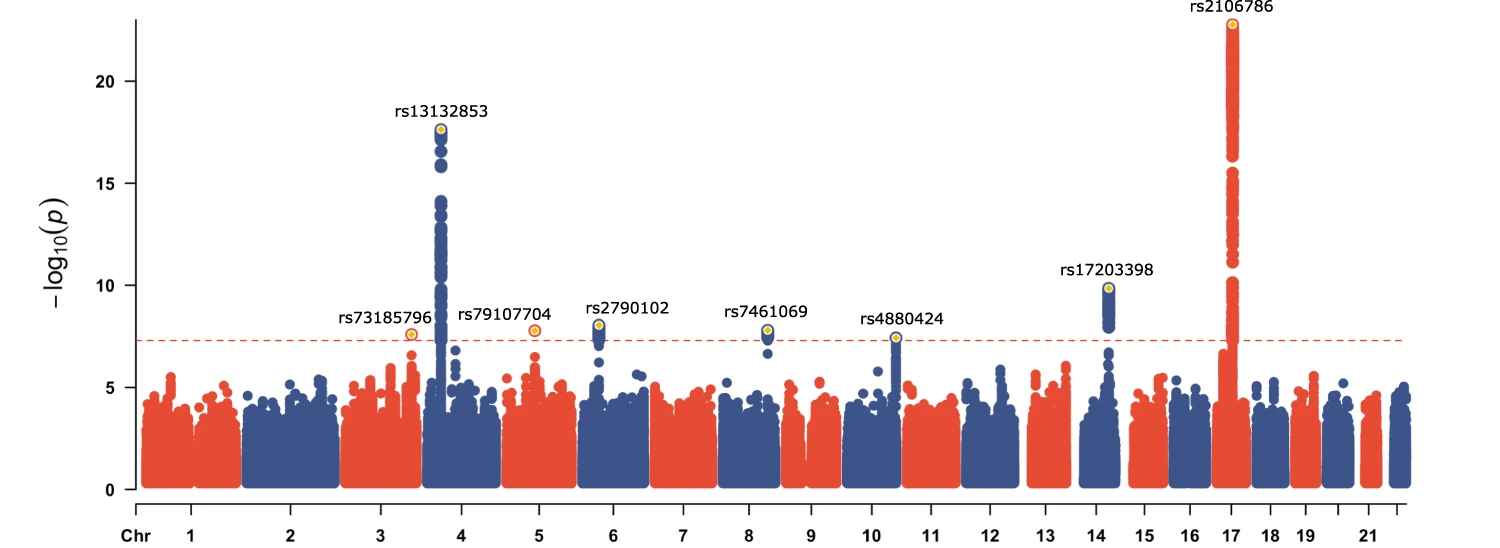
\includegraphics[width=10cm]{data/gwas.png}
			};
		\end{tikzpicture}
	\end{frame}

	\begin{frame}{AI i hjerneforskning: Genetikk, hjernealder og psykiatri}
		\centering
		\begin{tikzpicture}
			\node[fill=white, draw=black] {
				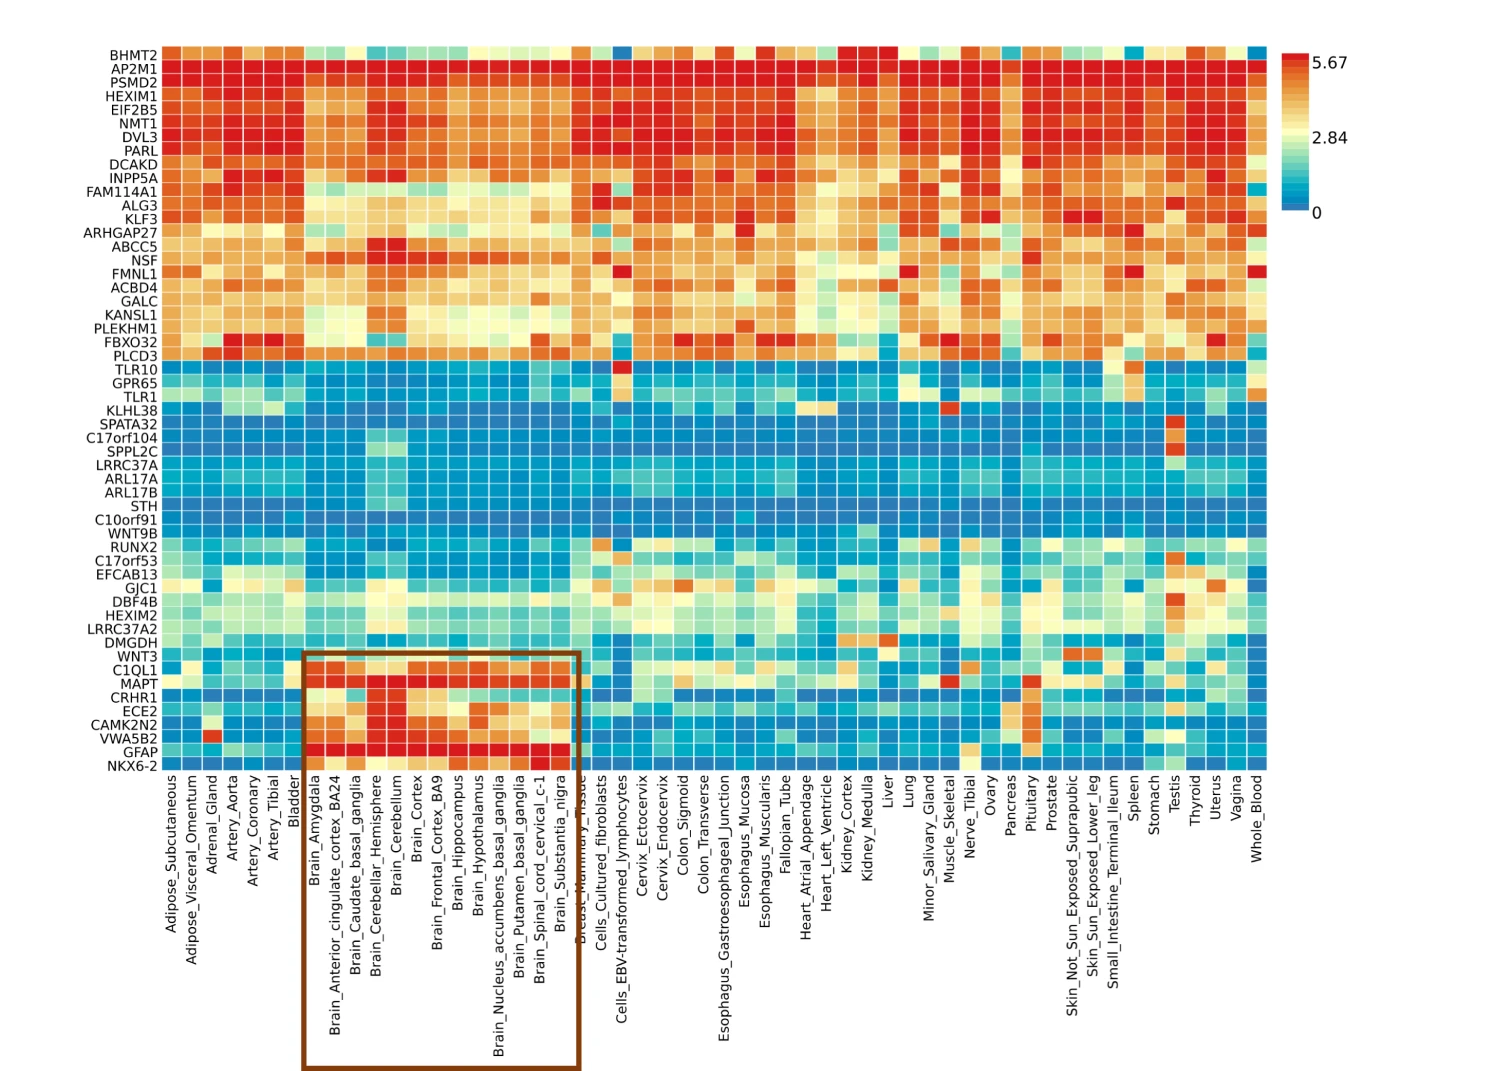
\includegraphics[width=8cm]{data/genes.png}
			};
		\end{tikzpicture}
	\end{frame}

	\begin{frame}{AI i hjerneforskning: Genetikk, hjernealder og psykiatri}
		\centering
		\begin{tikzpicture}
			\node[fill=white, draw=black] {
				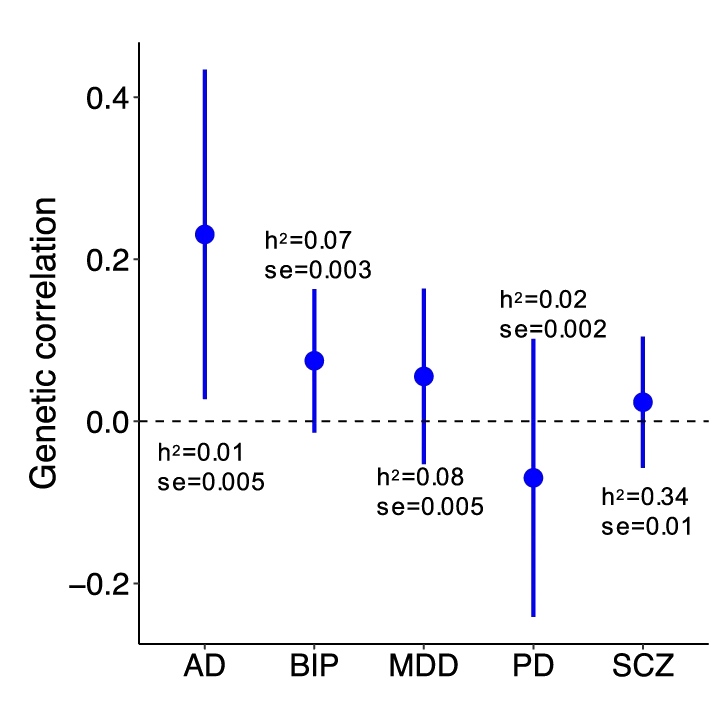
\includegraphics[width=6cm]{data/polygenic.png}
			};
		\end{tikzpicture}
	\end{frame}

	\begin{frame}{AI i hjerneforskning: Genetikk, hjernealder og psykiatri}
		\centering
		\begin{tikzpicture}
			\node[fill=white, draw=black] {
				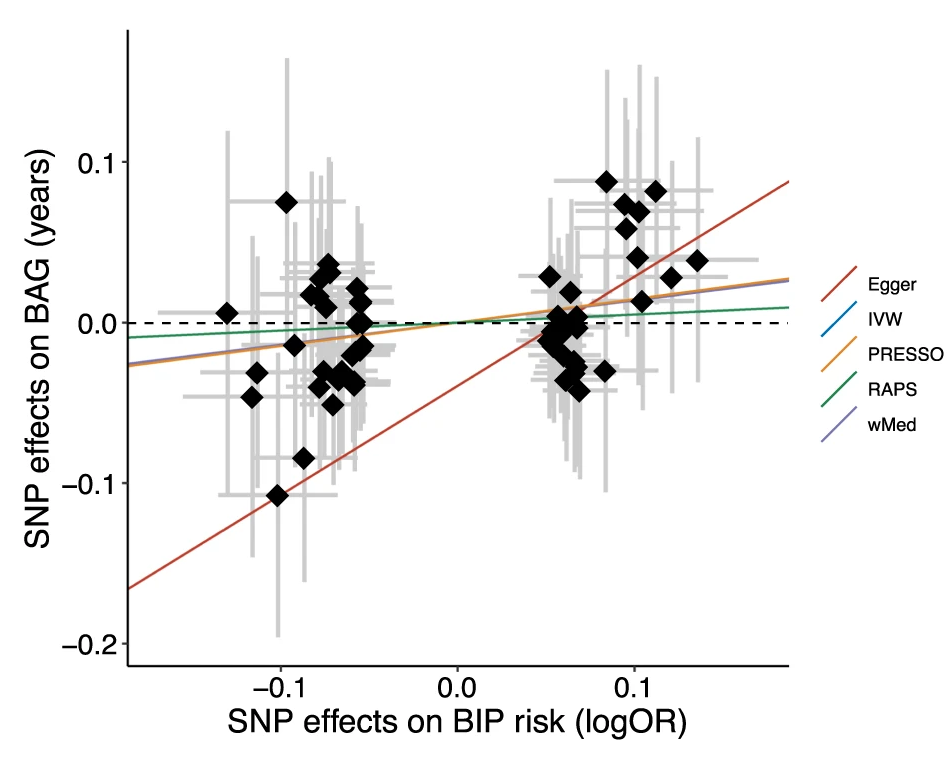
\includegraphics[width=7cm]{data/causal.png}
			};
		\end{tikzpicture}
	\end{frame}

	\begin{frame}{AI i hjerneforskning: Hjernealder}
		\begin{enumerate}
			\item Hvordan henger hjernealder sammen med psykiske lidelser?
			\item[ ] \textcolor{red}{Foreløpig uklart}
			\item Hva er hjernealder egentlig?
		\end{enumerate}
	\end{frame}

    \definecolor{train-fill}{HTML}{0079FF}

    % XAI: ANNs
	\begin{frame}{AI i hjerneforskning: Forklarbarhet}
		\begin{tikzpicture}
			\newcommand{\nodesize}{8pt}
			\newcommand{\hsep}{24pt}
			\newcommand{\vsep}{12pt}

			\newcommand{\arrowwidth}{0.05cm}
			\newcommand{\innerarrow}{{Latex[length=0.1cm, width=0.15cm]}}

			\newcommand{\modellocation}[1]{($ (0, 0) + ####1 $)}

			\node[circle, inner sep=0pt, fill=none, outer sep=0pt, line width=0pt, draw=none] (n00) at \modellocation{(-3 * \hsep, 0)} {};
			\node[] at (-5.5, 1.5) {};
			\node[] at (5.1, -1.2) {};

			\draw[black, fill=gray!20] (n00.center) --
							($ (n00) + (0, 2*\vsep+0.5*\nodesize+2pt) $) --
							($ (n00) + (6*\hsep+0.5*\nodesize+2pt, 2*\vsep+0.5*\nodesize+2pt) $) --
							($ (n00) + (6*\hsep+0.5*\nodesize+2pt, -2*\vsep-0.5*\nodesize-2pt) $) --
							($ (n00) + (0, -2*\vsep-0.5*\nodesize-2pt) $) --
							(n00.center);


			\node[circle, draw=black, minimum size=\nodesize, inner sep=0pt, fill=gray, outer sep=0pt, line width=0pt, draw=gray] (n10) at \modellocation{(-2 * \hsep, 2 * \vsep)} {};
			\node[circle, minimum size=\nodesize, inner sep=0pt, fill=gray, outer sep=0pt, line width=0pt, draw=gray] (n11) at \modellocation{(-2 * \hsep, 1 * \vsep)} {};
			\node[circle, minimum size=\nodesize, inner sep=0pt, fill=gray, outer sep=0pt, line width=0pt, draw=gray] (n12) at \modellocation{(-2 * \hsep, 0)} {};
			\node[circle, minimum size=\nodesize, inner sep=0pt, fill=gray, outer sep=0pt, line width=0pt, draw=gray] (n13) at \modellocation{(-2 * \hsep, -1 * \vsep)} {};
			\node[circle, minimum size=\nodesize, inner sep=0pt, fill=gray, outer sep=0pt, line width=0pt, draw=gray] (n14) at \modellocation{(-2 * \hsep, -2 * \vsep)} {};

			\node[circle, minimum size=\nodesize, inner sep=0pt, fill=gray, outer sep=0pt, line width=0pt, draw=gray] (n20) at \modellocation{(-1 * \hsep, 1.5 * \vsep)} {};
			\node[circle, minimum size=\nodesize, inner sep=0pt, fill=gray, outer sep=0pt, line width=0pt, draw=gray] (n21) at \modellocation{(-1 * \hsep, 0.5 * \vsep)} {};
			\node[circle, minimum size=\nodesize, inner sep=0pt, fill=gray, outer sep=0pt, line width=0pt, draw=gray] (n22) at \modellocation{(-1 * \hsep, -0.5 * \vsep)} {};
			\node[circle, minimum size=\nodesize, inner sep=0pt, fill=gray, outer sep=0pt, line width=0pt, draw=gray] (n23) at \modellocation{(-1 * \hsep, -1.5 * \vsep)} {};

			\node[circle, minimum size=\nodesize, inner sep=0pt, fill=gray, outer sep=0pt, line width=0pt, draw=gray] (n30) at \modellocation{(0 * \hsep, 1.5 * \vsep)} {};
			\node[circle, minimum size=\nodesize, inner sep=0pt, fill=gray, outer sep=0pt, line width=0pt, draw=gray] (n31) at \modellocation{(0 * \hsep, 0.5 * \vsep)} {};
			\node[circle, minimum size=\nodesize, inner sep=0pt, fill=gray, outer sep=0pt, line width=0pt, draw=gray] (n32) at \modellocation{(0 * \hsep, -0.5 * \vsep)} {};
			\node[circle, minimum size=\nodesize, inner sep=0pt, fill=gray, outer sep=0pt, line width=0pt, draw=gray] (n33) at \modellocation{(0 * \hsep, -1.5 * \vsep)} {};

			\node[circle, minimum size=\nodesize, inner sep=0pt, fill=gray, outer sep=0pt, line width=0pt, draw=gray] (n40) at \modellocation{(1 * \hsep, 1*\vsep)} {};
			\node[circle, minimum size=\nodesize, inner sep=0pt, fill=gray, outer sep=0pt, line width=0pt, draw=gray] (n41) at \modellocation{(1 * \hsep, 0*\vsep)} {};
			\node[circle, minimum size=\nodesize, inner sep=0pt, fill=gray, outer sep=0pt, line width=0pt, draw=gray] (n42) at \modellocation{(1 * \hsep, -1*\vsep)} {};

			\node[circle, minimum size=\nodesize, inner sep=0pt, fill=gray, outer sep=0pt, line width=0pt, draw=gray] (n50) at \modellocation{(2 * \hsep, 1*\vsep)} {};
			\node[circle, minimum size=\nodesize, inner sep=0pt, fill=gray, outer sep=0pt, line width=0pt, draw=gray] (n51) at \modellocation{(2 * \hsep, 0*\vsep)} {};
			\node[circle, minimum size=\nodesize, inner sep=0pt, fill=gray, outer sep=0pt, line width=0pt, draw=gray] (n52) at \modellocation{(2 * \hsep, -1*\vsep)} {};

			\node[circle, minimum size=\nodesize, inner sep=0pt, fill=gray, outer sep=0pt, line width=0pt, draw=gray] (n60) at \modellocation{(3 * \hsep, 0)} {};

			\draw[
				color=gray!70,
				-\innerarrow,
				line width=\arrowwidth
			] (n00) to [out=20,in=200] (n10) {};
			\draw[
				color=gray!70,
				-\innerarrow,
				line width=\arrowwidth
			] (n00) to [out=10,in=190] (n11) {};
			\draw[
				color=gray!70,
				-\innerarrow,
				line width=\arrowwidth
			] (n00) to [out=0,in=180] (n12) {};
			\draw[
				color=gray!70,
				-\innerarrow,
				line width=\arrowwidth
			] (n00) to [out=-10,in=170] (n13) {};
			\draw[
				color=gray!70,
				-\innerarrow,
				line width=\arrowwidth
			] (n00) to [out=-20,in=160] (n14) {};

			\draw[
				color=gray!70,
				-\innerarrow,
				line width=\arrowwidth
			] (n10) to [out=-5,in=175] (n20) {};
			\draw[
				color=gray!70,
				-\innerarrow,
				line width=\arrowwidth
			] (n10) to [out=-15,in=165] (n21) {};
			\draw[
				color=gray!70,
				-\innerarrow,
				line width=\arrowwidth
			] (n10) to [out=-25,in=155] (n22) {};
			\draw[
				color=gray!70,
				-\innerarrow,
				line width=\arrowwidth
			] (n10) to [out=-35,in=145] (n23) {};

			\draw[
				color=gray!70,
				-\innerarrow,
				line width=\arrowwidth
			] (n11) to [out=5,in=185] (n20) {};
			\draw[
				color=gray!70,
				-\innerarrow,
				line width=\arrowwidth
			] (n11) to [out=-5,in=175] (n21) {};
			\draw[
				color=gray!70,
				-\innerarrow,
				line width=\arrowwidth
			] (n11) to [out=-15,in=165] (n22) {};
			\draw[
				color=gray!70,
				-\innerarrow,
				line width=\arrowwidth
			] (n11) to [out=-25,in=155] (n23) {};

			\draw[
				color=gray!70,
				-\innerarrow,
				line width=\arrowwidth
			] (n12) to [out=15,in=195] (n20) {};
			\draw[
				color=gray!70,
				-\innerarrow,
				line width=\arrowwidth
			] (n12) to [out=5,in=185] (n21) {};
			\draw[
				color=gray!70,
				-\innerarrow,
				line width=\arrowwidth
			] (n12) to [out=-5,in=175] (n22) {};
			\draw[
				color=gray!70,
				-\innerarrow,
				line width=\arrowwidth
			] (n12) to [out=-15,in=165] (n23) {};

			\draw[
				color=gray!70,
				-\innerarrow,
				line width=\arrowwidth
			] (n13) to [out=25,in=205] (n20) {};
			\draw[
				color=gray!70,
				-\innerarrow,
				line width=\arrowwidth
			] (n13) to [out=15,in=195] (n21) {};
			\draw[
				color=gray!70,
				-\innerarrow,
				line width=\arrowwidth
			] (n13) to [out=5,in=185] (n22) {};
			\draw[
				color=gray!70,
				-\innerarrow,
				line width=\arrowwidth
			] (n13) to [out=-5,in=175] (n23) {};

			\draw[
				color=gray!70,
				-\innerarrow,
				line width=\arrowwidth
			] (n14) to [out=35,in=215] (n20) {};
			\draw[
				color=gray!70,
				-\innerarrow,
				line width=\arrowwidth
			] (n14) to [out=25,in=205] (n21) {};
			\draw[
				color=gray!70,
				-\innerarrow,
				line width=\arrowwidth
			] (n14) to [out=15,in=195] (n22) {};
			\draw[
				color=gray!70,
				-\innerarrow,
				line width=\arrowwidth
			] (n14) to [out=5,in=185] (n23) {};

			\draw[
				color=gray!70,
				-\innerarrow,
				line width=\arrowwidth
			] (n20) to [out=0,in=180] (n30) {};
			\draw[
				color=gray!70,
				-\innerarrow,
				line width=\arrowwidth
			] (n20) to [out=-10,in=170] (n31) {};
			\draw[
				color=gray!70,
				-\innerarrow,
				line width=\arrowwidth
			] (n20) to [out=-20,in=160] (n32) {};
			\draw[
				color=gray!70,
				-\innerarrow,
				line width=\arrowwidth
			] (n20) to [out=-30,in=150] (n33) {};

			\draw[
				color=gray!70,
				-\innerarrow,
				line width=\arrowwidth
			] (n21) to [out=10,in=190] (n30) {};
			\draw[
				color=gray!70,
				-\innerarrow,
				line width=\arrowwidth
			] (n21) to [out=0,in=180] (n31) {};
			\draw[
				color=gray!70,
				-\innerarrow,
				line width=\arrowwidth
			] (n21) to [out=-10,in=170] (n32) {};
			\draw[
				color=gray!70,
				-\innerarrow,
				line width=\arrowwidth
			] (n21) to [out=-20,in=160] (n33) {};

			\draw[
				color=gray!70,
				-\innerarrow,
				line width=\arrowwidth
			] (n22) to [out=20,in=200] (n30) {};
			\draw[
				color=gray!70,
				-\innerarrow,
				line width=\arrowwidth
			] (n22) to [out=10,in=190] (n31) {};
			\draw[
				color=gray!70,
				-\innerarrow,
				line width=\arrowwidth
			] (n22) to [out=0,in=180] (n32) {};
			\draw[
				color=gray!70,
				-\innerarrow,
				line width=\arrowwidth
			] (n22) to [out=-10,in=170] (n33) {};

			\draw[
				color=gray!70,
				-\innerarrow,
				line width=\arrowwidth
			] (n23) to [out=30,in=210] (n30) {};
			\draw[
				color=gray!70,
				-\innerarrow,
				line width=\arrowwidth
			] (n23) to [out=20,in=200] (n31) {};
			\draw[
				color=gray!70,
				-\innerarrow,
				line width=\arrowwidth
			] (n23) to [out=10,in=190] (n32) {};
			\draw[
				color=gray!70,
				-\innerarrow,
				line width=\arrowwidth
			] (n23) to [out=0,in=180] (n33) {};

			\draw[
				color=gray!70,
				-\innerarrow,
				line width=\arrowwidth
			] (n30) to [out=-5,in=175] (n40) {};
			\draw[
				color=gray!70,
				-\innerarrow,
				line width=\arrowwidth
			] (n30) to [out=-15,in=165] (n41) {};
			\draw[
				color=gray!70,
				-\innerarrow,
				line width=\arrowwidth
			] (n30) to [out=-25,in=155] (n42) {};

			\draw[
				color=gray!70,
				-\innerarrow,
				line width=\arrowwidth
			] (n31) to [out=5,in=185] (n40) {};
			\draw[
				color=gray!70,
				-\innerarrow,
				line width=\arrowwidth
			] (n31) to [out=-5,in=175] (n41) {};
			\draw[
				color=gray!70,
				-\innerarrow,
				line width=\arrowwidth
			] (n31) to [out=-15,in=165] (n42) {};

			\draw[
				color=gray!70,
				-\innerarrow,
				line width=\arrowwidth
			] (n32) to [out=15,in=195] (n40) {};
			\draw[
				color=gray!70,
				-\innerarrow,
				line width=\arrowwidth
			] (n32) to [out=5,in=185] (n41) {};
			\draw[
				color=gray!70,
				-\innerarrow,
				line width=\arrowwidth
			] (n32) to [out=-5,in=175] (n42) {};

			\draw[
				color=gray!70,
				-\innerarrow,
				line width=\arrowwidth
			] (n33) to [out=25,in=205] (n40) {};
			\draw[
				color=gray!70,
				-\innerarrow,
				line width=\arrowwidth
			] (n33) to [out=15,in=195] (n41) {};
			\draw[
				color=gray!70,
				-\innerarrow,
				line width=\arrowwidth
			] (n33) to [out=5,in=185] (n42) {};

			\draw[
				color=gray!70,
				-\innerarrow,
				line width=\arrowwidth
			] (n40) to [out=0,in=180] (n50) {};
			\draw[
				color=gray!70,
				-\innerarrow,
				line width=\arrowwidth
			] (n40) to [out=-10,in=170] (n51) {};
			\draw[
				color=gray!70,
				-\innerarrow,
				line width=\arrowwidth
			] (n40) to [out=-20,in=160] (n52) {};

			\draw[
				color=gray!70,
				-\innerarrow,
				line width=\arrowwidth
			] (n41) to [out=10,in=190] (n50) {};
			\draw[
				color=gray!70,
				-\innerarrow,
				line width=\arrowwidth
			] (n41) to [out=0,in=180] (n51) {};
			\draw[
				color=gray!70,
				-\innerarrow,
				line width=\arrowwidth
			] (n41) to [out=-10,in=170] (n52) {};

			\draw[
				color=gray!70,
				-\innerarrow,
				line width=\arrowwidth
			] (n42) to [out=20,in=200] (n50) {};
			\draw[
				color=gray!70,
				-\innerarrow,
				line width=\arrowwidth
			] (n42) to [out=10,in=190] (n51) {};
			\draw[
				color=gray!70,
				-\innerarrow,
				line width=\arrowwidth
			] (n42) to [out=0,in=180] (n52) {};

			\draw[
				color=gray!70,
				-\innerarrow,
				line width=\arrowwidth,
			] (n50) to [out=-10,in=170] (n60) {};
			\draw[
				color=gray!70,
				-\innerarrow,
				line width=\arrowwidth,
			] (n51) to [out=0,in=180] (n60) {};
			\draw[
				color=gray!70,
				-\innerarrow,
				line width=\arrowwidth,
			] (n52) to [out=10,in=190] (n60) {};


			\node[] at ($ (n30) + (0, \vsep+0.75*\nodesize) $) {Konvolusjonelt nevralt nettverk};
		\end{tikzpicture}
	\end{frame}

    % XAI: ANNs
	\begin{frame}{AI i hjerneforskning: Forklarbarhet}
		\begin{tikzpicture}
			\newcommand{\nodesize}{8pt}
			\newcommand{\hsep}{24pt}
			\newcommand{\vsep}{12pt}

			\newcommand{\arrowwidth}{0.05cm}
			\newcommand{\innerarrow}{{Latex[length=0.1cm, width=0.15cm]}}

			\newcommand{\modellocation}[1]{($ (0, 0) + ####1 $)}

			\node[circle, inner sep=0pt, fill=none, outer sep=0pt, line width=0pt, draw=none] (n00) at \modellocation{(-3 * \hsep, 0)} {};
			\node[] at (-5.5, 1.5) {};
			\node[] at (5.1, -1.2) {};

			\draw[black, fill=gray!20] (n00.center) --
							($ (n00) + (0, 2*\vsep+0.5*\nodesize+2pt) $) --
							($ (n00) + (6*\hsep+0.5*\nodesize+2pt, 2*\vsep+0.5*\nodesize+2pt) $) --
							($ (n00) + (6*\hsep+0.5*\nodesize+2pt, -2*\vsep-0.5*\nodesize-2pt) $) --
							($ (n00) + (0, -2*\vsep-0.5*\nodesize-2pt) $) --
							(n00.center);


			\node[circle, draw=black, minimum size=\nodesize, inner sep=0pt, fill=gray, outer sep=0pt, line width=0pt, draw=gray] (n10) at \modellocation{(-2 * \hsep, 2 * \vsep)} {};
			\node[circle, minimum size=\nodesize, inner sep=0pt, fill=gray, outer sep=0pt, line width=0pt, draw=gray] (n11) at \modellocation{(-2 * \hsep, 1 * \vsep)} {};
			\node[circle, minimum size=\nodesize, inner sep=0pt, fill=gray, outer sep=0pt, line width=0pt, draw=gray] (n12) at \modellocation{(-2 * \hsep, 0)} {};
			\node[circle, minimum size=\nodesize, inner sep=0pt, fill=gray, outer sep=0pt, line width=0pt, draw=gray] (n13) at \modellocation{(-2 * \hsep, -1 * \vsep)} {};
			\node[circle, minimum size=\nodesize, inner sep=0pt, fill=gray, outer sep=0pt, line width=0pt, draw=gray] (n14) at \modellocation{(-2 * \hsep, -2 * \vsep)} {};

			\node[circle, minimum size=\nodesize, inner sep=0pt, fill=gray, outer sep=0pt, line width=0pt, draw=gray] (n20) at \modellocation{(-1 * \hsep, 1.5 * \vsep)} {};
			\node[circle, minimum size=\nodesize, inner sep=0pt, fill=gray, outer sep=0pt, line width=0pt, draw=gray] (n21) at \modellocation{(-1 * \hsep, 0.5 * \vsep)} {};
			\node[circle, minimum size=\nodesize, inner sep=0pt, fill=gray, outer sep=0pt, line width=0pt, draw=gray] (n22) at \modellocation{(-1 * \hsep, -0.5 * \vsep)} {};
			\node[circle, minimum size=\nodesize, inner sep=0pt, fill=gray, outer sep=0pt, line width=0pt, draw=gray] (n23) at \modellocation{(-1 * \hsep, -1.5 * \vsep)} {};

			\node[circle, minimum size=\nodesize, inner sep=0pt, fill=gray, outer sep=0pt, line width=0pt, draw=gray] (n30) at \modellocation{(0 * \hsep, 1.5 * \vsep)} {};
			\node[circle, minimum size=\nodesize, inner sep=0pt, fill=gray, outer sep=0pt, line width=0pt, draw=gray] (n31) at \modellocation{(0 * \hsep, 0.5 * \vsep)} {};
			\node[circle, minimum size=\nodesize, inner sep=0pt, fill=gray, outer sep=0pt, line width=0pt, draw=gray] (n32) at \modellocation{(0 * \hsep, -0.5 * \vsep)} {};
			\node[circle, minimum size=\nodesize, inner sep=0pt, fill=gray, outer sep=0pt, line width=0pt, draw=gray] (n33) at \modellocation{(0 * \hsep, -1.5 * \vsep)} {};

			\node[circle, minimum size=\nodesize, inner sep=0pt, fill=gray, outer sep=0pt, line width=0pt, draw=gray] (n40) at \modellocation{(1 * \hsep, 1*\vsep)} {};
			\node[circle, minimum size=\nodesize, inner sep=0pt, fill=gray, outer sep=0pt, line width=0pt, draw=gray] (n41) at \modellocation{(1 * \hsep, 0*\vsep)} {};
			\node[circle, minimum size=\nodesize, inner sep=0pt, fill=gray, outer sep=0pt, line width=0pt, draw=gray] (n42) at \modellocation{(1 * \hsep, -1*\vsep)} {};

			\node[circle, minimum size=\nodesize, inner sep=0pt, fill=gray, outer sep=0pt, line width=0pt, draw=gray] (n50) at \modellocation{(2 * \hsep, 1*\vsep)} {};
			\node[circle, minimum size=\nodesize, inner sep=0pt, fill=gray, outer sep=0pt, line width=0pt, draw=gray] (n51) at \modellocation{(2 * \hsep, 0*\vsep)} {};
			\node[circle, minimum size=\nodesize, inner sep=0pt, fill=gray, outer sep=0pt, line width=0pt, draw=gray] (n52) at \modellocation{(2 * \hsep, -1*\vsep)} {};

			\node[circle, minimum size=\nodesize, inner sep=0pt, fill=gray, outer sep=0pt, line width=0pt, draw=gray] (n60) at \modellocation{(3 * \hsep, 0)} {};

			\draw[
				color=gray!70,
				-\innerarrow,
				line width=\arrowwidth
			] (n00) to [out=20,in=200] (n10) {};
			\draw[
				color=gray!70,
				-\innerarrow,
				line width=\arrowwidth
			] (n00) to [out=10,in=190] (n11) {};
			\draw[
				color=gray!70,
				-\innerarrow,
				line width=\arrowwidth
			] (n00) to [out=0,in=180] (n12) {};
			\draw[
				color=gray!70,
				-\innerarrow,
				line width=\arrowwidth
			] (n00) to [out=-10,in=170] (n13) {};
			\draw[
				color=gray!70,
				-\innerarrow,
				line width=\arrowwidth
			] (n00) to [out=-20,in=160] (n14) {};

			\draw[
				color=gray!70,
				-\innerarrow,
				line width=\arrowwidth
			] (n10) to [out=-5,in=175] (n20) {};
			\draw[
				color=gray!70,
				-\innerarrow,
				line width=\arrowwidth
			] (n10) to [out=-15,in=165] (n21) {};
			\draw[
				color=gray!70,
				-\innerarrow,
				line width=\arrowwidth
			] (n10) to [out=-25,in=155] (n22) {};
			\draw[
				color=gray!70,
				-\innerarrow,
				line width=\arrowwidth
			] (n10) to [out=-35,in=145] (n23) {};

			\draw[
				color=gray!70,
				-\innerarrow,
				line width=\arrowwidth
			] (n11) to [out=5,in=185] (n20) {};
			\draw[
				color=gray!70,
				-\innerarrow,
				line width=\arrowwidth
			] (n11) to [out=-5,in=175] (n21) {};
			\draw[
				color=gray!70,
				-\innerarrow,
				line width=\arrowwidth
			] (n11) to [out=-15,in=165] (n22) {};
			\draw[
				color=gray!70,
				-\innerarrow,
				line width=\arrowwidth
			] (n11) to [out=-25,in=155] (n23) {};

			\draw[
				color=gray!70,
				-\innerarrow,
				line width=\arrowwidth
			] (n12) to [out=15,in=195] (n20) {};
			\draw[
				color=gray!70,
				-\innerarrow,
				line width=\arrowwidth
			] (n12) to [out=5,in=185] (n21) {};
			\draw[
				color=gray!70,
				-\innerarrow,
				line width=\arrowwidth
			] (n12) to [out=-5,in=175] (n22) {};
			\draw[
				color=gray!70,
				-\innerarrow,
				line width=\arrowwidth
			] (n12) to [out=-15,in=165] (n23) {};

			\draw[
				color=gray!70,
				-\innerarrow,
				line width=\arrowwidth
			] (n13) to [out=25,in=205] (n20) {};
			\draw[
				color=gray!70,
				-\innerarrow,
				line width=\arrowwidth
			] (n13) to [out=15,in=195] (n21) {};
			\draw[
				color=gray!70,
				-\innerarrow,
				line width=\arrowwidth
			] (n13) to [out=5,in=185] (n22) {};
			\draw[
				color=gray!70,
				-\innerarrow,
				line width=\arrowwidth
			] (n13) to [out=-5,in=175] (n23) {};

			\draw[
				color=gray!70,
				-\innerarrow,
				line width=\arrowwidth
			] (n14) to [out=35,in=215] (n20) {};
			\draw[
				color=gray!70,
				-\innerarrow,
				line width=\arrowwidth
			] (n14) to [out=25,in=205] (n21) {};
			\draw[
				color=gray!70,
				-\innerarrow,
				line width=\arrowwidth
			] (n14) to [out=15,in=195] (n22) {};
			\draw[
				color=gray!70,
				-\innerarrow,
				line width=\arrowwidth
			] (n14) to [out=5,in=185] (n23) {};

			\draw[
				color=gray!70,
				-\innerarrow,
				line width=\arrowwidth
			] (n20) to [out=0,in=180] (n30) {};
			\draw[
				color=gray!70,
				-\innerarrow,
				line width=\arrowwidth
			] (n20) to [out=-10,in=170] (n31) {};
			\draw[
				color=gray!70,
				-\innerarrow,
				line width=\arrowwidth
			] (n20) to [out=-20,in=160] (n32) {};
			\draw[
				color=gray!70,
				-\innerarrow,
				line width=\arrowwidth
			] (n20) to [out=-30,in=150] (n33) {};

			\draw[
				color=gray!70,
				-\innerarrow,
				line width=\arrowwidth
			] (n21) to [out=10,in=190] (n30) {};
			\draw[
				color=gray!70,
				-\innerarrow,
				line width=\arrowwidth
			] (n21) to [out=0,in=180] (n31) {};
			\draw[
				color=gray!70,
				-\innerarrow,
				line width=\arrowwidth
			] (n21) to [out=-10,in=170] (n32) {};
			\draw[
				color=gray!70,
				-\innerarrow,
				line width=\arrowwidth
			] (n21) to [out=-20,in=160] (n33) {};

			\draw[
				color=gray!70,
				-\innerarrow,
				line width=\arrowwidth
			] (n22) to [out=20,in=200] (n30) {};
			\draw[
				color=gray!70,
				-\innerarrow,
				line width=\arrowwidth
			] (n22) to [out=10,in=190] (n31) {};
			\draw[
				color=gray!70,
				-\innerarrow,
				line width=\arrowwidth
			] (n22) to [out=0,in=180] (n32) {};
			\draw[
				color=gray!70,
				-\innerarrow,
				line width=\arrowwidth
			] (n22) to [out=-10,in=170] (n33) {};

			\draw[
				color=gray!70,
				-\innerarrow,
				line width=\arrowwidth
			] (n23) to [out=30,in=210] (n30) {};
			\draw[
				color=gray!70,
				-\innerarrow,
				line width=\arrowwidth
			] (n23) to [out=20,in=200] (n31) {};
			\draw[
				color=gray!70,
				-\innerarrow,
				line width=\arrowwidth
			] (n23) to [out=10,in=190] (n32) {};
			\draw[
				color=gray!70,
				-\innerarrow,
				line width=\arrowwidth
			] (n23) to [out=0,in=180] (n33) {};

			\draw[
				color=gray!70,
				-\innerarrow,
				line width=\arrowwidth
			] (n30) to [out=-5,in=175] (n40) {};
			\draw[
				color=gray!70,
				-\innerarrow,
				line width=\arrowwidth
			] (n30) to [out=-15,in=165] (n41) {};
			\draw[
				color=gray!70,
				-\innerarrow,
				line width=\arrowwidth
			] (n30) to [out=-25,in=155] (n42) {};

			\draw[
				color=gray!70,
				-\innerarrow,
				line width=\arrowwidth
			] (n31) to [out=5,in=185] (n40) {};
			\draw[
				color=gray!70,
				-\innerarrow,
				line width=\arrowwidth
			] (n31) to [out=-5,in=175] (n41) {};
			\draw[
				color=gray!70,
				-\innerarrow,
				line width=\arrowwidth
			] (n31) to [out=-15,in=165] (n42) {};

			\draw[
				color=gray!70,
				-\innerarrow,
				line width=\arrowwidth
			] (n32) to [out=15,in=195] (n40) {};
			\draw[
				color=gray!70,
				-\innerarrow,
				line width=\arrowwidth
			] (n32) to [out=5,in=185] (n41) {};
			\draw[
				color=gray!70,
				-\innerarrow,
				line width=\arrowwidth
			] (n32) to [out=-5,in=175] (n42) {};

			\draw[
				color=gray!70,
				-\innerarrow,
				line width=\arrowwidth
			] (n33) to [out=25,in=205] (n40) {};
			\draw[
				color=gray!70,
				-\innerarrow,
				line width=\arrowwidth
			] (n33) to [out=15,in=195] (n41) {};
			\draw[
				color=gray!70,
				-\innerarrow,
				line width=\arrowwidth
			] (n33) to [out=5,in=185] (n42) {};

			\draw[
				color=gray!70,
				-\innerarrow,
				line width=\arrowwidth
			] (n40) to [out=0,in=180] (n50) {};
			\draw[
				color=gray!70,
				-\innerarrow,
				line width=\arrowwidth
			] (n40) to [out=-10,in=170] (n51) {};
			\draw[
				color=gray!70,
				-\innerarrow,
				line width=\arrowwidth
			] (n40) to [out=-20,in=160] (n52) {};

			\draw[
				color=gray!70,
				-\innerarrow,
				line width=\arrowwidth
			] (n41) to [out=10,in=190] (n50) {};
			\draw[
				color=gray!70,
				-\innerarrow,
				line width=\arrowwidth
			] (n41) to [out=0,in=180] (n51) {};
			\draw[
				color=gray!70,
				-\innerarrow,
				line width=\arrowwidth
			] (n41) to [out=-10,in=170] (n52) {};

			\draw[
				color=gray!70,
				-\innerarrow,
				line width=\arrowwidth
			] (n42) to [out=20,in=200] (n50) {};
			\draw[
				color=gray!70,
				-\innerarrow,
				line width=\arrowwidth
			] (n42) to [out=10,in=190] (n51) {};
			\draw[
				color=gray!70,
				-\innerarrow,
				line width=\arrowwidth
			] (n42) to [out=0,in=180] (n52) {};

			\draw[
				color=gray!70,
				-\innerarrow,
				line width=\arrowwidth,
			] (n50) to [out=-10,in=170] (n60) {};
			\draw[
				color=gray!70,
				-\innerarrow,
				line width=\arrowwidth,
			] (n51) to [out=0,in=180] (n60) {};
			\draw[
				color=gray!70,
				-\innerarrow,
				line width=\arrowwidth,
			] (n52) to [out=10,in=190] (n60) {};

			\node[inner sep=0pt, outer sep=0pt, draw=black] (input) at ($ (n00) - (2, 0) $) {
				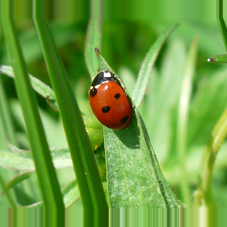
\includegraphics[height=2cm]{data/ladybug.png}
			};

			\newcommand{\outerarrow}{{Latex[length=0.2cm, width=0.3cm]}}
			\draw[-\outerarrow, line width=4pt, draw=gray] (input) to (n00);

			\node[] at ($ (n30) + (0, \vsep+0.75*\nodesize) $) {Konvolusjonelt nevralt nettverk};
		\end{tikzpicture}
	\end{frame}

	% XAI: Final layer
	\begin{frame}{AI i hjerneforskning: Forklarbarhet}
		\begin{tikzpicture}
			\newcommand{\nodesize}{8pt}
			\newcommand{\hsep}{24pt}
			\newcommand{\vsep}{12pt}

			\newcommand{\arrowwidth}{0.05cm}
			\newcommand{\innerarrow}{{Latex[length=0.1cm, width=0.15cm]}}

			\newcommand{\modellocation}[1]{($ (0, 0) + ####1 $)}

			\node[circle, inner sep=0pt, fill=none, outer sep=0pt, line width=0pt, draw=none] (n00) at \modellocation{(-3 * \hsep, 0)} {};
			\node[] at (-5.5, 1.5) {};
			\node[] at (5.1, -1.2) {};

			\draw[black, fill=gray!20] (n00.center) --
							($ (n00) + (0, 2*\vsep+0.5*\nodesize+2pt) $) --
							($ (n00) + (6*\hsep+0.5*\nodesize+2pt, 2*\vsep+0.5*\nodesize+2pt) $) --
							($ (n00) + (6*\hsep+0.5*\nodesize+2pt, -2*\vsep-0.5*\nodesize-2pt) $) --
							($ (n00) + (0, -2*\vsep-0.5*\nodesize-2pt) $) --
							(n00.center);


			\node[circle, draw=black, minimum size=\nodesize, inner sep=0pt, fill=train-fill!35, outer sep=0pt, line width=0pt, draw=train-fill!35] (n10) at \modellocation{(-2 * \hsep, 2 * \vsep)} {};
			\node[circle, minimum size=\nodesize, inner sep=0pt, fill=train-fill, outer sep=0pt, line width=0pt, draw=train-fill] (n11) at \modellocation{(-2 * \hsep, 1 * \vsep)} {};
			\node[circle, minimum size=\nodesize, inner sep=0pt, fill=train-fill!15, outer sep=0pt, line width=0pt, draw=train-fill!15] (n12) at \modellocation{(-2 * \hsep, 0)} {};
			\node[circle, minimum size=\nodesize, inner sep=0pt, fill=train-fill!85, outer sep=0pt, line width=0pt, draw=train-fill!85] (n13) at \modellocation{(-2 * \hsep, -1 * \vsep)} {};
			\node[circle, minimum size=\nodesize, inner sep=0pt, fill=train-fill!90, outer sep=0pt, line width=0pt, draw=train-fill!90] (n14) at \modellocation{(-2 * \hsep, -2 * \vsep)} {};

			\node[circle, minimum size=\nodesize, inner sep=0pt, fill=train-fill!55, outer sep=0pt, line width=0pt, draw=train-fill!55] (n20) at \modellocation{(-1 * \hsep, 1.5 * \vsep)} {};
			\node[circle, minimum size=\nodesize, inner sep=0pt, fill=train-fill!20, outer sep=0pt, line width=0pt, draw=train-fill!20] (n21) at \modellocation{(-1 * \hsep, 0.5 * \vsep)} {};
			\node[circle, minimum size=\nodesize, inner sep=0pt, fill=train-fill!90, outer sep=0pt, line width=0pt, draw=train-fill!50] (n22) at \modellocation{(-1 * \hsep, -0.5 * \vsep)} {};
			\node[circle, minimum size=\nodesize, inner sep=0pt, fill=train-fill!35, outer sep=0pt, line width=0pt, draw=train-fill!35] (n23) at \modellocation{(-1 * \hsep, -1.5 * \vsep)} {};

			\node[circle, minimum size=\nodesize, inner sep=0pt, fill=train-fill!95, outer sep=0pt, line width=0pt, draw=train-fill!65] (n30) at \modellocation{(0 * \hsep, 1.5 * \vsep)} {};
			\node[circle, minimum size=\nodesize, inner sep=0pt, fill=train-fill!20, outer sep=0pt, line width=0pt, draw=train-fill!20] (n31) at \modellocation{(0 * \hsep, 0.5 * \vsep)} {};
			\node[circle, minimum size=\nodesize, inner sep=0pt, fill=train-fill!90, outer sep=0pt, line width=0pt, draw=train-fill!90] (n32) at \modellocation{(0 * \hsep, -0.5 * \vsep)} {};
			\node[circle, minimum size=\nodesize, inner sep=0pt, fill=train-fill!80, outer sep=0pt, line width=0pt, draw=train-fill!80] (n33) at \modellocation{(0 * \hsep, -1.5 * \vsep)} {};

			\node[circle, minimum size=\nodesize, inner sep=0pt, fill=train-fill!50, outer sep=0pt, line width=0pt, draw=train-fill!50] (n40) at \modellocation{(1 * \hsep, 1*\vsep)} {};
			\node[circle, minimum size=\nodesize, inner sep=0pt, fill=train-fill!90, outer sep=0pt, line width=0pt, draw=train-fill!70] (n41) at \modellocation{(1 * \hsep, 0*\vsep)} {};
			\node[circle, minimum size=\nodesize, inner sep=0pt, fill=train-fill!70, outer sep=0pt, line width=0pt, draw=train-fill!30] (n42) at \modellocation{(1 * \hsep, -1*\vsep)} {};

			\node[circle, minimum size=\nodesize, inner sep=0pt, fill=train-fill, outer sep=0pt, line width=0pt, draw=train-fill] (n50) at \modellocation{(2 * \hsep, 1*\vsep)} {};
			\node[circle, minimum size=\nodesize, inner sep=0pt, fill=train-fill!70, outer sep=0pt, line width=0pt, draw=train-fill!70] (n51) at \modellocation{(2 * \hsep, 0*\vsep)} {};
			\node[circle, minimum size=\nodesize, inner sep=0pt, fill=train-fill!30, outer sep=0pt, line width=0pt, draw=train-fill!30] (n52) at \modellocation{(2 * \hsep, -1*\vsep)} {};

			\node[circle, minimum size=\nodesize, inner sep=0pt, fill=train-fill!80, outer sep=0pt, line width=0pt, draw=train-fill!65] (n60) at \modellocation{(3 * \hsep, 0)} {};

			\draw[
				color=train-fill!35,
				-\innerarrow,
				line width=\arrowwidth
			] (n00) to [out=20,in=200] (n10) {};
			\draw[
				color=train-fill,
				-\innerarrow,
				line width=\arrowwidth
			] (n00) to [out=10,in=190] (n11) {};
			\draw[
				color=train-fill!15,
				-\innerarrow,
				line width=\arrowwidth
			] (n00) to [out=0,in=180] (n12) {};
			\draw[
				color=train-fill!85,
				-\innerarrow,
				line width=\arrowwidth
			] (n00) to [out=-10,in=170] (n13) {};
			\draw[
				color=train-fill!90,
				-\innerarrow,
				line width=\arrowwidth
			] (n00) to [out=-20,in=160] (n14) {};

			\draw[
				color=train-fill!35,
				-\innerarrow,
				line width=\arrowwidth
			] (n10) to [out=-5,in=175] (n20) {};
			\draw[
				color=train-fill!10,
				-\innerarrow,
				line width=\arrowwidth
			] (n10) to [out=-15,in=165] (n21) {};
			\draw[
				color=train-fill!70,
				-\innerarrow,
				line width=\arrowwidth
			] (n10) to [out=-25,in=155] (n22) {};
			\draw[
				color=train-fill!50,
				-\innerarrow,
				line width=\arrowwidth
			] (n10) to [out=-35,in=145] (n23) {};

			\draw[
				color=train-fill!30,
				-\innerarrow,
				line width=\arrowwidth
			] (n11) to [out=5,in=185] (n20) {};
			\draw[
				color=train-fill!25,
				-\innerarrow,
				line width=\arrowwidth
			] (n11) to [out=-5,in=175] (n21) {};
			\draw[
				color=train-fill!95,
				-\innerarrow,
				line width=\arrowwidth
			] (n11) to [out=-15,in=165] (n22) {};
			\draw[
				color=train-fill!35,
				-\innerarrow,
				line width=\arrowwidth
			] (n11) to [out=-25,in=155] (n23) {};

			\draw[
				color=train-fill!70,
				-\innerarrow,
				line width=\arrowwidth
			] (n12) to [out=15,in=195] (n20) {};
			\draw[
				color=train-fill!20,
				-\innerarrow,
				line width=\arrowwidth
			] (n12) to [out=5,in=185] (n21) {};
			\draw[
				color=train-fill!80,
				-\innerarrow,
				line width=\arrowwidth
			] (n12) to [out=-5,in=175] (n22) {};
			\draw[
				color=train-fill,
				-\innerarrow,
				line width=\arrowwidth
			] (n12) to [out=-15,in=165] (n23) {};

			\draw[
				color=train-fill!40,
				-\innerarrow,
				line width=\arrowwidth
			] (n13) to [out=25,in=205] (n20) {};
			\draw[
				color=train-fill!35,
				-\innerarrow,
				line width=\arrowwidth
			] (n13) to [out=15,in=195] (n21) {};
			\draw[
				color=train-fill!20,
				-\innerarrow,
				line width=\arrowwidth
			] (n13) to [out=5,in=185] (n22) {};
			\draw[
				color=white,
				-\innerarrow,
				line width=\arrowwidth
			] (n13) to [out=-5,in=175] (n23) {};

			\draw[
				color=train-fill!40,
				-\innerarrow,
				line width=\arrowwidth
			] (n14) to [out=35,in=215] (n20) {};
			\draw[
				color=train-fill!85,
				-\innerarrow,
				line width=\arrowwidth
			] (n14) to [out=25,in=205] (n21) {};
			\draw[
				color=train-fill!35,
				-\innerarrow,
				line width=\arrowwidth
			] (n14) to [out=15,in=195] (n22) {};
			\draw[
				color=train-fill,
				-\innerarrow,
				line width=\arrowwidth
			] (n14) to [out=5,in=185] (n23) {};

			\draw[
				color=train-fill!85,
				-\innerarrow,
				line width=\arrowwidth
			] (n20) to [out=0,in=180] (n30) {};
			\draw[
				color=train-fill!50,
				-\innerarrow,
				line width=\arrowwidth
			] (n20) to [out=-10,in=170] (n31) {};
			\draw[
				color=train-fill!75,
				-\innerarrow,
				line width=\arrowwidth
			] (n20) to [out=-20,in=160] (n32) {};
			\draw[
				color=white,
				-\innerarrow,
				line width=\arrowwidth
			] (n20) to [out=-30,in=150] (n33) {};

			\draw[
				color=train-fill,
				-\innerarrow,
				line width=\arrowwidth
			] (n21) to [out=10,in=190] (n30) {};
			\draw[
				color=train-fill!30,
				-\innerarrow,
				line width=\arrowwidth
			] (n21) to [out=0,in=180] (n31) {};
			\draw[
				color=train-fill!25,
				-\innerarrow,
				line width=\arrowwidth
			] (n21) to [out=-10,in=170] (n32) {};
			\draw[
				color=white,
				-\innerarrow,
				line width=\arrowwidth
			] (n21) to [out=-20,in=160] (n33) {};

			\draw[
				color=train-fill!35,
				-\innerarrow,
				line width=\arrowwidth
			] (n22) to [out=20,in=200] (n30) {};
			\draw[
				color=train-fill!95,
				-\innerarrow,
				line width=\arrowwidth
			] (n22) to [out=10,in=190] (n31) {};
			\draw[
				color=train-fill!80,
				-\innerarrow,
				line width=\arrowwidth
			] (n22) to [out=0,in=180] (n32) {};
			\draw[
				color=white,
				-\innerarrow,
				line width=\arrowwidth
			] (n22) to [out=-10,in=170] (n33) {};

			\draw[
				color=train-fill!45,
				-\innerarrow,
				line width=\arrowwidth
			] (n23) to [out=30,in=210] (n30) {};
			\draw[
				color=train-fill!70,
				-\innerarrow,
				line width=\arrowwidth
			] (n23) to [out=20,in=200] (n31) {};
			\draw[
				color=train-fill!10,
				-\innerarrow,
				line width=\arrowwidth
			] (n23) to [out=10,in=190] (n32) {};
			\draw[
				color=train-fill!20,
				-\innerarrow,
				line width=\arrowwidth
			] (n23) to [out=0,in=180] (n33) {};

			\draw[
				color=train-fill!50,
				-\innerarrow,
				line width=\arrowwidth
			] (n30) to [out=-5,in=175] (n40) {};
			\draw[
				color=train-fill!30,
				-\innerarrow,
				line width=\arrowwidth
			] (n30) to [out=-15,in=165] (n41) {};
			\draw[
				color=train-fill,
				-\innerarrow,
				line width=\arrowwidth
			] (n30) to [out=-25,in=155] (n42) {};

			\draw[
				color=train-fill!45,
				-\innerarrow,
				line width=\arrowwidth
			] (n31) to [out=5,in=185] (n40) {};
			\draw[
				color=train-fill!90,
				-\innerarrow,
				line width=\arrowwidth
			] (n31) to [out=-5,in=175] (n41) {};
			\draw[
				color=train-fill!45,
				-\innerarrow,
				line width=\arrowwidth
			] (n31) to [out=-15,in=165] (n42) {};

			\draw[
				color=train-fill!15,
				-\innerarrow,
				line width=\arrowwidth
			] (n32) to [out=15,in=195] (n40) {};
			\draw[
				color=train-fill!70,
				-\innerarrow,
				line width=\arrowwidth
			] (n32) to [out=5,in=185] (n41) {};
			\draw[
				color=train-fill!50,
				-\innerarrow,
				line width=\arrowwidth
			] (n32) to [out=-5,in=175] (n42) {};

			\draw[
				color=train-fill!40,
				-\innerarrow,
				line width=\arrowwidth
			] (n33) to [out=25,in=205] (n40) {};
			\draw[
				color=train-fill!20,
				-\innerarrow,
				line width=\arrowwidth
			] (n33) to [out=15,in=195] (n41) {};
			\draw[
				color=train-fill!90,
				-\innerarrow,
				line width=\arrowwidth
			] (n33) to [out=5,in=185] (n42) {};

			\draw[
				color=train-fill!25,
				-\innerarrow,
				line width=\arrowwidth
			] (n40) to [out=0,in=180] (n50) {};
			\draw[
				color=train-fill!15,
				-\innerarrow,
				line width=\arrowwidth
			] (n40) to [out=-10,in=170] (n51) {};
			\draw[
				color=train-fill,
				-\innerarrow,
				line width=\arrowwidth
			] (n40) to [out=-20,in=160] (n52) {};

			\draw[
				color=train-fill!35,
				-\innerarrow,
				line width=\arrowwidth
			] (n41) to [out=10,in=190] (n50) {};
			\draw[
				color=train-fill!10,
				-\innerarrow,
				line width=\arrowwidth
			] (n41) to [out=0,in=180] (n51) {};
			\draw[
				color=train-fill!90,
				-\innerarrow,
				line width=\arrowwidth
			] (n41) to [out=-10,in=170] (n52) {};

			\draw[
				color=train-fill!50,
				-\innerarrow,
				line width=\arrowwidth
			] (n42) to [out=20,in=200] (n50) {};
			\draw[
				color=train-fill!40,
				-\innerarrow,
				line width=\arrowwidth
			] (n42) to [out=10,in=190] (n51) {};
			\draw[
				color=train-fill!20,
				-\innerarrow,
				line width=\arrowwidth
			] (n42) to [out=0,in=180] (n52) {};

			\draw[
				color=train-fill!80,
				-\innerarrow,
				line width=\arrowwidth,
			] (n50) to [out=-10,in=170] (n60) {};
			\draw[
				color=train-fill!90,
				-\innerarrow,
				line width=\arrowwidth,
			] (n51) to [out=0,in=180] (n60) {};
			\draw[
				color=train-fill!30,
				-\innerarrow,
				line width=\arrowwidth,
			] (n52) to [out=10,in=190] (n60) {};


			\node[] at ($ (n30) + (0, \vsep+0.75*\nodesize) $) {Konvolusjonelt nevralt nettverk};

			\node[inner sep=0pt, outer sep=0pt, draw=black] (input) at ($ (n00) - (2, 0) $) {
				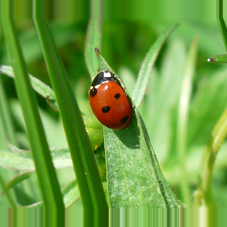
\includegraphics[height=2cm]{data/ladybug.png}
			};

			\newcommand{\outerarrow}{{Latex[length=0.2cm, width=0.3cm]}}
			\draw[-\outerarrow, line width=4pt, draw=gray] (input) to (n00);

		\end{tikzpicture}
	\end{frame}

    % XAI: Prediction
	\begin{frame}{AI i hjerneforskning: Forklarbarhet}
		\begin{tikzpicture}
			\newcommand{\nodesize}{8pt}
			\newcommand{\hsep}{24pt}
			\newcommand{\vsep}{12pt}

			\newcommand{\arrowwidth}{0.05cm}
			\newcommand{\innerarrow}{{Latex[length=0.1cm, width=0.15cm]}}

			\newcommand{\modellocation}[1]{($ (0, 0) + ####1 $)}

			\node[circle, inner sep=0pt, fill=none, outer sep=0pt, line width=0pt, draw=none] (n00) at \modellocation{(-3 * \hsep, 0)} {};
			\node[] at (-5.5, 1.5) {};
			\node[] at (5.1, -1.2) {};

			\draw[black, fill=gray!20] (n00.center) --
							($ (n00) + (0, 2*\vsep+0.5*\nodesize+2pt) $) --
							($ (n00) + (6*\hsep+0.5*\nodesize+2pt, 2*\vsep+0.5*\nodesize+2pt) $) --
							($ (n00) + (6*\hsep+0.5*\nodesize+2pt, -2*\vsep-0.5*\nodesize-2pt) $) --
							($ (n00) + (0, -2*\vsep-0.5*\nodesize-2pt) $) --
							(n00.center);


			\node[circle, draw=black, minimum size=\nodesize, inner sep=0pt, fill=train-fill!35, outer sep=0pt, line width=0pt, draw=train-fill!35] (n10) at \modellocation{(-2 * \hsep, 2 * \vsep)} {};
			\node[circle, minimum size=\nodesize, inner sep=0pt, fill=train-fill, outer sep=0pt, line width=0pt, draw=train-fill] (n11) at \modellocation{(-2 * \hsep, 1 * \vsep)} {};
			\node[circle, minimum size=\nodesize, inner sep=0pt, fill=train-fill!15, outer sep=0pt, line width=0pt, draw=train-fill!15] (n12) at \modellocation{(-2 * \hsep, 0)} {};
			\node[circle, minimum size=\nodesize, inner sep=0pt, fill=train-fill!85, outer sep=0pt, line width=0pt, draw=train-fill!85] (n13) at \modellocation{(-2 * \hsep, -1 * \vsep)} {};
			\node[circle, minimum size=\nodesize, inner sep=0pt, fill=train-fill!90, outer sep=0pt, line width=0pt, draw=train-fill!90] (n14) at \modellocation{(-2 * \hsep, -2 * \vsep)} {};

			\node[circle, minimum size=\nodesize, inner sep=0pt, fill=train-fill!55, outer sep=0pt, line width=0pt, draw=train-fill!55] (n20) at \modellocation{(-1 * \hsep, 1.5 * \vsep)} {};
			\node[circle, minimum size=\nodesize, inner sep=0pt, fill=train-fill!20, outer sep=0pt, line width=0pt, draw=train-fill!20] (n21) at \modellocation{(-1 * \hsep, 0.5 * \vsep)} {};
			\node[circle, minimum size=\nodesize, inner sep=0pt, fill=train-fill!90, outer sep=0pt, line width=0pt, draw=train-fill!50] (n22) at \modellocation{(-1 * \hsep, -0.5 * \vsep)} {};
			\node[circle, minimum size=\nodesize, inner sep=0pt, fill=train-fill!35, outer sep=0pt, line width=0pt, draw=train-fill!35] (n23) at \modellocation{(-1 * \hsep, -1.5 * \vsep)} {};

			\node[circle, minimum size=\nodesize, inner sep=0pt, fill=train-fill!95, outer sep=0pt, line width=0pt, draw=train-fill!65] (n30) at \modellocation{(0 * \hsep, 1.5 * \vsep)} {};
			\node[circle, minimum size=\nodesize, inner sep=0pt, fill=train-fill!20, outer sep=0pt, line width=0pt, draw=train-fill!20] (n31) at \modellocation{(0 * \hsep, 0.5 * \vsep)} {};
			\node[circle, minimum size=\nodesize, inner sep=0pt, fill=train-fill!90, outer sep=0pt, line width=0pt, draw=train-fill!90] (n32) at \modellocation{(0 * \hsep, -0.5 * \vsep)} {};
			\node[circle, minimum size=\nodesize, inner sep=0pt, fill=train-fill!80, outer sep=0pt, line width=0pt, draw=train-fill!80] (n33) at \modellocation{(0 * \hsep, -1.5 * \vsep)} {};

			\node[circle, minimum size=\nodesize, inner sep=0pt, fill=train-fill!50, outer sep=0pt, line width=0pt, draw=train-fill!50] (n40) at \modellocation{(1 * \hsep, 1*\vsep)} {};
			\node[circle, minimum size=\nodesize, inner sep=0pt, fill=train-fill!90, outer sep=0pt, line width=0pt, draw=train-fill!70] (n41) at \modellocation{(1 * \hsep, 0*\vsep)} {};
			\node[circle, minimum size=\nodesize, inner sep=0pt, fill=train-fill!70, outer sep=0pt, line width=0pt, draw=train-fill!30] (n42) at \modellocation{(1 * \hsep, -1*\vsep)} {};

			\node[circle, minimum size=\nodesize, inner sep=0pt, fill=train-fill, outer sep=0pt, line width=0pt, draw=train-fill] (n50) at \modellocation{(2 * \hsep, 1*\vsep)} {};
			\node[circle, minimum size=\nodesize, inner sep=0pt, fill=train-fill!70, outer sep=0pt, line width=0pt, draw=train-fill!70] (n51) at \modellocation{(2 * \hsep, 0*\vsep)} {};
			\node[circle, minimum size=\nodesize, inner sep=0pt, fill=train-fill!30, outer sep=0pt, line width=0pt, draw=train-fill!30] (n52) at \modellocation{(2 * \hsep, -1*\vsep)} {};

			\node[circle, minimum size=\nodesize, inner sep=0pt, fill=train-fill!80, outer sep=0pt, line width=0pt, draw=train-fill!65] (n60) at \modellocation{(3 * \hsep, 0)} {};

			\draw[
				color=train-fill!35,
				-\innerarrow,
				line width=\arrowwidth
			] (n00) to [out=20,in=200] (n10) {};
			\draw[
				color=train-fill,
				-\innerarrow,
				line width=\arrowwidth
			] (n00) to [out=10,in=190] (n11) {};
			\draw[
				color=train-fill!15,
				-\innerarrow,
				line width=\arrowwidth
			] (n00) to [out=0,in=180] (n12) {};
			\draw[
				color=train-fill!85,
				-\innerarrow,
				line width=\arrowwidth
			] (n00) to [out=-10,in=170] (n13) {};
			\draw[
				color=train-fill!90,
				-\innerarrow,
				line width=\arrowwidth
			] (n00) to [out=-20,in=160] (n14) {};

			\draw[
				color=train-fill!35,
				-\innerarrow,
				line width=\arrowwidth
			] (n10) to [out=-5,in=175] (n20) {};
			\draw[
				color=train-fill!10,
				-\innerarrow,
				line width=\arrowwidth
			] (n10) to [out=-15,in=165] (n21) {};
			\draw[
				color=train-fill!70,
				-\innerarrow,
				line width=\arrowwidth
			] (n10) to [out=-25,in=155] (n22) {};
			\draw[
				color=train-fill!50,
				-\innerarrow,
				line width=\arrowwidth
			] (n10) to [out=-35,in=145] (n23) {};

			\draw[
				color=train-fill!30,
				-\innerarrow,
				line width=\arrowwidth
			] (n11) to [out=5,in=185] (n20) {};
			\draw[
				color=train-fill!25,
				-\innerarrow,
				line width=\arrowwidth
			] (n11) to [out=-5,in=175] (n21) {};
			\draw[
				color=train-fill!95,
				-\innerarrow,
				line width=\arrowwidth
			] (n11) to [out=-15,in=165] (n22) {};
			\draw[
				color=train-fill!35,
				-\innerarrow,
				line width=\arrowwidth
			] (n11) to [out=-25,in=155] (n23) {};

			\draw[
				color=train-fill!70,
				-\innerarrow,
				line width=\arrowwidth
			] (n12) to [out=15,in=195] (n20) {};
			\draw[
				color=train-fill!20,
				-\innerarrow,
				line width=\arrowwidth
			] (n12) to [out=5,in=185] (n21) {};
			\draw[
				color=train-fill!80,
				-\innerarrow,
				line width=\arrowwidth
			] (n12) to [out=-5,in=175] (n22) {};
			\draw[
				color=train-fill,
				-\innerarrow,
				line width=\arrowwidth
			] (n12) to [out=-15,in=165] (n23) {};

			\draw[
				color=train-fill!40,
				-\innerarrow,
				line width=\arrowwidth
			] (n13) to [out=25,in=205] (n20) {};
			\draw[
				color=train-fill!35,
				-\innerarrow,
				line width=\arrowwidth
			] (n13) to [out=15,in=195] (n21) {};
			\draw[
				color=train-fill!20,
				-\innerarrow,
				line width=\arrowwidth
			] (n13) to [out=5,in=185] (n22) {};
			\draw[
				color=white,
				-\innerarrow,
				line width=\arrowwidth
			] (n13) to [out=-5,in=175] (n23) {};

			\draw[
				color=train-fill!40,
				-\innerarrow,
				line width=\arrowwidth
			] (n14) to [out=35,in=215] (n20) {};
			\draw[
				color=train-fill!85,
				-\innerarrow,
				line width=\arrowwidth
			] (n14) to [out=25,in=205] (n21) {};
			\draw[
				color=train-fill!35,
				-\innerarrow,
				line width=\arrowwidth
			] (n14) to [out=15,in=195] (n22) {};
			\draw[
				color=train-fill,
				-\innerarrow,
				line width=\arrowwidth
			] (n14) to [out=5,in=185] (n23) {};

			\draw[
				color=train-fill!85,
				-\innerarrow,
				line width=\arrowwidth
			] (n20) to [out=0,in=180] (n30) {};
			\draw[
				color=train-fill!50,
				-\innerarrow,
				line width=\arrowwidth
			] (n20) to [out=-10,in=170] (n31) {};
			\draw[
				color=train-fill!75,
				-\innerarrow,
				line width=\arrowwidth
			] (n20) to [out=-20,in=160] (n32) {};
			\draw[
				color=white,
				-\innerarrow,
				line width=\arrowwidth
			] (n20) to [out=-30,in=150] (n33) {};

			\draw[
				color=train-fill,
				-\innerarrow,
				line width=\arrowwidth
			] (n21) to [out=10,in=190] (n30) {};
			\draw[
				color=train-fill!30,
				-\innerarrow,
				line width=\arrowwidth
			] (n21) to [out=0,in=180] (n31) {};
			\draw[
				color=train-fill!25,
				-\innerarrow,
				line width=\arrowwidth
			] (n21) to [out=-10,in=170] (n32) {};
			\draw[
				color=white,
				-\innerarrow,
				line width=\arrowwidth
			] (n21) to [out=-20,in=160] (n33) {};

			\draw[
				color=train-fill!35,
				-\innerarrow,
				line width=\arrowwidth
			] (n22) to [out=20,in=200] (n30) {};
			\draw[
				color=train-fill!95,
				-\innerarrow,
				line width=\arrowwidth
			] (n22) to [out=10,in=190] (n31) {};
			\draw[
				color=train-fill!80,
				-\innerarrow,
				line width=\arrowwidth
			] (n22) to [out=0,in=180] (n32) {};
			\draw[
				color=white,
				-\innerarrow,
				line width=\arrowwidth
			] (n22) to [out=-10,in=170] (n33) {};

			\draw[
				color=train-fill!45,
				-\innerarrow,
				line width=\arrowwidth
			] (n23) to [out=30,in=210] (n30) {};
			\draw[
				color=train-fill!70,
				-\innerarrow,
				line width=\arrowwidth
			] (n23) to [out=20,in=200] (n31) {};
			\draw[
				color=train-fill!10,
				-\innerarrow,
				line width=\arrowwidth
			] (n23) to [out=10,in=190] (n32) {};
			\draw[
				color=train-fill!20,
				-\innerarrow,
				line width=\arrowwidth
			] (n23) to [out=0,in=180] (n33) {};

			\draw[
				color=train-fill!50,
				-\innerarrow,
				line width=\arrowwidth
			] (n30) to [out=-5,in=175] (n40) {};
			\draw[
				color=train-fill!30,
				-\innerarrow,
				line width=\arrowwidth
			] (n30) to [out=-15,in=165] (n41) {};
			\draw[
				color=train-fill,
				-\innerarrow,
				line width=\arrowwidth
			] (n30) to [out=-25,in=155] (n42) {};

			\draw[
				color=train-fill!45,
				-\innerarrow,
				line width=\arrowwidth
			] (n31) to [out=5,in=185] (n40) {};
			\draw[
				color=train-fill!90,
				-\innerarrow,
				line width=\arrowwidth
			] (n31) to [out=-5,in=175] (n41) {};
			\draw[
				color=train-fill!45,
				-\innerarrow,
				line width=\arrowwidth
			] (n31) to [out=-15,in=165] (n42) {};

			\draw[
				color=train-fill!15,
				-\innerarrow,
				line width=\arrowwidth
			] (n32) to [out=15,in=195] (n40) {};
			\draw[
				color=train-fill!70,
				-\innerarrow,
				line width=\arrowwidth
			] (n32) to [out=5,in=185] (n41) {};
			\draw[
				color=train-fill!50,
				-\innerarrow,
				line width=\arrowwidth
			] (n32) to [out=-5,in=175] (n42) {};

			\draw[
				color=train-fill!40,
				-\innerarrow,
				line width=\arrowwidth
			] (n33) to [out=25,in=205] (n40) {};
			\draw[
				color=train-fill!20,
				-\innerarrow,
				line width=\arrowwidth
			] (n33) to [out=15,in=195] (n41) {};
			\draw[
				color=train-fill!90,
				-\innerarrow,
				line width=\arrowwidth
			] (n33) to [out=5,in=185] (n42) {};

			\draw[
				color=train-fill!25,
				-\innerarrow,
				line width=\arrowwidth
			] (n40) to [out=0,in=180] (n50) {};
			\draw[
				color=train-fill!15,
				-\innerarrow,
				line width=\arrowwidth
			] (n40) to [out=-10,in=170] (n51) {};
			\draw[
				color=train-fill,
				-\innerarrow,
				line width=\arrowwidth
			] (n40) to [out=-20,in=160] (n52) {};

			\draw[
				color=train-fill!35,
				-\innerarrow,
				line width=\arrowwidth
			] (n41) to [out=10,in=190] (n50) {};
			\draw[
				color=train-fill!10,
				-\innerarrow,
				line width=\arrowwidth
			] (n41) to [out=0,in=180] (n51) {};
			\draw[
				color=train-fill!90,
				-\innerarrow,
				line width=\arrowwidth
			] (n41) to [out=-10,in=170] (n52) {};

			\draw[
				color=train-fill!50,
				-\innerarrow,
				line width=\arrowwidth
			] (n42) to [out=20,in=200] (n50) {};
			\draw[
				color=train-fill!40,
				-\innerarrow,
				line width=\arrowwidth
			] (n42) to [out=10,in=190] (n51) {};
			\draw[
				color=train-fill!20,
				-\innerarrow,
				line width=\arrowwidth
			] (n42) to [out=0,in=180] (n52) {};

			\draw[
				color=train-fill!80,
				-\innerarrow,
				line width=\arrowwidth,
			] (n50) to [out=-10,in=170] (n60) {};
			\draw[
				color=train-fill!90,
				-\innerarrow,
				line width=\arrowwidth,
			] (n51) to [out=0,in=180] (n60) {};
			\draw[
				color=train-fill!30,
				-\innerarrow,
				line width=\arrowwidth,
			] (n52) to [out=10,in=190] (n60) {};


			\node[] at ($ (n30) + (0, \vsep+0.75*\nodesize) $) {Konvolusjonelt nevralt nettverk};

			\node[inner sep=0pt, outer sep=0pt, draw=black] (input) at ($ (n00) - (2, 0) $) {
				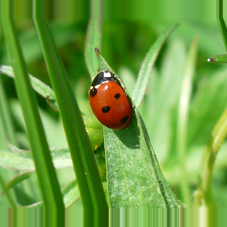
\includegraphics[height=2cm]{data/ladybug.png}
			};
			\node[] (output) at ($ (n60) + (2, 0) $) {
				"marihøne"
			};

			\newcommand{\outerarrow}{{Latex[length=0.2cm, width=0.3cm]}}
			\draw[-\outerarrow, line width=4pt, draw=gray] (input) to (n00);
			\draw[-\outerarrow, line width=4pt, draw=gray] ($ (n60.east) + (0.076, 0) $) to (output);


		\end{tikzpicture}
	\end{frame}

    % XAI: Heatmap
	\begin{frame}{AI i hjerneforskning: Forklarbarhet}
		\begin{tikzpicture}
			\newcommand{\nodesize}{8pt}
			\newcommand{\hsep}{24pt}
			\newcommand{\vsep}{12pt}

			\newcommand{\arrowwidth}{0.05cm}
			\newcommand{\innerarrow}{{Latex[length=0.1cm, width=0.15cm]}}

			\newcommand{\lrplocation}[1]{($ (0, 0) + ####1 $)}

			\colorlet{lrp-fill}{red}
			\colorlet{predict-fill}{blue}

			\node[circle, inner sep=0pt, fill=none, outer sep=0pt, line width=0pt, draw=none] (n00) at \lrplocation{(-3 * \hsep, 0)} {};
			\node[] at (-5.5, 1.5) {};
			\node[] at (5.1, -1.2) {};

			\draw[black, fill=gray!20] (n00.center) --
							($ (n00) + (0, 2*\vsep+0.5*\nodesize+2pt) $) --
							($ (n00) + (6*\hsep+0.5*\nodesize+2pt, 2*\vsep+0.5*\nodesize+2pt) $) --
							($ (n00) + (6*\hsep+0.5*\nodesize+2pt, -2*\vsep-0.5*\nodesize-2pt) $) --
							($ (n00) + (0, -2*\vsep-0.5*\nodesize-2pt) $) --
							(n00.center);


			\node[circle, inner sep=0pt, fill=none, outer sep=0pt, line width=0pt, draw=none] (n00) at \lrplocation{(-3 * \hsep, 0)} {};

			\node[circle, minimum size=\nodesize, inner sep=0pt, fill={rgb:black,5;orange,1}, outer sep=0pt, line width=0pt, draw={rgb:black,5;orange,1}] (n10) at \lrplocation{(-2 * \hsep, 2 * \vsep)} {};
			\node[circle, minimum size=\nodesize, inner sep=0pt, fill={rgb:black,3;red,1}, outer sep=0pt, line width=0pt, draw={rgb:black,3;red,1}] (n11) at \lrplocation{(-2 * \hsep, 1 * \vsep)} {};
			\node[circle, minimum size=\nodesize, inner sep=0pt, fill=yellow, outer sep=0pt, line width=0pt, draw=yellow] (n12) at \lrplocation{(-2 * \hsep, 0)} {};
			\node[circle, minimum size=\nodesize, inner sep=0pt, fill=black, outer sep=0pt, line width=0pt, draw=black] (n13) at \lrplocation{(-2 * \hsep, -1 * \vsep)} {};
			\node[circle, minimum size=\nodesize, inner sep=0pt, fill=red, outer sep=0pt, line width=0pt, draw=red] (n14) at \lrplocation{(-2 * \hsep, -2 * \vsep)} {};

			\node[circle, minimum size=\nodesize, inner sep=0pt, fill={rgb:black,5;white,2;orange,1}, outer sep=0pt, line width=0pt, draw={rgb:black,5;white,2;orange,1}] (n20) at \lrplocation{(-1 * \hsep, 1.5 * \vsep)} {};
			\node[circle, minimum size=\nodesize, inner sep=0pt, fill={rgb:red,10;yellow,6}, outer sep=0pt, line width=0pt, draw={rgb:red,10;yellow,4}] (n21) at \lrplocation{(-1 * \hsep, 0.5 * \vsep)} {};
			\node[circle, minimum size=\nodesize, inner sep=0pt, fill={rgb:red,10;yellow,1}, outer sep=0pt, line width=0pt, draw={rgb:red,10;yellow,1}] (n22) at \lrplocation{(-1 * \hsep, -0.5 * \vsep)} {};
			\node[circle, minimum size=\nodesize, inner sep=0pt, fill={rgb:black,10;red,2}, outer sep=0pt, line width=0pt, draw={rgb:black,10;red,2}] (n23) at \lrplocation{(-1 * \hsep, -1.5 * \vsep)} {};

			\node[circle, minimum size=\nodesize, inner sep=0pt, fill={rgb:red,3;orange,2}, outer sep=0pt, line width=0pt, draw={rgb:red,3;orange,1}] (n30) at \lrplocation{(0 * \hsep, 1.5 * \vsep)} {};
			\node[circle, minimum size=\nodesize, inner sep=0pt, fill={rgb:yellow,3;orange,1}, outer sep=0pt, line width=0pt, draw={rgb:yellow,3;orange,1}] (n31) at \lrplocation{(0 * \hsep, 0.5 * \vsep)} {};
			\node[circle, minimum size=\nodesize, inner sep=0pt, fill={rgb:black,10;white,5;red,1}, outer sep=0pt, line width=0pt, draw={rgb:black,10;white,5;red,1}] (n32) at \lrplocation{(0 * \hsep, -0.5 * \vsep)} {};
			\node[circle, minimum size=\nodesize, inner sep=0pt, fill={rgb:gray,5;red,1}, outer sep=0pt, line width=0pt, draw={rgb:gray,5;red,1}] (n33) at \lrplocation{(0 * \hsep, -1.5 * \vsep)} {};

			\node[circle, minimum size=\nodesize, inner sep=0pt, fill={rgb:yellow,10;orange,1}, outer sep=0pt, line width=0pt, draw={rgb:yellow,10;orange,1}] (n40) at \lrplocation{(1 * \hsep, 1*\vsep)} {};
			\node[circle, minimum size=\nodesize, inner sep=0pt, fill={rgb:red,1}, outer sep=0pt, line width=0pt, draw={rgb:red,1}] (n41) at \lrplocation{(1 * \hsep, 0*\vsep)} {};
			\node[circle, minimum size=\nodesize, inner sep=0pt, fill={rgb:black,10;white,15;red,2}, outer sep=0pt, line width=0pt, draw={rgb:black,10;white,15;red,2}] (n42) at \lrplocation{(1 * \hsep, -1*\vsep)} {};

			\node[circle, minimum size=\nodesize, inner sep=0pt, fill={rgb:red,5;black,1;yellow,2}, outer sep=0pt, line width=0pt, draw={rgb:red,5;black,1;yellow,2}] (n50) at \lrplocation{(2 * \hsep, 1*\vsep)} {};
			\node[circle, minimum size=\nodesize, inner sep=0pt, fill={rgb:gray,5;red,1}, outer sep=0pt, line width=0pt, draw={rgb:gray,5;red,1}] (n51) at \lrplocation{(2 * \hsep, 0*\vsep)} {};
			\node[circle, minimum size=\nodesize, inner sep=0pt, fill={rgb:yellow,5;orange,1}, outer sep=0pt, line width=0pt, draw={rgb:yellow,5;orange,1}] (n52) at \lrplocation{(2 * \hsep, -1*\vsep)} {};

			\node[circle, minimum size=\nodesize, inner sep=0pt, fill={rgb:orange,7;yellow,4;black,1}, outer sep=0pt, line width=0pt, draw={rgb:orange,7;yellow,4;black,1}] (n60) at \lrplocation{(3 * \hsep, 0)} {};

			\draw[
				color={rgb:black,5;orange,1},
				\innerarrow-,
				line width=\arrowwidth
			] (n00) to [out=20,in=200] (n10) {};
			\draw[
				color={rgb:black,3;red,1},
				\innerarrow-,
				line width=\arrowwidth
			] (n00) to [out=10,in=190] (n11) {};
			\draw[
				color=yellow,
				\innerarrow-,
				line width=\arrowwidth
			] (n00) to [out=0,in=180] (n12) {};
			\draw[
				color=black,
				\innerarrow-,
				line width=\arrowwidth
			] (n00) to [out=-10,in=170] (n13) {};
			\draw[
				color=red,
				\innerarrow-,
				line width=\arrowwidth
			] (n00) to [out=-20,in=160] (n14) {};

			\draw[
				color={rgb:black,5;white,1;orange,1},
				\innerarrow-,
				line width=\arrowwidth
			] (n10) to [out=-5,in=175] (n20) {};
			\draw[
				color={rgb:black,3;orange,1},
				\innerarrow-,
				line width=\arrowwidth
			] (n10) to [out=-15,in=165] (n21) {};
			\draw[
				color={rgb:black,4;red,2;yellow,1},
				\innerarrow-,
				line width=\arrowwidth
			] (n10) to [out=-25,in=155] (n22) {};
			\draw[
				color={rgb:black,3;red,1},
				\innerarrow-,
				line width=\arrowwidth
			] (n10) to [out=-35,in=145] (n23) {};

			\draw[
				color={rgb:black,10;orange,2},
				\innerarrow-,
				line width=\arrowwidth
			] (n11) to [out=5,in=185] (n20) {};
			\draw[
				color={rgb:black,3;orange,1},
				\innerarrow-,
				line width=\arrowwidth
			] (n11) to [out=-5,in=175] (n21) {};
			\draw[
				color={rgb:black,3;red,1},
				\innerarrow-,
				line width=\arrowwidth
			] (n11) to [out=-15,in=165] (n22) {};
			\draw[
				color={rgb:black,10;red,1},
				\innerarrow-,
				line width=\arrowwidth
			] (n11) to [out=-25,in=155] (n23) {};

			\draw[
				color={rgb:black,5;orange,3},
				\innerarrow-,
				line width=\arrowwidth
			] (n12) to [out=15,in=195] (n20) {};
			\draw[
				color={rgb:red,3;yellow,5},
				\innerarrow-,
				line width=\arrowwidth
			] (n12) to [out=5,in=185] (n21) {};
			\draw[
				color={rgb:red,5;yellow,3},
				\innerarrow-,
				line width=\arrowwidth
			] (n12) to [out=-5,in=175] (n22) {};
			\draw[
				color={rgb:black,5;orange,2},
				\innerarrow-,
				line width=\arrowwidth
			] (n12) to [out=-15,in=165] (n23) {};

			\draw[
				color={rgb:black,5;red,1},
				\innerarrow-,
				line width=\arrowwidth
			] (n13) to [out=25,in=205] (n20) {};
			\draw[
				color={rgb:black,5;orange,2},
				\innerarrow-,
				line width=\arrowwidth
			] (n13) to [out=15,in=195] (n21) {};
			\draw[
				color={rgb:black,5;red,3},
				\innerarrow-,
				line width=\arrowwidth
			] (n13) to [out=5,in=185] (n22) {};
			\draw[
				color=black,
				\innerarrow-,
				line width=\arrowwidth
			] (n13) to [out=-5,in=175] (n23) {};

			\draw[
				color={rgb:black,5;orange,2},
				\innerarrow-,
				line width=\arrowwidth
			] (n14) to [out=35,in=215] (n20) {};
			\draw[
				color={rgb:red,3;orange,1},
				\innerarrow-,
				line width=\arrowwidth
			] (n14) to [out=25,in=205] (n21) {};
			\draw[
				color={rgb:red,5;yellow,2},
				\innerarrow-,
				line width=\arrowwidth
			] (n14) to [out=15,in=195] (n22) {};
			\draw[
				color={rgb:black,5;red,3},
				\innerarrow-,
				line width=\arrowwidth
			] (n14) to [out=5,in=185] (n23) {};

			\draw[
				color={rgb:black,1;red,1},
				\innerarrow-,
				line width=\arrowwidth
			] (n20) to [out=0,in=180] (n30) {};
			\draw[
				color={rgb:black,3;orange,1},
				\innerarrow-,
				line width=\arrowwidth
			] (n20) to [out=-10,in=170] (n31) {};
			\draw[
				color={rgb:black,10;red,1},
				\innerarrow-,
				line width=\arrowwidth
			] (n20) to [out=-20,in=160] (n32) {};
			\draw[
				color={rgb:black,5;red,1},
				\innerarrow-,
				line width=\arrowwidth
			] (n20) to [out=-30,in=150] (n33) {};

			\draw[
				color={rgb:orange,5;red,2},
				\innerarrow-,
				line width=\arrowwidth
			] (n21) to [out=10,in=190] (n30) {};
			\draw[
				color={rgb:yellow,10;orange,4},
				\innerarrow-,
				line width=\arrowwidth
			] (n21) to [out=0,in=180] (n31) {};
			\draw[
				color={rgb:black,2;red,1},
				\innerarrow-,
				line width=\arrowwidth
			] (n21) to [out=-10,in=170] (n32) {};
			\draw[
				color={rgb:black,1;orange,2;red,1},
				\innerarrow-,
				line width=\arrowwidth
			] (n21) to [out=-20,in=160] (n33) {};

			\draw[
				color={rgb:red,2;orange,1},
				\innerarrow-,
				line width=\arrowwidth
			] (n22) to [out=20,in=200] (n30) {};
			\draw[
				color={rgb:yellow,2;orange,1},
				\innerarrow-,
				line width=\arrowwidth
			] (n22) to [out=10,in=190] (n31) {};
			\draw[
				color={rgb:black,2;red,2},
				\innerarrow-,
				line width=\arrowwidth
			] (n22) to [out=0,in=180] (n32) {};
			\draw[
				color={rgb:black,2;orange,1},
				\innerarrow-,
				line width=\arrowwidth
			] (n22) to [out=-10,in=170] (n33) {};

			\draw[
				color={rgb:black,4;red,2},
				\innerarrow-,
				line width=\arrowwidth
			] (n23) to [out=30,in=210] (n30) {};
			\draw[
				color={rgb:orange,2;black,1},
				\innerarrow-,
				line width=\arrowwidth
			] (n23) to [out=20,in=200] (n31) {};
			\draw[
				color={rgb:black,5;orange,1},
				\innerarrow-,
				line width=\arrowwidth
			] (n23) to [out=10,in=190] (n32) {};
			\draw[
				color={rgb:black,5;red,2},
				\innerarrow-,
				line width=\arrowwidth
			] (n23) to [out=0,in=180] (n33) {};

			\draw[
				color={rgb:orange,3;red,1},
				\innerarrow-,
				line width=\arrowwidth
			] (n30) to [out=-5,in=175] (n40) {};
			\draw[
				color={rgb:gray,1;orange,1;red,2},
				\innerarrow-,
				line width=\arrowwidth
			] (n30) to [out=-15,in=165] (n41) {};
			\draw[
				color={rgb:orange,2;black,2;white,1},
				\innerarrow-,
				line width=\arrowwidth
			] (n30) to [out=-25,in=155] (n42) {};

			\draw[
				color={rgb:yellow,5;orange,1},
				\innerarrow-,
				line width=\arrowwidth
			] (n31) to [out=5,in=185] (n40) {};
			\draw[
				color={rgb:red,3;orange,1},
				\innerarrow-,
				line width=\arrowwidth
			] (n31) to [out=-5,in=175] (n41) {};
			\draw[
				color={rgb:gray,1;red,2},
				\innerarrow-,
				line width=\arrowwidth
			] (n31) to [out=-15,in=165] (n42) {};

			\draw[
				color={rgb:gray,3;orange,1},
				\innerarrow-,
				line width=\arrowwidth
			] (n32) to [out=15,in=195] (n40) {};
			\draw[
				color={rgb:gray,1;red,1},
				\innerarrow-,
				line width=\arrowwidth
			] (n32) to [out=5,in=185] (n41) {};
			\draw[
				color={rgb:gray,1},
				\innerarrow-,
				line width=\arrowwidth
			] (n32) to [out=-5,in=175] (n42) {};

			\draw[
				color={rgb:gray,2;orange,3},
				\innerarrow-,
				line width=\arrowwidth
			] (n33) to [out=25,in=205] (n40) {};
			\draw[
				color={rgb:gray,1;orange,1},
				\innerarrow-,
				line width=\arrowwidth
			] (n33) to [out=15,in=195] (n41) {};
			\draw[
				color={rgb:gray,3;red,1},
				\innerarrow-,
				line width=\arrowwidth
			] (n33) to [out=5,in=185] (n42) {};

			\draw[
				color={rgb:red,3;yellow,1},
				\innerarrow-,
				line width=\arrowwidth
			] (n40) to [out=0,in=180] (n50) {};
			\draw[
				color={rgb:gray,2;orange,1},
				\innerarrow-,
				line width=\arrowwidth
			] (n40) to [out=-10,in=170] (n51) {};
			\draw[
				color={rgb:yellow,10;orange,1},
				\innerarrow-,
				line width=\arrowwidth
			] (n40) to [out=-20,in=160] (n52) {};

			\draw[
				color={rgb:red,5;black,1;yellow,2},
				\innerarrow-,
				line width=\arrowwidth
			] (n41) to [out=10,in=190] (n50) {};
			\draw[
				color={rgb:gray,7;orange,3},
				\innerarrow-,
				line width=\arrowwidth
			] (n41) to [out=0,in=180] (n51) {};
			\draw[
				color={rgb:yellow,1;orange,2},
				\innerarrow-,
				line width=\arrowwidth
			] (n41) to [out=-10,in=170] (n52) {};

			\draw[
				color={rgb:gray,7;orange,2},
				\innerarrow-,
				line width=\arrowwidth
			] (n42) to [out=20,in=200] (n50) {};
			\draw[
				color={rgb:gray,5;red,1},
				\innerarrow-,
				line width=\arrowwidth
			] (n42) to [out=10,in=190] (n51) {};
			\draw[
				color={rgb:gray,5;red,1;black,2},
				\innerarrow-,
				line width=\arrowwidth
			] (n42) to [out=0,in=180] (n52) {};

			\draw[
				color={rgb:red,5;black,1;yellow,2},
				\innerarrow-,
				line width=\arrowwidth
			] (n50) to [out=-10,in=170] (n60) {};
			\draw[
				color={rgb:gray,5;red,1},
				\innerarrow-,
				line width=\arrowwidth
			] (n51) to [out=0,in=180] (n60) {};
			\draw[
				color={rgb:yellow,5;orange,1},
				\innerarrow-,
				line width=\arrowwidth
			] (n52) to [out=10,in=190] (n60) {};


			\node[] at ($ (n30) + (0, \vsep+0.75*\nodesize) $) {Konvolusjonelt nevralt nettverk};

			\node[inner sep=0pt, outer sep=0pt, draw=black] (input) at ($ (n00) - (2, 0) $) {
				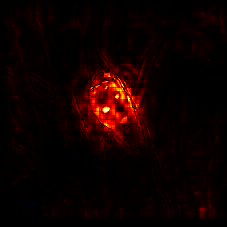
\includegraphics[height=2cm]{data/ladybug_explanation.png}
			};
			\node[] (output) at ($ (n60) + (2, 0) $) {
				"marihøne"
			};

			\newcommand{\outerarrow}{{Latex[length=0.2cm, width=0.3cm]}}
			\draw[\outerarrow-, line width=4pt, draw=gray] (input) to (n00);
			\draw[\outerarrow-, line width=4pt, draw=gray] ($ (n60.east) + (0.076, 0) $) to (output);


		\end{tikzpicture}
	\end{frame}

	\definecolor{cases-default}{HTML}{EB5353}
	\definecolor{controls-default}{HTML}{0079FF}
	\definecolor{healthy-default}{HTML}{36AE7C}

    \begin{frame}{AI i hjerneforskning: Forklarbarhet} % Full dataset

		\def\xmin{46}
		\def\xmax{99}
		\def\ymin{-1.4}
		\def\ymax{1.2}

		\centering
		\vfill
		\begin{tikzpicture}
            \begin{axis}[
                width=\textwidth,
                height=0.45\textwidth,
                xmin=\xmin,
                xmax=\xmax,
                ymin=-1.6,
                ymax=\ymax,
                xtick={55,60,65,70,75,80,85,90,95},
				axis lines=center,
				axis y line=none,
				clip=false
            ]
                \addplot[name path=zero, draw=none] coordinates {(47,0) (97,0)};
                \addplot[name path=fcases, draw=cases-default, very thick] table [x=x, y=F-cases, col sep=comma]{data/dementia_full.csv};\label{trace:cases}
                 \addplot[fill=cases-default, opacity=0.2] fill between [of=zero and fcases];
                 \addplot[name path=fcontrols, draw=controls-default, very thick] table [x=x, y=F-controls, col sep=comma]{data/dementia_full.csv};\label{trace:controls}
                 \addplot[fill=controls-default, opacity=0.2] fill between [of=zero and fcontrols];
                 \addplot[name path=mcases, draw=cases-default, very thick] table [x=x,y expr=\thisrow{M-cases} * -1, col sep=comma]{data/dementia_full.csv};
                 \addplot[fill=cases-default, opacity=0.2] fill between [of=zero and mcases];
                 \addplot[name path=mcontrols, draw=controls-default, very thick] table [x=x,y expr=\thisrow{M-controls} * -1, col sep=comma]{data/dementia_full.csv};
                 \addplot[fill=controls-default, opacity=0.2] fill between [of=zero and mcontrols];
                 \node[anchor=south west] at (axis cs: 46, 0.07) {\textbf{KVINNER}};
                 \node[anchor=north west] at (axis cs: 46, -0.07) {\textbf{MENN}};
                 \node[anchor=south, align=center] (n) at (axis cs: 72.5,-1.6) {n=1708};
                 \node[anchor=north] at ($(n.south) + (0,-2.5) $) {\ref{trace:controls} Friske\hspace{0.3cm}\ref{trace:cases} Pasienter};
            \end{axis}
        \end{tikzpicture}
		\vspace{-0.1cm}
		\vfill
	\end{frame}

    \begin{frame}{AI i hjerneforskning: Forklarbarhet} % Modelling
        \centering
        \vfill
		\begin{tikzpicture}[scale=0.9]
            \newcommand{\mrivsep}{0.52}
			\newcommand{\mrihsep}{0.44}
			\def\plotwidth{11.68}

			\newcommand{\nodesize}{11pt}
			\newcommand{\hsep}{28pt}
			\newcommand{\vsep}{14pt}

			\newcommand{\arrowwidth}{0.05cm}
			\newcommand{\innerarrow}{{Latex[length=0.1cm, width=0.15cm]}}
			\newcommand{\outerarrow}{{Latex[length=0.2cm, width=0.3cm]}}

			\definecolor{cb-green}{HTML}{4dac93}
			\definecolor{cb-blue}{HTML}{3594d6}
			\definecolor{outercolor}{RGB}{128, 128, 128}
			\colorlet{train-fill}{cb-blue}

			\newcommand{\patientlocation}[1]{($ (1, -1.6) + ####1 $)}
			\newcommand{\controllocation}[1]{($ (1, -2.8) + ####1 $)}
			\newcommand{\modellocation}[1]{($ (0.5 * \plotwidth, -2.2) + ####1 $)}

            \node[thick, draw=green, inner sep=0pt] (p0) at (2, -1.1) {
                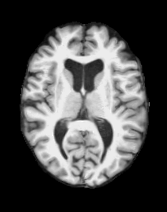
\includegraphics[width=0.6cm]{data/samples/control_0.png}
            };

            \node[thick, draw=green, inner sep=0pt] (p0) at (1.1, -0.7) {
                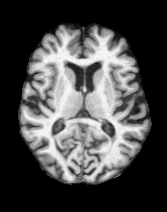
\includegraphics[width=0.6cm]{data/samples/control_1.png}
            };

            \node[thick, draw=green, inner sep=0pt] (p0) at (1.25, -1.9) {
                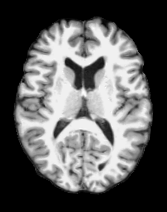
\includegraphics[width=0.6cm]{data/samples/control_2.png}
            };

            \node[thick, draw=green, inner sep=0pt] (p0) at (0.3, -1.4) {
                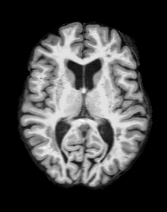
\includegraphics[width=0.6cm]{data/samples/control_3.png}
            };

            \node[thick, draw=red, inner sep=0pt] (p0) at (2.2, -3.1) {
                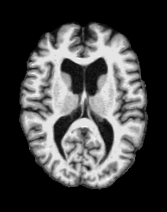
\includegraphics[width=0.6cm]{data/samples/control_4.png}
            };

            \node[thick, draw=red, inner sep=0pt] (p0) at (1.4, -3.2) {
                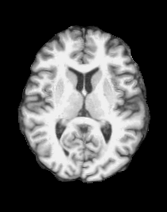
\includegraphics[width=0.6cm]{data/samples/control_5.png}
            };

            \node[thick, draw=red, inner sep=0pt] (p0) at (0.4, -2.7) {
                \includegraphics[width=0.6cm]{data/samples/dementia_0.png}
            };

			\node[circle, inner sep=0pt, fill=none, outer sep=0pt, line width=0pt, draw=none] (n00) at \modellocation{(-3 * \hsep, 0)} {};

			\node[circle, minimum size=\nodesize, inner sep=0pt, fill=train-fill!35, outer sep=0pt, line width=0pt, draw=train-fill!35] (n10) at \modellocation{(-2 * \hsep, 2 * \vsep)} {};
			\node[circle, minimum size=\nodesize, inner sep=0pt, fill=train-fill, outer sep=0pt, line width=0pt, draw=train-fill] (n11) at \modellocation{(-2 * \hsep, 1 * \vsep)} {};
			\node[circle, minimum size=\nodesize, inner sep=0pt, fill=train-fill!15, outer sep=0pt, line width=0pt, draw=train-fill!15] (n12) at \modellocation{(-2 * \hsep, 0)} {};
			\node[circle, minimum size=\nodesize, inner sep=0pt, fill=train-fill!85, outer sep=0pt, line width=0pt, draw=train-fill!85] (n13) at \modellocation{(-2 * \hsep, -1 * \vsep)} {};
			\node[circle, minimum size=\nodesize, inner sep=0pt, fill=train-fill!90, outer sep=0pt, line width=0pt, draw=train-fill!90] (n14) at \modellocation{(-2 * \hsep, -2 * \vsep)} {};

			\node[circle, minimum size=\nodesize, inner sep=0pt, fill=train-fill!55, outer sep=0pt, line width=0pt, draw=train-fill!55] (n20) at \modellocation{(-1 * \hsep, 1.5 * \vsep)} {};
			\node[circle, minimum size=\nodesize, inner sep=0pt, fill=train-fill!20, outer sep=0pt, line width=0pt, draw=train-fill!20] (n21) at \modellocation{(-1 * \hsep, 0.5 * \vsep)} {};
			\node[circle, minimum size=\nodesize, inner sep=0pt, fill=train-fill!90, outer sep=0pt, line width=0pt, draw=train-fill!50] (n22) at \modellocation{(-1 * \hsep, -0.5 * \vsep)} {};
			\node[circle, minimum size=\nodesize, inner sep=0pt, fill=train-fill!35, outer sep=0pt, line width=0pt, draw=train-fill!35] (n23) at \modellocation{(-1 * \hsep, -1.5 * \vsep)} {};

			\node[circle, minimum size=\nodesize, inner sep=0pt, fill=train-fill!95, outer sep=0pt, line width=0pt, draw=train-fill!65] (n30) at \modellocation{(0 * \hsep, 1.5 * \vsep)} {};
			\node[circle, minimum size=\nodesize, inner sep=0pt, fill=train-fill!20, outer sep=0pt, line width=0pt, draw=train-fill!20] (n31) at \modellocation{(0 * \hsep, 0.5 * \vsep)} {};
			\node[circle, minimum size=\nodesize, inner sep=0pt, fill=train-fill!90, outer sep=0pt, line width=0pt, draw=train-fill!90] (n32) at \modellocation{(0 * \hsep, -0.5 * \vsep)} {};
			\node[circle, minimum size=\nodesize, inner sep=0pt, fill=train-fill!80, outer sep=0pt, line width=0pt, draw=train-fill!80] (n33) at \modellocation{(0 * \hsep, -1.5 * \vsep)} {};

			\node[circle, minimum size=\nodesize, inner sep=0pt, fill=train-fill!50, outer sep=0pt, line width=0pt, draw=train-fill!50] (n40) at \modellocation{(1 * \hsep, 1*\vsep)} {};
			\node[circle, minimum size=\nodesize, inner sep=0pt, fill=train-fill!90, outer sep=0pt, line width=0pt, draw=train-fill!70] (n41) at \modellocation{(1 * \hsep, 0*\vsep)} {};
			\node[circle, minimum size=\nodesize, inner sep=0pt, fill=train-fill!70, outer sep=0pt, line width=0pt, draw=train-fill!30] (n42) at \modellocation{(1 * \hsep, -1*\vsep)} {};

			\node[circle, minimum size=\nodesize, inner sep=0pt, fill=train-fill, outer sep=0pt, line width=0pt, draw=train-fill] (n50) at \modellocation{(2 * \hsep, 1*\vsep)} {};
			\node[circle, minimum size=\nodesize, inner sep=0pt, fill=train-fill!70, outer sep=0pt, line width=0pt, draw=train-fill!70] (n51) at \modellocation{(2 * \hsep, 0*\vsep)} {};
			\node[circle, minimum size=\nodesize, inner sep=0pt, fill=train-fill!30, outer sep=0pt, line width=0pt, draw=train-fill!30] (n52) at \modellocation{(2 * \hsep, -1*\vsep)} {};

			\node[circle, minimum size=\nodesize, inner sep=0pt, fill=train-fill!80, outer sep=0pt, line width=0pt, draw=train-fill!65] (n60) at \modellocation{(3 * \hsep, 0)} {};

			\draw[
				color=train-fill!35,
				-\innerarrow,
				line width=\arrowwidth
			] (n00) to [out=20,in=200] (n10) {};
			\draw[
				color=train-fill,
				-\innerarrow,
				line width=\arrowwidth
			] (n00) to [out=10,in=190] (n11) {};
			\draw[
				color=train-fill!15,
				-\innerarrow,
				line width=\arrowwidth
			] (n00) to [out=0,in=180] (n12) {};
			\draw[
				color=train-fill!85,
				-\innerarrow,
				line width=\arrowwidth
			] (n00) to [out=-10,in=170] (n13) {};
			\draw[
				color=train-fill!90,
				-\innerarrow,
				line width=\arrowwidth
			] (n00) to [out=-20,in=160] (n14) {};

			\draw[
				color=train-fill!35,
				-\innerarrow,
				line width=\arrowwidth
			] (n10) to [out=-5,in=175] (n20) {};
			\draw[
				color=train-fill!10,
				-\innerarrow,
				line width=\arrowwidth
			] (n10) to [out=-15,in=165] (n21) {};
			\draw[
				color=train-fill!70,
				-\innerarrow,
				line width=\arrowwidth
			] (n10) to [out=-25,in=155] (n22) {};
			\draw[
				color=train-fill!50,
				-\innerarrow,
				line width=\arrowwidth
			] (n10) to [out=-35,in=145] (n23) {};

			\draw[
				color=train-fill!30,
				-\innerarrow,
				line width=\arrowwidth
			] (n11) to [out=5,in=185] (n20) {};
			\draw[
				color=train-fill!25,
				-\innerarrow,
				line width=\arrowwidth
			] (n11) to [out=-5,in=175] (n21) {};
			\draw[
				color=train-fill!95,
				-\innerarrow,
				line width=\arrowwidth
			] (n11) to [out=-15,in=165] (n22) {};
			\draw[
				color=train-fill!35,
				-\innerarrow,
				line width=\arrowwidth
			] (n11) to [out=-25,in=155] (n23) {};

			\draw[
				color=train-fill!70,
				-\innerarrow,
				line width=\arrowwidth
			] (n12) to [out=15,in=195] (n20) {};
			\draw[
				color=train-fill!20,
				-\innerarrow,
				line width=\arrowwidth
			] (n12) to [out=5,in=185] (n21) {};
			\draw[
				color=train-fill!80,
				-\innerarrow,
				line width=\arrowwidth
			] (n12) to [out=-5,in=175] (n22) {};
			\draw[
				color=train-fill,
				-\innerarrow,
				line width=\arrowwidth
			] (n12) to [out=-15,in=165] (n23) {};

			\draw[
				color=train-fill!40,
				-\innerarrow,
				line width=\arrowwidth
			] (n13) to [out=25,in=205] (n20) {};
			\draw[
				color=train-fill!35,
				-\innerarrow,
				line width=\arrowwidth
			] (n13) to [out=15,in=195] (n21) {};
			\draw[
				color=train-fill!20,
				-\innerarrow,
				line width=\arrowwidth
			] (n13) to [out=5,in=185] (n22) {};
			\draw[
				color=white,
				-\innerarrow,
				line width=\arrowwidth
			] (n13) to [out=-5,in=175] (n23) {};

			\draw[
				color=train-fill!40,
				-\innerarrow,
				line width=\arrowwidth
			] (n14) to [out=35,in=215] (n20) {};
			\draw[
				color=train-fill!85,
				-\innerarrow,
				line width=\arrowwidth
			] (n14) to [out=25,in=205] (n21) {};
			\draw[
				color=train-fill!35,
				-\innerarrow,
				line width=\arrowwidth
			] (n14) to [out=15,in=195] (n22) {};
			\draw[
				color=train-fill,
				-\innerarrow,
				line width=\arrowwidth
			] (n14) to [out=5,in=185] (n23) {};

			\draw[
				color=train-fill!85,
				-\innerarrow,
				line width=\arrowwidth
			] (n20) to [out=0,in=180] (n30) {};
			\draw[
				color=train-fill!50,
				-\innerarrow,
				line width=\arrowwidth
			] (n20) to [out=-10,in=170] (n31) {};
			\draw[
				color=train-fill!75,
				-\innerarrow,
				line width=\arrowwidth
			] (n20) to [out=-20,in=160] (n32) {};
			\draw[
				color=white,
				-\innerarrow,
				line width=\arrowwidth
			] (n20) to [out=-30,in=150] (n33) {};

			\draw[
				color=train-fill,
				-\innerarrow,
				line width=\arrowwidth
			] (n21) to [out=10,in=190] (n30) {};
			\draw[
				color=train-fill!30,
				-\innerarrow,
				line width=\arrowwidth
			] (n21) to [out=0,in=180] (n31) {};
			\draw[
				color=train-fill!25,
				-\innerarrow,
				line width=\arrowwidth
			] (n21) to [out=-10,in=170] (n32) {};
			\draw[
				color=white,
				-\innerarrow,
				line width=\arrowwidth
			] (n21) to [out=-20,in=160] (n33) {};

			\draw[
				color=train-fill!35,
				-\innerarrow,
				line width=\arrowwidth
			] (n22) to [out=20,in=200] (n30) {};
			\draw[
				color=train-fill!95,
				-\innerarrow,
				line width=\arrowwidth
			] (n22) to [out=10,in=190] (n31) {};
			\draw[
				color=train-fill!80,
				-\innerarrow,
				line width=\arrowwidth
			] (n22) to [out=0,in=180] (n32) {};
			\draw[
				color=white,
				-\innerarrow,
				line width=\arrowwidth
			] (n22) to [out=-10,in=170] (n33) {};

			\draw[
				color=train-fill!45,
				-\innerarrow,
				line width=\arrowwidth
			] (n23) to [out=30,in=210] (n30) {};
			\draw[
				color=train-fill!70,
				-\innerarrow,
				line width=\arrowwidth
			] (n23) to [out=20,in=200] (n31) {};
			\draw[
				color=train-fill!10,
				-\innerarrow,
				line width=\arrowwidth
			] (n23) to [out=10,in=190] (n32) {};
			\draw[
				color=train-fill!20,
				-\innerarrow,
				line width=\arrowwidth
			] (n23) to [out=0,in=180] (n33) {};

			\draw[
				color=train-fill!50,
				-\innerarrow,
				line width=\arrowwidth
			] (n30) to [out=-5,in=175] (n40) {};
			\draw[
				color=train-fill!30,
				-\innerarrow,
				line width=\arrowwidth
			] (n30) to [out=-15,in=165] (n41) {};
			\draw[
				color=train-fill,
				-\innerarrow,
				line width=\arrowwidth
			] (n30) to [out=-25,in=155] (n42) {};

			\draw[
				color=train-fill!45,
				-\innerarrow,
				line width=\arrowwidth
			] (n31) to [out=5,in=185] (n40) {};
			\draw[
				color=train-fill!90,
				-\innerarrow,
				line width=\arrowwidth
			] (n31) to [out=-5,in=175] (n41) {};
			\draw[
				color=train-fill!45,
				-\innerarrow,
				line width=\arrowwidth
			] (n31) to [out=-15,in=165] (n42) {};

			\draw[
				color=train-fill!15,
				-\innerarrow,
				line width=\arrowwidth
			] (n32) to [out=15,in=195] (n40) {};
			\draw[
				color=train-fill!70,
				-\innerarrow,
				line width=\arrowwidth
			] (n32) to [out=5,in=185] (n41) {};
			\draw[
				color=train-fill!50,
				-\innerarrow,
				line width=\arrowwidth
			] (n32) to [out=-5,in=175] (n42) {};

			\draw[
				color=train-fill!40,
				-\innerarrow,
				line width=\arrowwidth
			] (n33) to [out=25,in=205] (n40) {};
			\draw[
				color=train-fill!20,
				-\innerarrow,
				line width=\arrowwidth
			] (n33) to [out=15,in=195] (n41) {};
			\draw[
				color=train-fill!90,
				-\innerarrow,
				line width=\arrowwidth
			] (n33) to [out=5,in=185] (n42) {};

			\draw[
				color=train-fill!25,
				-\innerarrow,
				line width=\arrowwidth
			] (n40) to [out=0,in=180] (n50) {};
			\draw[
				color=train-fill!15,
				-\innerarrow,
				line width=\arrowwidth
			] (n40) to [out=-10,in=170] (n51) {};
			\draw[
				color=train-fill,
				-\innerarrow,
				line width=\arrowwidth
			] (n40) to [out=-20,in=160] (n52) {};

			\draw[
				color=train-fill!35,
				-\innerarrow,
				line width=\arrowwidth
			] (n41) to [out=10,in=190] (n50) {};
			\draw[
				color=train-fill!10,
				-\innerarrow,
				line width=\arrowwidth
			] (n41) to [out=0,in=180] (n51) {};
			\draw[
				color=train-fill!90,
				-\innerarrow,
				line width=\arrowwidth
			] (n41) to [out=-10,in=170] (n52) {};

			\draw[
				color=train-fill!50,
				-\innerarrow,
				line width=\arrowwidth
			] (n42) to [out=20,in=200] (n50) {};
			\draw[
				color=train-fill!40,
				-\innerarrow,
				line width=\arrowwidth
			] (n42) to [out=10,in=190] (n51) {};
			\draw[
				color=train-fill!20,
				-\innerarrow,
				line width=\arrowwidth
			] (n42) to [out=0,in=180] (n52) {};

			\draw[
				color=train-fill!80,
				-\innerarrow,
				line width=\arrowwidth,
			] (n50) to [out=-10,in=170] (n60) {};
			\draw[
				color=train-fill!90,
				-\innerarrow,
				line width=\arrowwidth,
			] (n51) to [out=0,in=180] (n60) {};
			\draw[
				color=train-fill!30,
				-\innerarrow,
				line width=\arrowwidth,
			] (n52) to [out=10,in=190] (n60) {};

			\draw[black] (n00.center) --
							($ (n00) + (0, 2*\vsep+0.5*\nodesize+2pt) $) --
							($ (n00) + (6*\hsep+0.5*\nodesize+2pt, 2*\vsep+0.5*\nodesize+2pt) $) --
							($ (n00) + (6*\hsep+0.5*\nodesize+2pt, -2*\vsep-0.5*\nodesize-2pt) $) --
							($ (n00) + (0, -2*\vsep-0.5*\nodesize-2pt) $) --
							(n00.center);

			\node[] at ($ (n30) + (0, \vsep+0.5*\nodesize) $) {Konvolusjonelt nevralt nett};

			\draw[
				color=outercolor,
				-\outerarrow,
				line width=0.1cm
			] ($ (n00.west) - (1, 0) $) to [out=0,in=180] (n00) {};

            \draw[
				color=outercolor,
				-\outerarrow,
				line width=0.1cm
			] ($ (n00.west) - (0.9, 0.35) $) to [out=90,in=180] (n00) {};
            \draw[
				color=outercolor,
				-\outerarrow,
				line width=0.1cm
			] ($ (n00.west) - (0.9, -0.35) $) to [out=270,in=180] (n00) {};



            \node[anchor=west, font=\linespread{0.8}\selectfont] (pos) at (-0.3+2.1*4.85, -1.8) {Pasient};
            \node[anchor=west, font=\linespread{0.8}\selectfont] (neg) at (-0.3+2.1*4.85, -2.6) {Frisk};

            \draw[
				color=outercolor,
				-\outerarrow,
				line width=0.1cm
			] (n60.east) to [out=0,in=180] (pos.west) {};
            \draw[
				color=outercolor,
				-\outerarrow,
				line width=0.1cm
			] (n60.east) to [out=0,in=180] (neg.west) {};
		\end{tikzpicture}
        \vfill
	\end{frame}

    \begin{frame}{AI i hjerneforskning: Forklarbarhet} % Example relevance maps
		\centering
		\vfill
		\begin{tikzpicture}
			\node[
				minimum height=0.41\textwidth,
				minimum width=0.32\textwidth,
				fill=black
			] (box1) at (0, 0) {};
			\node[anchor=south] at (box1.south) {
				\includegraphics[width=0.31\textwidth]{data/subject1.png}
			};
			\node[anchor=north,inner sep=2pt, text=white, font=\footnotesize] at (box1.north) {Pasient 1};

			\node
				[minimum height=0.41\textwidth,
				minimum width=0.32\textwidth,
				fill=black,
				anchor=west
			] (box2) at ($ (box1.east) + (0.05,0) $) {};
			\node[anchor=south] at (box2.south) {
				\includegraphics[width=0.31\textwidth]{data/subject2.png}
			};
			\node[anchor=north,inner sep=3pt, text=white, font=\footnotesize] at (box2.north) {Pasient 2};

			\node
				[minimum height=0.41\textwidth,
				minimum width=0.32\textwidth,
				fill=black,
				anchor=west
			] (box3) at ($ (box2.east) + (0.05,0) $) {};
			\node[anchor=south] at (box3.south) {
				\includegraphics[width=0.31\textwidth]{data/subject3.png}
			};
			\node[anchor=north,inner sep=3pt, text=white, font=\footnotesize] at (box3.north) {Pasient 3};

		\end{tikzpicture}
		\vfill
	\end{frame}

	\begin{frame}{AI i hjerneforskning: Forklarbarhet} % Average maps
		\centering
		\vfill
		\begin{tikzpicture}
			\node[draw=none] at (-2, -2) {};
			\node[draw=none] at (6.5, 2.5) {};
			\node[] at (0, 0) {
				\includegraphics[width=0.31\textwidth]{data/dementia.png}
			};
		\end{tikzpicture}
		\vfill
	\end{frame}

	\begin{frame}{AI i hjerneforskning: Forklarbarhet} % Average maps
		\centering
		\vfill
		\begin{tikzpicture}
			\node[draw=none] at (-2, -2) {};
			\node[draw=none] at (6.5, 2.5) {};
			\node[label={[text depth=0]above:AI}] at (0, 0) {
				\includegraphics[width=0.31\textwidth]{data/dementia.png}
			};

			\node[label={[text depth=0]above:Mennesker}] at (4.5, 0) {
				\includegraphics[width=0.31\textwidth]{data/ALE.png}
			};
		\end{tikzpicture}
		\vfill
	\end{frame}

	\begin{frame}{AI i hjerneforskning: Forklarbarhet} % Timepoint
		\centering
		\vfill
		\begin{tikzpicture}
			\begin{axis}[
				height=0.6\textwidth,
				width=0.8\textwidth,
				xlabel={Alder},
				ylabel={Kognitiv funksjon},
				ticks=none,
				axis x line=bottom,
				axis y line=left,
				y axis line style={-|},
				xmin=0,
				xmax=1.4,
				ymin=0,
				ymax=1,
				clip=false
			]
			\addplot[draw=healthy-default, smooth, line width=4pt, opacity=0.5] coordinates {
				(0, 0.9)
				(0.25, 0.87)
				(0.5, 0.77)
				(0.6, 0.72)
				(0.8, 0.63)
				(0.9, 0.72)
				(1.4, 0.67)
			};
			\addplot[draw=controls-default, smooth, line width=4pt, opacity=0.5] coordinates {
				(0, 0.9)
				(0.25, 0.87)
				(0.5, 0.77)
				(0.6, 0.72)
				(0.8, 0.63)
				(0.9, 0.61)
				(1.4, 0.54)
			};
			\addplot[draw=cases-default, smooth, line width=4pt, opacity=0.5] coordinates {
				(0, 0.9)
				(0.25, 0.87)
				(0.5, 0.77)
				(0.6, 0.72)
				(0.8, 0.625)
				(1.1, 0.48)
				(1.4, 0.3)
			};
			\addplot[dashed] coordinates {
				(0, 0.65)
				(1.4, 0.65)
			};
			\addplot[dashed] coordinates {
				(0, 0.4)
				(1.4, 0.4)
			};
			\node[anchor=south west] at (axis cs: 0.1, 0.64) {\scriptsize{Normal kognisjon}};
			\node[anchor=north west] at (axis cs: 0.1, 0.66) {\scriptsize{Mild kognitiv svikt}};
			\node[anchor=north west] at (axis cs: 0.1, 0.41) {\scriptsize{Demens}};
			\node[anchor=west] at (axis cs: 1.4, 0.67) {\textcolor{healthy-default}{\footnotesize{Midlertidig}}};
			\node[anchor=west] at (axis cs: 1.4, 0.53) {\textcolor{controls-default}{\footnotesize{Stabil}}};
			\node[anchor=west] at (axis cs: 1.4, 0.3) {\textcolor{cases-default}{\footnotesize{Progressiv}}};
			\draw[-stealth, red, thick] (axis cs: 0.8, 0.8) -- (axis cs: 0.8, 0.67);
			\node[anchor=south] at (axis cs: 0.8, 0.8) {\textcolor{red}{\footnotesize{t}}};
			\draw[densely dotted] (axis cs: 0.9, 0.8) -- (axis cs: 0.9, 0.3);
			\draw[densely dotted] (axis cs: 1, 0.8) -- (axis cs: 1, 0.3);
			\draw[densely dotted] (axis cs: 1.1, 0.8) -- (axis cs: 1.1, 0.3);
			\draw[densely dotted] (axis cs: 1.2, 0.8) -- (axis cs: 1.2, 0.3);
			\draw[densely dotted] (axis cs: 1.3, 0.8) -- (axis cs: 1.3, 0.3);
			\node[anchor=south] at (axis cs: 0.9, 0.8) {\footnotesize{t+1}};
			\node[anchor=south] at (axis cs: 1, 0.8) {\footnotesize{t+2}};
			\node[anchor=south] at (axis cs: 1.1, 0.8) {\footnotesize{t+3}};
			\node[anchor=south] at (axis cs: 1.2, 0.8) {\footnotesize{t+4}};
			\node[anchor=south] at (axis cs: 1.3, 0.8) {\footnotesize{t+5}};
            \node[anchor=north] at (axis cs: 1.3, 0.3) {\textbf{$\sim$85\%}};
			\node[] at (axis cs: 1.7, 0.6) {};
			\end{axis}
		\end{tikzpicture}
		\vfill
	\end{frame}

    \definecolor{color0}{rgb}{0.62, 0.004, 0.259}
	\definecolor{color1}{rgb}{0.755, 0.154, 0.291}
	\definecolor{color2}{rgb}{0.866, 0.29, 0.298}
	\definecolor{color3}{rgb}{0.943, 0.406, 0.268}
	\definecolor{color4}{rgb}{0.975, 0.557, 0.323}
	\definecolor{color5}{rgb}{0.993, 0.709, 0.403}
	\definecolor{color6}{rgb}{0.995, 0.832, 0.506}
	\definecolor{color7}{rgb}{0.998, 0.926, 0.625}
	\definecolor{color8}{rgb}{0.998, 0.999, 0.746}
	\definecolor{color9}{rgb}{0.937, 0.975, 0.65}
	\definecolor{color10}{rgb}{0.838, 0.935, 0.609}
	\definecolor{color11}{rgb}{0.693, 0.876, 0.639}
	\definecolor{color12}{rgb}{0.527, 0.811, 0.645}
	\definecolor{color13}{rgb}{0.368, 0.725, 0.662}
	\definecolor{color14}{rgb}{0.24, 0.582, 0.721}
	\definecolor{color15}{rgb}{0.267, 0.441, 0.698}
	\definecolor{color16}{rgb}{0.369, 0.31, 0.635}

	\newcommand{\mriwidth}{2.2cm}
	\newcommand{\gap}{0.00cm}

	\newcommand{\correlationplot}[4]{
		\begin{tikzpicture}
			\begin{axis}[
				height=1.715 * \mriwidth,
				width=1.715 * \mriwidth,
				xmajorticks=false,
				ylabel=#3,
				ytick={0, 2, 4, 6, 8},
				yticklabels=#2,
				xmin=-1,
				xmax=17,
				ymin=0,
				ymax=9,
				every tick label/.append style={font=\tiny},
				ytick pos=left,
				scatter/classes={
					ADNI_EF={color0, draw=black},
					ADNI_MEM={color1, draw=black},
					CDCARE={color2, draw=black},
					CDCOMMUN={color3, draw=black},
					CDGLOBAL={color4, draw=black},
					CDHOME={color5, draw=black},
					CDJUDGE={color6, draw=black},
					CDMEMORY={color7, draw=black},
					CDORIENT={color8, draw=black},
					FAQTOTAL={color9, draw=black},
					GDTOTAL={color10, draw=black},
					MMSCORE={color11, draw=black},
					NPISCORE={color12, draw=black},
					PHC_EXF={color13, draw=black},
					PHC_LAN={color14, draw=black},
					PHC_MEM={color15, draw=black},
					PHC_VSP={color16, draw=black}
				},
				y label style={at={(-0.1,0.5)}},
				ymajorgrids=true,
				ytick style={draw=none},
				clip=false,
				grid style={draw=gray!20},
				axis line style={draw=gray!70}
			]
				\addplot[
					only marks,
					scatter,
					scatter src=explicit symbolic
				] table [
					col sep=comma,
					x=index,
					y=component_#1,
					meta=symptom
				] {data/correlations.csv};
				\addplot[dashed,red, thick] coordinates {
					(-1, 2.76)
					(17, 2.76)
				};
				#4
			\end{axis}
		\end{tikzpicture}
	}

    \begin{frame}{AI i hjerneforskning: Forklarbarhet} % Correlations
		\def\mriwidth{2.2cm}
		\def\gap{0.00cm}

        \newsavebox{\firstcorrelations}
        \sbox{\firstcorrelations}{%
            \correlationplot{0}{{0, 2, 4, 6, 8}}{\scriptsize{$-log_{10}(p)$}}{
                \node[] at (axis cs: 14, 6.09) {\tiny{Språk}};
            }
        }
        \newsavebox{\secondcorrelations}
        \sbox{\secondcorrelations}{%
            \correlationplot{1}{{,,}}{{}}{
                \node[] at (axis cs: 9, 3.64) {\tiny{Funksjon}};
            }
        }
        \newsavebox{\thirdcorrelations}
        \sbox{\thirdcorrelations}{%
            \correlationplot{2}{{,,}}{{}}{
                \node[] at (axis cs: 0, 6.34) {\tiny{EF}};
                \node[] at (axis cs: 13, 7.85) {\tiny{EF}};
            }
        }
        \newsavebox{\fourthcorrelations}
        \sbox{\fourthcorrelations}{%
            \correlationplot{3}{{,,}}{{}}{
                \node[] at (axis cs: 0, 8.92) {\tiny{EF}};
                \node[] at (axis cs: 13, 8.65) {\tiny{EF}};
                \node[] at (axis cs: 14, 5.84) {\tiny{Språk}};
                \node[] at (axis cs: 6, 5.08) {\tiny{Bedømmelse}};
                \node[] at (axis cs: 11, 3.89) {\tiny{Kognisjon}};
            }
        }

        \begin{tikzpicture}
            \node[] (first) at (0, 0) {
                \includegraphics[
                    width=\mriwidth,
                    clip=true,
                    trim = 192mm 232mm 0mm 0mm
                ]{data/component_0.png}
            };
            \node[anchor=north west] (first-correlation) at ($ (first.south west) + (-0.68, 0.1) $) {
                \usebox{\firstcorrelations}
            };

            \node[anchor=west] (second) at ($ (first.east) + (\gap, 0) $) {
                \includegraphics[
                    width=\mriwidth,
                    clip=true,
                    trim = 192mm 232mm 0mm 0mm
                ]{data/component_1.png}
            };
            \node[anchor=north west] (second-correlation) at ($ (first-correlation.north east) - (0.5, 0) $) {
                \usebox{\secondcorrelations}
            };

            \node[anchor=west] (third) at ($ (second.east) + (\gap, 0) $) {
                \includegraphics[
                    width=\mriwidth,
                    clip=true,
                    trim = 192mm 232mm 0mm 0mm
                ]{data/component_2.png}
            };
            \node[anchor=north west] (third-correlation) at ($ (second-correlation.north east) - (0.54, 0) $) {
                \usebox{\thirdcorrelations}
            };

            \node[anchor=west] (fourth) at ($ (third.east) + (\gap, 0) $) {
                \includegraphics[
                    width=\mriwidth,
                    clip=true,
                    trim = 192mm 232mm 0mm 0mm
                ]{data/component_3.png}
            };
            \node[anchor=north west] (fourth-correlation) at ($ (third-correlation.north east) - (0.52, -0.135) $) {
                \usebox{\fourthcorrelations}
            };
			\node[] at (-1.8, 1.5) {};
			\node[] at (9, -3.8) {};
        \end{tikzpicture}
	\end{frame}

	\begin{frame}{AI i hjerneforskning: Forklarbarhet}
        \centering
        \vfill
		\begin{tikzpicture}
			\pgfplotstableread[col sep=comma]{/Users/esten/phd/papers/2023-explainable-brain-age/data/full_data_distributions.csv}\data
			\begin{axis}[
				width=1\textwidth,
				height=0.85\textwidth,
				xmin=0,
				xmax=100,
				ytick=\empty,
				axis x line=middle,
				axis y line=none,
				xtick={10,20,30,40,50,60,70,80},
				x axis line style={|-stealth},
				clip=false
			]
				\addplot[
					name path=zero,
				] coordinates {(0,0) (100,0)};
				\addplot [
					draw=none,
					line width=0pt,
					name path={female_ds002424},
				] table [
					x=age,
					y expr=1 * \thisrow{female_ds002424}
				]{\data};
				\addplot [
					draw=none,
					line width=0pt,
					name path={female_HBN},
				] table [
					x=age,
					y expr=1 * \thisrow{female_HBN}
				]{\data};
				\addplot [
					draw=none,
					line width=0pt,
					name path={female_ABCD},
				] table [
					x=age,
					y expr=1 * \thisrow{female_ABCD}
				]{\data};
				\addplot [
					draw=none,
					line width=0pt,
					name path={female_QTAB},
				] table [
					x=age,
					y expr=1 * \thisrow{female_QTAB}
				]{\data};
				\addplot [
					draw=none,
					line width=0pt,
					name path={female_PING},
				] table [
					x=age,
					y expr=1 * \thisrow{female_PING}
				]{\data};
				\addplot [
					draw=none,
					line width=0pt,
					name path={female_ADHD200},
				] table [
					x=age,
					y expr=1 * \thisrow{female_ADHD200}
				]{\data};
				\addplot [
					draw=none,
					line width=0pt,
					name path={female_PNC},
				] table [
					x=age,
					y expr=1 * \thisrow{female_PNC}
				]{\data};
				\addplot [
					draw=none,
					line width=0pt,
					name path={female_ABIDE II},
				] table [
					x=age,
					y expr=1 * \thisrow{female_ABIDE II}
				]{\data};
				\addplot [
					draw=none,
					line width=0pt,
					name path={female_ds000119},
				] table [
					x=age,
					y expr=1 * \thisrow{female_ds000119}
				]{\data};
				\addplot [
					draw=none,
					line width=0pt,
					name path={female_ABIDE I},
				] table [
					x=age,
					y expr=1 * \thisrow{female_ABIDE I}
				]{\data};
				\addplot [
					draw=none,
					line width=0pt,
					name path={female_BRAINMINT},
				] table [
					x=age,
					y expr=1 * \thisrow{female_BRAINMINT}
				]{\data};
				\addplot [
					draw=none,
					line width=0pt,
					name path={female_SLIM},
				] table [
					x=age,
					y expr=1 * \thisrow{female_SLIM}
				]{\data};
				\addplot [
					draw=none,
					line width=0pt,
					name path={female_QTIM},
				] table [
					x=age,
					y expr=1 * \thisrow{female_QTIM}
				]{\data};
				\addplot [
					draw=none,
					line width=0pt,
					name path={female_Beijing},
				] table [
					x=age,
					y expr=1 * \thisrow{female_Beijing}
				]{\data};
				\addplot [
					draw=none,
					line width=0pt,
					name path={female_AOMIC-PIOP2},
				] table [
					x=age,
					y expr=1 * \thisrow{female_AOMIC-PIOP2}
				]{\data};
				\addplot [
					draw=none,
					line width=0pt,
					name path={female_ds000202},
				] table [
					x=age,
					y expr=1 * \thisrow{female_ds000202}
				]{\data};
				\addplot [
					draw=none,
					line width=0pt,
					name path={female_AOMIC-PIOP1},
				] table [
					x=age,
					y expr=1 * \thisrow{female_AOMIC-PIOP1}
				]{\data};
				\addplot [
					draw=none,
					line width=0pt,
					name path={female_AOMIC-ID1000},
				] table [
					x=age,
					y expr=1 * \thisrow{female_AOMIC-ID1000}
				]{\data};
				\addplot [
					draw=none,
					line width=0pt,
					name path={female_CoRR},
				] table [
					x=age,
					y expr=1 * \thisrow{female_CoRR}
				]{\data};
				\addplot [
					draw=none,
					line width=0pt,
					name path={female_HCP},
				] table [
					x=age,
					y expr=1 * \thisrow{female_HCP}
				]{\data};
				\addplot [
					draw=none,
					line width=0pt,
					name path={female_FCON1000},
				] table [
					x=age,
					y expr=1 * \thisrow{female_FCON1000}
				]{\data};
				\addplot [
					draw=none,
					line width=0pt,
					name path={female_ds000171},
				] table [
					x=age,
					y expr=1 * \thisrow{female_ds000171}
				]{\data};
				\addplot [
					draw=none,
					line width=0pt,
					name path={female_TOP},
				] table [
					x=age,
					y expr=1 * \thisrow{female_TOP}
				]{\data};
				\addplot [
					draw=none,
					line width=0pt,
					name path={female_SCZ-Z},
				] table [
					x=age,
					y expr=1 * \thisrow{female_SCZ-Z}
				]{\data};
				\addplot [
					draw=none,
					line width=0pt,
					name path={female_NIMH},
				] table [
					x=age,
					y expr=1 * \thisrow{female_NIMH}
				]{\data};
				\addplot [
					draw=none,
					line width=0pt,
					name path={female_NKI-RS},
				] table [
					x=age,
					y expr=1 * \thisrow{female_NKI-RS}
				]{\data};
				\addplot [
					draw=none,
					line width=0pt,
					name path={female_MPI-LEMON},
				] table [
					x=age,
					y expr=1 * \thisrow{female_MPI-LEMON}
				]{\data};
				\addplot [
					draw=none,
					line width=0pt,
					name path={female_ds003592},
				] table [
					x=age,
					y expr=1 * \thisrow{female_ds003592}
				]{\data};
				\addplot [
					draw=none,
					line width=0pt,
					name path={female_ds004302},
				] table [
					x=age,
					y expr=1 * \thisrow{female_ds004302}
				]{\data};
				\addplot [
					draw=none,
					line width=0pt,
					name path={female_ds000222},
				] table [
					x=age,
					y expr=1 * \thisrow{female_ds000222}
				]{\data};
				\addplot [
					draw=none,
					line width=0pt,
					name path={female_SALD},
				] table [
					x=age,
					y expr=1 * \thisrow{female_SALD}
				]{\data};
				\addplot [
					draw=none,
					line width=0pt,
					name path={female_IXI},
				] table [
					x=age,
					y expr=1 * \thisrow{female_IXI}
				]{\data};
				\addplot [
					draw=none,
					line width=0pt,
					name path={female_DLBS},
				] table [
					x=age,
					y expr=1 * \thisrow{female_DLBS}
				]{\data};
				\addplot [
					draw=none,
					line width=0pt,
					name path={female_Cam-CAN},
				] table [
					x=age,
					y expr=1 * \thisrow{female_Cam-CAN}
				]{\data};
				\addplot [
					draw=none,
					line width=0pt,
					name path={female_StrokeMRI},
				] table [
					x=age,
					y expr=1 * \thisrow{female_StrokeMRI}
				]{\data};
				\addplot [
					draw=none,
					line width=0pt,
					name path={female_PPMI},
				] table [
					x=age,
					y expr=1 * \thisrow{female_PPMI}
				]{\data};
				\addplot [
					draw=none,
					line width=0pt,
					name path={female_UKBB},
				] table [
					x=age,
					y expr=1 * \thisrow{female_UKBB}
				]{\data};
				\addplot [
					draw=none,
					line width=0pt,
					name path={female_Tao-Wu},
				] table [
					x=age,
					y expr=1 * \thisrow{female_Tao-Wu}
				]{\data};
				\addplot [
					draw=none,
					line width=0pt,
					name path={female_ds000245},
				] table [
					x=age,
					y expr=1 * \thisrow{female_ds000245}
				]{\data};
				\addplot [
					draw=none,
					line width=0pt,
					name path={female_OASIS3},
				] table [
					x=age,
					y expr=1 * \thisrow{female_OASIS3}
				]{\data};
				\addplot [
					draw=none,
					line width=0pt,
					name path={female_Demgen},
				] table [
					x=age,
					y expr=1 * \thisrow{female_Demgen}
				]{\data};
				\addplot [
					draw=none,
					line width=0pt,
					name path={female_NEUROCON},
				] table [
					x=age,
					y expr=1 * \thisrow{female_NEUROCON}
				]{\data};
				\addplot [
					draw=none,
					line width=0pt,
					name path={female_MIRIAD},
				] table [
					x=age,
					y expr=1 * \thisrow{female_MIRIAD}
				]{\data};
				\addplot [
					draw=none,
					line width=0pt,
					name path={female_ds004392},
				] table [
					x=age,
					y expr=1 * \thisrow{female_ds004392}
				]{\data};
				\addplot [
					draw=none,
					line width=0pt,
					name path={female_AIBL},
				] table [
					x=age,
					y expr=1 * \thisrow{female_AIBL}
				]{\data};
				\addplot [
					draw=none,
					line width=0pt,
					name path={female_ANM},
				] table [
					x=age,
					y expr=1 * \thisrow{female_ANM}
				]{\data};
				\addplot [
					draw=none,
					line width=0pt,
					name path={female_ADNI},
				] table [
					x=age,
					y expr=1 * \thisrow{female_ADNI}
				]{\data};
				\addplot [
					draw=none,
					line width=0pt,
					name path={male_ds002424},
				] table [
					x=age,
					y expr=-1 * \thisrow{male_ds002424}
				]{\data};
				\addplot [
					draw=none,
					line width=0pt,
					name path={male_HBN},
				] table [
					x=age,
					y expr=-1 * \thisrow{male_HBN}
				]{\data};
				\addplot [
					draw=none,
					line width=0pt,
					name path={male_ABCD},
				] table [
					x=age,
					y expr=-1 * \thisrow{male_ABCD}
				]{\data};
				\addplot [
					draw=none,
					line width=0pt,
					name path={male_QTAB},
				] table [
					x=age,
					y expr=-1 * \thisrow{male_QTAB}
				]{\data};
				\addplot [
					draw=none,
					line width=0pt,
					name path={male_PING},
				] table [
					x=age,
					y expr=-1 * \thisrow{male_PING}
				]{\data};
				\addplot [
					draw=none,
					line width=0pt,
					name path={male_ADHD200},
				] table [
					x=age,
					y expr=-1 * \thisrow{male_ADHD200}
				]{\data};
				\addplot [
					draw=none,
					line width=0pt,
					name path={male_PNC},
				] table [
					x=age,
					y expr=-1 * \thisrow{male_PNC}
				]{\data};
				\addplot [
					draw=none,
					line width=0pt,
					name path={male_ABIDE II},
				] table [
					x=age,
					y expr=-1 * \thisrow{male_ABIDE II}
				]{\data};
				\addplot [
					draw=none,
					line width=0pt,
					name path={male_ds000119},
				] table [
					x=age,
					y expr=-1 * \thisrow{male_ds000119}
				]{\data};
				\addplot [
					draw=none,
					line width=0pt,
					name path={male_ABIDE I},
				] table [
					x=age,
					y expr=-1 * \thisrow{male_ABIDE I}
				]{\data};
				\addplot [
					draw=none,
					line width=0pt,
					name path={male_BRAINMINT},
				] table [
					x=age,
					y expr=-1 * \thisrow{male_BRAINMINT}
				]{\data};
				\addplot [
					draw=none,
					line width=0pt,
					name path={male_SLIM},
				] table [
					x=age,
					y expr=-1 * \thisrow{male_SLIM}
				]{\data};
				\addplot [
					draw=none,
					line width=0pt,
					name path={male_QTIM},
				] table [
					x=age,
					y expr=-1 * \thisrow{male_QTIM}
				]{\data};
				\addplot [
					draw=none,
					line width=0pt,
					name path={male_Beijing},
				] table [
					x=age,
					y expr=-1 * \thisrow{male_Beijing}
				]{\data};
				\addplot [
					draw=none,
					line width=0pt,
					name path={male_AOMIC-PIOP2},
				] table [
					x=age,
					y expr=-1 * \thisrow{male_AOMIC-PIOP2}
				]{\data};
				\addplot [
					draw=none,
					line width=0pt,
					name path={male_ds000202},
				] table [
					x=age,
					y expr=-1 * \thisrow{male_ds000202}
				]{\data};
				\addplot [
					draw=none,
					line width=0pt,
					name path={male_AOMIC-PIOP1},
				] table [
					x=age,
					y expr=-1 * \thisrow{male_AOMIC-PIOP1}
				]{\data};
				\addplot [
					draw=none,
					line width=0pt,
					name path={male_AOMIC-ID1000},
				] table [
					x=age,
					y expr=-1 * \thisrow{male_AOMIC-ID1000}
				]{\data};
				\addplot [
					draw=none,
					line width=0pt,
					name path={male_CoRR},
				] table [
					x=age,
					y expr=-1 * \thisrow{male_CoRR}
				]{\data};
				\addplot [
					draw=none,
					line width=0pt,
					name path={male_HCP},
				] table [
					x=age,
					y expr=-1 * \thisrow{male_HCP}
				]{\data};
				\addplot [
					draw=none,
					line width=0pt,
					name path={male_FCON1000},
				] table [
					x=age,
					y expr=-1 * \thisrow{male_FCON1000}
				]{\data};
				\addplot [
					draw=none,
					line width=0pt,
					name path={male_ds000171},
				] table [
					x=age,
					y expr=-1 * \thisrow{male_ds000171}
				]{\data};
				\addplot [
					draw=none,
					line width=0pt,
					name path={male_TOP},
				] table [
					x=age,
					y expr=-1 * \thisrow{male_TOP}
				]{\data};
				\addplot [
					draw=none,
					line width=0pt,
					name path={male_SCZ-Z},
				] table [
					x=age,
					y expr=-1 * \thisrow{male_SCZ-Z}
				]{\data};
				\addplot [
					draw=none,
					line width=0pt,
					name path={male_NIMH},
				] table [
					x=age,
					y expr=-1 * \thisrow{male_NIMH}
				]{\data};
				\addplot [
					draw=none,
					line width=0pt,
					name path={male_NKI-RS},
				] table [
					x=age,
					y expr=-1 * \thisrow{male_NKI-RS}
				]{\data};
				\addplot [
					draw=none,
					line width=0pt,
					name path={male_MPI-LEMON},
				] table [
					x=age,
					y expr=-1 * \thisrow{male_MPI-LEMON}
				]{\data};
				\addplot [
					draw=none,
					line width=0pt,
					name path={male_ds003592},
				] table [
					x=age,
					y expr=-1 * \thisrow{male_ds003592}
				]{\data};
				\addplot [
					draw=none,
					line width=0pt,
					name path={male_ds004302},
				] table [
					x=age,
					y expr=-1 * \thisrow{male_ds004302}
				]{\data};
				\addplot [
					draw=none,
					line width=0pt,
					name path={male_ds000222},
				] table [
					x=age,
					y expr=-1 * \thisrow{male_ds000222}
				]{\data};
				\addplot [
					draw=none,
					line width=0pt,
					name path={male_SALD},
				] table [
					x=age,
					y expr=-1 * \thisrow{male_SALD}
				]{\data};
				\addplot [
					draw=none,
					line width=0pt,
					name path={male_IXI},
				] table [
					x=age,
					y expr=-1 * \thisrow{male_IXI}
				]{\data};
				\addplot [
					draw=none,
					line width=0pt,
					name path={male_DLBS},
				] table [
					x=age,
					y expr=-1 * \thisrow{male_DLBS}
				]{\data};
				\addplot [
					draw=none,
					line width=0pt,
					name path={male_Cam-CAN},
				] table [
					x=age,
					y expr=-1 * \thisrow{male_Cam-CAN}
				]{\data};
				\addplot [
					draw=none,
					line width=0pt,
					name path={male_StrokeMRI},
				] table [
					x=age,
					y expr=-1 * \thisrow{male_StrokeMRI}
				]{\data};
				\addplot [
					draw=none,
					line width=0pt,
					name path={male_PPMI},
				] table [
					x=age,
					y expr=-1 * \thisrow{male_PPMI}
				]{\data};
				\addplot [
					draw=none,
					line width=0pt,
					name path={male_UKBB},
				] table [
					x=age,
					y expr=-1 * \thisrow{male_UKBB}
				]{\data};
				\addplot [
					draw=none,
					line width=0pt,
					name path={male_Tao-Wu},
				] table [
					x=age,
					y expr=-1 * \thisrow{male_Tao-Wu}
				]{\data};
				\addplot [
					draw=none,
					line width=0pt,
					name path={male_ds000245},
				] table [
					x=age,
					y expr=-1 * \thisrow{male_ds000245}
				]{\data};
				\addplot [
					draw=none,
					line width=0pt,
					name path={male_OASIS3},
				] table [
					x=age,
					y expr=-1 * \thisrow{male_OASIS3}
				]{\data};
				\addplot [
					draw=none,
					line width=0pt,
					name path={male_Demgen},
				] table [
					x=age,
					y expr=-1 * \thisrow{male_Demgen}
				]{\data};
				\addplot [
					draw=none,
					line width=0pt,
					name path={male_NEUROCON},
				] table [
					x=age,
					y expr=-1 * \thisrow{male_NEUROCON}
				]{\data};
				\addplot [
					draw=none,
					line width=0pt,
					name path={male_MIRIAD},
				] table [
					x=age,
					y expr=-1 * \thisrow{male_MIRIAD}
				]{\data};
				\addplot [
					draw=none,
					line width=0pt,
					name path={male_ds004392},
				] table [
					x=age,
					y expr=-1 * \thisrow{male_ds004392}
				]{\data};
				\addplot [
					draw=none,
					line width=0pt,
					name path={male_AIBL},
				] table [
					x=age,
					y expr=-1 * \thisrow{male_AIBL}
				]{\data};
				\addplot [
					draw=none,
					line width=0pt,
					name path={male_ANM},
				] table [
					x=age,
					y expr=-1 * \thisrow{male_ANM}
				]{\data};
				\addplot [
					draw=none,
					line width=0pt,
					name path={male_ADNI},
				] table [
					x=age,
					y expr=-1 * \thisrow{male_ADNI}
				]{\data};
				\addplot[
					ds002424!50
				] fill between [
					of=zero and female_ds002424
				];
				\addplot[
					ds002424!50
				] fill between [
					of=zero and male_ds002424
				];
				\addplot[
					HBN!50
				] fill between [
					of=female_ds002424 and female_HBN
				];
				\addplot[
					HBN!50
				] fill between [
					of=male_ds002424 and male_HBN
				];
				\addplot[
					ABCD!50
				] fill between [
					of=zero and female_ABCD
				];
				\addplot[
					ABCD!50
				] fill between [
					of=zero and male_ABCD
				];
				\addplot[
					QTAB!50
				] fill between [
					of=female_ABCD and female_QTAB
				];
				\addplot[
					QTAB!50
				] fill between [
					of=male_ABCD and male_QTAB
				];
				\addplot[
					PING!50
				] fill between [
					of=female_QTAB and female_PING
				];
				\addplot[
					PING!50
				] fill between [
					of=male_QTAB and male_PING
				];
				\addplot[
					ADHD200!50
				] fill between [
					of=female_PING and female_ADHD200
				];
				\addplot[
					ADHD200!50
				] fill between [
					of=male_PING and male_ADHD200
				];
				\addplot[
					PNC!50
				] fill between [
					of=female_ADHD200 and female_PNC
				];
				\addplot[
					PNC!50
				] fill between [
					of=male_ADHD200 and male_PNC
				];
				\addplot[
					ABIDE II!50
				] fill between [
					of=female_PNC and female_ABIDE II
				];
				\addplot[
					ABIDE II!50
				] fill between [
					of=male_PNC and male_ABIDE II
				];
				\addplot[
					ds000119!50
				] fill between [
					of=female_ABIDE II and female_ds000119
				];
				\addplot[
					ds000119!50
				] fill between [
					of=male_ABIDE II and male_ds000119
				];
				\addplot[
					ABIDE I!50
				] fill between [
					of=female_ds000119 and female_ABIDE I
				];
				\addplot[
					ABIDE I!50
				] fill between [
					of=male_ds000119 and male_ABIDE I
				];
				\addplot[
					BRAINMINT!50
				] fill between [
					of=female_ABIDE I and female_BRAINMINT
				];
				\addplot[
					BRAINMINT!50
				] fill between [
					of=male_ABIDE I and male_BRAINMINT
				];
				\addplot[
					SLIM!50
				] fill between [
					of=female_BRAINMINT and female_SLIM
				];
				\addplot[
					SLIM!50
				] fill between [
					of=male_BRAINMINT and male_SLIM
				];
				\addplot[
					QTIM!50
				] fill between [
					of=female_SLIM and female_QTIM
				];
				\addplot[
					QTIM!50
				] fill between [
					of=male_SLIM and male_QTIM
				];
				\addplot[
					Beijing!50
				] fill between [
					of=female_QTIM and female_Beijing
				];
				\addplot[
					Beijing!50
				] fill between [
					of=male_QTIM and male_Beijing
				];
				\addplot[
					AOMIC-PIOP2!50
				] fill between [
					of=female_Beijing and female_AOMIC-PIOP2
				];
				\addplot[
					AOMIC-PIOP2!50
				] fill between [
					of=male_Beijing and male_AOMIC-PIOP2
				];
				\addplot[
					ds000202!50
				] fill between [
					of=female_AOMIC-PIOP2 and female_ds000202
				];
				\addplot[
					ds000202!50
				] fill between [
					of=male_AOMIC-PIOP2 and male_ds000202
				];
				\addplot[
					AOMIC-PIOP1!50
				] fill between [
					of=female_ds000202 and female_AOMIC-PIOP1
				];
				\addplot[
					AOMIC-PIOP1!50
				] fill between [
					of=male_ds000202 and male_AOMIC-PIOP1
				];
				\addplot[
					AOMIC-ID1000!50
				] fill between [
					of=female_AOMIC-PIOP1 and female_AOMIC-ID1000
				];
				\addplot[
					AOMIC-ID1000!50
				] fill between [
					of=male_AOMIC-PIOP1 and male_AOMIC-ID1000
				];
				\addplot[
					CoRR!50
				] fill between [
					of=female_AOMIC-ID1000 and female_CoRR
				];
				\addplot[
					CoRR!50
				] fill between [
					of=male_AOMIC-ID1000 and male_CoRR
				];
				\addplot[
					HCP!50
				] fill between [
					of=female_CoRR and female_HCP
				];
				\addplot[
					HCP!50
				] fill between [
					of=male_CoRR and male_HCP
				];
				\addplot[
					FCON1000!50
				] fill between [
					of=female_HCP and female_FCON1000
				];
				\addplot[
					FCON1000!50
				] fill between [
					of=male_HCP and male_FCON1000
				];
				\addplot[
					ds000171!50
				] fill between [
					of=female_FCON1000 and female_ds000171
				];
				\addplot[
					ds000171!50
				] fill between [
					of=male_FCON1000 and male_ds000171
				];
				\addplot[
					TOP!50
				] fill between [
					of=female_ds000171 and female_TOP
				];
				\addplot[
					TOP!50
				] fill between [
					of=male_ds000171 and male_TOP
				];
				\addplot[
					SCZ-Z!50
				] fill between [
					of=female_TOP and female_SCZ-Z
				];
				\addplot[
					SCZ-Z!50
				] fill between [
					of=male_TOP and male_SCZ-Z
				];
				\addplot[
					NIMH!50
				] fill between [
					of=female_SCZ-Z and female_NIMH
				];
				\addplot[
					NIMH!50
				] fill between [
					of=male_SCZ-Z and male_NIMH
				];
				\addplot[
					NKI-RS!50
				] fill between [
					of=female_NIMH and female_NKI-RS
				];
				\addplot[
					NKI-RS!50
				] fill between [
					of=male_NIMH and male_NKI-RS
				];
				\addplot[
					MPI-LEMON!50
				] fill between [
					of=female_NKI-RS and female_MPI-LEMON
				];
				\addplot[
					MPI-LEMON!50
				] fill between [
					of=male_NKI-RS and male_MPI-LEMON
				];
				\addplot[
					ds003592!50
				] fill between [
					of=female_MPI-LEMON and female_ds003592
				];
				\addplot[
					ds003592!50
				] fill between [
					of=male_MPI-LEMON and male_ds003592
				];
				\addplot[
					ds004302!50
				] fill between [
					of=female_ds003592 and female_ds004302
				];
				\addplot[
					ds004302!50
				] fill between [
					of=male_ds003592 and male_ds004302
				];
				\addplot[
					ds000222!50
				] fill between [
					of=female_ds004302 and female_ds000222
				];
				\addplot[
					ds000222!50
				] fill between [
					of=male_ds004302 and male_ds000222
				];
				\addplot[
					SALD!50
				] fill between [
					of=female_ds000222 and female_SALD
				];
				\addplot[
					SALD!50
				] fill between [
					of=male_ds000222 and male_SALD
				];
				\addplot[
					IXI!50
				] fill between [
					of=female_SALD and female_IXI
				];
				\addplot[
					IXI!50
				] fill between [
					of=male_SALD and male_IXI
				];
				\addplot[
					DLBS!50
				] fill between [
					of=female_IXI and female_DLBS
				];
				\addplot[
					DLBS!50
				] fill between [
					of=male_IXI and male_DLBS
				];
				\addplot[
					Cam-CAN!50
				] fill between [
					of=female_DLBS and female_Cam-CAN
				];
				\addplot[
					Cam-CAN!50
				] fill between [
					of=male_DLBS and male_Cam-CAN
				];
				\addplot[
					StrokeMRI!50
				] fill between [
					of=female_Cam-CAN and female_StrokeMRI
				];
				\addplot[
					StrokeMRI!50
				] fill between [
					of=male_Cam-CAN and male_StrokeMRI
				];
				\addplot[
					PPMI!50
				] fill between [
					of=female_StrokeMRI and female_PPMI
				];
				\addplot[
					PPMI!50
				] fill between [
					of=male_StrokeMRI and male_PPMI
				];
				\addplot[
					UKBB!50
				] fill between [
					of=female_PPMI and female_UKBB
				];
				\addplot[
					UKBB!50
				] fill between [
					of=male_PPMI and male_UKBB
				];
				\addplot[
					Tao-Wu!50
				] fill between [
					of=female_UKBB and female_Tao-Wu
				];
				\addplot[
					Tao-Wu!50
				] fill between [
					of=male_UKBB and male_Tao-Wu
				];
				\addplot[
					ds000245!50
				] fill between [
					of=female_Tao-Wu and female_ds000245
				];
				\addplot[
					ds000245!50
				] fill between [
					of=male_Tao-Wu and male_ds000245
				];
				\addplot[
					OASIS3!50
				] fill between [
					of=female_ds000245 and female_OASIS3
				];
				\addplot[
					OASIS3!50
				] fill between [
					of=male_ds000245 and male_OASIS3
				];
				\addplot[
					Demgen!50
				] fill between [
					of=female_OASIS3 and female_Demgen
				];
				\addplot[
					Demgen!50
				] fill between [
					of=male_OASIS3 and male_Demgen
				];
				\addplot[
					NEUROCON!50
				] fill between [
					of=female_Demgen and female_NEUROCON
				];
				\addplot[
					NEUROCON!50
				] fill between [
					of=male_Demgen and male_NEUROCON
				];
				\addplot[
					MIRIAD!50
				] fill between [
					of=female_NEUROCON and female_MIRIAD
				];
				\addplot[
					MIRIAD!50
				] fill between [
					of=male_NEUROCON and male_MIRIAD
				];
				\addplot[
					ds004392!50
				] fill between [
					of=female_MIRIAD and female_ds004392
				];
				\addplot[
					ds004392!50
				] fill between [
					of=male_MIRIAD and male_ds004392
				];
				\addplot[
					AIBL!50
				] fill between [
					of=female_ds004392 and female_AIBL
				];
				\addplot[
					AIBL!50
				] fill between [
					of=male_ds004392 and male_AIBL
				];
				\addplot[
					ANM!50
				] fill between [
					of=female_AIBL and female_ANM
				];
				\addplot[
					ANM!50
				] fill between [
					of=male_AIBL and male_ANM
				];
				\addplot[
					ADNI!50
				] fill between [
					of=female_ANM and female_ADNI
				];
				\addplot[
					ADNI!50
				] fill between [
					of=male_ANM and male_ADNI
				];
				\node[
					anchor=south east
				] at (axis cs: 99, 0.0){KVINNER};
				\node[
					anchor=north east
				] at (axis cs: 99, -0.0){MENN};
                \node[] at (axis cs: 50, -0.7) {114,289 scans, 83,401 deltakere};
			\end{axis}
		\end{tikzpicture}
        \vfill
	\end{frame}

	\begin{frame}{AI i hjerneforskning: Forklarbarhet}
		\centering
		\vfill
		\begin{tikzpicture}
            \begin{groupplot}[
                group style={
					group name=my plots,
                    group size=2 by 10,vertical sep=0.1cm,
                    horizontal sep=0.5cm
                },
                height=0.21\textwidth,
                width=0.5\textwidth,
            ]
                \nextgroupplot[
                    xmin=0,
                    xmax=100,
                    ymax=1,
                    ymin=-1,
                    ytick=\empty,
                    axis x line=middle,
                    axis y line=none,
                    xtick={0,20,40,60,80},
                    xticklabels={,,},
                    x axis line style={|-stealth},
                ]
                \addplot [
                    draw=none,
                    line width=0pt,
                    name path=zero,
                ] coordinates {(0,0) (100,0)};
                \addplot [
                    draw=none,
                    line width=0pt,
                    name path=F-HC,
                ] coordinates {
                    (0, 0.0033541139760089413)
                    (1, 0.009542710951373334)
                    (2, 0.026638639702573137)
                    (3, 0.06225635133778601)
                    (4, 0.1223768433957306)
                    (5, 0.20458466423390595)
                    (6, 0.29295534922585925)
                    (7, 0.36081713703044793)
                    (8, 0.38432145659124356)
                    (9, 0.3582026574879411)
                    (10, 0.2984240261603108)
                    (11, 0.22887076162513767)
                    (12, 0.16639923507989107)
                    (13, 0.11684878661079422)
                    (14, 0.07983356868385313)
                    (15, 0.053561581273473546)
                    (16, 0.036026629827481844)
                    (17, 0.024682787870863795)
                    (18, 0.016840084119417422)
                    (19, 0.010752773976533406)
                    (20, 0.0060124321726787704)
                    (21, 0.002806523300465741)
                    (22, 0.001063031357289528)
                    (23, 0.000321925793893992)
                    (24, 7.682562687224758e-05)
                    (25, 1.4577346147426665e-05)
                    (26, 1.9382657545933396e-06)
                    (27, 0.0)
                    (28, 0.0)
                    (29, 0.0)
                    (30, 0.0)
                    (31, 0.0)
                    (32, 0.0)
                    (33, 0.0)
                    (34, 0.0)
                    (35, 0.0)
                    (36, 0.0)
                    (37, 0.0)
                    (38, 0.0)
                    (39, 0.0)
                    (40, 0.0)
                    (41, 0.0)
                    (42, 0.0)
                    (43, 0.0)
                    (44, 0.0)
                    (45, 0.0)
                    (46, 0.0)
                    (47, 0.0)
                    (48, 0.0)
                    (49, 0.0)
                    (50, 0.0)
                    (51, 0.0)
                    (52, 0.0)
                    (53, 0.0)
                    (54, 0.0)
                    (55, 0.0)
                    (56, 0.0)
                    (57, 0.0)
                    (58, 0.0)
                    (59, 0.0)
                    (60, 0.0)
                    (61, 0.0)
                    (62, 0.0)
                    (63, 0.0)
                    (64, 0.0)
                    (65, 0.0)
                    (66, 0.0)
                    (67, 0.0)
                    (68, 0.0)
                    (69, 0.0)
                    (70, 0.0)
                    (71, 0.0)
                    (72, 0.0)
                    (73, 0.0)
                    (74, 0.0)
                    (75, 0.0)
                    (76, 0.0)
                    (77, 0.0)
                    (78, 0.0)
                    (79, 0.0)
                    (80, 0.0)
                    (81, 0.0)
                    (82, 0.0)
                    (83, 0.0)
                    (84, 0.0)
                    (85, 0.0)
                    (86, 0.0)
                    (87, 0.0)
                    (88, 0.0)
                    (89, 0.0)
                    (90, 0.0)
                    (91, 0.0)
                    (92, 0.0)
                    (93, 0.0)
                    (94, 0.0)
                    (95, 0.0)
                    (96, 0.0)
                    (97, 0.0)
                    (98, 0.0)
                    (99, 0.0)
                };
                \addplot[
                    HC,
                    opacity=1,
                ] fill between [
                    of=zero and F-HC
                ];
                \addplot [
                    draw=none,
                    line width=0pt,
                    name path=F-ADHD,
                ] coordinates {
                    (0, 0.0033541139760089413)
                    (1, 0.009542710951373334)
                    (2, 0.026638639702573137)
                    (3, 0.06225635133778601)
                    (4, 0.1223768433957306)
                    (5, 0.20458466423390595)
                    (6, 0.29295534922585925)
                    (7, 0.36081713703044793)
                    (8, 0.38432145659124356)
                    (9, 0.3582026574879411)
                    (10, 0.2984240261603108)
                    (11, 0.22887076162513767)
                    (12, 0.16639923507989107)
                    (13, 0.11684878661079422)
                    (14, 0.07983356868385313)
                    (15, 0.053561581273473546)
                    (16, 0.036026629827481844)
                    (17, 0.024682787870863795)
                    (18, 0.016840084119417422)
                    (19, 0.010752773976533406)
                    (20, 0.0060124321726787704)
                    (21, 0.002806523300465741)
                    (22, 0.001063031357289528)
                    (23, 0.000321925793893992)
                    (24, 7.682562687224758e-05)
                    (25, 1.4577346147426665e-05)
                    (26, 1.9382657545933396e-06)
                    (27, 0.0)
                    (28, 0.0)
                    (29, 0.0)
                    (30, 0.0)
                    (31, 0.0)
                    (32, 0.0)
                    (33, 0.0)
                    (34, 0.0)
                    (35, 0.0)
                    (36, 0.0)
                    (37, 0.0)
                    (38, 0.0)
                    (39, 0.0)
                    (40, 0.0)
                    (41, 0.0)
                    (42, 0.0)
                    (43, 0.0)
                    (44, 0.0)
                    (45, 0.0)
                    (46, 0.0)
                    (47, 0.0)
                    (48, 0.0)
                    (49, 0.0)
                    (50, 0.0)
                    (51, 0.0)
                    (52, 0.0)
                    (53, 0.0)
                    (54, 0.0)
                    (55, 0.0)
                    (56, 0.0)
                    (57, 0.0)
                    (58, 0.0)
                    (59, 0.0)
                    (60, 0.0)
                    (61, 0.0)
                    (62, 0.0)
                    (63, 0.0)
                    (64, 0.0)
                    (65, 0.0)
                    (66, 0.0)
                    (67, 0.0)
                    (68, 0.0)
                    (69, 0.0)
                    (70, 0.0)
                    (71, 0.0)
                    (72, 0.0)
                    (73, 0.0)
                    (74, 0.0)
                    (75, 0.0)
                    (76, 0.0)
                    (77, 0.0)
                    (78, 0.0)
                    (79, 0.0)
                    (80, 0.0)
                    (81, 0.0)
                    (82, 0.0)
                    (83, 0.0)
                    (84, 0.0)
                    (85, 0.0)
                    (86, 0.0)
                    (87, 0.0)
                    (88, 0.0)
                    (89, 0.0)
                    (90, 0.0)
                    (91, 0.0)
                    (92, 0.0)
                    (93, 0.0)
                    (94, 0.0)
                    (95, 0.0)
                    (96, 0.0)
                    (97, 0.0)
                    (98, 0.0)
                    (99, 0.0)
                };
                \addplot[
                    ADHD,
                    opacity=0.75,
                ] fill between [
                    of=zero and F-ADHD
                ];
                \addplot [
                    draw=none,
                    line width=0pt,
                    name path=M-HC,
                ] coordinates {
                    (0, -0.007163570434233723)
                    (1, -0.02054246336366265)
                    (2, -0.05707201782883754)
                    (3, -0.13116685929022828)
                    (4, -0.25144620461565376)
                    (5, -0.4119122679537567)
                    (6, -0.5932379854799491)
                    (7, -0.7705632926880278)
                    (8, -0.9163074364723206)
                    (9, -1.0)
                    (10, -0.997275646643908)
                    (11, -0.9056019134115912)
                    (12, -0.750404821007498)
                    (13, -0.5737761878923834)
                    (14, -0.41403398067171043)
                    (15, -0.2905822153308525)
                    (16, -0.20261554134590265)
                    (17, -0.13928257720802226)
                    (18, -0.09125376614336109)
                    (19, -0.054957013730298494)
                    (20, -0.0296854615441586)
                    (21, -0.01416027499395819)
                    (22, -0.005860157610643177)
                    (23, -0.002057889414725279)
                    (24, -0.0005990660402045287)
                    (25, -0.00014000268748638853)
                    (26, -2.527816078566665e-05)
                    (27, -3.876531509186679e-06)
                    (28, -0.0)
                    (29, -0.0)
                    (30, -0.0)
                    (31, -0.0)
                    (32, -0.0)
                    (33, -0.0)
                    (34, -0.0)
                    (35, -0.0)
                    (36, -0.0)
                    (37, -0.0)
                    (38, -0.0)
                    (39, -0.0)
                    (40, -0.0)
                    (41, -0.0)
                    (42, -0.0)
                    (43, -0.0)
                    (44, -0.0)
                    (45, -0.0)
                    (46, -0.0)
                    (47, -0.0)
                    (48, -0.0)
                    (49, -0.0)
                    (50, -0.0)
                    (51, -0.0)
                    (52, -0.0)
                    (53, -0.0)
                    (54, -0.0)
                    (55, -0.0)
                    (56, -0.0)
                    (57, -0.0)
                    (58, -0.0)
                    (59, -0.0)
                    (60, -0.0)
                    (61, -0.0)
                    (62, -0.0)
                    (63, -0.0)
                    (64, -0.0)
                    (65, -0.0)
                    (66, -0.0)
                    (67, -0.0)
                    (68, -0.0)
                    (69, -0.0)
                    (70, -0.0)
                    (71, -0.0)
                    (72, -0.0)
                    (73, -0.0)
                    (74, -0.0)
                    (75, -0.0)
                    (76, -0.0)
                    (77, -0.0)
                    (78, -0.0)
                    (79, -0.0)
                    (80, -0.0)
                    (81, -0.0)
                    (82, -0.0)
                    (83, -0.0)
                    (84, -0.0)
                    (85, -0.0)
                    (86, -0.0)
                    (87, -0.0)
                    (88, -0.0)
                    (89, -0.0)
                    (90, -0.0)
                    (91, -0.0)
                    (92, -0.0)
                    (93, -0.0)
                    (94, -0.0)
                    (95, -0.0)
                    (96, -0.0)
                    (97, -0.0)
                    (98, -0.0)
                    (99, -0.0)
                };
                \addplot[
                    HC,
                    opacity=1,
                ] fill between [
                    of=zero and M-HC
                ];
                \addplot [
                    draw=none,
                    line width=0pt,
                    name path=M-ADHD,
                ] coordinates {
                    (0, -0.007163570434233723)
                    (1, -0.02054246336366265)
                    (2, -0.05707201782883754)
                    (3, -0.13116685929022828)
                    (4, -0.25144620461565376)
                    (5, -0.4119122679537567)
                    (6, -0.5932379854799491)
                    (7, -0.7705632926880278)
                    (8, -0.9163074364723206)
                    (9, -1.0)
                    (10, -0.997275646643908)
                    (11, -0.9056019134115912)
                    (12, -0.750404821007498)
                    (13, -0.5737761878923834)
                    (14, -0.41403398067171043)
                    (15, -0.2905822153308525)
                    (16, -0.20261554134590265)
                    (17, -0.13928257720802226)
                    (18, -0.09125376614336109)
                    (19, -0.054957013730298494)
                    (20, -0.0296854615441586)
                    (21, -0.01416027499395819)
                    (22, -0.005860157610643177)
                    (23, -0.002057889414725279)
                    (24, -0.0005990660402045287)
                    (25, -0.00014000268748638853)
                    (26, -2.527816078566665e-05)
                    (27, -3.876531509186679e-06)
                    (28, -0.0)
                    (29, -0.0)
                    (30, -0.0)
                    (31, -0.0)
                    (32, -0.0)
                    (33, -0.0)
                    (34, -0.0)
                    (35, -0.0)
                    (36, -0.0)
                    (37, -0.0)
                    (38, -0.0)
                    (39, -0.0)
                    (40, -0.0)
                    (41, -0.0)
                    (42, -0.0)
                    (43, -0.0)
                    (44, -0.0)
                    (45, -0.0)
                    (46, -0.0)
                    (47, -0.0)
                    (48, -0.0)
                    (49, -0.0)
                    (50, -0.0)
                    (51, -0.0)
                    (52, -0.0)
                    (53, -0.0)
                    (54, -0.0)
                    (55, -0.0)
                    (56, -0.0)
                    (57, -0.0)
                    (58, -0.0)
                    (59, -0.0)
                    (60, -0.0)
                    (61, -0.0)
                    (62, -0.0)
                    (63, -0.0)
                    (64, -0.0)
                    (65, -0.0)
                    (66, -0.0)
                    (67, -0.0)
                    (68, -0.0)
                    (69, -0.0)
                    (70, -0.0)
                    (71, -0.0)
                    (72, -0.0)
                    (73, -0.0)
                    (74, -0.0)
                    (75, -0.0)
                    (76, -0.0)
                    (77, -0.0)
                    (78, -0.0)
                    (79, -0.0)
                    (80, -0.0)
                    (81, -0.0)
                    (82, -0.0)
                    (83, -0.0)
                    (84, -0.0)
                    (85, -0.0)
                    (86, -0.0)
                    (87, -0.0)
                    (88, -0.0)
                    (89, -0.0)
                    (90, -0.0)
                    (91, -0.0)
                    (92, -0.0)
                    (93, -0.0)
                    (94, -0.0)
                    (95, -0.0)
                    (96, -0.0)
                    (97, -0.0)
                    (98, -0.0)
                    (99, -0.0)
                };
                \addplot[
                    ADHD,
                    opacity=0.75,
                ] fill between [
                    of=zero and M-ADHD
                ];
                \node[
                    anchor=south east
                ] at (axis cs: 100, 0) {
                    \scriptsize{
                    n=794
                    }
                };
                \nextgroupplot[
                    xmin=-15,
                    xmax=15,
                    ymax=1,
                    ymin=0,
                    ytick=\empty,
                    axis x line=bottom,
                    xtick={-10,0,10},
                    xticklabels=\empty,
                    axis y line=none,
                    x axis line style={stealth-stealth},
					clip=false
                ]
                \addplot [
                    draw=none,
                    line width=0pt,
                    name path=zero,
                ] coordinates {(0,0) (100,0)};
                \addplot [
                    draw=none,
                    line width=0pt,
                    name path=HC,
                ] coordinates {
                    (-15.0, 0.0)
                    (-14.696969696969697, 0.0)
                    (-14.393939393939394, 0.0)
                    (-14.09090909090909, 0.0)
                    (-13.787878787878787, 0.0)
                    (-13.484848484848484, 0.0)
                    (-13.181818181818182, 0.0)
                    (-12.878787878787879, 0.0)
                    (-12.575757575757576, 0.0)
                    (-12.272727272727273, 0.0)
                    (-11.969696969696969, 0.0)
                    (-11.666666666666666, 0.0)
                    (-11.363636363636363, 0.0)
                    (-11.06060606060606, 0.0)
                    (-10.757575757575758, 0.0)
                    (-10.454545454545453, 0.0)
                    (-10.151515151515152, 0.0)
                    (-9.848484848484848, 0.0)
                    (-9.545454545454545, 0.0)
                    (-9.242424242424242, 0.0)
                    (-8.93939393939394, 0.0)
                    (-8.636363636363637, 0.0)
                    (-8.333333333333332, 0.0)
                    (-8.030303030303031, 0.0)
                    (-7.727272727272727, 0.0)
                    (-7.424242424242424, 0.0)
                    (-7.121212121212121, 0.0)
                    (-6.818181818181818, 0.0)
                    (-6.515151515151516, 0.0)
                    (-6.212121212121211, 0.0)
                    (-5.909090909090908, 0.0)
                    (-5.6060606060606055, 0.0)
                    (-5.303030303030303, 0.00017319016279875303)
                    (-5.0, 0.00034638032559750607)
                    (-4.696969696969697, 0.0005195704883962591)
                    (-4.3939393939393945, 0.0005195704883962591)
                    (-4.09090909090909, 0.0006927606511950121)
                    (-3.787878787878787, 0.0013855213023900243)
                    (-3.4848484848484844, 0.0020782819535850364)
                    (-3.1818181818181817, 0.0032906130931763078)
                    (-2.878787878787879, 0.005542085209560097)
                    (-2.575757575757576, 0.009698649116730169)
                    (-2.2727272727272716, 0.016453065465881538)
                    (-1.9696969696969688, 0.024939383443020435)
                    (-1.666666666666666, 0.03654312435053689)
                    (-1.3636363636363633, 0.05351576030481469)
                    (-1.0606060606060606, 0.07603048146865259)
                    (-0.7575757575757578, 0.10408728784205057)
                    (-0.45454545454545325, 0.14028403186698996)
                    (-0.1515151515151505, 0.1891236577762383)
                    (0.15151515151515227, 0.24627641149982682)
                    (0.45454545454545503, 0.3115691028749567)
                    (0.7575757575757578, 0.3860408728784205)
                    (1.0606060606060623, 0.4683062002078282)
                    (1.3636363636363633, 0.5549012816072048)
                    (1.6666666666666679, 0.638205749913405)
                    (1.9696969696969688, 0.7209906477312089)
                    (2.2727272727272734, 0.803602355386214)
                    (2.575757575757578, 0.8782473155524766)
                    (2.878787878787879, 0.9348804987876689)
                    (3.1818181818181834, 0.9755801870453759)
                    (3.4848484848484844, 1.0)
                    (3.787878787878789, 0.99722895739522)
                    (4.09090909090909, 0.9748874263941808)
                    (4.3939393939393945, 0.9457914790439903)
                    (4.696969696969699, 0.8978178039487357)
                    (5.0, 0.824731555247662)
                    (5.3030303030303045, 0.7388292344994805)
                    (5.6060606060606055, 0.6485971596813301)
                    (5.90909090909091, 0.557499134049186)
                    (6.212121212121211, 0.4741946657429858)
                    (6.515151515151516, 0.3981641842743332)
                    (6.81818181818182, 0.3238656044336682)
                    (7.121212121212121, 0.2530308278489782)
                    (7.424242424242426, 0.19189470038101836)
                    (7.727272727272727, 0.14478697609975755)
                    (8.030303030303031, 0.10720471077242813)
                    (8.333333333333336, 0.07724281260824385)
                    (8.636363636363637, 0.05576723242119848)
                    (8.939393939393941, 0.0398337374437132)
                    (9.242424242424242, 0.02805680637339799)
                    (9.545454545454547, 0.019397298233460338)
                    (9.848484848484848, 0.012642881884308971)
                    (10.151515151515152, 0.007793557325943886)
                    (10.454545454545457, 0.004676134395566332)
                    (10.757575757575758, 0.0027710426047800486)
                    (11.060606060606062, 0.0015587114651887772)
                    (11.363636363636363, 0.0006927606511950121)
                    (11.666666666666668, 0.00034638032559750607)
                    (11.969696969696969, 0.00017319016279875303)
                    (12.272727272727273, 0.00017319016279875303)
                    (12.575757575757578, 0.0)
                    (12.878787878787879, 0.0)
                    (13.181818181818183, 0.0)
                    (13.484848484848484, 0.0)
                    (13.787878787878789, 0.0)
                    (14.090909090909093, 0.0)
                    (14.393939393939394, 0.0)
                    (14.696969696969699, 0.0)
                    (15.0, 0.0)
                };
                \addplot[
                    HC,
                    opacity=0.75,
                ] fill between [
                    of=zero and HC
                ];
                \addplot [
                    draw=none,
                    line width=0pt,
                    name path=ADHD,
                ] coordinates {
                    (-15.0, 0.0)
                    (-14.696969696969697, 0.0)
                    (-14.393939393939394, 0.0)
                    (-14.09090909090909, 0.0)
                    (-13.787878787878787, 0.0)
                    (-13.484848484848484, 0.0)
                    (-13.181818181818182, 0.0)
                    (-12.878787878787879, 0.0)
                    (-12.575757575757576, 0.0)
                    (-12.272727272727273, 0.0)
                    (-11.969696969696969, 0.0)
                    (-11.666666666666666, 0.0)
                    (-11.363636363636363, 0.0)
                    (-11.06060606060606, 0.0)
                    (-10.757575757575758, 0.0)
                    (-10.454545454545453, 0.0)
                    (-10.151515151515152, 0.0)
                    (-9.848484848484848, 0.0)
                    (-9.545454545454545, 0.0)
                    (-9.242424242424242, 0.0)
                    (-8.93939393939394, 0.0)
                    (-8.636363636363637, 0.0)
                    (-8.333333333333332, 0.0)
                    (-8.030303030303031, 0.0)
                    (-7.727272727272727, 0.0)
                    (-7.424242424242424, 0.0)
                    (-7.121212121212121, 0.0)
                    (-6.818181818181818, 0.0)
                    (-6.515151515151516, 0.0)
                    (-6.212121212121211, 0.0)
                    (-5.909090909090908, 0.0)
                    (-5.6060606060606055, 0.0)
                    (-5.303030303030303, 0.0)
                    (-5.0, 0.00017358097552508245)
                    (-4.696969696969697, 0.0005207429265752473)
                    (-4.3939393939393945, 0.0006943239021003298)
                    (-4.09090909090909, 0.0010414858531504947)
                    (-3.787878787878787, 0.0020829717063009894)
                    (-3.4848484848484844, 0.0032980385349765666)
                    (-3.1818181818181817, 0.005033848290227391)
                    (-2.878787878787879, 0.008331886825203957)
                    (-2.575757575757576, 0.013712897066481513)
                    (-2.2727272727272716, 0.021176879014060058)
                    (-1.9696969696969688, 0.030723832667939596)
                    (-1.666666666666666, 0.04304808193022045)
                    (-1.3636363636363633, 0.05988543655615344)
                    (-1.0606060606060606, 0.08383961117861483)
                    (-0.7575757575757578, 0.11629925360180524)
                    (-0.45454545454545325, 0.15761152577677487)
                    (-0.1515151515151505, 0.20847075160562403)
                    (0.15151515151515227, 0.2678354452352022)
                    (0.45454545454545503, 0.3318868252039576)
                    (0.7575757575757578, 0.40010414858531507)
                    (1.0606060606060623, 0.4796042353758028)
                    (1.3636363636363633, 0.5681305328935948)
                    (1.6666666666666679, 0.656830411386912)
                    (1.9696969696969688, 0.7404964415900017)
                    (2.2727272727272734, 0.8170456517965631)
                    (2.575757575757578, 0.8845686512758202)
                    (2.878787878787879, 0.9420239541746225)
                    (3.1818181818181834, 0.9814268356188162)
                    (3.4848484848484844, 1.0)
                    (3.787878787878789, 0.9980906092692241)
                    (4.09090909090909, 0.9703176531852109)
                    (4.3939393939393945, 0.9244922756465891)
                    (4.696969696969699, 0.8680784586009374)
                    (5.0, 0.7969102586356536)
                    (5.3030303030303045, 0.7175837528206909)
                    (5.6060606060606055, 0.6325290748134005)
                    (5.90909090909091, 0.5448706821732339)
                    (6.212121212121211, 0.4612046519701441)
                    (6.515151515151516, 0.38031591737545567)
                    (6.81818181818182, 0.3065440027772956)
                    (7.121212121212121, 0.24474917549036626)
                    (7.424242424242426, 0.19250130185731643)
                    (7.727272727272727, 0.14424579066134352)
                    (8.030303030303031, 0.10449574726609964)
                    (8.333333333333336, 0.07568130532893595)
                    (8.636363636363637, 0.05328935948620031)
                    (8.939393939393941, 0.03679916681131748)
                    (9.242424242424242, 0.02603714632876237)
                    (9.545454545454547, 0.018226002430133656)
                    (9.848484848484848, 0.01197708731123069)
                    (10.151515151515152, 0.007637562923103628)
                    (10.454545454545457, 0.004686686339177226)
                    (10.757575757575758, 0.0027772956084013193)
                    (11.060606060606062, 0.0013886478042006596)
                    (11.363636363636363, 0.0006943239021003298)
                    (11.666666666666668, 0.0003471619510501649)
                    (11.969696969696969, 0.00017358097552508245)
                    (12.272727272727273, 0.00017358097552508245)
                    (12.575757575757578, 0.0)
                    (12.878787878787879, 0.0)
                    (13.181818181818183, 0.0)
                    (13.484848484848484, 0.0)
                    (13.787878787878789, 0.0)
                    (14.090909090909093, 0.0)
                    (14.393939393939394, 0.0)
                    (14.696969696969699, 0.0)
                    (15.0, 0.0)
                };
                \addplot[
                    ADHD,
                    opacity=0.75,
                ] fill between [
                    of=zero and ADHD
                ];
                \node[
                    anchor=north west,
                    align=left,
                    font=\tiny\linespread{0.8}\selectfont
                ] at (axis cs: 15, 1.0) {
                    $\Delta=-0.07$\\
                    $p=0.81$\\
                    $d=-0.02$\\
                };

                \nextgroupplot[
                    xmin=0,
                    xmax=100,
                    ymax=1,
                    ymin=-1,
                    ytick=\empty,
                    axis x line=middle,
                    axis y line=none,
                    xtick={0,20,40,60,80},
                    xticklabels={,,},
                    x axis line style={|-stealth},
                ]
                \addplot [
                    draw=none,
                    line width=0pt,
                    name path=zero,
                ] coordinates {(0,0) (100,0)};
                \addplot [
                    draw=none,
                    line width=0pt,
                    name path=F-HC,
                ] coordinates {
                    (0, 0.009783668179707621)
                    (1, 0.026411059679050938)
                    (2, 0.06881676719760994)
                    (3, 0.14679150172521743)
                    (4, 0.25744111117145974)
                    (5, 0.37942728222108857)
                    (6, 0.48467449339158303)
                    (7, 0.5583244465811767)
                    (8, 0.6060688030360811)
                    (9, 0.6407306634319166)
                    (10, 0.6631927666009042)
                    (11, 0.6606092144512344)
                    (12, 0.6254355627315347)
                    (13, 0.5687463618384394)
                    (14, 0.5072019158298345)
                    (15, 0.44287425805124836)
                    (16, 0.36507619139272307)
                    (17, 0.27011968234160566)
                    (18, 0.17184424993453615)
                    (19, 0.0912525450995273)
                    (20, 0.03966788519895719)
                    (21, 0.013951266639772843)
                    (22, 0.003936441793869958)
                    (23, 0.000880998980588512)
                    (24, 0.00015626226963170463)
                    (25, 1.6412691771239807e-05)
                    (26, 0.0)
                    (27, 0.0)
                    (28, 0.0)
                    (29, 0.0)
                    (30, 0.0)
                    (31, 0.0)
                    (32, 0.0)
                    (33, 0.0)
                    (34, 0.0)
                    (35, 0.0)
                    (36, 0.0)
                    (37, 0.0)
                    (38, 0.0)
                    (39, 0.0)
                    (40, 0.0)
                    (41, 0.0)
                    (42, 0.0)
                    (43, 0.0)
                    (44, 0.0)
                    (45, 0.0)
                    (46, 0.0)
                    (47, 0.0)
                    (48, 0.0)
                    (49, 0.0)
                    (50, 0.0)
                    (51, 0.0)
                    (52, 0.0)
                    (53, 0.0)
                    (54, 0.0)
                    (55, 0.0)
                    (56, 0.0)
                    (57, 0.0)
                    (58, 0.0)
                    (59, 0.0)
                    (60, 0.0)
                    (61, 0.0)
                    (62, 0.0)
                    (63, 0.0)
                    (64, 0.0)
                    (65, 0.0)
                    (66, 0.0)
                    (67, 0.0)
                    (68, 0.0)
                    (69, 0.0)
                    (70, 0.0)
                    (71, 0.0)
                    (72, 0.0)
                    (73, 0.0)
                    (74, 0.0)
                    (75, 0.0)
                    (76, 0.0)
                    (77, 0.0)
                    (78, 0.0)
                    (79, 0.0)
                    (80, 0.0)
                    (81, 0.0)
                    (82, 0.0)
                    (83, 0.0)
                    (84, 0.0)
                    (85, 0.0)
                    (86, 0.0)
                    (87, 0.0)
                    (88, 0.0)
                    (89, 0.0)
                    (90, 0.0)
                    (91, 0.0)
                    (92, 0.0)
                    (93, 0.0)
                    (94, 0.0)
                    (95, 0.0)
                    (96, 0.0)
                    (97, 0.0)
                    (98, 0.0)
                    (99, 0.0)
                };
                \addplot[
                    HC,
                    opacity=1,
                ] fill between [
                    of=zero and F-HC
                ];
                \addplot [
                    draw=none,
                    line width=0pt,
                    name path=F-ANX,
                ] coordinates {
                    (0, 0.009783668179707621)
                    (1, 0.026411059679050938)
                    (2, 0.06881676719760994)
                    (3, 0.14679150172521743)
                    (4, 0.25744111117145974)
                    (5, 0.37942728222108857)
                    (6, 0.48467449339158303)
                    (7, 0.5583244465811767)
                    (8, 0.6060688030360811)
                    (9, 0.6407306634319166)
                    (10, 0.6631927666009042)
                    (11, 0.6606092144512344)
                    (12, 0.6254355627315347)
                    (13, 0.5687463618384394)
                    (14, 0.5072019158298345)
                    (15, 0.44287425805124836)
                    (16, 0.36507619139272307)
                    (17, 0.27011968234160566)
                    (18, 0.17184424993453615)
                    (19, 0.0912525450995273)
                    (20, 0.03966788519895719)
                    (21, 0.013951266639772843)
                    (22, 0.003936441793869958)
                    (23, 0.000880998980588512)
                    (24, 0.00015626226963170463)
                    (25, 1.6412691771239807e-05)
                    (26, 0.0)
                    (27, 0.0)
                    (28, 0.0)
                    (29, 0.0)
                    (30, 0.0)
                    (31, 0.0)
                    (32, 0.0)
                    (33, 0.0)
                    (34, 0.0)
                    (35, 0.0)
                    (36, 0.0)
                    (37, 0.0)
                    (38, 0.0)
                    (39, 0.0)
                    (40, 0.0)
                    (41, 0.0)
                    (42, 0.0)
                    (43, 0.0)
                    (44, 0.0)
                    (45, 0.0)
                    (46, 0.0)
                    (47, 0.0)
                    (48, 0.0)
                    (49, 0.0)
                    (50, 0.0)
                    (51, 0.0)
                    (52, 0.0)
                    (53, 0.0)
                    (54, 0.0)
                    (55, 0.0)
                    (56, 0.0)
                    (57, 0.0)
                    (58, 0.0)
                    (59, 0.0)
                    (60, 0.0)
                    (61, 0.0)
                    (62, 0.0)
                    (63, 0.0)
                    (64, 0.0)
                    (65, 0.0)
                    (66, 0.0)
                    (67, 0.0)
                    (68, 0.0)
                    (69, 0.0)
                    (70, 0.0)
                    (71, 0.0)
                    (72, 0.0)
                    (73, 0.0)
                    (74, 0.0)
                    (75, 0.0)
                    (76, 0.0)
                    (77, 0.0)
                    (78, 0.0)
                    (79, 0.0)
                    (80, 0.0)
                    (81, 0.0)
                    (82, 0.0)
                    (83, 0.0)
                    (84, 0.0)
                    (85, 0.0)
                    (86, 0.0)
                    (87, 0.0)
                    (88, 0.0)
                    (89, 0.0)
                    (90, 0.0)
                    (91, 0.0)
                    (92, 0.0)
                    (93, 0.0)
                    (94, 0.0)
                    (95, 0.0)
                    (96, 0.0)
                    (97, 0.0)
                    (98, 0.0)
                    (99, 0.0)
                };
                \addplot[
                    ANX,
                    opacity=0.75,
                ] fill between [
                    of=zero and F-ANX
                ];
                \addplot [
                    draw=none,
                    line width=0pt,
                    name path=M-HC,
                ] coordinates {
                    (0, -0.0005265729278993798)
                    (1, -0.002502992054487915)
                    (2, -0.010533226549173184)
                    (3, -0.03529707844429036)
                    (4, -0.09553096054580092)
                    (5, -0.21204458359711348)
                    (6, -0.3924669234569095)
                    (7, -0.6155782047148125)
                    (8, -0.8286427182478311)
                    (9, -0.9658813345545971)
                    (10, -0.9841162012208597)
                    (11, -0.8914524923917861)
                    (12, -0.7381557906262715)
                    (13, -0.5757135648140971)
                    (14, -0.4299164195045541)
                    (15, -0.31047553117039106)
                    (16, -0.22834907739576218)
                    (17, -0.1915498206823786)
                    (18, -0.19024701584613432)
                    (19, -0.19780066715981018)
                    (20, -0.19016052356693547)
                    (21, -0.16239356784101805)
                    (22, -0.1251713281000681)
                    (23, -0.08948054572027075)
                    (24, -0.05911249857922728)
                    (25, -0.03462465757127349)
                    (26, -0.017094263076956075)
                    (27, -0.006851813519646628)
                    (28, -0.002182463790190784)
                    (29, -0.0005435137058633164)
                    (30, -0.00010702419431798523)
                    (31, -1.6412691771239807e-05)
                    (32, -0.0)
                    (33, -0.0)
                    (34, -0.0)
                    (35, -0.0)
                    (36, -0.0)
                    (37, -0.0)
                    (38, -0.0)
                    (39, -0.0)
                    (40, -0.0)
                    (41, -0.0)
                    (42, -0.0)
                    (43, -0.0)
                    (44, -0.0)
                    (45, -0.0)
                    (46, -0.0)
                    (47, -0.0)
                    (48, -0.0)
                    (49, -0.0)
                    (50, -0.0)
                    (51, -0.0)
                    (52, -0.0)
                    (53, -0.0)
                    (54, -0.0)
                    (55, -0.0)
                    (56, -0.0)
                    (57, -0.0)
                    (58, -0.0)
                    (59, -0.0)
                    (60, -0.0)
                    (61, -0.0)
                    (62, -0.0)
                    (63, -0.0)
                    (64, -0.0)
                    (65, -0.0)
                    (66, -0.0)
                    (67, -0.0)
                    (68, -0.0)
                    (69, -0.0)
                    (70, -0.0)
                    (71, -0.0)
                    (72, -0.0)
                    (73, -0.0)
                    (74, -0.0)
                    (75, -0.0)
                    (76, -0.0)
                    (77, -0.0)
                    (78, -0.0)
                    (79, -0.0)
                    (80, -0.0)
                    (81, -0.0)
                    (82, -0.0)
                    (83, -0.0)
                    (84, -0.0)
                    (85, -0.0)
                    (86, -0.0)
                    (87, -0.0)
                    (88, -0.0)
                    (89, -0.0)
                    (90, -0.0)
                    (91, -0.0)
                    (92, -0.0)
                    (93, -0.0)
                    (94, -0.0)
                    (95, -0.0)
                    (96, -0.0)
                    (97, -0.0)
                    (98, -0.0)
                    (99, -0.0)
                };
                \addplot[
                    HC,
                    opacity=1,
                ] fill between [
                    of=zero and M-HC
                ];
                \addplot [
                    draw=none,
                    line width=0pt,
                    name path=M-ANX,
                ] coordinates {
                    (0, -0.0006500098139886048)
                    (1, -0.0030465057603512313)
                    (2, -0.01268286495582149)
                    (3, -0.041918430883529784)
                    (4, -0.11141475932494115)
                    (5, -0.24171942645490907)
                    (6, -0.4356435650451463)
                    (7, -0.6645037493391439)
                    (8, -0.8718193598360678)
                    (9, -0.9955561774123929)
                    (10, -1.0)
                    (11, -0.8980738448310256)
                    (12, -0.7403054290329197)
                    (13, -0.5762570785199603)
                    (14, -0.43002344369887197)
                    (15, -0.31049194386216233)
                    (16, -0.22834907739576218)
                    (17, -0.1915498206823786)
                    (18, -0.19024701584613432)
                    (19, -0.19780066715981018)
                    (20, -0.19016052356693547)
                    (21, -0.16239356784101805)
                    (22, -0.1251713281000681)
                    (23, -0.08948054572027075)
                    (24, -0.05911249857922728)
                    (25, -0.03462465757127349)
                    (26, -0.017094263076956075)
                    (27, -0.006851813519646628)
                    (28, -0.002182463790190784)
                    (29, -0.0005435137058633164)
                    (30, -0.00010702419431798523)
                    (31, -1.6412691771239807e-05)
                    (32, -0.0)
                    (33, -0.0)
                    (34, -0.0)
                    (35, -0.0)
                    (36, -0.0)
                    (37, -0.0)
                    (38, -0.0)
                    (39, -0.0)
                    (40, -0.0)
                    (41, -0.0)
                    (42, -0.0)
                    (43, -0.0)
                    (44, -0.0)
                    (45, -0.0)
                    (46, -0.0)
                    (47, -0.0)
                    (48, -0.0)
                    (49, -0.0)
                    (50, -0.0)
                    (51, -0.0)
                    (52, -0.0)
                    (53, -0.0)
                    (54, -0.0)
                    (55, -0.0)
                    (56, -0.0)
                    (57, -0.0)
                    (58, -0.0)
                    (59, -0.0)
                    (60, -0.0)
                    (61, -0.0)
                    (62, -0.0)
                    (63, -0.0)
                    (64, -0.0)
                    (65, -0.0)
                    (66, -0.0)
                    (67, -0.0)
                    (68, -0.0)
                    (69, -0.0)
                    (70, -0.0)
                    (71, -0.0)
                    (72, -0.0)
                    (73, -0.0)
                    (74, -0.0)
                    (75, -0.0)
                    (76, -0.0)
                    (77, -0.0)
                    (78, -0.0)
                    (79, -0.0)
                    (80, -0.0)
                    (81, -0.0)
                    (82, -0.0)
                    (83, -0.0)
                    (84, -0.0)
                    (85, -0.0)
                    (86, -0.0)
                    (87, -0.0)
                    (88, -0.0)
                    (89, -0.0)
                    (90, -0.0)
                    (91, -0.0)
                    (92, -0.0)
                    (93, -0.0)
                    (94, -0.0)
                    (95, -0.0)
                    (96, -0.0)
                    (97, -0.0)
                    (98, -0.0)
                    (99, -0.0)
                };
                \addplot[
                    ANX,
                    opacity=0.75,
                ] fill between [
                    of=zero and M-ANX
                ];
                \node[
                    anchor=south east
                ] at (axis cs: 100, 0) {
                    \scriptsize{
                    n=133
                    }
                };
                \nextgroupplot[
                    xmin=-15,
                    xmax=15,
                    ymax=1,
                    ymin=0,
                    ytick=\empty,
                    axis x line=bottom,
                    xtick={-10,0,10},
                    xticklabels=\empty,
                    axis y line=none,
                    x axis line style={stealth-stealth},
					clip=false
                ]
                \addplot [
                    draw=none,
                    line width=0pt,
                    name path=zero,
                ] coordinates {(0,0) (100,0)};
                \addplot [
                    draw=none,
                    line width=0pt,
                    name path=HC,
                ] coordinates {
                    (-15.0, 0.0)
                    (-14.696969696969697, 0.0)
                    (-14.393939393939394, 0.0)
                    (-14.09090909090909, 0.0)
                    (-13.787878787878787, 0.0)
                    (-13.484848484848484, 0.0)
                    (-13.181818181818182, 0.0)
                    (-12.878787878787879, 0.0)
                    (-12.575757575757576, 0.0)
                    (-12.272727272727273, 0.0)
                    (-11.969696969696969, 0.0)
                    (-11.666666666666666, 0.0)
                    (-11.363636363636363, 0.0)
                    (-11.06060606060606, 0.0)
                    (-10.757575757575758, 0.0)
                    (-10.454545454545453, 0.0)
                    (-10.151515151515152, 0.0)
                    (-9.848484848484848, 0.0)
                    (-9.545454545454545, 0.0)
                    (-9.242424242424242, 0.0)
                    (-8.93939393939394, 0.0)
                    (-8.636363636363637, 0.0)
                    (-8.333333333333332, 0.0)
                    (-8.030303030303031, 0.0)
                    (-7.727272727272727, 0.0)
                    (-7.424242424242424, 0.0)
                    (-7.121212121212121, 0.0)
                    (-6.818181818181818, 0.0)
                    (-6.515151515151516, 0.0)
                    (-6.212121212121211, 0.0)
                    (-5.909090909090908, 0.0)
                    (-5.6060606060606055, 0.0)
                    (-5.303030303030303, 0.0)
                    (-5.0, 0.0)
                    (-4.696969696969697, 0.0)
                    (-4.3939393939393945, 0.0)
                    (-4.09090909090909, 0.0)
                    (-3.787878787878787, 0.0)
                    (-3.4848484848484844, 0.0)
                    (-3.1818181818181817, 0.00016775708773695687)
                    (-2.878787878787879, 0.0005032712632108706)
                    (-2.575757575757576, 0.0011742996141586982)
                    (-2.2727272727272716, 0.001677570877369569)
                    (-1.9696969696969688, 0.002851870491528267)
                    (-1.666666666666666, 0.004529441368897836)
                    (-1.3636363636363633, 0.007213554772689146)
                    (-1.0606060606060606, 0.010904210702902198)
                    (-0.7575757575757578, 0.016775708773695688)
                    (-0.45454545454545325, 0.02700889112565006)
                    (-0.1515151515151505, 0.042274786109713136)
                    (0.15151515151515227, 0.061566851199463174)
                    (0.45454545454545503, 0.08538835765811105)
                    (0.7575757575757578, 0.11625566180171112)
                    (1.0606060606060623, 0.15618184868310686)
                    (1.3636363636363633, 0.2081865458815635)
                    (1.6666666666666679, 0.2704244254319745)
                    (1.9696969696969688, 0.3392048314041268)
                    (2.2727272727272734, 0.4158698204999161)
                    (2.575757575757578, 0.5014259352457642)
                    (2.878787878787879, 0.5898339204831404)
                    (3.1818181818181834, 0.677067606106358)
                    (3.4848484848484844, 0.7678241905720516)
                    (3.787878787878789, 0.8528770340546888)
                    (4.09090909090909, 0.9186378124475759)
                    (4.3939393939393945, 0.9625901694346586)
                    (4.696969696969699, 0.9904378459989934)
                    (5.0, 1.0)
                    (5.3030303030303045, 0.9911088743499413)
                    (5.6060606060606055, 0.9594027847676564)
                    (5.90909090909091, 0.9025331320248281)
                    (6.212121212121211, 0.8309008555611475)
                    (6.515151515151516, 0.7478610971313538)
                    (6.81818181818182, 0.6550914276128167)
                    (7.121212121212121, 0.5624895151820164)
                    (7.424242424242426, 0.474584801207851)
                    (7.727272727272727, 0.3903707431638987)
                    (8.030303030303031, 0.3132024828048985)
                    (8.333333333333336, 0.24559637644690488)
                    (8.636363636363637, 0.18922999496728737)
                    (8.939393939393941, 0.14259352457641336)
                    (9.242424242424242, 0.10501593692333501)
                    (9.545454545454547, 0.07582620365710452)
                    (9.848484848484848, 0.05385002516356316)
                    (10.151515151515152, 0.03724207347760443)
                    (10.454545454545457, 0.02432477772185875)
                    (10.757575757575758, 0.01560140915953699)
                    (11.060606060606062, 0.0097299110887435)
                    (11.363636363636363, 0.0062070122462674045)
                    (11.666666666666668, 0.0038584130179500084)
                    (11.969696969696969, 0.0023485992283173965)
                    (12.272727272727273, 0.001342056701895655)
                    (12.575757575757578, 0.0006710283509478275)
                    (12.878787878787879, 0.00033551417547391375)
                    (13.181818181818183, 0.00016775708773695687)
                    (13.484848484848484, 0.00016775708773695687)
                    (13.787878787878789, 0.00016775708773695687)
                    (14.090909090909093, 0.0)
                    (14.393939393939394, 0.0)
                    (14.696969696969699, 0.0)
                    (15.0, 0.0)
                };
                \addplot[
                    HC,
                    opacity=0.75,
                ] fill between [
                    of=zero and HC
                ];
                \addplot [
                    draw=none,
                    line width=0pt,
                    name path=ANX,
                ] coordinates {
                    (-15.0, 0.0)
                    (-14.696969696969697, 0.0)
                    (-14.393939393939394, 0.0)
                    (-14.09090909090909, 0.0)
                    (-13.787878787878787, 0.0)
                    (-13.484848484848484, 0.0)
                    (-13.181818181818182, 0.0)
                    (-12.878787878787879, 0.0)
                    (-12.575757575757576, 0.0)
                    (-12.272727272727273, 0.0)
                    (-11.969696969696969, 0.0)
                    (-11.666666666666666, 0.0)
                    (-11.363636363636363, 0.0)
                    (-11.06060606060606, 0.0)
                    (-10.757575757575758, 0.0)
                    (-10.454545454545453, 0.0)
                    (-10.151515151515152, 0.0)
                    (-9.848484848484848, 0.0)
                    (-9.545454545454545, 0.0)
                    (-9.242424242424242, 0.0)
                    (-8.93939393939394, 0.0)
                    (-8.636363636363637, 0.0)
                    (-8.333333333333332, 0.0)
                    (-8.030303030303031, 0.0)
                    (-7.727272727272727, 0.0)
                    (-7.424242424242424, 0.0)
                    (-7.121212121212121, 0.0)
                    (-6.818181818181818, 0.0)
                    (-6.515151515151516, 0.0)
                    (-6.212121212121211, 0.0)
                    (-5.909090909090908, 0.0)
                    (-5.6060606060606055, 0.0)
                    (-5.303030303030303, 0.0)
                    (-5.0, 0.0)
                    (-4.696969696969697, 0.0)
                    (-4.3939393939393945, 0.0)
                    (-4.09090909090909, 0.0)
                    (-3.787878787878787, 0.0)
                    (-3.4848484848484844, 0.0)
                    (-3.1818181818181817, 0.0)
                    (-2.878787878787879, 0.00017809439002671417)
                    (-2.575757575757576, 0.00035618878005342833)
                    (-2.2727272727272716, 0.0007123775601068567)
                    (-1.9696969696969688, 0.0014247551202137133)
                    (-1.666666666666666, 0.0021371326803205698)
                    (-1.3636363636363633, 0.003027604630454141)
                    (-1.0606060606060606, 0.004096170970614425)
                    (-0.7575757575757578, 0.006411398040961709)
                    (-0.45454545454545325, 0.010507569011576135)
                    (-0.1515151515151505, 0.01674087266251113)
                    (0.15151515151515227, 0.024933214603739984)
                    (0.45454545454545503, 0.0365093499554764)
                    (0.7575757575757578, 0.05182546749777382)
                    (1.0606060606060623, 0.07248441674087266)
                    (1.3636363636363633, 0.10008904719501335)
                    (1.6666666666666679, 0.13535173642030277)
                    (1.9696969696969688, 0.17773820124666073)
                    (2.2727272727272734, 0.2276046304541407)
                    (2.575757575757578, 0.2869100623330365)
                    (2.878787878787879, 0.35565449688334816)
                    (3.1818181818181834, 0.42831700801424755)
                    (3.4848484848484844, 0.5081032947462155)
                    (3.787878787878789, 0.5982190560997328)
                    (4.09090909090909, 0.6899376669634907)
                    (4.3939393939393945, 0.776313446126447)
                    (4.696969696969699, 0.8507569011576135)
                    (5.0, 0.9075690115761353)
                    (5.3030303030303045, 0.9481745325022262)
                    (5.6060606060606055, 0.980053428317008)
                    (5.90909090909091, 1.0)
                    (6.212121212121211, 0.9998219056099733)
                    (6.515151515151516, 0.9745325022261799)
                    (6.81818181818182, 0.9268032056990205)
                    (7.121212121212121, 0.8644701691896706)
                    (7.424242424242426, 0.7921638468388246)
                    (7.727272727272727, 0.7141585040071238)
                    (8.030303030303031, 0.6322350845948352)
                    (8.333333333333336, 0.5499554764024933)
                    (8.636363636363637, 0.46821015138023153)
                    (8.939393939393941, 0.38913624220837045)
                    (9.242424242424242, 0.31522707034728403)
                    (9.545454545454547, 0.24826357969723953)
                    (9.848484848484848, 0.19376669634906502)
                    (10.151515151515152, 0.15066785396260018)
                    (10.454545454545457, 0.11415850400712378)
                    (10.757575757575758, 0.08210151380231523)
                    (11.060606060606062, 0.05841495992876224)
                    (11.363636363636363, 0.04203027604630454)
                    (11.666666666666668, 0.02902938557435441)
                    (11.969696969696969, 0.019056099732858416)
                    (12.272727272727273, 0.013000890471950133)
                    (12.575757575757578, 0.008726625111308993)
                    (12.878787878787879, 0.005520926090828139)
                    (13.181818181818183, 0.003561887800534283)
                    (13.484848484848484, 0.002493321460373998)
                    (13.787878787878789, 0.0017809439002671415)
                    (14.090909090909093, 0.001246660730186999)
                    (14.393939393939394, 0.0007123775601068567)
                    (14.696969696969699, 0.00035618878005342833)
                    (15.0, 0.00017809439002671417)
                };
                \addplot[
                    ANX,
                    opacity=0.75,
                ] fill between [
                    of=zero and ANX
                ];
                \node[
                    anchor=north west,
                    align=left,
                    font=\tiny\linespread{0.8}\selectfont
                ] at (axis cs: 15, 1.0) {
                    $\Delta=1.00$\\
                    $p=0.17$\\
                    $d=0.24$\\
                };

                \nextgroupplot[
                    xmin=0,
                    xmax=100,
                    ymax=1,
                    ymin=-1,
                    ytick=\empty,
                    axis x line=middle,
                    axis y line=none,
                    xtick={0,20,40,60,80},
                    xticklabels={,,},
                    x axis line style={|-stealth},
                ]
                \addplot [
                    draw=none,
                    line width=0pt,
                    name path=zero,
                ] coordinates {(0,0) (100,0)};
                \addplot [
                    draw=none,
                    line width=0pt,
                    name path=F-HC,
                ] coordinates {
                    (0, 0.00034767859694427697)
                    (1, 0.0010140490778018161)
                    (2, 0.0030270532538809684)
                    (3, 0.008104358611665788)
                    (4, 0.019528053407895287)
                    (5, 0.041665181137739385)
                    (6, 0.07655969470246099)
                    (7, 0.11878423875141733)
                    (8, 0.15513562721824065)
                    (9, 0.173160964648492)
                    (10, 0.17076541153772865)
                    (11, 0.15578682526029644)
                    (12, 0.13685086411313502)
                    (13, 0.11685551975633188)
                    (14, 0.09489465067793403)
                    (15, 0.07155302430644277)
                    (16, 0.050442597719612764)
                    (17, 0.03525113679126226)
                    (18, 0.026728742421048574)
                    (19, 0.02280380423100914)
                    (20, 0.020918440877968673)
                    (21, 0.019626908700041492)
                    (22, 0.018373525642288516)
                    (23, 0.01672806896646497)
                    (24, 0.014308967748466107)
                    (25, 0.011117048788060833)
                    (26, 0.0076465568787799)
                    (27, 0.00470923651766336)
                    (28, 0.0031230647335126053)
                    (29, 0.0033984221552800483)
                    (30, 0.005458983096871945)
                    (31, 0.008378366419552166)
                    (32, 0.010523739336541061)
                    (33, 0.010513397941907202)
                    (34, 0.008314462613952345)
                    (35, 0.0051995594257707)
                    (36, 0.002568489027360544)
                    (37, 0.0010010238779619457)
                    (38, 0.0003073665927803089)
                    (39, 7.424520023367994e-05)
                    (40, 1.4087720825123836e-05)
                    (41, 1.873163095631727e-06)
                    (42, 0.0)
                    (43, 0.0)
                    (44, 0.0)
                    (45, 0.0)
                    (46, 1.873163095631727e-06)
                    (47, 1.2214557729492109e-05)
                    (48, 6.203064250418782e-05)
                    (49, 0.0002453359502761211)
                    (50, 0.0007556879276858245)
                    (51, 0.0018128010996747194)
                    (52, 0.0033867583260959815)
                    (53, 0.004927704287856364)
                    (54, 0.005583820490955205)
                    (55, 0.004927704287856364)
                    (56, 0.0033867583260959815)
                    (57, 0.0018128010996747194)
                    (58, 0.0007556879276858245)
                    (59, 0.0002453359502761211)
                    (60, 6.203064250418782e-05)
                    (61, 1.2214557729492109e-05)
                    (62, 1.873163095631727e-06)
                    (63, 0.0)
                    (64, 0.0)
                    (65, 0.0)
                    (66, 0.0)
                    (67, 0.0)
                    (68, 0.0)
                    (69, 0.0)
                    (70, 0.0)
                    (71, 0.0)
                    (72, 0.0)
                    (73, 0.0)
                    (74, 0.0)
                    (75, 0.0)
                    (76, 0.0)
                    (77, 0.0)
                    (78, 0.0)
                    (79, 0.0)
                    (80, 0.0)
                    (81, 0.0)
                    (82, 0.0)
                    (83, 0.0)
                    (84, 0.0)
                    (85, 0.0)
                    (86, 0.0)
                    (87, 0.0)
                    (88, 0.0)
                    (89, 0.0)
                    (90, 0.0)
                    (91, 0.0)
                    (92, 0.0)
                    (93, 0.0)
                    (94, 0.0)
                    (95, 0.0)
                    (96, 0.0)
                    (97, 0.0)
                    (98, 0.0)
                    (99, 0.0)
                };
                \addplot[
                    HC,
                    opacity=1,
                ] fill between [
                    of=zero and F-HC
                ];
                \addplot [
                    draw=none,
                    line width=0pt,
                    name path=F-ASD,
                ] coordinates {
                    (0, 0.00034767859694427697)
                    (1, 0.0010140490778018161)
                    (2, 0.0030270532538809684)
                    (3, 0.008104358611665788)
                    (4, 0.019528053407895287)
                    (5, 0.041665181137739385)
                    (6, 0.07655969470246099)
                    (7, 0.11878423875141733)
                    (8, 0.15513562721824065)
                    (9, 0.173160964648492)
                    (10, 0.17076541153772865)
                    (11, 0.15578682526029644)
                    (12, 0.13685086411313502)
                    (13, 0.11685551975633188)
                    (14, 0.09489465067793403)
                    (15, 0.07155302430644277)
                    (16, 0.050442597719612764)
                    (17, 0.03525113679126226)
                    (18, 0.026728742421048574)
                    (19, 0.02280380423100914)
                    (20, 0.020918440877968673)
                    (21, 0.019626908700041492)
                    (22, 0.018373525642288516)
                    (23, 0.01672806896646497)
                    (24, 0.014308967748466107)
                    (25, 0.011117048788060833)
                    (26, 0.0076465568787799)
                    (27, 0.00470923651766336)
                    (28, 0.0031230647335126053)
                    (29, 0.0033984221552800483)
                    (30, 0.005458983096871945)
                    (31, 0.008378366419552166)
                    (32, 0.010523739336541061)
                    (33, 0.010513397941907202)
                    (34, 0.008314462613952345)
                    (35, 0.0051995594257707)
                    (36, 0.002568489027360544)
                    (37, 0.0010010238779619457)
                    (38, 0.0003073665927803089)
                    (39, 7.424520023367994e-05)
                    (40, 1.4087720825123836e-05)
                    (41, 1.873163095631727e-06)
                    (42, 0.0)
                    (43, 0.0)
                    (44, 0.0)
                    (45, 0.0)
                    (46, 1.873163095631727e-06)
                    (47, 1.2214557729492109e-05)
                    (48, 6.203064250418782e-05)
                    (49, 0.0002453359502761211)
                    (50, 0.0007556879276858245)
                    (51, 0.0018128010996747194)
                    (52, 0.0033867583260959815)
                    (53, 0.004927704287856364)
                    (54, 0.005583820490955205)
                    (55, 0.004927704287856364)
                    (56, 0.0033867583260959815)
                    (57, 0.0018128010996747194)
                    (58, 0.0007556879276858245)
                    (59, 0.0002453359502761211)
                    (60, 6.203064250418782e-05)
                    (61, 1.2214557729492109e-05)
                    (62, 1.873163095631727e-06)
                    (63, 0.0)
                    (64, 0.0)
                    (65, 0.0)
                    (66, 0.0)
                    (67, 0.0)
                    (68, 0.0)
                    (69, 0.0)
                    (70, 0.0)
                    (71, 0.0)
                    (72, 0.0)
                    (73, 0.0)
                    (74, 0.0)
                    (75, 0.0)
                    (76, 0.0)
                    (77, 0.0)
                    (78, 0.0)
                    (79, 0.0)
                    (80, 0.0)
                    (81, 0.0)
                    (82, 0.0)
                    (83, 0.0)
                    (84, 0.0)
                    (85, 0.0)
                    (86, 0.0)
                    (87, 0.0)
                    (88, 0.0)
                    (89, 0.0)
                    (90, 0.0)
                    (91, 0.0)
                    (92, 0.0)
                    (93, 0.0)
                    (94, 0.0)
                    (95, 0.0)
                    (96, 0.0)
                    (97, 0.0)
                    (98, 0.0)
                    (99, 0.0)
                };
                \addplot[
                    ASD,
                    opacity=0.75,
                ] fill between [
                    of=zero and F-ASD
                ];
                \addplot [
                    draw=none,
                    line width=0pt,
                    name path=M-HC,
                ] coordinates {
                    (0, -0.0028306148600403397)
                    (1, -0.008212473982564644)
                    (2, -0.023674962669969747)
                    (3, -0.05857590252123645)
                    (4, -0.12604558679676436)
                    (5, -0.23920407092816268)
                    (6, -0.4020006259971605)
                    (7, -0.5976889189536916)
                    (8, -0.7880460496304132)
                    (9, -0.9306899976046176)
                    (10, -1.0)
                    (11, -0.9929731940068834)
                    (12, -0.922543741731014)
                    (13, -0.8103759599931174)
                    (14, -0.6801876378605368)
                    (15, -0.5507663339397006)
                    (16, -0.43404306056555914)
                    (17, -0.338117670886144)
                    (18, -0.2677972946433147)
                    (19, -0.2214249410716361)
                    (20, -0.1903671582841238)
                    (21, -0.16375668736018073)
                    (22, -0.13489120983740666)
                    (23, -0.10455204561354271)
                    (24, -0.07865428413148312)
                    (25, -0.06164641022448252)
                    (26, -0.0521736800466134)
                    (27, -0.04543704501061482)
                    (28, -0.038395751836472855)
                    (29, -0.03130525776860923)
                    (30, -0.025316492819158123)
                    (31, -0.020613313704686068)
                    (32, -0.016807000907743862)
                    (33, -0.013821813658159241)
                    (34, -0.011926238681750207)
                    (35, -0.011195937723380093)
                    (36, -0.011102961067235706)
                    (37, -0.010689088029823495)
                    (38, -0.009242217045881924)
                    (39, -0.00686643983563509)
                    (40, -0.0044018699248830504)
                    (41, -0.002827912698461789)
                    (42, -0.0026925503123689195)
                    (43, -0.0038896447843777163)
                    (44, -0.005747296021142008)
                    (45, -0.007408836148359416)
                    (46, -0.008316335777047977)
                    (47, -0.008314462613952345)
                    (48, -0.007396621590629925)
                    (49, -0.005685265378637821)
                    (50, -0.0036443088341015944)
                    (51, -0.001936862384683095)
                    (52, -0.0010132384356914376)
                    (53, -0.0010028970410575775)
                    (54, -0.001874831742178907)
                    (55, -0.003398972883825474)
                    (56, -0.004929577450951996)
                    (57, -0.005583820490955205)
                    (58, -0.004927704287856364)
                    (59, -0.0033867583260959815)
                    (60, -0.0018128010996747194)
                    (61, -0.0007556879276858245)
                    (62, -0.0002453359502761211)
                    (63, -6.203064250418782e-05)
                    (64, -1.2214557729492109e-05)
                    (65, -1.873163095631727e-06)
                    (66, -0.0)
                    (67, -0.0)
                    (68, -0.0)
                    (69, -0.0)
                    (70, -0.0)
                    (71, -0.0)
                    (72, -0.0)
                    (73, -0.0)
                    (74, -0.0)
                    (75, -0.0)
                    (76, -0.0)
                    (77, -0.0)
                    (78, -0.0)
                    (79, -0.0)
                    (80, -0.0)
                    (81, -0.0)
                    (82, -0.0)
                    (83, -0.0)
                    (84, -0.0)
                    (85, -0.0)
                    (86, -0.0)
                    (87, -0.0)
                    (88, -0.0)
                    (89, -0.0)
                    (90, -0.0)
                    (91, -0.0)
                    (92, -0.0)
                    (93, -0.0)
                    (94, -0.0)
                    (95, -0.0)
                    (96, -0.0)
                    (97, -0.0)
                    (98, -0.0)
                    (99, -0.0)
                };
                \addplot[
                    HC,
                    opacity=1,
                ] fill between [
                    of=zero and M-HC
                ];
                \addplot [
                    draw=none,
                    line width=0pt,
                    name path=M-ASD,
                ] coordinates {
                    (0, -0.0028306148600403397)
                    (1, -0.008212473982564644)
                    (2, -0.023674962669969747)
                    (3, -0.05857590252123645)
                    (4, -0.12604558679676436)
                    (5, -0.23920407092816268)
                    (6, -0.4020006259971605)
                    (7, -0.5976889189536916)
                    (8, -0.7880460496304132)
                    (9, -0.9306899976046176)
                    (10, -1.0)
                    (11, -0.9929731940068834)
                    (12, -0.922543741731014)
                    (13, -0.8103759599931174)
                    (14, -0.6801876378605368)
                    (15, -0.5507663339397006)
                    (16, -0.43404306056555914)
                    (17, -0.338117670886144)
                    (18, -0.2677972946433147)
                    (19, -0.2214249410716361)
                    (20, -0.1903671582841238)
                    (21, -0.16375668736018073)
                    (22, -0.13489120983740666)
                    (23, -0.10455204561354271)
                    (24, -0.07865428413148312)
                    (25, -0.06164641022448252)
                    (26, -0.0521736800466134)
                    (27, -0.04543704501061482)
                    (28, -0.038395751836472855)
                    (29, -0.03130525776860923)
                    (30, -0.025316492819158123)
                    (31, -0.020613313704686068)
                    (32, -0.016807000907743862)
                    (33, -0.013821813658159241)
                    (34, -0.011926238681750207)
                    (35, -0.011195937723380093)
                    (36, -0.011102961067235706)
                    (37, -0.010689088029823495)
                    (38, -0.009242217045881924)
                    (39, -0.00686643983563509)
                    (40, -0.0044018699248830504)
                    (41, -0.002827912698461789)
                    (42, -0.0026925503123689195)
                    (43, -0.0038896447843777163)
                    (44, -0.005747296021142008)
                    (45, -0.007408836148359416)
                    (46, -0.008316335777047977)
                    (47, -0.008314462613952345)
                    (48, -0.007396621590629925)
                    (49, -0.005685265378637821)
                    (50, -0.0036443088341015944)
                    (51, -0.001936862384683095)
                    (52, -0.0010132384356914376)
                    (53, -0.0010028970410575775)
                    (54, -0.001874831742178907)
                    (55, -0.003398972883825474)
                    (56, -0.004929577450951996)
                    (57, -0.005583820490955205)
                    (58, -0.004927704287856364)
                    (59, -0.0033867583260959815)
                    (60, -0.0018128010996747194)
                    (61, -0.0007556879276858245)
                    (62, -0.0002453359502761211)
                    (63, -6.203064250418782e-05)
                    (64, -1.2214557729492109e-05)
                    (65, -1.873163095631727e-06)
                    (66, -0.0)
                    (67, -0.0)
                    (68, -0.0)
                    (69, -0.0)
                    (70, -0.0)
                    (71, -0.0)
                    (72, -0.0)
                    (73, -0.0)
                    (74, -0.0)
                    (75, -0.0)
                    (76, -0.0)
                    (77, -0.0)
                    (78, -0.0)
                    (79, -0.0)
                    (80, -0.0)
                    (81, -0.0)
                    (82, -0.0)
                    (83, -0.0)
                    (84, -0.0)
                    (85, -0.0)
                    (86, -0.0)
                    (87, -0.0)
                    (88, -0.0)
                    (89, -0.0)
                    (90, -0.0)
                    (91, -0.0)
                    (92, -0.0)
                    (93, -0.0)
                    (94, -0.0)
                    (95, -0.0)
                    (96, -0.0)
                    (97, -0.0)
                    (98, -0.0)
                    (99, -0.0)
                };
                \addplot[
                    ASD,
                    opacity=0.75,
                ] fill between [
                    of=zero and M-ASD
                ];
                \node[
                    anchor=south east
                ] at (axis cs: 100, 0) {
                    \scriptsize{
                    n=872
                    }
                };
                \nextgroupplot[
                    xmin=-15,
                    xmax=15,
                    ymax=1,
                    ymin=0,
                    ytick=\empty,
                    axis x line=bottom,
                    xtick={-10,0,10},
                    xticklabels=\empty,
                    axis y line=none,
                    x axis line style={stealth-stealth},
					clip=false
                ]
                \addplot [
                    draw=none,
                    line width=0pt,
                    name path=zero,
                ] coordinates {(0,0) (100,0)};
                \addplot [
                    draw=none,
                    line width=0pt,
                    name path=HC,
                ] coordinates {
                    (-15.0, 0.0)
                    (-14.696969696969697, 0.0)
                    (-14.393939393939394, 0.0)
                    (-14.09090909090909, 0.0)
                    (-13.787878787878787, 0.0)
                    (-13.484848484848484, 0.0)
                    (-13.181818181818182, 0.0)
                    (-12.878787878787879, 0.0)
                    (-12.575757575757576, 0.0)
                    (-12.272727272727273, 0.0)
                    (-11.969696969696969, 0.0)
                    (-11.666666666666666, 0.0)
                    (-11.363636363636363, 0.0)
                    (-11.06060606060606, 0.0)
                    (-10.757575757575758, 0.0)
                    (-10.454545454545453, 0.0)
                    (-10.151515151515152, 0.0)
                    (-9.848484848484848, 0.0)
                    (-9.545454545454545, 0.0)
                    (-9.242424242424242, 0.0)
                    (-8.93939393939394, 0.0)
                    (-8.636363636363637, 0.0)
                    (-8.333333333333332, 0.0)
                    (-8.030303030303031, 0.0)
                    (-7.727272727272727, 0.0)
                    (-7.424242424242424, 0.0)
                    (-7.121212121212121, 0.0)
                    (-6.818181818181818, 0.0)
                    (-6.515151515151516, 0.0)
                    (-6.212121212121211, 0.0)
                    (-5.909090909090908, 0.0)
                    (-5.6060606060606055, 0.0003389256058295204)
                    (-5.303030303030303, 0.0003389256058295204)
                    (-5.0, 0.0005083884087442806)
                    (-4.696969696969697, 0.0010167768174885613)
                    (-4.3939393939393945, 0.002203016437891883)
                    (-4.09090909090909, 0.003897644467039485)
                    (-3.787878787878787, 0.006100660904931368)
                    (-3.4848484848484844, 0.008812065751567531)
                    (-3.1818181818181817, 0.013726487036095577)
                    (-2.878787878787879, 0.021352313167259787)
                    (-2.575757575757576, 0.03253685815963396)
                    (-2.2727272727272716, 0.04677173360447382)
                    (-1.9696969696969688, 0.06558210472801221)
                    (-1.666666666666666, 0.09252669039145907)
                    (-1.3636363636363633, 0.12794441620064395)
                    (-1.0606060606060606, 0.1721742077613964)
                    (-0.7575757575757578, 0.22504660227080156)
                    (-0.45454545454545325, 0.2887646161667514)
                    (-0.1515151515151505, 0.3631587866463311)
                    (0.15151515151515227, 0.4428063040162684)
                    (0.45454545454545503, 0.5302491103202847)
                    (0.7575757575757578, 0.6263345195729537)
                    (1.0606060606060623, 0.7242840196576852)
                    (1.3636363636363633, 0.8142687680054228)
                    (1.6666666666666679, 0.8852736824267073)
                    (1.9696969696969688, 0.9379766141331978)
                    (2.2727272727272734, 0.9779698356210812)
                    (2.575757575757578, 1.0)
                    (2.878787878787879, 0.9991526859854262)
                    (3.1818181818181834, 0.9805117776648026)
                    (3.4848484848484844, 0.9457719030672768)
                    (3.787878787878789, 0.892560582952042)
                    (4.09090909090909, 0.8156244704287409)
                    (4.3939393939393945, 0.7212336892052195)
                    (4.696969696969699, 0.6283680732079309)
                    (5.0, 0.5432977461447213)
                    (5.3030303030303045, 0.45805795627859686)
                    (5.6060606060606055, 0.3760379596678529)
                    (5.90909090909091, 0.3033384172174208)
                    (6.212121212121211, 0.23843416370106763)
                    (6.515151515151516, 0.18234197593628199)
                    (6.81818181818182, 0.13557024233180817)
                    (7.121212121212121, 0.09811896288764616)
                    (7.424242424242426, 0.0698186748008812)
                    (7.727272727272727, 0.04880528723945094)
                    (8.030303030303031, 0.03338417217420776)
                    (8.333333333333336, 0.022030164378918828)
                    (8.636363636363637, 0.014404338247754618)
                    (8.939393939393941, 0.009150991357397052)
                    (9.242424242424242, 0.005253346890357566)
                    (9.545454545454547, 0.003219793255380444)
                    (9.848484848484848, 0.0018640908320623623)
                    (10.151515151515152, 0.0011862396204033216)
                    (10.454545454545457, 0.0006778512116590408)
                    (10.757575757575758, 0.0005083884087442806)
                    (11.060606060606062, 0.0001694628029147602)
                    (11.363636363636363, 0.0)
                    (11.666666666666668, 0.0)
                    (11.969696969696969, 0.0)
                    (12.272727272727273, 0.0)
                    (12.575757575757578, 0.0)
                    (12.878787878787879, 0.0)
                    (13.181818181818183, 0.0)
                    (13.484848484848484, 0.0)
                    (13.787878787878789, 0.0)
                    (14.090909090909093, 0.0)
                    (14.393939393939394, 0.0)
                    (14.696969696969699, 0.0)
                    (15.0, 0.0)
                };
                \addplot[
                    HC,
                    opacity=0.75,
                ] fill between [
                    of=zero and HC
                ];
                \addplot [
                    draw=none,
                    line width=0pt,
                    name path=ASD,
                ] coordinates {
                    (-15.0, 0.0)
                    (-14.696969696969697, 0.0)
                    (-14.393939393939394, 0.0)
                    (-14.09090909090909, 0.0)
                    (-13.787878787878787, 0.0)
                    (-13.484848484848484, 0.0)
                    (-13.181818181818182, 0.0)
                    (-12.878787878787879, 0.0)
                    (-12.575757575757576, 0.0)
                    (-12.272727272727273, 0.0)
                    (-11.969696969696969, 0.0)
                    (-11.666666666666666, 0.0)
                    (-11.363636363636363, 0.0)
                    (-11.06060606060606, 0.0)
                    (-10.757575757575758, 0.0)
                    (-10.454545454545453, 0.0)
                    (-10.151515151515152, 0.0)
                    (-9.848484848484848, 0.0)
                    (-9.545454545454545, 0.0)
                    (-9.242424242424242, 0.0)
                    (-8.93939393939394, 0.0)
                    (-8.636363636363637, 0.0)
                    (-8.333333333333332, 0.0)
                    (-8.030303030303031, 0.0)
                    (-7.727272727272727, 0.0)
                    (-7.424242424242424, 0.0)
                    (-7.121212121212121, 0.0)
                    (-6.818181818181818, 0.0)
                    (-6.515151515151516, 0.0001840264998159735)
                    (-6.212121212121211, 0.0001840264998159735)
                    (-5.909090909090908, 0.0001840264998159735)
                    (-5.6060606060606055, 0.000368052999631947)
                    (-5.303030303030303, 0.0005520794994479205)
                    (-5.0, 0.0009201324990798675)
                    (-4.696969696969697, 0.001472211998527788)
                    (-4.3939393939393945, 0.0027603974972396023)
                    (-4.09090909090909, 0.0049687154950312845)
                    (-3.787878787878787, 0.008097165991902834)
                    (-3.4848484848484844, 0.012145748987854251)
                    (-3.1818181818181817, 0.017482517482517484)
                    (-2.878787878787879, 0.025395656974604344)
                    (-2.575757575757576, 0.038093485461906516)
                    (-2.2727272727272716, 0.05465587044534413)
                    (-1.9696969696969688, 0.07471475892528524)
                    (-1.666666666666666, 0.09900625690099374)
                    (-1.3636363636363633, 0.12826647037173353)
                    (-1.0606060606060606, 0.16635995583364005)
                    (-0.7575757575757578, 0.21567905778432095)
                    (-0.45454545454545325, 0.2727272727272727)
                    (-0.1515151515151505, 0.33437615016562383)
                    (0.15151515151515227, 0.402465955097534)
                    (0.45454545454545503, 0.47828487302171513)
                    (0.7575757575757578, 0.562753036437247)
                    (1.0606060606060623, 0.6509017298490982)
                    (1.3636363636363633, 0.735737946264262)
                    (1.6666666666666679, 0.8121089436878911)
                    (1.9696969696969688, 0.8765182186234818)
                    (2.2727272727272734, 0.9313581155686419)
                    (2.575757575757578, 0.9762605815237394)
                    (2.878787878787879, 1.0)
                    (3.1818181818181834, 0.9970555760029445)
                    (3.4848484848484844, 0.9760765550239234)
                    (3.787878787878789, 0.9429517850570482)
                    (4.09090909090909, 0.9048582995951417)
                    (4.3939393939393945, 0.8557232241442768)
                    (4.696969696969699, 0.7889216047110784)
                    (5.0, 0.7138387927861612)
                    (5.3030303030303045, 0.6341553183658447)
                    (5.6060606060606055, 0.5476628634523372)
                    (5.90909090909091, 0.4609863820390136)
                    (6.212121212121211, 0.3811188811188811)
                    (6.515151515151516, 0.30806036069193965)
                    (6.81818181818182, 0.2451232977548767)
                    (7.121212121212121, 0.1935958778064041)
                    (7.424242424242426, 0.1514538093485462)
                    (7.727272727272727, 0.11685682738314317)
                    (8.030303030303031, 0.08741258741258741)
                    (8.333333333333336, 0.06440927493559072)
                    (8.636363636363637, 0.047110783952889215)
                    (8.939393939393941, 0.03312476996687523)
                    (9.242424242424242, 0.022451232977548766)
                    (9.545454545454547, 0.015090172984909826)
                    (9.848484848484848, 0.009569377990430622)
                    (10.151515151515152, 0.005520794994479205)
                    (10.454545454545457, 0.0031284504968715496)
                    (10.757575757575758, 0.0020242914979757085)
                    (11.060606060606062, 0.001472211998527788)
                    (11.363636363636363, 0.0009201324990798675)
                    (11.666666666666668, 0.000368052999631947)
                    (11.969696969696969, 0.0001840264998159735)
                    (12.272727272727273, 0.0001840264998159735)
                    (12.575757575757578, 0.0)
                    (12.878787878787879, 0.0)
                    (13.181818181818183, 0.0)
                    (13.484848484848484, 0.0)
                    (13.787878787878789, 0.0)
                    (14.090909090909093, 0.0)
                    (14.393939393939394, 0.0)
                    (14.696969696969699, 0.0)
                    (15.0, 0.0)
                };
                \addplot[
                    ASD,
                    opacity=0.75,
                ] fill between [
                    of=zero and ASD
                ];
                \node[
                    anchor=north west,
                    align=left,
                    font=\tiny\linespread{0.8}\selectfont
                ] at (axis cs: 15, 1.0) {
                    $\Delta=0.38$\\
                    $p=0.20$\\
                    $d=0.09$\\
                };

                \nextgroupplot[
                    xmin=0,
                    xmax=100,
                    ymax=1,
                    ymin=-1,
                    ytick=\empty,
                    axis x line=middle,
                    axis y line=none,
                    xtick={0,20,40,60,80},
                    xticklabels={,,},
                    x axis line style={|-stealth},
                ]
                \addplot [
                    draw=none,
                    line width=0pt,
                    name path=zero,
                ] coordinates {(0,0) (100,0)};
                \addplot [
                    draw=none,
                    line width=0pt,
                    name path=F-HC,
                ] coordinates {
                    (0, 0.0)
                    (1, 0.0)
                    (2, 0.0)
                    (3, 0.0)
                    (4, 0.0)
                    (5, 0.0)
                    (6, 0.0)
                    (7, 0.0)
                    (8, 8.305701072764408e-06)
                    (9, 5.4159974363028474e-05)
                    (10, 0.0003082698491494465)
                    (11, 0.0013127777633523843)
                    (12, 0.004588164127420889)
                    (13, 0.013247556845294136)
                    (14, 0.032570726663528275)
                    (15, 0.06994346599726144)
                    (16, 0.13368694920925725)
                    (17, 0.2295308060069392)
                    (18, 0.35439071043606063)
                    (19, 0.49205622395192555)
                    (20, 0.6194049298594134)
                    (21, 0.7221597501251789)
                    (22, 0.8036204413375024)
                    (23, 0.8747028822843619)
                    (24, 0.9382095635757925)
                    (25, 0.9847373727677311)
                    (26, 1.0)
                    (27, 0.9761249736500133)
                    (28, 0.9201189767603409)
                    (29, 0.8517816594682652)
                    (30, 0.7895478699028221)
                    (31, 0.7361721449143431)
                    (32, 0.6791486789226904)
                    (33, 0.6060658638827063)
                    (34, 0.5204885118103987)
                    (35, 0.44132263114625875)
                    (36, 0.386259900838228)
                    (37, 0.35952868740924504)
                    (38, 0.3553187738371715)
                    (39, 0.36538150083509646)
                    (40, 0.3814142887973879)
                    (41, 0.39610352619310046)
                    (42, 0.40494999680662364)
                    (43, 0.4040411523030113)
                    (44, 0.38525871431675635)
                    (45, 0.3403471791176029)
                    (46, 0.27371702971980644)
                    (47, 0.20616315364694524)
                    (48, 0.15965494446805703)
                    (49, 0.14019323386817048)
                    (50, 0.13818851951471597)
                    (51, 0.14064043365467144)
                    (52, 0.13846851959580256)
                    (53, 0.12702461027340384)
                    (54, 0.1072701968065529)
                    (55, 0.08662912861229377)
                    (56, 0.0738409226240604)
                    (57, 0.07096628699766006)
                    (58, 0.07141301535146799)
                    (59, 0.06623534365300757)
                    (60, 0.05212911181253691)
                    (61, 0.03345564998210777)
                    (62, 0.0171722436501635)
                    (63, 0.006976564970651711)
                    (64, 0.0022298243040180404)
                    (65, 0.0005583997907895421)
                    (66, 0.00010831994872605695)
                    (67, 1.6611402145528816e-05)
                    (68, 0.0)
                    (69, 0.0)
                    (70, 0.0)
                    (71, 0.0)
                    (72, 0.0)
                    (73, 0.0)
                    (74, 0.0)
                    (75, 0.0)
                    (76, 0.0)
                    (77, 0.0)
                    (78, 0.0)
                    (79, 0.0)
                    (80, 0.0)
                    (81, 0.0)
                    (82, 0.0)
                    (83, 0.0)
                    (84, 0.0)
                    (85, 0.0)
                    (86, 0.0)
                    (87, 0.0)
                    (88, 0.0)
                    (89, 0.0)
                    (90, 0.0)
                    (91, 0.0)
                    (92, 0.0)
                    (93, 0.0)
                    (94, 0.0)
                    (95, 0.0)
                    (96, 0.0)
                    (97, 0.0)
                    (98, 0.0)
                    (99, 0.0)
                };
                \addplot[
                    HC,
                    opacity=1,
                ] fill between [
                    of=zero and F-HC
                ];
                \addplot [
                    draw=none,
                    line width=0pt,
                    name path=F-BIP,
                ] coordinates {
                    (0, 0.0)
                    (1, 0.0)
                    (2, 0.0)
                    (3, 0.0)
                    (4, 0.0)
                    (5, 0.0)
                    (6, 0.0)
                    (7, 0.0)
                    (8, 8.305701072764408e-06)
                    (9, 5.4159974363028474e-05)
                    (10, 0.0003082698491494465)
                    (11, 0.0013127777633523843)
                    (12, 0.004588164127420889)
                    (13, 0.013247556845294136)
                    (14, 0.032570726663528275)
                    (15, 0.06994346599726144)
                    (16, 0.13368694920925725)
                    (17, 0.2295308060069392)
                    (18, 0.35439071043606063)
                    (19, 0.49205622395192555)
                    (20, 0.6194049298594134)
                    (21, 0.7221597501251789)
                    (22, 0.8036204413375024)
                    (23, 0.8747028822843619)
                    (24, 0.9382095635757925)
                    (25, 0.9847373727677311)
                    (26, 1.0)
                    (27, 0.9761249736500133)
                    (28, 0.9201189767603409)
                    (29, 0.8517816594682652)
                    (30, 0.7895478699028221)
                    (31, 0.7361721449143431)
                    (32, 0.6791486789226904)
                    (33, 0.6060658638827063)
                    (34, 0.5204885118103987)
                    (35, 0.44132263114625875)
                    (36, 0.386259900838228)
                    (37, 0.35952868740924504)
                    (38, 0.3553187738371715)
                    (39, 0.36538150083509646)
                    (40, 0.3814142887973879)
                    (41, 0.39610352619310046)
                    (42, 0.40494999680662364)
                    (43, 0.4040411523030113)
                    (44, 0.38525871431675635)
                    (45, 0.3403471791176029)
                    (46, 0.27371702971980644)
                    (47, 0.20616315364694524)
                    (48, 0.15965494446805703)
                    (49, 0.14019323386817048)
                    (50, 0.13818851951471597)
                    (51, 0.14064043365467144)
                    (52, 0.13846851959580256)
                    (53, 0.12702461027340384)
                    (54, 0.1072701968065529)
                    (55, 0.08662912861229377)
                    (56, 0.0738409226240604)
                    (57, 0.07096628699766006)
                    (58, 0.07141301535146799)
                    (59, 0.06623534365300757)
                    (60, 0.05212911181253691)
                    (61, 0.03345564998210777)
                    (62, 0.0171722436501635)
                    (63, 0.006976564970651711)
                    (64, 0.0022298243040180404)
                    (65, 0.0005583997907895421)
                    (66, 0.00010831994872605695)
                    (67, 1.6611402145528816e-05)
                    (68, 0.0)
                    (69, 0.0)
                    (70, 0.0)
                    (71, 0.0)
                    (72, 0.0)
                    (73, 0.0)
                    (74, 0.0)
                    (75, 0.0)
                    (76, 0.0)
                    (77, 0.0)
                    (78, 0.0)
                    (79, 0.0)
                    (80, 0.0)
                    (81, 0.0)
                    (82, 0.0)
                    (83, 0.0)
                    (84, 0.0)
                    (85, 0.0)
                    (86, 0.0)
                    (87, 0.0)
                    (88, 0.0)
                    (89, 0.0)
                    (90, 0.0)
                    (91, 0.0)
                    (92, 0.0)
                    (93, 0.0)
                    (94, 0.0)
                    (95, 0.0)
                    (96, 0.0)
                    (97, 0.0)
                    (98, 0.0)
                    (99, 0.0)
                };
                \addplot[
                    BIP,
                    opacity=0.75,
                ] fill between [
                    of=zero and F-BIP
                ];
                \addplot [
                    draw=none,
                    line width=0pt,
                    name path=M-HC,
                ] coordinates {
                    (0, -0.0)
                    (1, -0.0)
                    (2, -0.0)
                    (3, -0.0)
                    (4, -0.0)
                    (5, -0.0)
                    (6, -0.0)
                    (7, -0.0)
                    (8, -0.0)
                    (9, -0.0)
                    (10, -0.0)
                    (11, -8.305701072764408e-06)
                    (12, -7.077137650855729e-05)
                    (13, -0.00044150690109379673)
                    (14, -0.002050268879376541)
                    (15, -0.007701615308303567)
                    (16, -0.023696141151821445)
                    (17, -0.06017908650986933)
                    (18, -0.12691275990435066)
                    (19, -0.22350878000927968)
                    (20, -0.33176822055530175)
                    (21, -0.42289830300748027)
                    (22, -0.48026260385239683)
                    (23, -0.5164026512230777)
                    (24, -0.5616258092566769)
                    (25, -0.6310070317977182)
                    (26, -0.7045456071036879)
                    (27, -0.7446716034565861)
                    (28, -0.7326032945894241)
                    (29, -0.68361809358214)
                    (30, -0.6299197532339719)
                    (31, -0.5939854879308667)
                    (32, -0.5751220401293654)
                    (33, -0.5559584318010599)
                    (34, -0.5230264649144986)
                    (35, -0.48329599758476455)
                    (36, -0.4579194189127513)
                    (37, -0.4576067571944806)
                    (38, -0.4672933772054428)
                    (39, -0.4584310245446991)
                    (40, -0.4154593641960813)
                    (41, -0.3474791653994369)
                    (42, -0.2760129371661181)
                    (43, -0.21708472810895263)
                    (44, -0.17473718862438775)
                    (45, -0.14504297521302317)
                    (46, -0.12369033313092655)
                    (47, -0.11167185658271396)
                    (48, -0.11367247715704416)
                    (49, -0.12963791242016745)
                    (50, -0.14976269076743534)
                    (51, -0.1595757012786404)
                    (52, -0.1498449344888719)
                    (53, -0.122075948319605)
                    (54, -0.08625839386386971)
                    (55, -0.05422433920226512)
                    (56, -0.03460493300393243)
                    (57, -0.03140343957436238)
                    (58, -0.04346083614800508)
                    (59, -0.06360086984384376)
                    (60, -0.08079343421958607)
                    (61, -0.08688031093519716)
                    (62, -0.08177986446165503)
                    (63, -0.0708691713778039)
                    (64, -0.05843895704367303)
                    (65, -0.04530242906474106)
                    (66, -0.03152567225954994)
                    (67, -0.018751185777832382)
                    (68, -0.009196656433467678)
                    (69, -0.003634111708827814)
                    (70, -0.0011419921391905344)
                    (71, -0.00028335274593115333)
                    (72, -5.4159974363028474e-05)
                    (73, -8.305701072764408e-06)
                    (74, -0.0)
                    (75, -0.0)
                    (76, -0.0)
                    (77, -0.0)
                    (78, -0.0)
                    (79, -0.0)
                    (80, -0.0)
                    (81, -0.0)
                    (82, -0.0)
                    (83, -0.0)
                    (84, -0.0)
                    (85, -0.0)
                    (86, -0.0)
                    (87, -0.0)
                    (88, -0.0)
                    (89, -0.0)
                    (90, -0.0)
                    (91, -0.0)
                    (92, -0.0)
                    (93, -0.0)
                    (94, -0.0)
                    (95, -0.0)
                    (96, -0.0)
                    (97, -0.0)
                    (98, -0.0)
                    (99, -0.0)
                };
                \addplot[
                    HC,
                    opacity=1,
                ] fill between [
                    of=zero and M-HC
                ];
                \addplot [
                    draw=none,
                    line width=0pt,
                    name path=M-BIP,
                ] coordinates {
                    (0, -0.0)
                    (1, -0.0)
                    (2, -0.0)
                    (3, -0.0)
                    (4, -0.0)
                    (5, -0.0)
                    (6, -0.0)
                    (7, -0.0)
                    (8, -0.0)
                    (9, -0.0)
                    (10, -0.0)
                    (11, -8.305701072764408e-06)
                    (12, -7.077137650855729e-05)
                    (13, -0.00044150690109379673)
                    (14, -0.002050268879376541)
                    (15, -0.007701615308303567)
                    (16, -0.023696141151821445)
                    (17, -0.06017908650986933)
                    (18, -0.12691275990435066)
                    (19, -0.22350878000927968)
                    (20, -0.33176822055530175)
                    (21, -0.42289830300748027)
                    (22, -0.48026260385239683)
                    (23, -0.5164026512230777)
                    (24, -0.5616258092566769)
                    (25, -0.6310070317977182)
                    (26, -0.7045456071036879)
                    (27, -0.7446716034565861)
                    (28, -0.7326032945894241)
                    (29, -0.68361809358214)
                    (30, -0.6299197532339719)
                    (31, -0.5939854879308667)
                    (32, -0.5751220401293654)
                    (33, -0.5559584318010599)
                    (34, -0.5230264649144986)
                    (35, -0.48329599758476455)
                    (36, -0.4579194189127513)
                    (37, -0.4576067571944806)
                    (38, -0.4672933772054428)
                    (39, -0.4584310245446991)
                    (40, -0.4154593641960813)
                    (41, -0.3474791653994369)
                    (42, -0.2760129371661181)
                    (43, -0.21708472810895263)
                    (44, -0.17473718862438775)
                    (45, -0.14504297521302317)
                    (46, -0.12369033313092655)
                    (47, -0.11167185658271396)
                    (48, -0.11367247715704416)
                    (49, -0.12963791242016745)
                    (50, -0.14976269076743534)
                    (51, -0.1595757012786404)
                    (52, -0.1498449344888719)
                    (53, -0.122075948319605)
                    (54, -0.08625839386386971)
                    (55, -0.05422433920226512)
                    (56, -0.03460493300393243)
                    (57, -0.03140343957436238)
                    (58, -0.04346083614800508)
                    (59, -0.06360086984384376)
                    (60, -0.08079343421958607)
                    (61, -0.08688031093519716)
                    (62, -0.08177986446165503)
                    (63, -0.0708691713778039)
                    (64, -0.05843895704367303)
                    (65, -0.04530242906474106)
                    (66, -0.03152567225954994)
                    (67, -0.018751185777832382)
                    (68, -0.009196656433467678)
                    (69, -0.003634111708827814)
                    (70, -0.0011419921391905344)
                    (71, -0.00028335274593115333)
                    (72, -5.4159974363028474e-05)
                    (73, -8.305701072764408e-06)
                    (74, -0.0)
                    (75, -0.0)
                    (76, -0.0)
                    (77, -0.0)
                    (78, -0.0)
                    (79, -0.0)
                    (80, -0.0)
                    (81, -0.0)
                    (82, -0.0)
                    (83, -0.0)
                    (84, -0.0)
                    (85, -0.0)
                    (86, -0.0)
                    (87, -0.0)
                    (88, -0.0)
                    (89, -0.0)
                    (90, -0.0)
                    (91, -0.0)
                    (92, -0.0)
                    (93, -0.0)
                    (94, -0.0)
                    (95, -0.0)
                    (96, -0.0)
                    (97, -0.0)
                    (98, -0.0)
                    (99, -0.0)
                };
                \addplot[
                    BIP,
                    opacity=0.75,
                ] fill between [
                    of=zero and M-BIP
                ];
                \node[
                    anchor=south east
                ] at (axis cs: 100, 0) {
                    \scriptsize{
                    n=554
                    }
                };
                \nextgroupplot[
                    xmin=-15,
                    xmax=15,
                    ymax=1,
                    ymin=0,
                    ytick=\empty,
                    axis x line=bottom,
                    xtick={-10,0,10},
                    xticklabels=\empty,
                    axis y line=none,
                    x axis line style={stealth-stealth},
					clip=false
                ]
                \addplot [
                    draw=none,
                    line width=0pt,
                    name path=zero,
                ] coordinates {(0,0) (100,0)};
                \addplot [
                    draw=none,
                    line width=0pt,
                    name path=HC,
                ] coordinates {
                    (-15.0, 0.0)
                    (-14.696969696969697, 0.0)
                    (-14.393939393939394, 0.0)
                    (-14.09090909090909, 0.0)
                    (-13.787878787878787, 0.0)
                    (-13.484848484848484, 0.0)
                    (-13.181818181818182, 0.0)
                    (-12.878787878787879, 0.0)
                    (-12.575757575757576, 0.0)
                    (-12.272727272727273, 0.0)
                    (-11.969696969696969, 0.0)
                    (-11.666666666666666, 0.0)
                    (-11.363636363636363, 0.0)
                    (-11.06060606060606, 0.0)
                    (-10.757575757575758, 0.0)
                    (-10.454545454545453, 0.0)
                    (-10.151515151515152, 0.0)
                    (-9.848484848484848, 0.0)
                    (-9.545454545454545, 0.0)
                    (-9.242424242424242, 0.0)
                    (-8.93939393939394, 0.00018355359765051394)
                    (-8.636363636363637, 0.0003671071953010279)
                    (-8.333333333333332, 0.0005506607929515419)
                    (-8.030303030303031, 0.0005506607929515419)
                    (-7.727272727272727, 0.0009177679882525697)
                    (-7.424242424242424, 0.0016519823788546256)
                    (-7.121212121212121, 0.003120411160058737)
                    (-6.818181818181818, 0.0056901615271659324)
                    (-6.515151515151516, 0.009177679882525698)
                    (-6.212121212121211, 0.013766519823788546)
                    (-5.909090909090908, 0.020374449339207047)
                    (-5.6060606060606055, 0.0302863436123348)
                    (-5.303030303030303, 0.042951541850220265)
                    (-5.0, 0.05781938325991189)
                    (-4.696969696969697, 0.07837738619676946)
                    (-4.3939393939393945, 0.10829662261380323)
                    (-4.09090909090909, 0.1459251101321586)
                    (-3.787878787878787, 0.19089574155653452)
                    (-3.4848484848484844, 0.24174008810572686)
                    (-3.1818181818181817, 0.29845814977973567)
                    (-2.878787878787879, 0.3641703377386197)
                    (-2.575757575757576, 0.43942731277533037)
                    (-2.2727272727272716, 0.5247797356828194)
                    (-1.9696969696969688, 0.6103157121879589)
                    (-1.666666666666666, 0.6881424375917768)
                    (-1.3636363636363633, 0.7650513950073421)
                    (-1.0606060606060606, 0.8408590308370044)
                    (-0.7575757575757578, 0.9034508076358296)
                    (-0.45454545454545325, 0.9487885462555066)
                    (-0.1515151515151505, 0.9821953010279001)
                    (0.15151515151515227, 1.0)
                    (0.45454545454545503, 0.9957782672540382)
                    (0.7575757575757578, 0.9744860499265786)
                    (1.0606060606060623, 0.9368575624082232)
                    (1.3636363636363633, 0.8786710719530103)
                    (1.6666666666666679, 0.8087371512481645)
                    (1.9696969696969688, 0.7386196769456681)
                    (2.2727272727272734, 0.6626284875183553)
                    (2.575757575757578, 0.577826725403818)
                    (2.878787878787879, 0.493942731277533)
                    (3.1818181818181834, 0.4177679882525698)
                    (3.4848484848484844, 0.3491189427312775)
                    (3.787878787878789, 0.2879955947136564)
                    (4.09090909090909, 0.2329295154185022)
                    (4.3939393939393945, 0.18098384728340675)
                    (4.696969696969699, 0.13509544787077826)
                    (5.0, 0.09966960352422907)
                    (5.3030303030303045, 0.0750734214390602)
                    (5.6060606060606055, 0.05800293685756241)
                    (5.90909090909091, 0.042951541850220265)
                    (6.212121212121211, 0.02936857562408223)
                    (6.515151515151516, 0.01908957415565345)
                    (6.81818181818182, 0.012114537444933921)
                    (7.121212121212121, 0.0078928046989721)
                    (7.424242424242426, 0.005506607929515419)
                    (7.727272727272727, 0.003671071953010279)
                    (8.030303030303031, 0.0023861967694566812)
                    (8.333333333333336, 0.0014684287812041115)
                    (8.636363636363637, 0.0009177679882525697)
                    (8.939393939393941, 0.0007342143906020558)
                    (9.242424242424242, 0.0003671071953010279)
                    (9.545454545454547, 0.00018355359765051394)
                    (9.848484848484848, 0.0)
                    (10.151515151515152, 0.0)
                    (10.454545454545457, 0.0)
                    (10.757575757575758, 0.0)
                    (11.060606060606062, 0.0)
                    (11.363636363636363, 0.0)
                    (11.666666666666668, 0.0)
                    (11.969696969696969, 0.0)
                    (12.272727272727273, 0.0)
                    (12.575757575757578, 0.0)
                    (12.878787878787879, 0.0)
                    (13.181818181818183, 0.0)
                    (13.484848484848484, 0.0)
                    (13.787878787878789, 0.0)
                    (14.090909090909093, 0.0)
                    (14.393939393939394, 0.0)
                    (14.696969696969699, 0.0)
                    (15.0, 0.0)
                };
                \addplot[
                    HC,
                    opacity=0.75,
                ] fill between [
                    of=zero and HC
                ];
                \addplot [
                    draw=none,
                    line width=0pt,
                    name path=BIP,
                ] coordinates {
                    (-15.0, 0.0)
                    (-14.696969696969697, 0.0)
                    (-14.393939393939394, 0.0)
                    (-14.09090909090909, 0.0)
                    (-13.787878787878787, 0.0)
                    (-13.484848484848484, 0.0)
                    (-13.181818181818182, 0.0)
                    (-12.878787878787879, 0.0)
                    (-12.575757575757576, 0.0)
                    (-12.272727272727273, 0.0)
                    (-11.969696969696969, 0.0)
                    (-11.666666666666666, 0.0)
                    (-11.363636363636363, 0.0)
                    (-11.06060606060606, 0.0)
                    (-10.757575757575758, 0.0)
                    (-10.454545454545453, 0.0)
                    (-10.151515151515152, 0.0)
                    (-9.848484848484848, 0.0)
                    (-9.545454545454545, 0.0)
                    (-9.242424242424242, 0.0)
                    (-8.93939393939394, 0.0)
                    (-8.636363636363637, 0.0)
                    (-8.333333333333332, 0.0001905850962454736)
                    (-8.030303030303031, 0.0003811701924909472)
                    (-7.727272727272727, 0.0005717552887364208)
                    (-7.424242424242424, 0.000952925481227368)
                    (-7.121212121212121, 0.0015246807699637887)
                    (-6.818181818181818, 0.0026681913474366306)
                    (-6.515151515151516, 0.00476462740613684)
                    (-6.212121212121211, 0.0072422336573279966)
                    (-5.909090909090908, 0.010482180293501049)
                    (-5.6060606060606055, 0.014484467314655993)
                    (-5.303030303030303, 0.020773775490756624)
                    (-5.0, 0.030303030303030304)
                    (-4.696969696969697, 0.043072231751477036)
                    (-4.3939393939393945, 0.05965313512483324)
                    (-4.09090909090909, 0.07928340003811701)
                    (-3.787878787878787, 0.10348770726129217)
                    (-3.4848484848484844, 0.13531541833428626)
                    (-3.1818181818181817, 0.17438536306460833)
                    (-2.878787878787879, 0.22279397751095864)
                    (-2.575757575757576, 0.27882599580712786)
                    (-2.2727272727272716, 0.339241471316943)
                    (-1.9696969696969688, 0.4078521059653135)
                    (-1.666666666666666, 0.48484848484848486)
                    (-1.3636363636363633, 0.5631789594053745)
                    (-1.0606060606060606, 0.6434152849247189)
                    (-0.7575757575757578, 0.7217457594816086)
                    (-0.45454545454545325, 0.79073756432247)
                    (-0.1515151515151505, 0.8538212311797218)
                    (0.15151515151515227, 0.9081379836096817)
                    (0.45454545454545503, 0.9475890985324947)
                    (0.7575757575757578, 0.9765580331618068)
                    (1.0606060606060623, 0.9980941490375452)
                    (1.3636363636363633, 1.0)
                    (1.6666666666666679, 0.9754145225843339)
                    (1.9696969696969688, 0.9291023441966838)
                    (2.2727272727272734, 0.8656375071469411)
                    (2.575757575757578, 0.7958833619210978)
                    (2.878787878787879, 0.7312750142938822)
                    (3.1818181818181834, 0.6685725176291214)
                    (3.4848484848484844, 0.5934819897084048)
                    (3.787878787878789, 0.5111492281303602)
                    (4.09090909090909, 0.4360587002096436)
                    (4.3939393939393945, 0.368210405946255)
                    (4.696969696969699, 0.30493615399275775)
                    (5.0, 0.24890413569658854)
                    (5.3030303030303045, 0.19916142557651992)
                    (5.6060606060606055, 0.1558986087287974)
                    (5.90909090909091, 0.12006861063464837)
                    (6.212121212121211, 0.09129026110158185)
                    (6.515151515151516, 0.06842004955212502)
                    (6.81818181818182, 0.050505050505050504)
                    (7.121212121212121, 0.03640175338288546)
                    (7.424242424242426, 0.025538402896893464)
                    (7.727272727272727, 0.017724413950829045)
                    (8.030303030303031, 0.011816275967219363)
                    (8.333333333333336, 0.007432818753573471)
                    (8.636363636363637, 0.005145797598627788)
                    (8.939393939393941, 0.0036211168286639983)
                    (9.242424242424242, 0.0020964360587002098)
                    (9.545454545454547, 0.0011435105774728416)
                    (9.848484848484848, 0.0005717552887364208)
                    (10.151515151515152, 0.0001905850962454736)
                    (10.454545454545457, 0.0001905850962454736)
                    (10.757575757575758, 0.0)
                    (11.060606060606062, 0.0)
                    (11.363636363636363, 0.0)
                    (11.666666666666668, 0.0)
                    (11.969696969696969, 0.0)
                    (12.272727272727273, 0.0)
                    (12.575757575757578, 0.0)
                    (12.878787878787879, 0.0)
                    (13.181818181818183, 0.0)
                    (13.484848484848484, 0.0)
                    (13.787878787878789, 0.0)
                    (14.090909090909093, 0.0)
                    (14.393939393939394, 0.0)
                    (14.696969696969699, 0.0)
                    (15.0, 0.0)
                };
                \addplot[
                    BIP,
                    opacity=0.75,
                ] fill between [
                    of=zero and BIP
                ];
                \node[
                    anchor=north west,
                    align=left,
                    font=\tiny\linespread{0.8}\selectfont
                ] at (axis cs: 15, 1.0) {
                    $\Delta=0.86$\\
                    $p=0.04$\\
                    $d=0.17$\\
                };

                \nextgroupplot[
                    xmin=0,
                    xmax=100,
                    ymax=1,
                    ymin=-1,
                    ytick=\empty,
                    axis x line=middle,
                    axis y line=none,
                    xtick={0,20,40,60,80},
                    xticklabels={,,},
                    x axis line style={|-stealth},
                ]
                \addplot [
                    draw=none,
                    line width=0pt,
                    name path=zero,
                ] coordinates {(0,0) (100,0)};
                \addplot [
                    draw=none,
                    line width=0pt,
                    name path=F-HC,
                ] coordinates {
                    (0, 0.0)
                    (1, 0.0)
                    (2, 0.0)
                    (3, 0.0)
                    (4, 0.0)
                    (5, 0.0)
                    (6, 0.0)
                    (7, 0.0)
                    (8, 0.0)
                    (9, 0.0)
                    (10, 0.0)
                    (11, 0.0)
                    (12, 0.0)
                    (13, 0.0)
                    (14, 0.0)
                    (15, 0.0)
                    (16, 0.0)
                    (17, 0.0)
                    (18, 0.0)
                    (19, 0.0)
                    (20, 0.0)
                    (21, 0.0)
                    (22, 0.0)
                    (23, 0.0)
                    (24, 0.0)
                    (25, 0.0)
                    (26, 0.0)
                    (27, 0.0)
                    (28, 0.0)
                    (29, 0.0)
                    (30, 0.0)
                    (31, 0.0)
                    (32, 0.0)
                    (33, 0.0)
                    (34, 0.0)
                    (35, 0.0)
                    (36, 0.0)
                    (37, 0.0)
                    (38, 0.0)
                    (39, 0.0)
                    (40, 0.0)
                    (41, 0.0)
                    (42, 0.0)
                    (43, 0.0)
                    (44, 0.0)
                    (45, 0.0)
                    (46, 4.061405303200237e-06)
                    (47, 3.0545094659718465e-05)
                    (48, 0.00016504036686262408)
                    (49, 0.000692918081992003)
                    (50, 0.0023089836392937526)
                    (51, 0.006147745679752321)
                    (52, 0.013199429639431536)
                    (53, 0.023315144851657213)
                    (54, 0.03526180115514203)
                    (55, 0.04911385400586468)
                    (56, 0.0689806873536717)
                    (57, 0.1014381755133825)
                    (58, 0.14911933130910582)
                    (59, 0.20631443043497993)
                    (60, 0.26300272898915134)
                    (61, 0.31319900219215047)
                    (62, 0.3585480598314019)
                    (63, 0.4046835901766725)
                    (64, 0.45506597978371344)
                    (65, 0.507018359735121)
                    (66, 0.5537639266138403)
                    (67, 0.5938950518012162)
                    (68, 0.6397524473327625)
                    (69, 0.709728506418872)
                    (70, 0.8063089159831325)
                    (71, 0.90570248930585)
                    (72, 0.9751095143116258)
                    (73, 0.9974539385593929)
                    (74, 0.9774885772604667)
                    (75, 0.9333434111838853)
                    (76, 0.8873526626853002)
                    (77, 0.8546050411977286)
                    (78, 0.8308555628197133)
                    (79, 0.7941626103828126)
                    (80, 0.7237875966168171)
                    (81, 0.6185984624353896)
                    (82, 0.4981502573817816)
                    (83, 0.3878996472170068)
                    (84, 0.3025953275131075)
                    (85, 0.24074068186174633)
                    (86, 0.19212906222478207)
                    (87, 0.14848425942617513)
                    (88, 0.10751867460550016)
                    (89, 0.07093364085140529)
                    (90, 0.04145680747502136)
                    (91, 0.0208676374330252)
                    (92, 0.008823531810271557)
                    (93, 0.0030711147212115933)
                    (94, 0.0008660812594610275)
                    (95, 0.00019558546152234255)
                    (96, 3.46064999629187e-05)
                    (97, 4.061405303200237e-06)
                    (98, 0.0)
                    (99, 0.0)
                };
                \addplot[
                    HC,
                    opacity=1,
                ] fill between [
                    of=zero and F-HC
                ];
                \addplot [
                    draw=none,
                    line width=0pt,
                    name path=F-DEM,
                ] coordinates {
                    (0, 0.0)
                    (1, 0.0)
                    (2, 0.0)
                    (3, 0.0)
                    (4, 0.0)
                    (5, 0.0)
                    (6, 0.0)
                    (7, 0.0)
                    (8, 0.0)
                    (9, 0.0)
                    (10, 0.0)
                    (11, 0.0)
                    (12, 0.0)
                    (13, 0.0)
                    (14, 0.0)
                    (15, 0.0)
                    (16, 0.0)
                    (17, 0.0)
                    (18, 0.0)
                    (19, 0.0)
                    (20, 0.0)
                    (21, 0.0)
                    (22, 0.0)
                    (23, 0.0)
                    (24, 0.0)
                    (25, 0.0)
                    (26, 0.0)
                    (27, 0.0)
                    (28, 0.0)
                    (29, 0.0)
                    (30, 0.0)
                    (31, 0.0)
                    (32, 0.0)
                    (33, 0.0)
                    (34, 0.0)
                    (35, 0.0)
                    (36, 0.0)
                    (37, 0.0)
                    (38, 0.0)
                    (39, 0.0)
                    (40, 0.0)
                    (41, 0.0)
                    (42, 0.0)
                    (43, 0.0)
                    (44, 0.0)
                    (45, 0.0)
                    (46, 4.061405303200237e-06)
                    (47, 3.0545094659718465e-05)
                    (48, 0.00016504036686262408)
                    (49, 0.000692918081992003)
                    (50, 0.0023089836392937526)
                    (51, 0.006147745679752321)
                    (52, 0.013199429639431536)
                    (53, 0.023315144851657213)
                    (54, 0.03526180115514203)
                    (55, 0.04911385400586468)
                    (56, 0.0689806873536717)
                    (57, 0.1014381755133825)
                    (58, 0.14911933130910582)
                    (59, 0.20631443043497993)
                    (60, 0.26300272898915134)
                    (61, 0.31319900219215047)
                    (62, 0.3585480598314019)
                    (63, 0.4046835901766725)
                    (64, 0.45506597978371344)
                    (65, 0.507018359735121)
                    (66, 0.5537639266138403)
                    (67, 0.5938950518012162)
                    (68, 0.6397524473327625)
                    (69, 0.709728506418872)
                    (70, 0.8063089159831325)
                    (71, 0.90570248930585)
                    (72, 0.9751095143116258)
                    (73, 0.9974539385593929)
                    (74, 0.9774885772604667)
                    (75, 0.9333434111838853)
                    (76, 0.8873526626853002)
                    (77, 0.8546050411977286)
                    (78, 0.8308555628197133)
                    (79, 0.7941626103828126)
                    (80, 0.7237875966168171)
                    (81, 0.6185984624353896)
                    (82, 0.4981502573817816)
                    (83, 0.3878996472170068)
                    (84, 0.3025953275131075)
                    (85, 0.24074068186174633)
                    (86, 0.19212906222478207)
                    (87, 0.14848425942617513)
                    (88, 0.10751867460550016)
                    (89, 0.07093364085140529)
                    (90, 0.04145680747502136)
                    (91, 0.0208676374330252)
                    (92, 0.008823531810271557)
                    (93, 0.0030711147212115933)
                    (94, 0.0008660812594610275)
                    (95, 0.00019558546152234255)
                    (96, 3.46064999629187e-05)
                    (97, 4.061405303200237e-06)
                    (98, 0.0)
                    (99, 0.0)
                };
                \addplot[
                    DEM,
                    opacity=0.75,
                ] fill between [
                    of=zero and F-DEM
                ];
                \addplot [
                    draw=none,
                    line width=0pt,
                    name path=M-HC,
                ] coordinates {
                    (0, -0.0)
                    (1, -0.0)
                    (2, -0.0)
                    (3, -0.0)
                    (4, -0.0)
                    (5, -0.0)
                    (6, -0.0)
                    (7, -0.0)
                    (8, -0.0)
                    (9, -0.0)
                    (10, -0.0)
                    (11, -0.0)
                    (12, -0.0)
                    (13, -0.0)
                    (14, -0.0)
                    (15, -0.0)
                    (16, -0.0)
                    (17, -0.0)
                    (18, -0.0)
                    (19, -0.0)
                    (20, -0.0)
                    (21, -0.0)
                    (22, -0.0)
                    (23, -0.0)
                    (24, -0.0)
                    (25, -0.0)
                    (26, -0.0)
                    (27, -0.0)
                    (28, -0.0)
                    (29, -0.0)
                    (30, -0.0)
                    (31, -0.0)
                    (32, -0.0)
                    (33, -0.0)
                    (34, -0.0)
                    (35, -0.0)
                    (36, -0.0)
                    (37, -0.0)
                    (38, -0.0)
                    (39, -4.061405303200237e-06)
                    (40, -2.6483689356518226e-05)
                    (41, -0.00013449527220290563)
                    (42, -0.0005319391204325791)
                    (43, -0.001638487841355068)
                    (44, -0.0039305280020921545)
                    (45, -0.007343193050482816)
                    (46, -0.01068428284433654)
                    (47, -0.012106878577188378)
                    (48, -0.01068428284433654)
                    (49, -0.007355377266392417)
                    (50, -0.004009979070161709)
                    (51, -0.002050096468570185)
                    (52, -0.002188846671049753)
                    (53, -0.005388162340599759)
                    (54, -0.013269055454239622)
                    (55, -0.027012233663724128)
                    (56, -0.045866725180935285)
                    (57, -0.06781038804554917)
                    (58, -0.09212619243636055)
                    (59, -0.1202943695074749)
                    (60, -0.15410230862872362)
                    (61, -0.19504529791404385)
                    (62, -0.2469223354250474)
                    (63, -0.31624616871396577)
                    (64, -0.4057411802709527)
                    (65, -0.5067134716039696)
                    (66, -0.6010918289699165)
                    (67, -0.6742802934128586)
                    (68, -0.726283650971527)
                    (69, -0.7701673492046509)
                    (70, -0.8192068069478602)
                    (71, -0.8751411855999829)
                    (72, -0.9286671933559671)
                    (73, -0.9693748230928528)
                    (74, -0.9927750211216227)
                    (75, -1.0)
                    (76, -0.9947486928405953)
                    (77, -0.9799488336170689)
                    (78, -0.9535291481918567)
                    (79, -0.9071009327889389)
                    (80, -0.832634796327814)
                    (81, -0.7325158776540411)
                    (82, -0.6215499925813505)
                    (83, -0.5172444058777701)
                    (84, -0.4273318671387959)
                    (85, -0.34710347806818925)
                    (86, -0.26859143034515826)
                    (87, -0.19104232684563519)
                    (88, -0.12164106169842263)
                    (89, -0.06818859474236037)
                    (90, -0.03320032510065811)
                    (91, -0.0138199774468167)
                    (92, -0.004825640693674978)
                    (93, -0.001385705486329575)
                    (94, -0.00031984266558153095)
                    (95, -5.702878401623669e-05)
                    (96, -8.122810606400474e-06)
                    (97, -0.0)
                    (98, -0.0)
                    (99, -0.0)
                };
                \addplot[
                    HC,
                    opacity=1,
                ] fill between [
                    of=zero and M-HC
                ];
                \addplot [
                    draw=none,
                    line width=0pt,
                    name path=M-DEM,
                ] coordinates {
                    (0, -0.0)
                    (1, -0.0)
                    (2, -0.0)
                    (3, -0.0)
                    (4, -0.0)
                    (5, -0.0)
                    (6, -0.0)
                    (7, -0.0)
                    (8, -0.0)
                    (9, -0.0)
                    (10, -0.0)
                    (11, -0.0)
                    (12, -0.0)
                    (13, -0.0)
                    (14, -0.0)
                    (15, -0.0)
                    (16, -0.0)
                    (17, -0.0)
                    (18, -0.0)
                    (19, -0.0)
                    (20, -0.0)
                    (21, -0.0)
                    (22, -0.0)
                    (23, -0.0)
                    (24, -0.0)
                    (25, -0.0)
                    (26, -0.0)
                    (27, -0.0)
                    (28, -0.0)
                    (29, -0.0)
                    (30, -0.0)
                    (31, -0.0)
                    (32, -0.0)
                    (33, -0.0)
                    (34, -0.0)
                    (35, -0.0)
                    (36, -0.0)
                    (37, -0.0)
                    (38, -0.0)
                    (39, -4.061405303200237e-06)
                    (40, -2.6483689356518226e-05)
                    (41, -0.00013449527220290563)
                    (42, -0.0005319391204325791)
                    (43, -0.001638487841355068)
                    (44, -0.0039305280020921545)
                    (45, -0.007343193050482816)
                    (46, -0.01068428284433654)
                    (47, -0.012106878577188378)
                    (48, -0.01068428284433654)
                    (49, -0.007355377266392417)
                    (50, -0.004009979070161709)
                    (51, -0.002050096468570185)
                    (52, -0.002188846671049753)
                    (53, -0.005388162340599759)
                    (54, -0.013269055454239622)
                    (55, -0.027012233663724128)
                    (56, -0.045866725180935285)
                    (57, -0.06781038804554917)
                    (58, -0.09212619243636055)
                    (59, -0.1202943695074749)
                    (60, -0.15410230862872362)
                    (61, -0.19504529791404385)
                    (62, -0.2469223354250474)
                    (63, -0.31624616871396577)
                    (64, -0.4057411802709527)
                    (65, -0.5067134716039696)
                    (66, -0.6010918289699165)
                    (67, -0.6742802934128586)
                    (68, -0.726283650971527)
                    (69, -0.7701673492046509)
                    (70, -0.8192068069478602)
                    (71, -0.8751411855999829)
                    (72, -0.9286671933559671)
                    (73, -0.9693748230928528)
                    (74, -0.9927750211216227)
                    (75, -1.0)
                    (76, -0.9947486928405953)
                    (77, -0.9799488336170689)
                    (78, -0.9535291481918567)
                    (79, -0.9071009327889389)
                    (80, -0.832634796327814)
                    (81, -0.7325158776540411)
                    (82, -0.6215499925813505)
                    (83, -0.5172444058777701)
                    (84, -0.4273318671387959)
                    (85, -0.34710347806818925)
                    (86, -0.26859143034515826)
                    (87, -0.19104232684563519)
                    (88, -0.12164106169842263)
                    (89, -0.06818859474236037)
                    (90, -0.03320032510065811)
                    (91, -0.0138199774468167)
                    (92, -0.004825640693674978)
                    (93, -0.001385705486329575)
                    (94, -0.00031984266558153095)
                    (95, -5.702878401623669e-05)
                    (96, -8.122810606400474e-06)
                    (97, -0.0)
                    (98, -0.0)
                    (99, -0.0)
                };
                \addplot[
                    DEM,
                    opacity=0.75,
                ] fill between [
                    of=zero and M-DEM
                ];
                \node[
                    anchor=south west
                ] at (axis cs: 0, 0) {
                    \scriptsize{
                    n=1200
                    }
                };
                \nextgroupplot[
                    xmin=-15,
                    xmax=15,
                    ymax=1,
                    ymin=0,
                    ytick=\empty,
                    axis x line=bottom,
                    xtick={-10,0,10},
                    xticklabels=\empty,
                    axis y line=none,
                    x axis line style={stealth-stealth},
					clip=false
                ]
                \addplot [
                    draw=none,
                    line width=0pt,
                    name path=zero,
                ] coordinates {(0,0) (100,0)};
                \addplot [
                    draw=none,
                    line width=0pt,
                    name path=HC,
                ] coordinates {
                    (-15.0, 0.0)
                    (-14.696969696969697, 0.0)
                    (-14.393939393939394, 0.0)
                    (-14.09090909090909, 0.0)
                    (-13.787878787878787, 0.0)
                    (-13.484848484848484, 0.0)
                    (-13.181818181818182, 0.0)
                    (-12.878787878787879, 0.0)
                    (-12.575757575757576, 0.0)
                    (-12.272727272727273, 0.0)
                    (-11.969696969696969, 0.0)
                    (-11.666666666666666, 0.0)
                    (-11.363636363636363, 0.0)
                    (-11.06060606060606, 0.0)
                    (-10.757575757575758, 0.0)
                    (-10.454545454545453, 0.0)
                    (-10.151515151515152, 0.0)
                    (-9.848484848484848, 0.0)
                    (-9.545454545454545, 0.0)
                    (-9.242424242424242, 0.0)
                    (-8.93939393939394, 0.0)
                    (-8.636363636363637, 0.0)
                    (-8.333333333333332, 0.0)
                    (-8.030303030303031, 0.00019860973187686197)
                    (-7.727272727272727, 0.00019860973187686197)
                    (-7.424242424242424, 0.00019860973187686197)
                    (-7.121212121212121, 0.00039721946375372393)
                    (-6.818181818181818, 0.0009930486593843098)
                    (-6.515151515151516, 0.0017874875868917578)
                    (-6.212121212121211, 0.0027805362462760674)
                    (-5.909090909090908, 0.0037735849056603774)
                    (-5.6060606060606055, 0.004766633565044687)
                    (-5.303030303030303, 0.006752730883813307)
                    (-5.0, 0.010526315789473684)
                    (-4.696969696969697, 0.01747765640516385)
                    (-4.3939393939393945, 0.02601787487586892)
                    (-4.09090909090909, 0.0349553128103277)
                    (-3.787878787878787, 0.04627606752730884)
                    (-3.4848484848484844, 0.06256206554121152)
                    (-3.1818181818181817, 0.08381330685203575)
                    (-2.878787878787879, 0.11002979145978153)
                    (-2.575757575757576, 0.14240317775571004)
                    (-2.2727272727272716, 0.1811320754716981)
                    (-1.9696969696969688, 0.22542204568023833)
                    (-1.666666666666666, 0.2756703078450844)
                    (-1.3636363636363633, 0.333862959285005)
                    (-1.0606060606060606, 0.40039721946375373)
                    (-0.7575757575757578, 0.4701092353525323)
                    (-0.45454545454545325, 0.5447864945382324)
                    (-0.1515151515151505, 0.6254220456802383)
                    (0.15151515151515227, 0.7074478649453824)
                    (0.45454545454545503, 0.7811320754716982)
                    (0.7575757575757578, 0.8490566037735849)
                    (1.0606060606060623, 0.9074478649453823)
                    (1.3636363636363633, 0.9519364448857994)
                    (1.6666666666666679, 0.9795431976166832)
                    (1.9696969696969688, 0.9952333664349553)
                    (2.2727272727272734, 1.0)
                    (2.575757575757578, 0.9886792452830189)
                    (2.878787878787879, 0.9559086395233366)
                    (3.1818181818181834, 0.9054617676266137)
                    (3.4848484848484844, 0.8470705064548163)
                    (3.787878787878789, 0.7868917576961271)
                    (4.09090909090909, 0.7219463753723933)
                    (4.3939393939393945, 0.6504468718967229)
                    (4.696969696969699, 0.5747765640516386)
                    (5.0, 0.49731876861966234)
                    (5.3030303030303045, 0.42542204568023834)
                    (5.6060606060606055, 0.35829195630585897)
                    (5.90909090909091, 0.29572989076464745)
                    (6.212121212121211, 0.2407149950347567)
                    (6.515151515151516, 0.19503475670307846)
                    (6.81818181818182, 0.15551142005958293)
                    (7.121212121212121, 0.1221449851042701)
                    (7.424242424242426, 0.09493545183714001)
                    (7.727272727272727, 0.07229394240317775)
                    (8.030303030303031, 0.053227408142999005)
                    (8.333333333333336, 0.0381330685203575)
                    (8.636363636363637, 0.027606752730883814)
                    (8.939393939393941, 0.019860973187686197)
                    (9.242424242424242, 0.013902681231380337)
                    (9.545454545454547, 0.009533267130089375)
                    (9.848484848484848, 0.006355511420059583)
                    (10.151515151515152, 0.004170804369414101)
                    (10.454545454545457, 0.0025819265143992055)
                    (10.757575757575758, 0.0013902681231380337)
                    (11.060606060606062, 0.0009930486593843098)
                    (11.363636363636363, 0.0007944389275074479)
                    (11.666666666666668, 0.0007944389275074479)
                    (11.969696969696969, 0.0005958291956305859)
                    (12.272727272727273, 0.00019860973187686197)
                    (12.575757575757578, 0.0)
                    (12.878787878787879, 0.0)
                    (13.181818181818183, 0.0)
                    (13.484848484848484, 0.0)
                    (13.787878787878789, 0.0)
                    (14.090909090909093, 0.0)
                    (14.393939393939394, 0.0)
                    (14.696969696969699, 0.0)
                    (15.0, 0.0)
                };
                \addplot[
                    HC,
                    opacity=0.75,
                ] fill between [
                    of=zero and HC
                ];
                \addplot [
                    draw=none,
                    line width=0pt,
                    name path=DEM,
                ] coordinates {
                    (-15.0, 0.0)
                    (-14.696969696969697, 0.0)
                    (-14.393939393939394, 0.0)
                    (-14.09090909090909, 0.0)
                    (-13.787878787878787, 0.0)
                    (-13.484848484848484, 0.0)
                    (-13.181818181818182, 0.0)
                    (-12.878787878787879, 0.0)
                    (-12.575757575757576, 0.0)
                    (-12.272727272727273, 0.0)
                    (-11.969696969696969, 0.0)
                    (-11.666666666666666, 0.0)
                    (-11.363636363636363, 0.0)
                    (-11.06060606060606, 0.0)
                    (-10.757575757575758, 0.0)
                    (-10.454545454545453, 0.0)
                    (-10.151515151515152, 0.0)
                    (-9.848484848484848, 0.0)
                    (-9.545454545454545, 0.0)
                    (-9.242424242424242, 0.0)
                    (-8.93939393939394, 0.0)
                    (-8.636363636363637, 0.0)
                    (-8.333333333333332, 0.0)
                    (-8.030303030303031, 0.0)
                    (-7.727272727272727, 0.0)
                    (-7.424242424242424, 0.0)
                    (-7.121212121212121, 0.0)
                    (-6.818181818181818, 0.0)
                    (-6.515151515151516, 0.0)
                    (-6.212121212121211, 0.0)
                    (-5.909090909090908, 0.0)
                    (-5.6060606060606055, 0.0)
                    (-5.303030303030303, 0.0)
                    (-5.0, 0.0)
                    (-4.696969696969697, 0.0)
                    (-4.3939393939393945, 0.0)
                    (-4.09090909090909, 0.0)
                    (-3.787878787878787, 0.0)
                    (-3.4848484848484844, 0.0)
                    (-3.1818181818181817, 0.0)
                    (-2.878787878787879, 0.0)
                    (-2.575757575757576, 0.00020214271275520516)
                    (-2.2727272727272716, 0.0004042854255104103)
                    (-1.9696969696969688, 0.0008085708510208206)
                    (-1.666666666666666, 0.0014149989892864362)
                    (-1.3636363636363633, 0.002223569840307257)
                    (-1.0606060606060606, 0.0036385688295936932)
                    (-0.7575757575757578, 0.00505356781888013)
                    (-0.45454545454545325, 0.006468566808166565)
                    (-0.1515151515151505, 0.008894279361229027)
                    (0.15151515151515227, 0.012734990903577926)
                    (0.45454545454545503, 0.019405700424499697)
                    (0.7575757575757578, 0.02890640792399434)
                    (1.0606060606060623, 0.04022639983828583)
                    (1.3636363636363633, 0.053365676167374164)
                    (1.6666666666666679, 0.0705478067515666)
                    (1.9696969696969688, 0.09621993127147767)
                    (2.2727272727272734, 0.12876490802506568)
                    (2.575757575757578, 0.163533454618961)
                    (2.878787878787879, 0.20072771376591875)
                    (3.1818181818181834, 0.24358196887002223)
                    (3.4848484848484844, 0.2933090762078027)
                    (3.787878787878789, 0.3555690317364059)
                    (4.09090909090909, 0.4275318374772589)
                    (4.3939393939393945, 0.49747321609055994)
                    (4.696969696969699, 0.5676167374166161)
                    (5.0, 0.6401859712957347)
                    (5.3030303030303045, 0.7137659187386295)
                    (5.6060606060606055, 0.7841115827774409)
                    (5.90909090909091, 0.8487972508591065)
                    (6.212121212121211, 0.9007479280371943)
                    (6.515151515151516, 0.9403678997372145)
                    (6.81818181818182, 0.9719021629270265)
                    (7.121212121212121, 0.9947442894683647)
                    (7.424242424242426, 1.0)
                    (7.727272727272727, 0.9818071558520315)
                    (8.030303030303031, 0.9436021831412977)
                    (8.333333333333336, 0.8942793612290277)
                    (8.636363636363637, 0.8403072569233879)
                    (8.939393939393941, 0.7861330099049929)
                    (9.242424242424242, 0.7234687689508793)
                    (9.545454545454547, 0.6494845360824743)
                    (9.848484848484848, 0.5748938750758035)
                    (10.151515151515152, 0.5065696381645441)
                    (10.454545454545457, 0.44067111380634727)
                    (10.757575757575758, 0.37355973317161917)
                    (11.060606060606062, 0.31008692136648475)
                    (11.363636363636363, 0.2551041034970689)
                    (11.666666666666668, 0.20921770770163736)
                    (11.969696969696969, 0.17020416413988276)
                    (12.272727272727273, 0.13563776025874266)
                    (12.575757575757578, 0.10410349706893067)
                    (12.878787878787879, 0.07762280169799879)
                    (13.181818181818183, 0.05801495856074389)
                    (13.484848484848484, 0.04346068324236911)
                    (13.787878787878789, 0.03173640590256721)
                    (14.090909090909093, 0.02263998382858298)
                    (14.393939393939394, 0.016171417020416416)
                    (14.696969696969699, 0.0117242773398019)
                    (15.0, 0)
                };
                \addplot[
                    DEM,
                    opacity=0.75,
                ] fill between [
                    of=zero and DEM
                ];
                \node[
                    anchor=north west,
                    align=left,
                    font=\tiny\linespread{0.8}\selectfont
                ] at (axis cs: 15, 1.0) {
                    $\Delta=5.10$\\
                    $p=2.53 \times 10^{-48}$\\
                    $d=0.88$\\
                };

                \nextgroupplot[
                    xmin=0,
                    xmax=100,
                    ymax=1,
                    ymin=-1,
                    ytick=\empty,
                    axis x line=middle,
                    axis y line=none,
                    xtick={0,20,40,60,80},
                    xticklabels={,,},
                    x axis line style={|-stealth},
                ]
                \addplot [
                    draw=none,
                    line width=0pt,
                    name path=zero,
                ] coordinates {(0,0) (100,0)};
                \addplot [
                    draw=none,
                    line width=0pt,
                    name path=F-HC,
                ] coordinates {
                    (0, 0.0)
                    (1, 0.0)
                    (2, 0.0)
                    (3, 0.0)
                    (4, 0.0)
                    (5, 0.0)
                    (6, 0.0)
                    (7, 0.0)
                    (8, 0.0)
                    (9, 0.0)
                    (10, 0.0)
                    (11, 0.0)
                    (12, 0.0)
                    (13, 0.0)
                    (14, 0.0)
                    (15, 0.0)
                    (16, 0.0)
                    (17, 0.0)
                    (18, 0.0)
                    (19, 0.0)
                    (20, 0.0)
                    (21, 0.0)
                    (22, 0.0)
                    (23, 0.0)
                    (24, 0.0)
                    (25, 0.0)
                    (26, 0.0)
                    (27, 0.0)
                    (28, 0.0)
                    (29, 0.0)
                    (30, 3.4518078665927978e-06)
                    (31, 2.250861473618421e-05)
                    (32, 0.00011430817757679)
                    (33, 0.00045554942024002683)
                    (34, 0.001415067297724449)
                    (35, 0.0034548827975966977)
                    (36, 0.006693112641726309)
                    (37, 0.01047318196919986)
                    (38, 0.013630268849673178)
                    (39, 0.01532163831556447)
                    (40, 0.01532163831556447)
                    (41, 0.013630268849673178)
                    (42, 0.01047318196919986)
                    (43, 0.006693112641726309)
                    (44, 0.0034548827975966977)
                    (45, 0.0014185191055910416)
                    (46, 0.000478058034976211)
                    (47, 0.00023897177875335836)
                    (48, 0.0005524874949179492)
                    (49, 0.0018202680992601514)
                    (50, 0.005140181872415095)
                    (51, 0.012310097893553463)
                    (52, 0.025512671253135142)
                    (53, 0.04641811239358624)
                    (54, 0.07457040584399656)
                    (55, 0.10623472060205903)
                    (56, 0.13587705794866994)
                    (57, 0.16032270988223174)
                    (58, 0.18155994836449596)
                    (59, 0.20467577088449784)
                    (60, 0.23358697506732387)
                    (61, 0.27035112155504226)
                    (62, 0.3182526510878449)
                    (63, 0.3824723117455408)
                    (64, 0.4658831708146203)
                    (65, 0.5645489598753953)
                    (66, 0.6671594734019575)
                    (67, 0.7595447180121153)
                    (68, 0.8325335992680368)
                    (69, 0.8855755252595892)
                    (70, 0.9207132343134092)
                    (71, 0.9361039959910975)
                    (72, 0.9307716488886211)
                    (73, 0.9122423322047)
                    (74, 0.8919744704276852)
                    (75, 0.8728057655546994)
                    (76, 0.8443785176172106)
                    (77, 0.792503146784166)
                    (78, 0.7136388288979526)
                    (79, 0.6203014786909318)
                    (80, 0.5316088637356949)
                    (81, 0.45782284490518327)
                    (82, 0.3938683602812018)
                    (83, 0.3274172202802028)
                    (84, 0.25276089800048596)
                    (85, 0.177160021443084)
                    (86, 0.11446686729369343)
                    (87, 0.07290929353137178)
                    (88, 0.04945449959078114)
                    (89, 0.03507424445159672)
                    (90, 0.023360381015947174)
                    (91, 0.013313446775896118)
                    (92, 0.006191420062668362)
                    (93, 0.0023036575234683184)
                    (94, 0.000680713967527014)
                    (95, 0.00015932540704915841)
                    (96, 2.9412230469369807e-05)
                    (97, 3.4518078665927978e-06)
                    (98, 0.0)
                    (99, 0.0)
                };
                \addplot[
                    HC,
                    opacity=1,
                ] fill between [
                    of=zero and F-HC
                ];
                \addplot [
                    draw=none,
                    line width=0pt,
                    name path=F-MCI,
                ] coordinates {
                    (0, 0.0)
                    (1, 0.0)
                    (2, 0.0)
                    (3, 0.0)
                    (4, 0.0)
                    (5, 0.0)
                    (6, 0.0)
                    (7, 0.0)
                    (8, 0.0)
                    (9, 0.0)
                    (10, 0.0)
                    (11, 0.0)
                    (12, 0.0)
                    (13, 0.0)
                    (14, 0.0)
                    (15, 0.0)
                    (16, 0.0)
                    (17, 0.0)
                    (18, 0.0)
                    (19, 0.0)
                    (20, 0.0)
                    (21, 0.0)
                    (22, 0.0)
                    (23, 0.0)
                    (24, 0.0)
                    (25, 0.0)
                    (26, 0.0)
                    (27, 0.0)
                    (28, 0.0)
                    (29, 0.0)
                    (30, 3.4518078665927978e-06)
                    (31, 2.250861473618421e-05)
                    (32, 0.00011430817757679)
                    (33, 0.00045554942024002683)
                    (34, 0.001415067297724449)
                    (35, 0.0034548827975966977)
                    (36, 0.006693112641726309)
                    (37, 0.01047318196919986)
                    (38, 0.013630268849673178)
                    (39, 0.01532163831556447)
                    (40, 0.01532163831556447)
                    (41, 0.013630268849673178)
                    (42, 0.01047318196919986)
                    (43, 0.006693112641726309)
                    (44, 0.0034548827975966977)
                    (45, 0.0014185191055910416)
                    (46, 0.000478058034976211)
                    (47, 0.00023897177875335836)
                    (48, 0.0005524874949179492)
                    (49, 0.0018202680992601514)
                    (50, 0.005140181872415095)
                    (51, 0.012310097893553463)
                    (52, 0.025512671253135142)
                    (53, 0.04641811239358624)
                    (54, 0.07457040584399656)
                    (55, 0.10623472060205903)
                    (56, 0.13587705794866994)
                    (57, 0.16032270988223174)
                    (58, 0.18155994836449596)
                    (59, 0.20467577088449784)
                    (60, 0.23358697506732387)
                    (61, 0.27035112155504226)
                    (62, 0.3182526510878449)
                    (63, 0.3824723117455408)
                    (64, 0.4658831708146203)
                    (65, 0.5645489598753953)
                    (66, 0.6671594734019575)
                    (67, 0.7595447180121153)
                    (68, 0.8325335992680368)
                    (69, 0.8855755252595892)
                    (70, 0.9207132343134092)
                    (71, 0.9361039959910975)
                    (72, 0.9307716488886211)
                    (73, 0.9122423322047)
                    (74, 0.8919744704276852)
                    (75, 0.8728057655546994)
                    (76, 0.8443785176172106)
                    (77, 0.792503146784166)
                    (78, 0.7136388288979526)
                    (79, 0.6203014786909318)
                    (80, 0.5316088637356949)
                    (81, 0.45782284490518327)
                    (82, 0.3938683602812018)
                    (83, 0.3274172202802028)
                    (84, 0.25276089800048596)
                    (85, 0.177160021443084)
                    (86, 0.11446686729369343)
                    (87, 0.07290929353137178)
                    (88, 0.04945449959078114)
                    (89, 0.03507424445159672)
                    (90, 0.023360381015947174)
                    (91, 0.013313446775896118)
                    (92, 0.006191420062668362)
                    (93, 0.0023036575234683184)
                    (94, 0.000680713967527014)
                    (95, 0.00015932540704915841)
                    (96, 2.9412230469369807e-05)
                    (97, 3.4518078665927978e-06)
                    (98, 0.0)
                    (99, 0.0)
                };
                \addplot[
                    MCI,
                    opacity=0.75,
                ] fill between [
                    of=zero and F-MCI
                ];
                \addplot [
                    draw=none,
                    line width=0pt,
                    name path=M-HC,
                ] coordinates {
                    (0, -0.0)
                    (1, -0.0)
                    (2, -0.0)
                    (3, -0.0)
                    (4, -0.0)
                    (5, -0.0)
                    (6, -0.0)
                    (7, -0.0)
                    (8, -0.0)
                    (9, -0.0)
                    (10, -0.0)
                    (11, -0.0)
                    (12, -0.0)
                    (13, -0.0)
                    (14, -0.0)
                    (15, -0.0)
                    (16, -0.0)
                    (17, -0.0)
                    (18, -0.0)
                    (19, -0.0)
                    (20, -0.0)
                    (21, -0.0)
                    (22, -0.0)
                    (23, -0.0)
                    (24, -0.0)
                    (25, -0.0)
                    (26, -0.0)
                    (27, -0.0)
                    (28, -0.0)
                    (29, -0.0)
                    (30, -0.0)
                    (31, -0.0)
                    (32, -0.0)
                    (33, -3.4518078665927978e-06)
                    (34, -2.250861473618421e-05)
                    (35, -0.00011430817757679)
                    (36, -0.000452097612373434)
                    (37, -0.0013925586829882646)
                    (38, -0.003340574620019908)
                    (39, -0.006241015029352875)
                    (40, -0.009084075094078188)
                    (41, -0.010312202844389454)
                    (42, -0.009194931463788386)
                    (43, -0.0066965644495929014)
                    (44, -0.004755641917744357)
                    (45, -0.0048474414805849625)
                    (46, -0.007145210254099744)
                    (47, -0.010587490146776651)
                    (48, -0.013652777464409361)
                    (49, -0.015328541931297658)
                    (50, -0.015344146930300657)
                    (51, -0.013748028835116562)
                    (52, -0.010958143619909258)
                    (53, -0.008274408962233101)
                    (54, -0.0076424004079259636)
                    (55, -0.010688922855411618)
                    (56, -0.01826166441527851)
                    (57, -0.030761254688901757)
                    (58, -0.04810503722585508)
                    (59, -0.06885222661187648)
                    (60, -0.09043809059468529)
                    (61, -0.11215252546583684)
                    (62, -0.1388243150206858)
                    (63, -0.18097983741085222)
                    (64, -0.2499492459072737)
                    (65, -0.3501036400520789)
                    (66, -0.4726481403635623)
                    (67, -0.59596851041052)
                    (68, -0.6950816028341907)
                    (69, -0.7564104668239409)
                    (70, -0.7870267085144329)
                    (71, -0.809971986768723)
                    (72, -0.8483373522212775)
                    (73, -0.9077772829563933)
                    (74, -0.9689712775372494)
                    (75, -1.0)
                    (76, -0.981204829476778)
                    (77, -0.916851990440655)
                    (78, -0.8234101069427211)
                    (79, -0.715430034403414)
                    (80, -0.60626073830768)
                    (81, -0.5119903835272924)
                    (82, -0.4440985365749745)
                    (83, -0.39816101097333284)
                    (84, -0.3556114561587731)
                    (85, -0.30002617299205286)
                    (86, -0.23054101243443614)
                    (87, -0.1591389297261304)
                    (88, -0.09851357884498983)
                    (89, -0.05451306061665352)
                    (90, -0.026608008627944883)
                    (91, -0.011203454712546154)
                    (92, -0.003962720634313948)
                    (93, -0.0011483055153375431)
                    (94, -0.0002683840092227282)
                    (95, -4.846903733896122e-05)
                    (96, -6.9036157331855956e-06)
                    (97, -0.0)
                    (98, -0.0)
                    (99, -0.0)
                };
                \addplot[
                    HC,
                    opacity=1,
                ] fill between [
                    of=zero and M-HC
                ];
                \addplot [
                    draw=none,
                    line width=0pt,
                    name path=M-MCI,
                ] coordinates {
                    (0, -0.0)
                    (1, -0.0)
                    (2, -0.0)
                    (3, -0.0)
                    (4, -0.0)
                    (5, -0.0)
                    (6, -0.0)
                    (7, -0.0)
                    (8, -0.0)
                    (9, -0.0)
                    (10, -0.0)
                    (11, -0.0)
                    (12, -0.0)
                    (13, -0.0)
                    (14, -0.0)
                    (15, -0.0)
                    (16, -0.0)
                    (17, -0.0)
                    (18, -0.0)
                    (19, -0.0)
                    (20, -0.0)
                    (21, -0.0)
                    (22, -0.0)
                    (23, -0.0)
                    (24, -0.0)
                    (25, -0.0)
                    (26, -0.0)
                    (27, -0.0)
                    (28, -0.0)
                    (29, -0.0)
                    (30, -0.0)
                    (31, -0.0)
                    (32, -0.0)
                    (33, -3.4518078665927978e-06)
                    (34, -2.250861473618421e-05)
                    (35, -0.00011430817757679)
                    (36, -0.000452097612373434)
                    (37, -0.0013925586829882646)
                    (38, -0.003340574620019908)
                    (39, -0.006241015029352875)
                    (40, -0.009084075094078188)
                    (41, -0.010312202844389454)
                    (42, -0.009194931463788386)
                    (43, -0.0066965644495929014)
                    (44, -0.004755641917744357)
                    (45, -0.0048474414805849625)
                    (46, -0.007145210254099744)
                    (47, -0.010587490146776651)
                    (48, -0.013652777464409361)
                    (49, -0.015328541931297658)
                    (50, -0.015344146930300657)
                    (51, -0.013748028835116562)
                    (52, -0.010958143619909258)
                    (53, -0.008274408962233101)
                    (54, -0.0076424004079259636)
                    (55, -0.010688922855411618)
                    (56, -0.01826166441527851)
                    (57, -0.030761254688901757)
                    (58, -0.04810503722585508)
                    (59, -0.06885222661187648)
                    (60, -0.09043809059468529)
                    (61, -0.11215252546583684)
                    (62, -0.1388243150206858)
                    (63, -0.18097983741085222)
                    (64, -0.2499492459072737)
                    (65, -0.3501036400520789)
                    (66, -0.4726481403635623)
                    (67, -0.59596851041052)
                    (68, -0.6950816028341907)
                    (69, -0.7564104668239409)
                    (70, -0.7870267085144329)
                    (71, -0.809971986768723)
                    (72, -0.8483373522212775)
                    (73, -0.9077772829563933)
                    (74, -0.9689712775372494)
                    (75, -1.0)
                    (76, -0.981204829476778)
                    (77, -0.916851990440655)
                    (78, -0.8234101069427211)
                    (79, -0.715430034403414)
                    (80, -0.60626073830768)
                    (81, -0.5119903835272924)
                    (82, -0.4440985365749745)
                    (83, -0.39816101097333284)
                    (84, -0.3556114561587731)
                    (85, -0.30002617299205286)
                    (86, -0.23054101243443614)
                    (87, -0.1591389297261304)
                    (88, -0.09851357884498983)
                    (89, -0.05451306061665352)
                    (90, -0.026608008627944883)
                    (91, -0.011203454712546154)
                    (92, -0.003962720634313948)
                    (93, -0.0011483055153375431)
                    (94, -0.0002683840092227282)
                    (95, -4.846903733896122e-05)
                    (96, -6.9036157331855956e-06)
                    (97, -0.0)
                    (98, -0.0)
                    (99, -0.0)
                };
                \addplot[
                    MCI,
                    opacity=0.75,
                ] fill between [
                    of=zero and M-MCI
                ];
                \node[
                    anchor=south west
                ] at (axis cs: 0, 0) {
                    \scriptsize{
                    n=1290
                    }
                };
                \nextgroupplot[
                    xmin=-15,
                    xmax=15,
                    ymax=1,
                    ymin=0,
                    ytick=\empty,
                    axis x line=bottom,
                    xtick={-10,0,10},
                    xticklabels=\empty,
                    axis y line=none,
                    x axis line style={stealth-stealth},
					clip=false
                ]
                \addplot [
                    draw=none,
                    line width=0pt,
                    name path=zero,
                ] coordinates {(0,0) (100,0)};
                \addplot [
                    draw=none,
                    line width=0pt,
                    name path=HC,
                ] coordinates {
                    (-15.0, 0.0)
                    (-14.696969696969697, 0.0)
                    (-14.393939393939394, 0.0)
                    (-14.09090909090909, 0.0)
                    (-13.787878787878787, 0.0)
                    (-13.484848484848484, 0.0)
                    (-13.181818181818182, 0.0)
                    (-12.878787878787879, 0.0)
                    (-12.575757575757576, 0.0)
                    (-12.272727272727273, 0.0)
                    (-11.969696969696969, 0.0)
                    (-11.666666666666666, 0.0)
                    (-11.363636363636363, 0.0)
                    (-11.06060606060606, 0.0)
                    (-10.757575757575758, 0.0)
                    (-10.454545454545453, 0.0)
                    (-10.151515151515152, 0.0)
                    (-9.848484848484848, 0.0)
                    (-9.545454545454545, 0.0)
                    (-9.242424242424242, 0.0)
                    (-8.93939393939394, 0.0)
                    (-8.636363636363637, 0.0)
                    (-8.333333333333332, 0.0)
                    (-8.030303030303031, 0.0)
                    (-7.727272727272727, 0.0)
                    (-7.424242424242424, 0.00038677238445175013)
                    (-7.121212121212121, 0.0007735447689035003)
                    (-6.818181818181818, 0.0011603171533552505)
                    (-6.515151515151516, 0.0017404757300328757)
                    (-6.212121212121211, 0.0029007928833881262)
                    (-5.909090909090908, 0.0050280409978727516)
                    (-5.6060606060606055, 0.008895764842390253)
                    (-5.303030303030303, 0.01373041964803713)
                    (-5.0, 0.020112163991491006)
                    (-4.696969696969697, 0.028427770257203635)
                    (-4.3939393939393945, 0.03829046606072326)
                    (-4.09090909090909, 0.051634113324308645)
                    (-3.787878787878787, 0.07019918777799265)
                    (-3.4848484848484844, 0.09475923419067879)
                    (-3.1818181818181817, 0.12299361825565655)
                    (-2.878787878787879, 0.1537420228195707)
                    (-2.575757575757576, 0.19048539934248696)
                    (-2.2727272727272716, 0.23844517501450396)
                    (-1.9696969696969688, 0.2989750531812029)
                    (-1.666666666666666, 0.369947785728099)
                    (-1.3636363636363633, 0.4428543801972539)
                    (-1.0606060606060606, 0.512280023206343)
                    (-0.7575757575757578, 0.5826725971765616)
                    (-0.45454545454545325, 0.659446915490234)
                    (-0.1515151515151505, 0.7356410752272288)
                    (0.15151515151515227, 0.8050667182363179)
                    (0.45454545454545503, 0.8646296654418875)
                    (0.7575757575757578, 0.9114291239605492)
                    (1.0606060606060623, 0.948946045252369)
                    (1.3636363636363633, 0.9820150841229937)
                    (1.6666666666666679, 1.0)
                    (1.9696969696969688, 0.9940050280409979)
                    (2.2727272727272734, 0.9653838715915684)
                    (2.575757575757578, 0.9205182749951654)
                    (2.878787878787879, 0.8650164378263392)
                    (3.1818181818181834, 0.8056468768129955)
                    (3.4848484848484844, 0.739895571456198)
                    (3.787878787878789, 0.6627344807580738)
                    (4.09090909090909, 0.5838329143299168)
                    (4.3939393939393945, 0.5095726165151808)
                    (4.696969696969699, 0.43647263585380003)
                    (5.0, 0.3651131309224521)
                    (5.3030303030303045, 0.29994198414233225)
                    (5.6060606060606055, 0.24153935409011795)
                    (5.90909090909091, 0.1899052407658093)
                    (6.212121212121211, 0.14948752659060144)
                    (6.515151515151516, 0.1171920324888803)
                    (6.81818181818182, 0.08973119319280604)
                    (7.121212121212121, 0.06729839489460453)
                    (7.424242424242426, 0.05028040997872752)
                    (7.727272727272727, 0.03693676271514214)
                    (8.030303030303031, 0.02668729452717076)
                    (8.333333333333336, 0.019532005414813383)
                    (8.636363636363637, 0.01373041964803713)
                    (8.939393939393941, 0.008895764842390253)
                    (9.242424242424242, 0.005414813382324502)
                    (9.545454545454547, 0.0036743376522916263)
                    (9.848484848484848, 0.002320634306710501)
                    (10.151515151515152, 0.0013537033455811255)
                    (10.454545454545457, 0.0007735447689035003)
                    (10.757575757575758, 0.0005801585766776252)
                    (11.060606060606062, 0.00038677238445175013)
                    (11.363636363636363, 0.00019338619222587506)
                    (11.666666666666668, 0.0)
                    (11.969696969696969, 0.0)
                    (12.272727272727273, 0.0)
                    (12.575757575757578, 0.0)
                    (12.878787878787879, 0.0)
                    (13.181818181818183, 0.0)
                    (13.484848484848484, 0.0)
                    (13.787878787878789, 0.0)
                    (14.090909090909093, 0.0)
                    (14.393939393939394, 0.0)
                    (14.696969696969699, 0.0)
                    (15.0, 0.0)
                };
                \addplot[
                    HC,
                    opacity=0.75,
                ] fill between [
                    of=zero and HC
                ];
                \addplot [
                    draw=none,
                    line width=0pt,
                    name path=MCI,
                ] coordinates {
                    (-15.0, 0.0)
                    (-14.696969696969697, 0.0)
                    (-14.393939393939394, 0.0)
                    (-14.09090909090909, 0.0)
                    (-13.787878787878787, 0.0)
                    (-13.484848484848484, 0.0)
                    (-13.181818181818182, 0.0)
                    (-12.878787878787879, 0.0)
                    (-12.575757575757576, 0.0)
                    (-12.272727272727273, 0.0)
                    (-11.969696969696969, 0.0)
                    (-11.666666666666666, 0.0)
                    (-11.363636363636363, 0.0)
                    (-11.06060606060606, 0.0)
                    (-10.757575757575758, 0.0)
                    (-10.454545454545453, 0.0)
                    (-10.151515151515152, 0.0)
                    (-9.848484848484848, 0.0)
                    (-9.545454545454545, 0.0)
                    (-9.242424242424242, 0.0)
                    (-8.93939393939394, 0.0)
                    (-8.636363636363637, 0.0)
                    (-8.333333333333332, 0.0)
                    (-8.030303030303031, 0.0)
                    (-7.727272727272727, 0.0)
                    (-7.424242424242424, 0.0)
                    (-7.121212121212121, 0.0)
                    (-6.818181818181818, 0.00020968756552736424)
                    (-6.515151515151516, 0.0004193751310547285)
                    (-6.212121212121211, 0.0006290626965820927)
                    (-5.909090909090908, 0.0012581253931641854)
                    (-5.6060606060606055, 0.001887188089746278)
                    (-5.303030303030303, 0.0025162507863283707)
                    (-5.0, 0.00398406374501992)
                    (-4.696969696969697, 0.006080939400293563)
                    (-4.3939393939393945, 0.008806877752149297)
                    (-4.09090909090909, 0.01237156636611449)
                    (-3.787878787878787, 0.017194380373243865)
                    (-3.4848484848484844, 0.023065632208010067)
                    (-3.1818181818181817, 0.030824072132522543)
                    (-2.878787878787879, 0.04298595093310967)
                    (-2.575757575757576, 0.06080939400293563)
                    (-2.2727272727272716, 0.08345565107989096)
                    (-1.9696969696969688, 0.10987628433633885)
                    (-1.666666666666666, 0.13986160620675195)
                    (-1.3636363636363633, 0.1723631788634934)
                    (-1.0606060606060606, 0.21115537848605578)
                    (-0.7575757575757578, 0.25707695533654856)
                    (-0.45454545454545325, 0.3088697840218075)
                    (-0.1515151515151505, 0.36821136506605157)
                    (0.15151515151515227, 0.43656951142797235)
                    (0.45454545454545503, 0.5105892220591319)
                    (0.7575757575757578, 0.5823023694694904)
                    (1.0606060606060623, 0.6531767666177396)
                    (1.3636363636363633, 0.7248899140280981)
                    (1.6666666666666679, 0.789893059341581)
                    (1.9696969696969688, 0.8477668274271336)
                    (2.2727272727272734, 0.9006080939400294)
                    (2.575757575757578, 0.9454812329628853)
                    (2.878787878787879, 0.9742084294401342)
                    (3.1818181818181834, 0.9901446844202139)
                    (3.4848484848484844, 1.0)
                    (3.787878787878789, 0.9955965611239254)
                    (4.09090909090909, 0.9668693646466765)
                    (4.3939393939393945, 0.9194799748374921)
                    (4.696969696969699, 0.8674774585867058)
                    (5.0, 0.8148458796393374)
                    (5.3030303030303045, 0.7511008597190186)
                    (5.6060606060606055, 0.6829524009226253)
                    (5.90909090909091, 0.6175298804780877)
                    (6.212121212121211, 0.5477039211574753)
                    (6.515151515151516, 0.47452296078842526)
                    (6.81818181818182, 0.4067938771230866)
                    (7.121212121212121, 0.34430698259593207)
                    (7.424242424242426, 0.2866429020759069)
                    (7.727272727272727, 0.2350597609561753)
                    (8.030303030303031, 0.18997693436779198)
                    (8.333333333333336, 0.15118473474522962)
                    (8.636363636363637, 0.1201509750471797)
                    (8.939393939393941, 0.09477877961836863)
                    (9.242424242424242, 0.07381002306563221)
                    (9.545454545454547, 0.0574543929544978)
                    (9.848484848484848, 0.04319563849863703)
                    (10.151515151515152, 0.031662822394632)
                    (10.454545454545457, 0.022436569511427973)
                    (10.757575757575758, 0.015097504717970224)
                    (11.060606060606062, 0.010065003145313483)
                    (11.363636363636363, 0.006500314531348291)
                    (11.666666666666668, 0.00398406374501992)
                    (11.969696969696969, 0.002935625917383099)
                    (12.272727272727273, 0.0023065632208010066)
                    (12.575757575757578, 0.001887188089746278)
                    (12.878787878787879, 0.0012581253931641854)
                    (13.181818181818183, 0.000838750262109457)
                    (13.484848484848484, 0.0004193751310547285)
                    (13.787878787878789, 0.00020968756552736424)
                    (14.090909090909093, 0.00020968756552736424)
                    (14.393939393939394, 0.00020968756552736424)
                    (14.696969696969699, 0.0)
                    (15.0, 0.0)
                };
                \addplot[
                    MCI,
                    opacity=0.75,
                ] fill between [
                    of=zero and MCI
                ];
                \node[
                    anchor=north west,
                    align=left,
                    font=\tiny\linespread{0.8}\selectfont
                ] at (axis cs: 15, 1.0) {
                    $\Delta=1.75$\\
                    $p=7.64 \times 10^{-08}$\\
                    $d=0.30$\\
                };

                \nextgroupplot[
                    xmin=0,
                    xmax=100,
                    ymax=1,
                    ymin=-1,
                    ytick=\empty,
                    axis x line=middle,
                    axis y line=none,
                    xtick={0,20,40,60,80},
                    xticklabels={,,},
                    x axis line style={|-stealth},
                ]
                \addplot [
                    draw=none,
                    line width=0pt,
                    name path=zero,
                ] coordinates {(0,0) (100,0)};
                \addplot [
                    draw=none,
                    line width=0pt,
                    name path=F-HC,
                ] coordinates {
                    (0, 0.0)
                    (1, 0.0)
                    (2, 0.0)
                    (3, 0.0)
                    (4, 2.4174732624092925e-05)
                    (5, 0.00023016325659633207)
                    (6, 0.0013701733034959126)
                    (7, 0.006222667692540971)
                    (8, 0.02275649486094097)
                    (9, 0.06711386190240913)
                    (10, 0.16121626807983885)
                    (11, 0.31886328084903826)
                    (12, 0.5270971609205705)
                    (13, 0.7428678682140553)
                    (14, 0.9132380722159062)
                    (15, 1.0)
                    (16, 0.9911436323496989)
                    (17, 0.9031367985814989)
                    (18, 0.773022402979693)
                    (19, 0.6345606399899922)
                    (20, 0.5005999115595067)
                    (21, 0.3738116858465085)
                    (22, 0.2644886548073063)
                    (23, 0.1869454583035895)
                    (24, 0.14763205656988826)
                    (25, 0.1475315516961761)
                    (26, 0.18891189328820895)
                    (27, 0.2658058791302663)
                    (28, 0.34961001463298247)
                    (29, 0.39640124364396545)
                    (30, 0.3777589464669035)
                    (31, 0.3048421189159246)
                    (32, 0.21778539436951502)
                    (33, 0.15005039465392772)
                    (34, 0.10704778773077457)
                    (35, 0.07817758831763222)
                    (36, 0.059235650407034914)
                    (37, 0.0570412965307302)
                    (38, 0.07692996005910763)
                    (39, 0.11047134234540851)
                    (40, 0.13646055476559069)
                    (41, 0.13581763662748736)
                    (42, 0.10732925194349408)
                    (43, 0.06710465264568807)
                    (44, 0.03314849391874062)
                    (45, 0.012919048350085794)
                    (46, 0.003966822331365903)
                    (47, 0.0009581962555514343)
                    (48, 0.00020598852397223915)
                    (49, 0.00018181379134814623)
                    (50, 0.000800557196827381)
                    (51, 0.003166265134538522)
                    (52, 0.009752783215547272)
                    (53, 0.02339571070319334)
                    (54, 0.043708941942494736)
                    (55, 0.06359613526837525)
                    (56, 0.07206386230038804)
                    (57, 0.06359613526837525)
                    (58, 0.043708941942494736)
                    (59, 0.02339571070319334)
                    (60, 0.009752783215547272)
                    (61, 0.003166265134538522)
                    (62, 0.000800557196827381)
                    (63, 0.00015763905872405332)
                    (64, 2.4174732624092925e-05)
                    (65, 0.0)
                    (66, 0.0)
                    (67, 0.0)
                    (68, 0.0)
                    (69, 0.0)
                    (70, 0.0)
                    (71, 0.0)
                    (72, 0.0)
                    (73, 0.0)
                    (74, 0.0)
                    (75, 0.0)
                    (76, 0.0)
                    (77, 0.0)
                    (78, 0.0)
                    (79, 0.0)
                    (80, 0.0)
                    (81, 0.0)
                    (82, 0.0)
                    (83, 0.0)
                    (84, 0.0)
                    (85, 0.0)
                    (86, 0.0)
                    (87, 0.0)
                    (88, 0.0)
                    (89, 0.0)
                    (90, 0.0)
                    (91, 0.0)
                    (92, 0.0)
                    (93, 0.0)
                    (94, 0.0)
                    (95, 0.0)
                    (96, 0.0)
                    (97, 0.0)
                    (98, 0.0)
                    (99, 0.0)
                };
                \addplot[
                    HC,
                    opacity=1,
                ] fill between [
                    of=zero and F-HC
                ];
                \addplot [
                    draw=none,
                    line width=0pt,
                    name path=F-MDD,
                ] coordinates {
                    (0, 0.0)
                    (1, 0.0)
                    (2, 0.0)
                    (3, 0.0)
                    (4, 2.4174732624092925e-05)
                    (5, 0.00023016325659633207)
                    (6, 0.0013701733034959126)
                    (7, 0.006222667692540971)
                    (8, 0.02275649486094097)
                    (9, 0.06711386190240913)
                    (10, 0.16121626807983885)
                    (11, 0.31886328084903826)
                    (12, 0.5270971609205705)
                    (13, 0.7428678682140553)
                    (14, 0.9132380722159062)
                    (15, 1.0)
                    (16, 0.9911436323496989)
                    (17, 0.9031367985814989)
                    (18, 0.773022402979693)
                    (19, 0.6345606399899922)
                    (20, 0.5005999115595067)
                    (21, 0.3738116858465085)
                    (22, 0.2644886548073063)
                    (23, 0.1869454583035895)
                    (24, 0.14763205656988826)
                    (25, 0.1475315516961761)
                    (26, 0.18891189328820895)
                    (27, 0.2658058791302663)
                    (28, 0.34961001463298247)
                    (29, 0.39640124364396545)
                    (30, 0.3777589464669035)
                    (31, 0.3048421189159246)
                    (32, 0.21778539436951502)
                    (33, 0.15005039465392772)
                    (34, 0.10704778773077457)
                    (35, 0.07817758831763222)
                    (36, 0.059235650407034914)
                    (37, 0.0570412965307302)
                    (38, 0.07692996005910763)
                    (39, 0.11047134234540851)
                    (40, 0.13646055476559069)
                    (41, 0.13581763662748736)
                    (42, 0.10732925194349408)
                    (43, 0.06710465264568807)
                    (44, 0.03314849391874062)
                    (45, 0.012919048350085794)
                    (46, 0.003966822331365903)
                    (47, 0.0009581962555514343)
                    (48, 0.00020598852397223915)
                    (49, 0.00018181379134814623)
                    (50, 0.000800557196827381)
                    (51, 0.003166265134538522)
                    (52, 0.009752783215547272)
                    (53, 0.02339571070319334)
                    (54, 0.043708941942494736)
                    (55, 0.06359613526837525)
                    (56, 0.07206386230038804)
                    (57, 0.06359613526837525)
                    (58, 0.043708941942494736)
                    (59, 0.02339571070319334)
                    (60, 0.009752783215547272)
                    (61, 0.003166265134538522)
                    (62, 0.000800557196827381)
                    (63, 0.00015763905872405332)
                    (64, 2.4174732624092925e-05)
                    (65, 0.0)
                    (66, 0.0)
                    (67, 0.0)
                    (68, 0.0)
                    (69, 0.0)
                    (70, 0.0)
                    (71, 0.0)
                    (72, 0.0)
                    (73, 0.0)
                    (74, 0.0)
                    (75, 0.0)
                    (76, 0.0)
                    (77, 0.0)
                    (78, 0.0)
                    (79, 0.0)
                    (80, 0.0)
                    (81, 0.0)
                    (82, 0.0)
                    (83, 0.0)
                    (84, 0.0)
                    (85, 0.0)
                    (86, 0.0)
                    (87, 0.0)
                    (88, 0.0)
                    (89, 0.0)
                    (90, 0.0)
                    (91, 0.0)
                    (92, 0.0)
                    (93, 0.0)
                    (94, 0.0)
                    (95, 0.0)
                    (96, 0.0)
                    (97, 0.0)
                    (98, 0.0)
                    (99, 0.0)
                };
                \addplot[
                    MDD,
                    opacity=0.75,
                ] fill between [
                    of=zero and F-MDD
                ];
                \addplot [
                    draw=none,
                    line width=0pt,
                    name path=M-HC,
                ] coordinates {
                    (0, -0.0)
                    (1, -2.4174732624092925e-05)
                    (2, -0.00015763905872405332)
                    (3, -0.000800557196827381)
                    (4, -0.003166265134538522)
                    (5, -0.009752783215547272)
                    (6, -0.02339571070319334)
                    (7, -0.04373311667511883)
                    (8, -0.0638021237923475)
                    (9, -0.07320387234728763)
                    (10, -0.06854532858791668)
                    (11, -0.060776626415294584)
                    (12, -0.0704214492275712)
                    (13, -0.11404527630921416)
                    (14, -0.19099213524997866)
                    (15, -0.27952178600965566)
                    (16, -0.34922109229245385)
                    (17, -0.3845018696893106)
                    (18, -0.39734871874032535)
                    (19, -0.4142716970090262)
                    (20, -0.44952100422751634)
                    (21, -0.4924359070218651)
                    (22, -0.5218855324232334)
                    (23, -0.5298598880678589)
                    (24, -0.5258656125080257)
                    (25, -0.5188446393067867)
                    (26, -0.5023267831199504)
                    (27, -0.46374849811105645)
                    (28, -0.4058870655378354)
                    (29, -0.34961325947585276)
                    (30, -0.3133443499624907)
                    (31, -0.29711263929714127)
                    (32, -0.28797896925913735)
                    (33, -0.273553231241454)
                    (34, -0.24871132107926697)
                    (35, -0.2171747432720439)
                    (36, -0.18815351013609533)
                    (37, -0.16668868703935943)
                    (38, -0.1477043826886447)
                    (39, -0.12244478736203204)
                    (40, -0.08941769229467485)
                    (41, -0.056943268410028634)
                    (42, -0.03638728325115141)
                    (43, -0.03410669017429205)
                    (44, -0.047881752797832876)
                    (45, -0.06790241044981335)
                    (46, -0.08357539896831413)
                    (47, -0.09334855097326973)
                    (48, -0.10692345031608401)
                    (49, -0.13378326737795526)
                    (50, -0.1692345294009248)
                    (51, -0.1939546709396643)
                    (52, -0.1886372237400982)
                    (53, -0.1507456202986679)
                    (54, -0.09719484183316084)
                    (55, -0.0499576865409252)
                    (56, -0.020306123627921925)
                    (57, -0.0064901693278010975)
                    (58, -0.0016252891262788548)
                    (59, -0.00031527811744810663)
                    (60, -4.834946524818585e-05)
                    (61, -0.0)
                    (62, -0.0)
                    (63, -0.0)
                    (64, -0.0)
                    (65, -0.0)
                    (66, -0.0)
                    (67, -0.0)
                    (68, -0.0)
                    (69, -0.0)
                    (70, -0.0)
                    (71, -0.0)
                    (72, -0.0)
                    (73, -0.0)
                    (74, -0.0)
                    (75, -0.0)
                    (76, -0.0)
                    (77, -0.0)
                    (78, -0.0)
                    (79, -0.0)
                    (80, -0.0)
                    (81, -0.0)
                    (82, -0.0)
                    (83, -0.0)
                    (84, -0.0)
                    (85, -0.0)
                    (86, -0.0)
                    (87, -0.0)
                    (88, -0.0)
                    (89, -0.0)
                    (90, -0.0)
                    (91, -0.0)
                    (92, -0.0)
                    (93, -0.0)
                    (94, -0.0)
                    (95, -0.0)
                    (96, -0.0)
                    (97, -0.0)
                    (98, -0.0)
                    (99, -0.0)
                };
                \addplot[
                    HC,
                    opacity=1,
                ] fill between [
                    of=zero and M-HC
                ];
                \addplot [
                    draw=none,
                    line width=0pt,
                    name path=M-MDD,
                ] coordinates {
                    (0, -0.0)
                    (1, -2.4174732624092925e-05)
                    (2, -0.00015763905872405332)
                    (3, -0.000800557196827381)
                    (4, -0.003166265134538522)
                    (5, -0.009752783215547272)
                    (6, -0.02339571070319334)
                    (7, -0.04373311667511883)
                    (8, -0.0638021237923475)
                    (9, -0.07320387234728763)
                    (10, -0.06854532858791668)
                    (11, -0.060776626415294584)
                    (12, -0.0704214492275712)
                    (13, -0.11404527630921416)
                    (14, -0.19099213524997866)
                    (15, -0.27952178600965566)
                    (16, -0.34922109229245385)
                    (17, -0.3845018696893106)
                    (18, -0.39734871874032535)
                    (19, -0.4142716970090262)
                    (20, -0.44952100422751634)
                    (21, -0.4924359070218651)
                    (22, -0.5218855324232334)
                    (23, -0.5298598880678589)
                    (24, -0.5258656125080257)
                    (25, -0.5188446393067867)
                    (26, -0.5023267831199504)
                    (27, -0.46374849811105645)
                    (28, -0.4058870655378354)
                    (29, -0.34961325947585276)
                    (30, -0.3133443499624907)
                    (31, -0.29711263929714127)
                    (32, -0.28797896925913735)
                    (33, -0.273553231241454)
                    (34, -0.24871132107926697)
                    (35, -0.2171747432720439)
                    (36, -0.18815351013609533)
                    (37, -0.16668868703935943)
                    (38, -0.1477043826886447)
                    (39, -0.12244478736203204)
                    (40, -0.08941769229467485)
                    (41, -0.056943268410028634)
                    (42, -0.03638728325115141)
                    (43, -0.03410669017429205)
                    (44, -0.047881752797832876)
                    (45, -0.06790241044981335)
                    (46, -0.08357539896831413)
                    (47, -0.09334855097326973)
                    (48, -0.10692345031608401)
                    (49, -0.13378326737795526)
                    (50, -0.1692345294009248)
                    (51, -0.1939546709396643)
                    (52, -0.1886372237400982)
                    (53, -0.1507456202986679)
                    (54, -0.09719484183316084)
                    (55, -0.0499576865409252)
                    (56, -0.020306123627921925)
                    (57, -0.0064901693278010975)
                    (58, -0.0016252891262788548)
                    (59, -0.00031527811744810663)
                    (60, -4.834946524818585e-05)
                    (61, -0.0)
                    (62, -0.0)
                    (63, -0.0)
                    (64, -0.0)
                    (65, -0.0)
                    (66, -0.0)
                    (67, -0.0)
                    (68, -0.0)
                    (69, -0.0)
                    (70, -0.0)
                    (71, -0.0)
                    (72, -0.0)
                    (73, -0.0)
                    (74, -0.0)
                    (75, -0.0)
                    (76, -0.0)
                    (77, -0.0)
                    (78, -0.0)
                    (79, -0.0)
                    (80, -0.0)
                    (81, -0.0)
                    (82, -0.0)
                    (83, -0.0)
                    (84, -0.0)
                    (85, -0.0)
                    (86, -0.0)
                    (87, -0.0)
                    (88, -0.0)
                    (89, -0.0)
                    (90, -0.0)
                    (91, -0.0)
                    (92, -0.0)
                    (93, -0.0)
                    (94, -0.0)
                    (95, -0.0)
                    (96, -0.0)
                    (97, -0.0)
                    (98, -0.0)
                    (99, -0.0)
                };
                \addplot[
                    MDD,
                    opacity=0.75,
                ] fill between [
                    of=zero and M-MDD
                ];
                \node[
                    anchor=south east
                ] at (axis cs: 100, 0) {
                    \scriptsize{
                    n=130
                    }
                };
                \nextgroupplot[
                    xmin=-15,
                    xmax=15,
                    ymax=1,
                    ymin=0,
                    ytick=\empty,
                    axis x line=bottom,
                    xtick={-10,0,10},
                    xticklabels=\empty,
                    axis y line=none,
                    x axis line style={stealth-stealth},
					clip=false
                ]
                \addplot [
                    draw=none,
                    line width=0pt,
                    name path=zero,
                ] coordinates {(0,0) (100,0)};
                \addplot [
                    draw=none,
                    line width=0pt,
                    name path=HC,
                ] coordinates {
                    (-15.0, 0.0)
                    (-14.696969696969697, 0.0)
                    (-14.393939393939394, 0.0)
                    (-14.09090909090909, 0.0)
                    (-13.787878787878787, 0.0)
                    (-13.484848484848484, 0.0)
                    (-13.181818181818182, 0.0)
                    (-12.878787878787879, 0.0)
                    (-12.575757575757576, 0.0)
                    (-12.272727272727273, 0.0)
                    (-11.969696969696969, 0.0)
                    (-11.666666666666666, 0.0)
                    (-11.363636363636363, 0.0)
                    (-11.06060606060606, 0.0)
                    (-10.757575757575758, 0.0)
                    (-10.454545454545453, 0.0)
                    (-10.151515151515152, 0.0)
                    (-9.848484848484848, 0.0)
                    (-9.545454545454545, 0.0)
                    (-9.242424242424242, 0.0)
                    (-8.93939393939394, 0.0)
                    (-8.636363636363637, 0.0)
                    (-8.333333333333332, 0.0)
                    (-8.030303030303031, 0.0)
                    (-7.727272727272727, 0.0)
                    (-7.424242424242424, 0.0)
                    (-7.121212121212121, 0.0002021018593371059)
                    (-6.818181818181818, 0.0004042037186742118)
                    (-6.515151515151516, 0.0004042037186742118)
                    (-6.212121212121211, 0.0008084074373484236)
                    (-5.909090909090908, 0.0012126111560226355)
                    (-5.6060606060606055, 0.0016168148746968471)
                    (-5.303030303030303, 0.002223120452708165)
                    (-5.0, 0.004042037186742118)
                    (-4.696969696969697, 0.007073565076798707)
                    (-4.3939393939393945, 0.010711398544866612)
                    (-4.09090909090909, 0.015359741309620048)
                    (-3.787878787878787, 0.021624898949070333)
                    (-3.4848484848484844, 0.029708973322554566)
                    (-3.1818181818181817, 0.039611964430072755)
                    (-2.878787878787879, 0.05436540016168149)
                    (-2.575757575757576, 0.07578819725141471)
                    (-2.2727272727272716, 0.10185933710590138)
                    (-1.9696969696969688, 0.1305578011317704)
                    (-1.666666666666666, 0.1639046079223929)
                    (-1.3636363636363633, 0.20452708164915118)
                    (-1.0606060606060606, 0.2528294260307195)
                    (-0.7575757575757578, 0.30941794664510913)
                    (-0.45454545454545325, 0.3708569118835893)
                    (-0.1515151515151505, 0.4385610347615198)
                    (0.15151515151515227, 0.5157639450282943)
                    (0.45454545454545503, 0.5947857720291027)
                    (0.7575757575757578, 0.6740097008892482)
                    (1.0606060606060623, 0.7491915925626516)
                    (1.3636363636363633, 0.8128536782538399)
                    (1.6666666666666679, 0.8710590137429264)
                    (1.9696969696969688, 0.9262328213419564)
                    (2.2727272727272734, 0.9668552950687146)
                    (2.575757575757578, 0.9882780921584479)
                    (2.878787878787879, 0.9971705739692805)
                    (3.1818181818181834, 1.0)
                    (3.4848484848484844, 0.9929264349232013)
                    (3.787878787878789, 0.9640258690379951)
                    (4.09090909090909, 0.9159256265157639)
                    (4.3939393939393945, 0.8522635408245756)
                    (4.696969696969699, 0.7839531123686337)
                    (5.0, 0.7122069523039612)
                    (5.3030303030303045, 0.6333872271624899)
                    (5.6060606060606055, 0.5523443815683104)
                    (5.90909090909091, 0.475141471301536)
                    (6.212121212121211, 0.4021827000808407)
                    (6.515151515151516, 0.3367016976556184)
                    (6.81818181818182, 0.2813257881972514)
                    (7.121212121212121, 0.23120452708164915)
                    (7.424242424242426, 0.18330638641875505)
                    (7.727272727272727, 0.1404607922392886)
                    (8.030303030303031, 0.10751818916734034)
                    (8.333333333333336, 0.08346806790622474)
                    (8.636363636363637, 0.06487469684721099)
                    (8.939393939393941, 0.048100242522231204)
                    (9.242424242424242, 0.03354890864995958)
                    (9.545454545454547, 0.02324171382376718)
                    (9.848484848484848, 0.016572352465642683)
                    (10.151515151515152, 0.01131770412287793)
                    (10.454545454545457, 0.0074777687954729185)
                    (10.757575757575758, 0.005254648342764754)
                    (11.060606060606062, 0.003839935327405012)
                    (11.363636363636363, 0.002425222312045271)
                    (11.666666666666668, 0.0014147130153597412)
                    (11.969696969696969, 0.0008084074373484236)
                    (12.272727272727273, 0.0008084074373484236)
                    (12.575757575757578, 0.0008084074373484236)
                    (12.878787878787879, 0.0004042037186742118)
                    (13.181818181818183, 0.0002021018593371059)
                    (13.484848484848484, 0.0)
                    (13.787878787878789, 0.0)
                    (14.090909090909093, 0.0)
                    (14.393939393939394, 0.0)
                    (14.696969696969699, 0.0)
                    (15.0, 0.0)
                };
                \addplot[
                    HC,
                    opacity=0.75,
                ] fill between [
                    of=zero and HC
                ];
                \addplot [
                    draw=none,
                    line width=0pt,
                    name path=MDD,
                ] coordinates {
                    (-15.0, 0.0)
                    (-14.696969696969697, 0.0)
                    (-14.393939393939394, 0.0)
                    (-14.09090909090909, 0.0)
                    (-13.787878787878787, 0.0)
                    (-13.484848484848484, 0.0)
                    (-13.181818181818182, 0.0)
                    (-12.878787878787879, 0.0)
                    (-12.575757575757576, 0.0)
                    (-12.272727272727273, 0.0)
                    (-11.969696969696969, 0.0)
                    (-11.666666666666666, 0.0)
                    (-11.363636363636363, 0.0)
                    (-11.06060606060606, 0.0)
                    (-10.757575757575758, 0.0)
                    (-10.454545454545453, 0.0)
                    (-10.151515151515152, 0.0)
                    (-9.848484848484848, 0.0)
                    (-9.545454545454545, 0.0)
                    (-9.242424242424242, 0.0)
                    (-8.93939393939394, 0.0)
                    (-8.636363636363637, 0.0)
                    (-8.333333333333332, 0.0)
                    (-8.030303030303031, 0.0)
                    (-7.727272727272727, 0.0)
                    (-7.424242424242424, 0.0)
                    (-7.121212121212121, 0.0)
                    (-6.818181818181818, 0.0)
                    (-6.515151515151516, 0.0)
                    (-6.212121212121211, 0.0)
                    (-5.909090909090908, 0.0)
                    (-5.6060606060606055, 0.00017739932588256165)
                    (-5.303030303030303, 0.00017739932588256165)
                    (-5.0, 0.0005321979776476849)
                    (-4.696969696969697, 0.0012417952811779316)
                    (-4.3939393939393945, 0.0021287919105907396)
                    (-4.09090909090909, 0.0033705871917686712)
                    (-3.787878787878787, 0.005321979776476849)
                    (-3.4848484848484844, 0.009047365620010643)
                    (-3.1818181818181817, 0.014546744722370055)
                    (-2.878787878787879, 0.02164271775767252)
                    (-2.575757575757576, 0.031044882029448287)
                    (-2.2727272727272716, 0.04559162675181834)
                    (-1.9696969696969688, 0.06528295192478269)
                    (-1.666666666666666, 0.09029625687422388)
                    (-1.3636363636363633, 0.12293773283661522)
                    (-1.0606060606060606, 0.16214298385666134)
                    (-0.7575757575757578, 0.20507362072024127)
                    (-0.45454545454545325, 0.2591804151144226)
                    (-0.1515151515151505, 0.3287209508603867)
                    (0.15151515151515227, 0.4048252616640057)
                    (0.45454545454545503, 0.48270356572645023)
                    (0.7575757575757578, 0.565371651587724)
                    (1.0606060606060623, 0.6508781266631187)
                    (1.3636363636363633, 0.7321270179173319)
                    (1.6666666666666679, 0.8045059428774171)
                    (1.9696969696969688, 0.8687244988469044)
                    (2.2727272727272734, 0.9299272662763881)
                    (2.575757575757578, 0.979776476849388)
                    (2.878787878787879, 1.0)
                    (3.1818181818181834, 0.9916622316835196)
                    (3.4848484848484844, 0.9678907220152564)
                    (3.787878787878789, 0.9331204541422743)
                    (4.09090909090909, 0.8839808408728047)
                    (4.3939393939393945, 0.8220684761397906)
                    (4.696969696969699, 0.7488025545502927)
                    (5.0, 0.6661344686890189)
                    (5.3030303030303045, 0.5797409969842114)
                    (5.6060606060606055, 0.4944119212346993)
                    (5.90909090909091, 0.41334042930636866)
                    (6.212121212121211, 0.33936491041334044)
                    (6.515151515151516, 0.27177576725208447)
                    (6.81818181818182, 0.21305659038495653)
                    (7.121212121212121, 0.16551357104843)
                    (7.424242424242426, 0.1280823132872095)
                    (7.727272727272727, 0.09721483058364379)
                    (8.030303030303031, 0.07273372361185028)
                    (8.333333333333336, 0.05268759978712081)
                    (8.636363636363637, 0.03636686180592514)
                    (8.939393939393941, 0.025013304949441192)
                    (9.242424242424242, 0.017030335284725917)
                    (9.545454545454547, 0.01082135887883626)
                    (9.848484848484848, 0.006563775057654781)
                    (10.151515151515152, 0.004080184495298918)
                    (10.454545454545457, 0.002483590562355863)
                    (10.757575757575758, 0.0015965939329430547)
                    (11.060606060606062, 0.0010643959552953698)
                    (11.363636363636363, 0.0005321979776476849)
                    (11.666666666666668, 0.0003547986517651233)
                    (11.969696969696969, 0.0)
                    (12.272727272727273, 0.0)
                    (12.575757575757578, 0.0)
                    (12.878787878787879, 0.0)
                    (13.181818181818183, 0.0)
                    (13.484848484848484, 0.0)
                    (13.787878787878789, 0.0)
                    (14.090909090909093, 0.0)
                    (14.393939393939394, 0.0)
                    (14.696969696969699, 0.0)
                    (15.0, 0.0)
                };
                \addplot[
                    MDD,
                    opacity=0.75,
                ] fill between [
                    of=zero and MDD
                ];
                \node[
                    anchor=north west,
                    align=left,
                    font=\tiny\linespread{0.8}\selectfont
                ] at (axis cs: 15, 1.0) {
                    $\Delta=0.08$\\
                    $p=0.93$\\
                    $d=0.02$\\
                };

                \nextgroupplot[
                    xmin=0,
                    xmax=100,
                    ymax=1,
                    ymin=-1,
                    ytick=\empty,
                    axis x line=middle,
                    axis y line=none,
                    xtick={0,20,40,60,80},
                    xticklabels={,,},
                    x axis line style={|-stealth},
                ]
                \addplot [
                    draw=none,
                    line width=0pt,
                    name path=zero,
                ] coordinates {(0,0) (100,0)};
                \addplot [
                    draw=none,
                    line width=0pt,
                    name path=F-HC,
                ] coordinates {
                    (0, 0.0)
                    (1, 0.0)
                    (2, 0.0)
                    (3, 0.0)
                    (4, 0.0)
                    (5, 0.0)
                    (6, 0.0)
                    (7, 0.0)
                    (8, 0.0)
                    (9, 0.0)
                    (10, 1.1126106303970622e-05)
                    (11, 8.367743302572765e-05)
                    (12, 0.0004632495781261411)
                    (13, 0.0019930332565440013)
                    (14, 0.006838944831519257)
                    (15, 0.01901344966496069)
                    (16, 0.04341742224002436)
                    (17, 0.08289017652718345)
                    (18, 0.1354195466555339)
                    (19, 0.1955120827185581)
                    (20, 0.2609328656042053)
                    (21, 0.3389733512310952)
                    (22, 0.4426473553161317)
                    (23, 0.5755634814216833)
                    (24, 0.7199974317532475)
                    (25, 0.8433778797831857)
                    (26, 0.9194959048150948)
                    (27, 0.9436469792776575)
                    (28, 0.9276807302433545)
                    (29, 0.8844455944605787)
                    (30, 0.8235698433261656)
                    (31, 0.7613730156604386)
                    (32, 0.7225195766030706)
                    (33, 0.7232868435645716)
                    (34, 0.7571456517251124)
                    (35, 0.801162954030437)
                    (36, 0.8320342822759633)
                    (37, 0.8348280072018972)
                    (38, 0.8071576312653891)
                    (39, 0.7672476823239358)
                    (40, 0.753475896070722)
                    (41, 0.7986694410072632)
                    (42, 0.8940765174834007)
                    (43, 0.9827842148610705)
                    (44, 1.0)
                    (45, 0.9261121966360955)
                    (46, 0.80258989026139)
                    (47, 0.6972857523315524)
                    (48, 0.6508685110072217)
                    (49, 0.6507654600080837)
                    (50, 0.6525263338173579)
                    (51, 0.6223943059054948)
                    (52, 0.5579861065533926)
                    (53, 0.4773695155559774)
                    (54, 0.3998502984985842)
                    (55, 0.3370691783539687)
                    (56, 0.2923237212783331)
                    (57, 0.26232641096552967)
                    (58, 0.23935472484357728)
                    (59, 0.2149207840009952)
                    (60, 0.18516108803087353)
                    (61, 0.15264986466697542)
                    (62, 0.12206232742037124)
                    (63, 0.09557110105232568)
                    (64, 0.0733740374283788)
                    (65, 0.056482044589271814)
                    (66, 0.04640754829129987)
                    (67, 0.04189592251091928)
                    (68, 0.03809604445949753)
                    (69, 0.030810203990377507)
                    (70, 0.020496044250426285)
                    (71, 0.010840122922580903)
                    (72, 0.004499717748786753)
                    (73, 0.001457232351696103)
                    (74, 0.0003684460387964428)
                    (75, 7.255132672175703e-05)
                    (76, 1.1126106303970622e-05)
                    (77, 0.0)
                    (78, 0.0)
                    (79, 0.0)
                    (80, 0.0)
                    (81, 0.0)
                    (82, 0.0)
                    (83, 0.0)
                    (84, 0.0)
                    (85, 0.0)
                    (86, 0.0)
                    (87, 0.0)
                    (88, 0.0)
                    (89, 0.0)
                    (90, 0.0)
                    (91, 0.0)
                    (92, 0.0)
                    (93, 0.0)
                    (94, 0.0)
                    (95, 0.0)
                    (96, 0.0)
                    (97, 0.0)
                    (98, 0.0)
                    (99, 0.0)
                };
                \addplot[
                    HC,
                    opacity=1,
                ] fill between [
                    of=zero and F-HC
                ];
                \addplot [
                    draw=none,
                    line width=0pt,
                    name path=F-MS,
                ] coordinates {
                    (0, 0.0)
                    (1, 0.0)
                    (2, 0.0)
                    (3, 0.0)
                    (4, 0.0)
                    (5, 0.0)
                    (6, 0.0)
                    (7, 0.0)
                    (8, 0.0)
                    (9, 0.0)
                    (10, 1.1126106303970622e-05)
                    (11, 8.367743302572765e-05)
                    (12, 0.0004632495781261411)
                    (13, 0.0019930332565440013)
                    (14, 0.006838944831519257)
                    (15, 0.01901344966496069)
                    (16, 0.04341742224002436)
                    (17, 0.08289017652718345)
                    (18, 0.1354195466555339)
                    (19, 0.1955120827185581)
                    (20, 0.2609328656042053)
                    (21, 0.3389733512310952)
                    (22, 0.4426473553161317)
                    (23, 0.5755634814216833)
                    (24, 0.7199974317532475)
                    (25, 0.8433778797831857)
                    (26, 0.9194959048150948)
                    (27, 0.9436469792776575)
                    (28, 0.9276807302433545)
                    (29, 0.8844455944605787)
                    (30, 0.8235698433261656)
                    (31, 0.7613730156604386)
                    (32, 0.7225195766030706)
                    (33, 0.7232868435645716)
                    (34, 0.7571456517251124)
                    (35, 0.801162954030437)
                    (36, 0.8320342822759633)
                    (37, 0.8348280072018972)
                    (38, 0.8071576312653891)
                    (39, 0.7672476823239358)
                    (40, 0.753475896070722)
                    (41, 0.7986694410072632)
                    (42, 0.8940765174834007)
                    (43, 0.9827842148610705)
                    (44, 1.0)
                    (45, 0.9261121966360955)
                    (46, 0.80258989026139)
                    (47, 0.6972857523315524)
                    (48, 0.6508685110072217)
                    (49, 0.6507654600080837)
                    (50, 0.6525263338173579)
                    (51, 0.6223943059054948)
                    (52, 0.5579861065533926)
                    (53, 0.4773695155559774)
                    (54, 0.3998502984985842)
                    (55, 0.3370691783539687)
                    (56, 0.2923237212783331)
                    (57, 0.26232641096552967)
                    (58, 0.23935472484357728)
                    (59, 0.2149207840009952)
                    (60, 0.18516108803087353)
                    (61, 0.15264986466697542)
                    (62, 0.12206232742037124)
                    (63, 0.09557110105232568)
                    (64, 0.0733740374283788)
                    (65, 0.056482044589271814)
                    (66, 0.04640754829129987)
                    (67, 0.04189592251091928)
                    (68, 0.03809604445949753)
                    (69, 0.030810203990377507)
                    (70, 0.020496044250426285)
                    (71, 0.010840122922580903)
                    (72, 0.004499717748786753)
                    (73, 0.001457232351696103)
                    (74, 0.0003684460387964428)
                    (75, 7.255132672175703e-05)
                    (76, 1.1126106303970622e-05)
                    (77, 0.0)
                    (78, 0.0)
                    (79, 0.0)
                    (80, 0.0)
                    (81, 0.0)
                    (82, 0.0)
                    (83, 0.0)
                    (84, 0.0)
                    (85, 0.0)
                    (86, 0.0)
                    (87, 0.0)
                    (88, 0.0)
                    (89, 0.0)
                    (90, 0.0)
                    (91, 0.0)
                    (92, 0.0)
                    (93, 0.0)
                    (94, 0.0)
                    (95, 0.0)
                    (96, 0.0)
                    (97, 0.0)
                    (98, 0.0)
                    (99, 0.0)
                };
                \addplot[
                    MS,
                    opacity=0.75,
                ] fill between [
                    of=zero and F-MS
                ];
                \addplot [
                    draw=none,
                    line width=0pt,
                    name path=M-HC,
                ] coordinates {
                    (0, -0.0)
                    (1, -0.0)
                    (2, -0.0)
                    (3, -0.0)
                    (4, -0.0)
                    (5, -0.0)
                    (6, -0.0)
                    (7, -0.0)
                    (8, -0.0)
                    (9, -0.0)
                    (10, -0.0)
                    (11, -0.0)
                    (12, -0.0)
                    (13, -0.0)
                    (14, -1.1126106303970622e-05)
                    (15, -8.367743302572765e-05)
                    (16, -0.00045212347182217044)
                    (17, -0.0019093558235182733)
                    (18, -0.0063979474660010565)
                    (19, -0.017187771274468144)
                    (20, -0.03744934603323753)
                    (21, -0.06743328010387815)
                    (22, -0.10339134981793134)
                    (23, -0.14105716399070717)
                    (24, -0.1805592535634579)
                    (25, -0.22560866983921676)
                    (26, -0.2762567399503258)
                    (27, -0.3249801059910297)
                    (28, -0.3621020575706231)
                    (29, -0.38256804649475273)
                    (30, -0.38546676102161104)
                    (31, -0.37201898674572687)
                    (32, -0.3483147074728031)
                    (33, -0.32565408361788967)
                    (34, -0.31456161422645407)
                    (35, -0.31924526170114953)
                    (36, -0.3358255227063392)
                    (37, -0.35219738130302397)
                    (38, -0.35237509484085755)
                    (39, -0.3272572498353308)
                    (40, -0.28225172325901654)
                    (41, -0.23274853315034935)
                    (42, -0.19438959160149183)
                    (43, -0.17820206964902588)
                    (44, -0.18865464618406977)
                    (45, -0.2202670074985293)
                    (46, -0.25754739998527243)
                    (47, -0.2830391822014241)
                    (48, -0.2869329780952501)
                    (49, -0.26921410453986433)
                    (50, -0.23560023568612007)
                    (51, -0.19341208350620145)
                    (52, -0.14973731172427027)
                    (53, -0.11008871589671049)
                    (54, -0.07752186094185878)
                    (55, -0.05399409837313835)
                    (56, -0.042233832387795)
                    (57, -0.04400196848608063)
                    (58, -0.05579483988328658)
                    (59, -0.06848750329696478)
                    (60, -0.0737279960515553)
                    (61, -0.07031168182062206)
                    (62, -0.06307892871653688)
                    (63, -0.05739980197480404)
                    (64, -0.056750261391552856)
                    (65, -0.06217509470647017)
                    (66, -0.06974715737268869)
                    (67, -0.07090517997850161)
                    (68, -0.060006946869311434)
                    (69, -0.040601390249448185)
                    (70, -0.021607694518440048)
                    (71, -0.008988309391269537)
                    (72, -0.002914464703392206)
                    (73, -0.0007368920775928856)
                    (74, -0.00014510265344351407)
                    (75, -2.2252212607941245e-05)
                    (76, -0.0)
                    (77, -0.0)
                    (78, -0.0)
                    (79, -0.0)
                    (80, -0.0)
                    (81, -0.0)
                    (82, -0.0)
                    (83, -0.0)
                    (84, -0.0)
                    (85, -0.0)
                    (86, -0.0)
                    (87, -0.0)
                    (88, -0.0)
                    (89, -0.0)
                    (90, -0.0)
                    (91, -0.0)
                    (92, -0.0)
                    (93, -0.0)
                    (94, -0.0)
                    (95, -0.0)
                    (96, -0.0)
                    (97, -0.0)
                    (98, -0.0)
                    (99, -0.0)
                };
                \addplot[
                    HC,
                    opacity=1,
                ] fill between [
                    of=zero and M-HC
                ];
                \addplot [
                    draw=none,
                    line width=0pt,
                    name path=M-MS,
                ] coordinates {
                    (0, -0.0)
                    (1, -0.0)
                    (2, -0.0)
                    (3, -0.0)
                    (4, -0.0)
                    (5, -0.0)
                    (6, -0.0)
                    (7, -0.0)
                    (8, -0.0)
                    (9, -0.0)
                    (10, -0.0)
                    (11, -0.0)
                    (12, -0.0)
                    (13, -0.0)
                    (14, -1.1126106303970622e-05)
                    (15, -8.367743302572765e-05)
                    (16, -0.00045212347182217044)
                    (17, -0.0019093558235182733)
                    (18, -0.0063979474660010565)
                    (19, -0.017187771274468144)
                    (20, -0.03744934603323753)
                    (21, -0.06743328010387815)
                    (22, -0.10339134981793134)
                    (23, -0.14105716399070717)
                    (24, -0.1805592535634579)
                    (25, -0.22560866983921676)
                    (26, -0.2762567399503258)
                    (27, -0.3249801059910297)
                    (28, -0.3621020575706231)
                    (29, -0.38256804649475273)
                    (30, -0.38546676102161104)
                    (31, -0.37201898674572687)
                    (32, -0.3483147074728031)
                    (33, -0.32565408361788967)
                    (34, -0.31456161422645407)
                    (35, -0.31924526170114953)
                    (36, -0.3358255227063392)
                    (37, -0.35219738130302397)
                    (38, -0.35237509484085755)
                    (39, -0.3272572498353308)
                    (40, -0.28225172325901654)
                    (41, -0.23274853315034935)
                    (42, -0.19438959160149183)
                    (43, -0.17820206964902588)
                    (44, -0.18865464618406977)
                    (45, -0.2202670074985293)
                    (46, -0.25754739998527243)
                    (47, -0.2830391822014241)
                    (48, -0.2869329780952501)
                    (49, -0.26921410453986433)
                    (50, -0.23560023568612007)
                    (51, -0.19341208350620145)
                    (52, -0.14973731172427027)
                    (53, -0.11008871589671049)
                    (54, -0.07752186094185878)
                    (55, -0.05399409837313835)
                    (56, -0.042233832387795)
                    (57, -0.04400196848608063)
                    (58, -0.05579483988328658)
                    (59, -0.06848750329696478)
                    (60, -0.0737279960515553)
                    (61, -0.07031168182062206)
                    (62, -0.06307892871653688)
                    (63, -0.05739980197480404)
                    (64, -0.056750261391552856)
                    (65, -0.06217509470647017)
                    (66, -0.06974715737268869)
                    (67, -0.07090517997850161)
                    (68, -0.060006946869311434)
                    (69, -0.040601390249448185)
                    (70, -0.021607694518440048)
                    (71, -0.008988309391269537)
                    (72, -0.002914464703392206)
                    (73, -0.0007368920775928856)
                    (74, -0.00014510265344351407)
                    (75, -2.2252212607941245e-05)
                    (76, -0.0)
                    (77, -0.0)
                    (78, -0.0)
                    (79, -0.0)
                    (80, -0.0)
                    (81, -0.0)
                    (82, -0.0)
                    (83, -0.0)
                    (84, -0.0)
                    (85, -0.0)
                    (86, -0.0)
                    (87, -0.0)
                    (88, -0.0)
                    (89, -0.0)
                    (90, -0.0)
                    (91, -0.0)
                    (92, -0.0)
                    (93, -0.0)
                    (94, -0.0)
                    (95, -0.0)
                    (96, -0.0)
                    (97, -0.0)
                    (98, -0.0)
                    (99, -0.0)
                };
                \addplot[
                    MS,
                    opacity=0.75,
                ] fill between [
                    of=zero and M-MS
                ];
                \node[
                    anchor=south east
                ] at (axis cs: 100, 0) {
                    \scriptsize{
                    n=456
                    }
                };
                \nextgroupplot[
                    xmin=-15,
                    xmax=15,
                    ymax=1,
                    ymin=0,
                    ytick=\empty,
                    axis x line=bottom,
                    xtick={-10,0,10},
                    xticklabels=\empty,
                    axis y line=none,
                    x axis line style={stealth-stealth},
					clip=false
                ]
                \addplot [
                    draw=none,
                    line width=0pt,
                    name path=zero,
                ] coordinates {(0,0) (100,0)};
                \addplot [
                    draw=none,
                    line width=0pt,
                    name path=HC,
                ] coordinates {
                    (-15.0, 0.0)
                    (-14.696969696969697, 0.0)
                    (-14.393939393939394, 0.0)
                    (-14.09090909090909, 0.0)
                    (-13.787878787878787, 0.0)
                    (-13.484848484848484, 0.0)
                    (-13.181818181818182, 0.0)
                    (-12.878787878787879, 0.0)
                    (-12.575757575757576, 0.0)
                    (-12.272727272727273, 0.0)
                    (-11.969696969696969, 0.0)
                    (-11.666666666666666, 0.0)
                    (-11.363636363636363, 0.0001926040061633282)
                    (-11.06060606060606, 0.0001926040061633282)
                    (-10.757575757575758, 0.0003852080123266564)
                    (-10.454545454545453, 0.0005778120184899846)
                    (-10.151515151515152, 0.0007704160246533128)
                    (-9.848484848484848, 0.000963020030816641)
                    (-9.545454545454545, 0.0013482280431432975)
                    (-9.242424242424242, 0.0025038520801232665)
                    (-8.93939393939394, 0.004044684129429892)
                    (-8.636363636363637, 0.006741140215716487)
                    (-8.333333333333332, 0.010978428351309707)
                    (-8.030303030303031, 0.016178736517719568)
                    (-7.727272727272727, 0.02234206471494607)
                    (-7.424242424242424, 0.031201848998459167)
                    (-7.121212121212121, 0.04352850539291217)
                    (-6.818181818181818, 0.06105546995377504)
                    (-6.515151515151516, 0.08359013867488443)
                    (-6.212121212121211, 0.1113251155624037)
                    (-5.909090909090908, 0.14310477657935286)
                    (-5.6060606060606055, 0.18124036979969183)
                    (-5.303030303030303, 0.23189522342064714)
                    (-5.0, 0.2935285053929122)
                    (-4.696969696969697, 0.3578582434514638)
                    (-4.3939393939393945, 0.4231510015408321)
                    (-4.09090909090909, 0.4946070878274268)
                    (-3.787878787878787, 0.5753081664098614)
                    (-3.4848484848484844, 0.661402157164869)
                    (-3.1818181818181817, 0.7434514637904468)
                    (-2.878787878787879, 0.8179892141756548)
                    (-2.575757575757576, 0.8805855161787365)
                    (-2.2727272727272716, 0.9262326656394453)
                    (-1.9696969696969688, 0.9612865947611711)
                    (-1.666666666666666, 0.9888289676425269)
                    (-1.3636363636363633, 1.0)
                    (-1.0606060606060606, 0.99768875192604)
                    (-0.7575757575757578, 0.9836286594761171)
                    (-0.45454545454545325, 0.9404853620955316)
                    (-0.1515151515151505, 0.8782742681047766)
                    (0.15151515151515227, 0.8125963020030816)
                    (0.45454545454545503, 0.7372881355932204)
                    (0.7575757575757578, 0.6565870570107858)
                    (1.0606060606060623, 0.5787750385208013)
                    (1.3636363636363633, 0.5034668721109399)
                    (1.6666666666666679, 0.4322033898305085)
                    (1.9696969696969688, 0.3640215716486903)
                    (2.2727272727272734, 0.2981510015408321)
                    (2.575757575757578, 0.24017719568567025)
                    (2.878787878787879, 0.19164098613251154)
                    (3.1818181818181834, 0.14984591679506934)
                    (3.4848484848484844, 0.11459938366718028)
                    (3.787878787878789, 0.0847457627118644)
                    (4.09090909090909, 0.060477657935285055)
                    (4.3939393939393945, 0.04391371340523883)
                    (4.696969696969699, 0.03293528505392912)
                    (5.0, 0.02446070878274268)
                    (5.3030303030303045, 0.016563944530046226)
                    (5.6060606060606055, 0.01078582434514638)
                    (5.90909090909091, 0.0075115562403697995)
                    (6.212121212121211, 0.00539291217257319)
                    (6.515151515151516, 0.0034668721109399076)
                    (6.81818181818182, 0.0023112480739599386)
                    (7.121212121212121, 0.0017334360554699538)
                    (7.424242424242426, 0.0011556240369799693)
                    (7.727272727272727, 0.0005778120184899846)
                    (8.030303030303031, 0.0001926040061633282)
                    (8.333333333333336, 0.0)
                    (8.636363636363637, 0.0)
                    (8.939393939393941, 0.0)
                    (9.242424242424242, 0.0)
                    (9.545454545454547, 0.0)
                    (9.848484848484848, 0.0)
                    (10.151515151515152, 0.0)
                    (10.454545454545457, 0.0)
                    (10.757575757575758, 0.0)
                    (11.060606060606062, 0.0)
                    (11.363636363636363, 0.0)
                    (11.666666666666668, 0.0)
                    (11.969696969696969, 0.0)
                    (12.272727272727273, 0.0)
                    (12.575757575757578, 0.0)
                    (12.878787878787879, 0.0)
                    (13.181818181818183, 0.0)
                    (13.484848484848484, 0.0)
                    (13.787878787878789, 0.0)
                    (14.090909090909093, 0.0)
                    (14.393939393939394, 0.0)
                    (14.696969696969699, 0.0)
                    (15.0, 0.0)
                };
                \addplot[
                    HC,
                    opacity=0.75,
                ] fill between [
                    of=zero and HC
                ];
                \addplot [
                    draw=none,
                    line width=0pt,
                    name path=MS,
                ] coordinates {
                    (-15.0, 0.0)
                    (-14.696969696969697, 0.0)
                    (-14.393939393939394, 0.0)
                    (-14.09090909090909, 0.0)
                    (-13.787878787878787, 0.0)
                    (-13.484848484848484, 0.0)
                    (-13.181818181818182, 0.0)
                    (-12.878787878787879, 0.0)
                    (-12.575757575757576, 0.0)
                    (-12.272727272727273, 0.0)
                    (-11.969696969696969, 0.0)
                    (-11.666666666666666, 0.0)
                    (-11.363636363636363, 0.0)
                    (-11.06060606060606, 0.0)
                    (-10.757575757575758, 0.0)
                    (-10.454545454545453, 0.0)
                    (-10.151515151515152, 0.0)
                    (-9.848484848484848, 0.0)
                    (-9.545454545454545, 0.0)
                    (-9.242424242424242, 0.0)
                    (-8.93939393939394, 0.0)
                    (-8.636363636363637, 0.00046948356807511736)
                    (-8.333333333333332, 0.0007042253521126761)
                    (-8.030303030303031, 0.0011737089201877935)
                    (-7.727272727272727, 0.0014084507042253522)
                    (-7.424242424242424, 0.002112676056338028)
                    (-7.121212121212121, 0.003051643192488263)
                    (-6.818181818181818, 0.004225352112676056)
                    (-6.515151515151516, 0.005868544600938967)
                    (-6.212121212121211, 0.00868544600938967)
                    (-5.909090909090908, 0.01267605633802817)
                    (-5.6060606060606055, 0.016901408450704224)
                    (-5.303030303030303, 0.021830985915492956)
                    (-5.0, 0.029342723004694836)
                    (-4.696969696969697, 0.04061032863849765)
                    (-4.3939393939393945, 0.05516431924882629)
                    (-4.09090909090909, 0.07253521126760563)
                    (-3.787878787878787, 0.09131455399061032)
                    (-3.4848484848484844, 0.1136150234741784)
                    (-3.1818181818181817, 0.14084507042253522)
                    (-2.878787878787879, 0.1704225352112676)
                    (-2.575757575757576, 0.20258215962441314)
                    (-2.2727272727272716, 0.2415492957746479)
                    (-1.9696969696969688, 0.2908450704225352)
                    (-1.666666666666666, 0.3457746478873239)
                    (-1.3636363636363633, 0.4014084507042254)
                    (-1.0606060606060606, 0.4565727699530516)
                    (-0.7575757575757578, 0.5192488262910798)
                    (-0.45454545454545325, 0.5931924882629108)
                    (-0.1515151515151505, 0.6633802816901408)
                    (0.15151515151515227, 0.718075117370892)
                    (0.45454545454545503, 0.7730046948356808)
                    (0.7575757575757578, 0.8321596244131455)
                    (1.0606060606060623, 0.8880281690140845)
                    (1.3636363636363633, 0.9368544600938967)
                    (1.6666666666666679, 0.9706572769953051)
                    (1.9696969696969688, 0.9903755868544601)
                    (2.2727272727272734, 1.0)
                    (2.575757575757578, 0.9953051643192489)
                    (2.878787878787879, 0.9852112676056338)
                    (3.1818181818181834, 0.9694835680751174)
                    (3.4848484848484844, 0.9380281690140845)
                    (3.787878787878789, 0.9004694835680751)
                    (4.09090909090909, 0.8650234741784038)
                    (4.3939393939393945, 0.8176056338028169)
                    (4.696969696969699, 0.7492957746478873)
                    (5.0, 0.6697183098591549)
                    (5.3030303030303045, 0.5946009389671362)
                    (5.6060606060606055, 0.5326291079812207)
                    (5.90909090909091, 0.4751173708920188)
                    (6.212121212121211, 0.4169014084507042)
                    (6.515151515151516, 0.3572769953051643)
                    (6.81818181818182, 0.3004694835680751)
                    (7.121212121212121, 0.25305164319248824)
                    (7.424242424242426, 0.21056338028169014)
                    (7.727272727272727, 0.17300469483568076)
                    (8.030303030303031, 0.1415492957746479)
                    (8.333333333333336, 0.115962441314554)
                    (8.636363636363637, 0.0931924882629108)
                    (8.939393939393941, 0.07417840375586854)
                    (9.242424242424242, 0.05845070422535211)
                    (9.545454545454547, 0.04460093896713615)
                    (9.848484848484848, 0.03380281690140845)
                    (10.151515151515152, 0.024178403755868546)
                    (10.454545454545457, 0.016666666666666666)
                    (10.757575757575758, 0.011502347417840376)
                    (11.060606060606062, 0.008215962441314555)
                    (11.363636363636363, 0.006572769953051643)
                    (11.666666666666668, 0.004694835680751174)
                    (11.969696969696969, 0.0032863849765258214)
                    (12.272727272727273, 0.002347417840375587)
                    (12.575757575757578, 0.0016431924882629107)
                    (12.878787878787879, 0.0009389671361502347)
                    (13.181818181818183, 0.0007042253521126761)
                    (13.484848484848484, 0.00023474178403755868)
                    (13.787878787878789, 0.00023474178403755868)
                    (14.090909090909093, 0.00023474178403755868)
                    (14.393939393939394, 0.00023474178403755868)
                    (14.696969696969699, 0.00023474178403755868)
                    (15.0, 0.0)
                };
                \addplot[
                    MS,
                    opacity=0.75,
                ] fill between [
                    of=zero and MS
                ];
                \node[
                    anchor=north west,
                    align=left,
                    font=\tiny\linespread{0.8}\selectfont
                ] at (axis cs: 15, 1.0) {
                    $\Delta=3.82$\\
                    $p=1.35 \times 10^{-09}$\\
                    $d=0.58$\\
                };

                \nextgroupplot[
                    xmin=0,
                    xmax=100,
                    ymax=1,
                    ymin=-1,
                    ytick=\empty,
                    axis x line=middle,
                    axis y line=none,
                    xtick={0,20,40,60,80},
                    xticklabels={,,},
                    x axis line style={|-stealth},
                ]
                \addplot [
                    draw=none,
                    line width=0pt,
                    name path=zero,
                ] coordinates {(0,0) (100,0)};
                \addplot [
                    draw=none,
                    line width=0pt,
                    name path=F-HC,
                ] coordinates {
                    (0, 0.0)
                    (1, 0.0)
                    (2, 0.0)
                    (3, 0.0)
                    (4, 0.0)
                    (5, 0.0)
                    (6, 0.0)
                    (7, 1.1364202495008693e-05)
                    (8, 8.546811141176455e-05)
                    (9, 0.0004561167119365719)
                    (10, 0.001913163657425734)
                    (11, 0.006363743066308956)
                    (12, 0.01692821530790057)
                    (13, 0.03655429633298969)
                    (14, 0.06580085293495926)
                    (15, 0.10300575174181498)
                    (16, 0.14836767560391104)
                    (17, 0.20613418846609988)
                    (18, 0.2788832345684286)
                    (19, 0.359275982422394)
                    (20, 0.43123316791068894)
                    (21, 0.48186313914297063)
                    (22, 0.5120763322245689)
                    (23, 0.5345909025954207)
                    (24, 0.5606420091300854)
                    (25, 0.5887304404524405)
                    (26, 0.6070457380809994)
                    (27, 0.6051179354647546)
                    (28, 0.5811542696102838)
                    (29, 0.5400998437548549)
                    (30, 0.4879277419638955)
                    (31, 0.4288145527648998)
                    (32, 0.36671841042710956)
                    (33, 0.30784106107371073)
                    (34, 0.2604076046655998)
                    (35, 0.2310126101356814)
                    (36, 0.220041886345305)
                    (37, 0.22056270230940492)
                    (38, 0.22261041643258866)
                    (39, 0.21947810923426198)
                    (40, 0.21058104283641746)
                    (41, 0.19922901538335058)
                    (42, 0.18823527316437633)
                    (43, 0.17725633088783385)
                    (44, 0.16402848185164942)
                    (45, 0.14784917248859278)
                    (46, 0.1306508634495801)
                    (47, 0.11421189807186201)
                    (48, 0.09789550807795698)
                    (49, 0.08050374475521006)
                    (50, 0.06325204866293165)
                    (51, 0.04951627800977251)
                    (52, 0.04189589283873126)
                    (53, 0.039888437660230446)
                    (54, 0.04003661794823994)
                    (55, 0.039030851494022176)
                    (56, 0.03701192512290148)
                    (57, 0.03651328524039103)
                    (58, 0.03772402338471764)
                    (59, 0.036918423945237464)
                    (60, 0.03082802431761853)
                    (61, 0.020772177422787672)
                    (62, 0.011040729279891215)
                    (63, 0.004590328602815992)
                    (64, 0.0014884167987000356)
                    (65, 0.00037633070177231167)
                    (66, 7.410390891675586e-05)
                    (67, 1.1364202495008693e-05)
                    (68, 0.0)
                    (69, 0.0)
                    (70, 0.0)
                    (71, 0.0)
                    (72, 0.0)
                    (73, 0.0)
                    (74, 0.0)
                    (75, 0.0)
                    (76, 0.0)
                    (77, 0.0)
                    (78, 0.0)
                    (79, 0.0)
                    (80, 0.0)
                    (81, 0.0)
                    (82, 0.0)
                    (83, 0.0)
                    (84, 0.0)
                    (85, 0.0)
                    (86, 0.0)
                    (87, 0.0)
                    (88, 0.0)
                    (89, 0.0)
                    (90, 0.0)
                    (91, 0.0)
                    (92, 0.0)
                    (93, 0.0)
                    (94, 0.0)
                    (95, 0.0)
                    (96, 0.0)
                    (97, 0.0)
                    (98, 0.0)
                    (99, 0.0)
                };
                \addplot[
                    HC,
                    opacity=1,
                ] fill between [
                    of=zero and F-HC
                ];
                \addplot [
                    draw=none,
                    line width=0pt,
                    name path=F-SCZ,
                ] coordinates {
                    (0, 0.0)
                    (1, 0.0)
                    (2, 0.0)
                    (3, 0.0)
                    (4, 0.0)
                    (5, 0.0)
                    (6, 0.0)
                    (7, 1.1364202495008693e-05)
                    (8, 8.546811141176455e-05)
                    (9, 0.0004561167119365719)
                    (10, 0.001913163657425734)
                    (11, 0.006363743066308956)
                    (12, 0.01692821530790057)
                    (13, 0.03655429633298969)
                    (14, 0.06580085293495926)
                    (15, 0.10300575174181498)
                    (16, 0.14836767560391104)
                    (17, 0.20613418846609988)
                    (18, 0.2788832345684286)
                    (19, 0.359275982422394)
                    (20, 0.43123316791068894)
                    (21, 0.48186313914297063)
                    (22, 0.5120763322245689)
                    (23, 0.5345909025954207)
                    (24, 0.5606420091300854)
                    (25, 0.5887304404524405)
                    (26, 0.6070457380809994)
                    (27, 0.6051179354647546)
                    (28, 0.5811542696102838)
                    (29, 0.5400998437548549)
                    (30, 0.4879277419638955)
                    (31, 0.4288145527648998)
                    (32, 0.36671841042710956)
                    (33, 0.30784106107371073)
                    (34, 0.2604076046655998)
                    (35, 0.2310126101356814)
                    (36, 0.220041886345305)
                    (37, 0.22056270230940492)
                    (38, 0.22261041643258866)
                    (39, 0.21947810923426198)
                    (40, 0.21058104283641746)
                    (41, 0.19922901538335058)
                    (42, 0.18823527316437633)
                    (43, 0.17725633088783385)
                    (44, 0.16402848185164942)
                    (45, 0.14784917248859278)
                    (46, 0.1306508634495801)
                    (47, 0.11421189807186201)
                    (48, 0.09789550807795698)
                    (49, 0.08050374475521006)
                    (50, 0.06325204866293165)
                    (51, 0.04951627800977251)
                    (52, 0.04189589283873126)
                    (53, 0.039888437660230446)
                    (54, 0.04003661794823994)
                    (55, 0.039030851494022176)
                    (56, 0.03701192512290148)
                    (57, 0.03651328524039103)
                    (58, 0.03772402338471764)
                    (59, 0.036918423945237464)
                    (60, 0.03082802431761853)
                    (61, 0.020772177422787672)
                    (62, 0.011040729279891215)
                    (63, 0.004590328602815992)
                    (64, 0.0014884167987000356)
                    (65, 0.00037633070177231167)
                    (66, 7.410390891675586e-05)
                    (67, 1.1364202495008693e-05)
                    (68, 0.0)
                    (69, 0.0)
                    (70, 0.0)
                    (71, 0.0)
                    (72, 0.0)
                    (73, 0.0)
                    (74, 0.0)
                    (75, 0.0)
                    (76, 0.0)
                    (77, 0.0)
                    (78, 0.0)
                    (79, 0.0)
                    (80, 0.0)
                    (81, 0.0)
                    (82, 0.0)
                    (83, 0.0)
                    (84, 0.0)
                    (85, 0.0)
                    (86, 0.0)
                    (87, 0.0)
                    (88, 0.0)
                    (89, 0.0)
                    (90, 0.0)
                    (91, 0.0)
                    (92, 0.0)
                    (93, 0.0)
                    (94, 0.0)
                    (95, 0.0)
                    (96, 0.0)
                    (97, 0.0)
                    (98, 0.0)
                    (99, 0.0)
                };
                \addplot[
                    SCZ,
                    opacity=0.75,
                ] fill between [
                    of=zero and F-SCZ
                ];
                \addplot [
                    draw=none,
                    line width=0pt,
                    name path=M-HC,
                ] coordinates {
                    (0, -0.0)
                    (1, -0.0)
                    (2, -0.0)
                    (3, -0.0)
                    (4, -0.0)
                    (5, -0.0)
                    (6, -0.0)
                    (7, -0.0)
                    (8, -5.6821012475043465e-06)
                    (9, -4.273405570588228e-05)
                    (10, -0.0002479457103345511)
                    (11, -0.0011317204792972244)
                    (12, -0.0041397069475468)
                    (13, -0.012652347899092581)
                    (14, -0.032762644391909665)
                    (15, -0.07305405825697155)
                    (16, -0.1416537401974402)
                    (17, -0.240939404296602)
                    (18, -0.3637597254748925)
                    (19, -0.4956211528184134)
                    (20, -0.62040070169442)
                    (21, -0.7235591105908536)
                    (22, -0.7949577470193249)
                    (23, -0.8360829250432461)
                    (24, -0.8646351399951901)
                    (25, -0.9025354279083022)
                    (26, -0.9528659665251381)
                    (27, -0.9935913266796668)
                    (28, -1.0)
                    (29, -0.9678668123679754)
                    (30, -0.9102593587968644)
                    (31, -0.8414789442142202)
                    (32, -0.7718733383658591)
                    (33, -0.7102629285911977)
                    (34, -0.6616414538189557)
                    (35, -0.6246239169855599)
                    (36, -0.5942697433080274)
                    (37, -0.5649716318463472)
                    (38, -0.5304718882879356)
                    (39, -0.48651710096193734)
                    (40, -0.4366350244183373)
                    (41, -0.39156512327633536)
                    (42, -0.35955241166392043)
                    (43, -0.33866758084795956)
                    (44, -0.3210535353928923)
                    (45, -0.3021745157129383)
                    (46, -0.2828269842695693)
                    (47, -0.263650366929743)
                    (48, -0.24210216080604285)
                    (49, -0.21668481239258194)
                    (50, -0.1916901328427661)
                    (51, -0.17430330078979814)
                    (52, -0.1665070684131135)
                    (53, -0.1615419987319019)
                    (54, -0.1492556120345353)
                    (55, -0.12489181617132276)
                    (56, -0.09246961126926867)
                    (57, -0.06032875481321543)
                    (58, -0.03473595391765497)
                    (59, -0.01754686847027668)
                    (60, -0.0076373785748629335)
                    (61, -0.0027911740184266977)
                    (62, -0.0008353586120092867)
                    (63, -0.00019952955338116453)
                    (64, -3.705195445837793e-05)
                    (65, -5.6821012475043465e-06)
                    (66, -0.0)
                    (67, -0.0)
                    (68, -0.0)
                    (69, -0.0)
                    (70, -0.0)
                    (71, -0.0)
                    (72, -0.0)
                    (73, -0.0)
                    (74, -0.0)
                    (75, -0.0)
                    (76, -0.0)
                    (77, -0.0)
                    (78, -0.0)
                    (79, -0.0)
                    (80, -0.0)
                    (81, -0.0)
                    (82, -0.0)
                    (83, -0.0)
                    (84, -0.0)
                    (85, -0.0)
                    (86, -0.0)
                    (87, -0.0)
                    (88, -0.0)
                    (89, -0.0)
                    (90, -0.0)
                    (91, -0.0)
                    (92, -0.0)
                    (93, -0.0)
                    (94, -0.0)
                    (95, -0.0)
                    (96, -0.0)
                    (97, -0.0)
                    (98, -0.0)
                    (99, -0.0)
                };
                \addplot[
                    HC,
                    opacity=1,
                ] fill between [
                    of=zero and M-HC
                ];
                \addplot [
                    draw=none,
                    line width=0pt,
                    name path=M-SCZ,
                ] coordinates {
                    (0, -0.0)
                    (1, -0.0)
                    (2, -0.0)
                    (3, -0.0)
                    (4, -0.0)
                    (5, -0.0)
                    (6, -0.0)
                    (7, -0.0)
                    (8, -5.6821012475043465e-06)
                    (9, -4.273405570588228e-05)
                    (10, -0.0002479457103345511)
                    (11, -0.0011317204792972244)
                    (12, -0.0041397069475468)
                    (13, -0.012652347899092581)
                    (14, -0.032762644391909665)
                    (15, -0.07305405825697155)
                    (16, -0.1416537401974402)
                    (17, -0.240939404296602)
                    (18, -0.3637597254748925)
                    (19, -0.4956211528184134)
                    (20, -0.62040070169442)
                    (21, -0.7235591105908536)
                    (22, -0.7949577470193249)
                    (23, -0.8360829250432461)
                    (24, -0.8646351399951901)
                    (25, -0.9025354279083022)
                    (26, -0.9528659665251381)
                    (27, -0.9935913266796668)
                    (28, -1.0)
                    (29, -0.9678668123679754)
                    (30, -0.9102593587968644)
                    (31, -0.8414789442142202)
                    (32, -0.7718733383658591)
                    (33, -0.7102629285911977)
                    (34, -0.6616414538189557)
                    (35, -0.6246239169855599)
                    (36, -0.5942697433080274)
                    (37, -0.5649716318463472)
                    (38, -0.5304718882879356)
                    (39, -0.48651710096193734)
                    (40, -0.4366350244183373)
                    (41, -0.39156512327633536)
                    (42, -0.35955241166392043)
                    (43, -0.33866758084795956)
                    (44, -0.3210535353928923)
                    (45, -0.3021745157129383)
                    (46, -0.2828269842695693)
                    (47, -0.263650366929743)
                    (48, -0.24210216080604285)
                    (49, -0.21668481239258194)
                    (50, -0.1916901328427661)
                    (51, -0.17430330078979814)
                    (52, -0.1665070684131135)
                    (53, -0.1615419987319019)
                    (54, -0.1492556120345353)
                    (55, -0.12489181617132276)
                    (56, -0.09246961126926867)
                    (57, -0.06032875481321543)
                    (58, -0.03473595391765497)
                    (59, -0.01754686847027668)
                    (60, -0.0076373785748629335)
                    (61, -0.0027911740184266977)
                    (62, -0.0008353586120092867)
                    (63, -0.00019952955338116453)
                    (64, -3.705195445837793e-05)
                    (65, -5.6821012475043465e-06)
                    (66, -0.0)
                    (67, -0.0)
                    (68, -0.0)
                    (69, -0.0)
                    (70, -0.0)
                    (71, -0.0)
                    (72, -0.0)
                    (73, -0.0)
                    (74, -0.0)
                    (75, -0.0)
                    (76, -0.0)
                    (77, -0.0)
                    (78, -0.0)
                    (79, -0.0)
                    (80, -0.0)
                    (81, -0.0)
                    (82, -0.0)
                    (83, -0.0)
                    (84, -0.0)
                    (85, -0.0)
                    (86, -0.0)
                    (87, -0.0)
                    (88, -0.0)
                    (89, -0.0)
                    (90, -0.0)
                    (91, -0.0)
                    (92, -0.0)
                    (93, -0.0)
                    (94, -0.0)
                    (95, -0.0)
                    (96, -0.0)
                    (97, -0.0)
                    (98, -0.0)
                    (99, -0.0)
                };
                \addplot[
                    SCZ,
                    opacity=0.75,
                ] fill between [
                    of=zero and M-SCZ
                ];
                \node[
                    anchor=south east
                ] at (axis cs: 100, 0) {
                    \scriptsize{
                    n=770
                    }
                };
                \nextgroupplot[
                    xmin=-15,
                    xmax=15,
                    ymax=1,
                    ymin=0,
                    ytick=\empty,
                    axis x line=bottom,
                    xtick={-10,0,10},
                    xticklabels={\small{-10},\small{0},\small{10}},
                    axis y line=none,
                    x axis line style={stealth-stealth},
					clip=false
                ]
                \addplot [
                    draw=none,
                    line width=0pt,
                    name path=zero,
                ] coordinates {(0,0) (100,0)};
                \addplot [
                    draw=none,
                    line width=0pt,
                    name path=HC,
                ] coordinates {
                    (-15.0, 0.0)
                    (-14.696969696969697, 0.0)
                    (-14.393939393939394, 0.0)
                    (-14.09090909090909, 0.0)
                    (-13.787878787878787, 0.0)
                    (-13.484848484848484, 0.0)
                    (-13.181818181818182, 0.0)
                    (-12.878787878787879, 0.0)
                    (-12.575757575757576, 0.0)
                    (-12.272727272727273, 0.0)
                    (-11.969696969696969, 0.0)
                    (-11.666666666666666, 0.0)
                    (-11.363636363636363, 0.0)
                    (-11.06060606060606, 0.0)
                    (-10.757575757575758, 0.0)
                    (-10.454545454545453, 0.0)
                    (-10.151515151515152, 0.0)
                    (-9.848484848484848, 0.0)
                    (-9.545454545454545, 0.0)
                    (-9.242424242424242, 0.0)
                    (-8.93939393939394, 0.0)
                    (-8.636363636363637, 0.0)
                    (-8.333333333333332, 0.0)
                    (-8.030303030303031, 0.0)
                    (-7.727272727272727, 0.0003619254433586681)
                    (-7.424242424242424, 0.0009048136083966703)
                    (-7.121212121212121, 0.0016286644951140066)
                    (-6.818181818181818, 0.0027144408251900108)
                    (-6.515151515151516, 0.004524068041983352)
                    (-6.212121212121211, 0.006876583423814694)
                    (-5.909090909090908, 0.010133912414042706)
                    (-5.6060606060606055, 0.015924719507781397)
                    (-5.303030303030303, 0.024791892870068766)
                    (-5.0, 0.03637350705754615)
                    (-4.696969696969697, 0.052298226565327545)
                    (-4.3939393939393945, 0.07473760405356497)
                    (-4.09090909090909, 0.10025334781035107)
                    (-3.787878787878787, 0.12993123416576186)
                    (-3.4848484848484844, 0.169019182048498)
                    (-3.1818181818181817, 0.21697430329352155)
                    (-2.878787878787879, 0.2725298588490771)
                    (-2.575757575757576, 0.3360477741585233)
                    (-2.2727272727272716, 0.40608034744842564)
                    (-1.9696969696969688, 0.4829895041621426)
                    (-1.666666666666666, 0.5647846543612016)
                    (-1.3636363636363633, 0.6549040897575099)
                    (-1.0606060606060606, 0.749728555917481)
                    (-0.7575757575757578, 0.8311617806731814)
                    (-0.45454545454545325, 0.8966702859211002)
                    (-0.1515151515151505, 0.9504162142598624)
                    (0.15151515151515227, 0.9855229822656533)
                    (0.45454545454545503, 1.0)
                    (0.7575757575757578, 0.9936663047412233)
                    (1.0606060606060623, 0.9739413680781759)
                    (1.3636363636363633, 0.9467969598262758)
                    (1.6666666666666679, 0.9004705030763662)
                    (1.9696969696969688, 0.8307998552298227)
                    (2.2727272727272734, 0.7538906985161057)
                    (2.575757575757578, 0.6762576909156713)
                    (2.878787878787879, 0.5931958016648571)
                    (3.1818181818181834, 0.5083242851972494)
                    (3.4848484848484844, 0.4292435758233804)
                    (3.787878787878789, 0.3539630836047774)
                    (4.09090909090909, 0.2821208830980818)
                    (4.3939393939393945, 0.2216793340571842)
                    (4.696969696969699, 0.1748099891422367)
                    (5.0, 0.13536011581614188)
                    (5.3030303030303045, 0.10079623597538907)
                    (5.6060606060606055, 0.0732899022801303)
                    (5.90909090909091, 0.05266015200868621)
                    (6.212121212121211, 0.037097357944263484)
                    (6.515151515151516, 0.02587766920014477)
                    (6.81818181818182, 0.01773434672457474)
                    (7.121212121212121, 0.01158161418747738)
                    (7.424242424242426, 0.007057546145494028)
                    (7.727272727272727, 0.004162142598624683)
                    (8.030303030303031, 0.0027144408251900108)
                    (8.333333333333336, 0.0018096272167933405)
                    (8.636363636363637, 0.0012667390517553383)
                    (8.939393939393941, 0.0009048136083966703)
                    (9.242424242424242, 0.0005428881650380022)
                    (9.545454545454547, 0.00018096272167933406)
                    (9.848484848484848, 0.0)
                    (10.151515151515152, 0.0)
                    (10.454545454545457, 0.0)
                    (10.757575757575758, 0.0)
                    (11.060606060606062, 0.0)
                    (11.363636363636363, 0.0)
                    (11.666666666666668, 0.0)
                    (11.969696969696969, 0.0)
                    (12.272727272727273, 0.0)
                    (12.575757575757578, 0.0)
                    (12.878787878787879, 0.0)
                    (13.181818181818183, 0.0)
                    (13.484848484848484, 0.0)
                    (13.787878787878789, 0.0)
                    (14.090909090909093, 0.0)
                    (14.393939393939394, 0.0)
                    (14.696969696969699, 0.0)
                    (15.0, 0.0)
                };
                \addplot[
                    HC,
                    opacity=0.75,
                ] fill between [
                    of=zero and HC
                ];
                \addplot [
                    draw=none,
                    line width=0pt,
                    name path=SCZ,
                ] coordinates {
                    (-15.0, 0.0)
                    (-14.696969696969697, 0.0)
                    (-14.393939393939394, 0.0)
                    (-14.09090909090909, 0.0)
                    (-13.787878787878787, 0.0)
                    (-13.484848484848484, 0.0)
                    (-13.181818181818182, 0.0)
                    (-12.878787878787879, 0.0)
                    (-12.575757575757576, 0.0)
                    (-12.272727272727273, 0.0)
                    (-11.969696969696969, 0.0)
                    (-11.666666666666666, 0.0)
                    (-11.363636363636363, 0.0)
                    (-11.06060606060606, 0.0)
                    (-10.757575757575758, 0.0)
                    (-10.454545454545453, 0.0)
                    (-10.151515151515152, 0.0)
                    (-9.848484848484848, 0.0)
                    (-9.545454545454545, 0.0)
                    (-9.242424242424242, 0.0)
                    (-8.93939393939394, 0.0)
                    (-8.636363636363637, 0.0)
                    (-8.333333333333332, 0.0)
                    (-8.030303030303031, 0.0)
                    (-7.727272727272727, 0.0)
                    (-7.424242424242424, 0.00019316206297083252)
                    (-7.121212121212121, 0.0005794861889124976)
                    (-6.818181818181818, 0.0009658103148541626)
                    (-6.515151515151516, 0.0013521344407958276)
                    (-6.212121212121211, 0.002124782692679158)
                    (-5.909090909090908, 0.0038632412594166504)
                    (-5.6060606060606055, 0.006374348078037473)
                    (-5.303030303030303, 0.010430751400424957)
                    (-5.0, 0.015066640911724938)
                    (-4.696969696969697, 0.020475178674908247)
                    (-4.3939393939393945, 0.028008499130770716)
                    (-4.09090909090909, 0.03882557465713734)
                    (-3.787878787878787, 0.05350589144292061)
                    (-3.4848484848484844, 0.07146996329920803)
                    (-3.1818181818181817, 0.09600154529650377)
                    (-2.878787878787879, 0.1294185821904578)
                    (-2.575757575757576, 0.16824415684759514)
                    (-2.2727272727272716, 0.21363724164574077)
                    (-1.9696969696969688, 0.26617732277380723)
                    (-1.666666666666666, 0.32393277960208616)
                    (-1.3636363636363633, 0.3865172880046359)
                    (-1.0606060606060606, 0.4570214409889898)
                    (-0.7575757575757578, 0.5356384006181186)
                    (-0.45454545454545325, 0.6136758740583349)
                    (-0.1515151515151505, 0.6847595132316013)
                    (0.15151515151515227, 0.7539115317751593)
                    (0.45454545454545503, 0.8207456055630674)
                    (0.7575757575757578, 0.8761831176356963)
                    (1.0606060606060623, 0.922735174811667)
                    (1.3636363636363633, 0.9673556113579294)
                    (1.6666666666666679, 0.9978752173073209)
                    (1.9696969696969688, 1.0)
                    (2.2727272727272734, 0.9772068765694417)
                    (2.575757575757578, 0.9451419741162835)
                    (2.878787878787879, 0.9047711029553795)
                    (3.1818181818181834, 0.852424183890284)
                    (3.4848484848484844, 0.7865559204172301)
                    (3.787878787878789, 0.7118022020475179)
                    (4.09090909090909, 0.6337647286073015)
                    (4.3939393939393945, 0.5539887966003477)
                    (4.696969696969699, 0.4738265404674522)
                    (5.0, 0.40332238748309834)
                    (5.3030303030303045, 0.34402163415105275)
                    (5.6060606060606055, 0.286073015259803)
                    (5.90909090909091, 0.23121498937608653)
                    (6.212121212121211, 0.18446977013714508)
                    (6.515151515151516, 0.14467838516515355)
                    (6.81818181818182, 0.11203399652308287)
                    (7.121212121212121, 0.0861502800849913)
                    (7.424242424242426, 0.06355031871740391)
                    (7.727272727272727, 0.04500676067220398)
                    (8.030303030303031, 0.03129225420127487)
                    (8.333333333333336, 0.02221363724164574)
                    (8.636363636363637, 0.01583928916360827)
                    (8.939393939393941, 0.011010237589337455)
                    (9.242424242424242, 0.007726482518833301)
                    (9.545454545454547, 0.0054085377631833105)
                    (9.848484848484848, 0.003670079196445818)
                    (10.151515151515152, 0.002511106818620823)
                    (10.454545454545457, 0.0017384585667374927)
                    (10.757575757575758, 0.0009658103148541626)
                    (11.060606060606062, 0.00038632412594166504)
                    (11.363636363636363, 0.00019316206297083252)
                    (11.666666666666668, 0.0)
                    (11.969696969696969, 0.0)
                    (12.272727272727273, 0.0)
                    (12.575757575757578, 0.0)
                    (12.878787878787879, 0.0)
                    (13.181818181818183, 0.0)
                    (13.484848484848484, 0.0)
                    (13.787878787878789, 0.0)
                    (14.090909090909093, 0.0)
                    (14.393939393939394, 0.0)
                    (14.696969696969699, 0.0)
                    (15.0, 0.0)
                };
                \addplot[
                    SCZ,
                    opacity=0.75,
                ] fill between [
                    of=zero and SCZ
                ];
                \node[
                    anchor=north west,
                    align=left,
                    font=\tiny\linespread{0.8}\selectfont
                ] at (axis cs: 15, 1.0) {
                    $\Delta=1.26$\\
                    $p=4.34 \times 10^{-04}$\\
                    $d=0.25$\\
                };

            \end{groupplot}
			\node[rotate=90, anchor=south] at (my plots c1r1.west) {\scriptsize{\textbf{ADHD}}};
			\node[rotate=90, anchor=south] at (my plots c1r2.west) {\scriptsize{\textbf{ANX}}};
			\node[rotate=90, anchor=south] at (my plots c1r3.west) {\scriptsize{\textbf{ASD}}};
			\node[rotate=90, anchor=south] at (my plots c1r4.west) {\scriptsize{\textbf{BIP}}};
			\node[rotate=90, anchor=south] at (my plots c1r5.west) {\scriptsize{\textbf{DEM}}};
			\node[rotate=90, anchor=south] at (my plots c1r6.west) {\scriptsize{\textbf{MCI}}};
			\node[rotate=90, anchor=south] at (my plots c1r7.west) {\scriptsize{\textbf{MDD}}};
			\node[rotate=90, anchor=south] at (my plots c1r8.west) {\scriptsize{\textbf{MS}}};
			\node[rotate=90, anchor=south] at (my plots c1r9.west) {\scriptsize{\textbf{SCZ}}};
        \end{tikzpicture}
		\vfill
	\end{frame}

	\begin{frame}{AI i hjerneforskning: Forklarbarhet}
		\centering
		\begin{tikzpicture}
			\node[] {
				\includegraphics[width=7cm]{data/agemap.png}
			};
		\end{tikzpicture}
	\end{frame}

	\begin{frame}{AI i hjerneforskning: Forklarbarhet}
		\newsavebox{\ADHDregions}%
        \sbox{\ADHDregions}{%

            \begin{tikzpicture}
                \begin{axis}[
                    axis lines=center,
                    axis line style={<->},
                    ticks=none,
                    height=3.2249999999999996cm,
                    width=3.2249999999999996cm,
                    xmin=-6.694968729113847e-06,
                    xmax=9.320934908121264e-06,
                    ymin=-6.694968729113847e-06,
                    ymax=9.320934908121264e-06,
                    clip=false,
                ]
                    \addplot[
                        mark=none,
                        dashed
                    ] coordinates {
                        (-6.694968729113847e-06, -6.694968729113847e-06)
                        (9.320934908121264e-06, 9.320934908121264e-06)
                    };
                    \addplot[
                        mark=*,
                        only marks,
                        mark options={
                            fill=black,
                            opacity=0.1,
                            draw=none,
                            line width=0pt
                        }
                    ] coordinates {
                        (7.620039742176357e-08, 6.334487398597163e-08)
                        (1.035183407469546e-06, 1.1105011989189697e-06)
                        (4.931825867482748e-07, 2.924126363578955e-07)
                        (1.6885103102208725e-07, -8.206436693852189e-08)
                        (-1.297145568931632e-06, -1.3861804447667446e-06)
                        (9.428509770170024e-07, 9.82210105241573e-07)
                        (-1.0351976373630706e-06, -8.8811282235832e-07)
                        (-1.3944544614982392e-06, -1.4690805357022338e-06)
                        (3.673243204152167e-06, 3.4973728005618397e-06)
                        (1.5043445018178962e-06, 1.4013536703769e-06)
                        (-1.4823844895980026e-07, -1.7512167222806346e-07)
                        (3.008799611967419e-06, 2.869169739049764e-06)
                        (1.328241264257359e-06, 1.232314108845704e-06)
                        (-6.671188919270829e-07, -7.17834893750044e-07)
                        (4.1947327806166855e-06, 3.958092202978686e-06)
                        (3.4824126302853283e-06, 3.2723631201588228e-06)
                        (1.4644447267493022e-06, 1.3314266142595676e-06)
                        (-1.536740714509399e-06, -1.5721214475513337e-06)
                        (-2.303725544333257e-06, -2.302989056860196e-06)
                        (-2.8778536492641243e-06, -2.7033257928325897e-06)
                        (-2.813871530130921e-06, -2.706483902144789e-06)
                        (-4.589715252739793e-06, -4.389789067087096e-06)
                        (-6.694968729113847e-06, -6.411479389374078e-06)
                        (-1.5832443059830656e-06, -1.5283618044654853e-06)
                        (-1.7096097812147062e-06, -1.7598330552948676e-06)
                        (2.4763116797409565e-06, 2.7098936712826355e-06)
                        (5.805374728651135e-07, 2.676014535769511e-07)
                        (3.514489641543664e-06, 3.5238614057760066e-06)
                        (-4.880467192526712e-07, -3.809398284393992e-07)
                        (-7.953743006113511e-07, -8.226176643752626e-07)
                        (-9.05735089688269e-07, -1.069074175740827e-06)
                        (-2.043731668168053e-06, -2.038845063542994e-06)
                        (-3.205401010261602e-06, -3.376774428581577e-06)
                        (3.482992522806504e-06, 3.3644770653092397e-06)
                        (6.799999010767415e-06, 6.741200041521044e-06)
                        (5.038566732897544e-06, 4.70440483916755e-06)
                        (1.208260563525484e-06, 1.236783807410372e-06)
                        (5.540914297509498e-06, 5.35368006287225e-06)
                        (5.680787086240909e-06, 5.381674856850248e-06)
                        (2.9352159475115226e-06, 2.8477458801111437e-06)
                        (1.2792921834440012e-06, 1.3574069231576103e-06)
                        (4.926124956066199e-07, 4.4920246535206005e-07)
                        (-2.1549323512075515e-06, -2.0792287825974263e-06)
                        (-3.5238001483690503e-06, -3.472698598115264e-06)
                        (1.6418537391952605e-06, 1.272804868883959e-06)
                        (-2.55043010560358e-06, -2.68901104186109e-06)
                        (-2.397114216908659e-06, -2.3687504658494685e-06)
                        (-2.355360697504158e-06, -2.3567827817165638e-06)
                        (-1.8544926017377296e-06, -1.793245385563444e-06)
                        (9.106387172843312e-07, 9.433214780778584e-07)
                        (-3.335566137680034e-06, -3.688083170807301e-06)
                        (-6.469912882773352e-07, -8.85141727330275e-07)
                        (-1.8643971460653883e-06, -2.0473358973659965e-06)
                        (2.0626243911165798e-07, 1.3323369354960641e-08)
                        (-1.3765348905148258e-08, -1.0369913639220845e-07)
                        (9.169675607853108e-06, 9.320934908121264e-06)
                        (3.539831117652379e-06, 3.071634778307797e-06)
                        (3.373893538538441e-06, 3.3366382886616834e-06)
                        (2.1372472310779948e-06, 2.0708275157112643e-06)
                        (-1.3860743571683256e-06, -1.4283372128262822e-06)
                        (-3.0066630974269828e-06, -3.397180599858267e-06)
                        (-2.0465484269672466e-07, -5.228445114230844e-07)
                        (-1.8424152430676663e-06, -1.9815118027411397e-06)
                        (3.1020327971218895e-07, 1.748771460968526e-07)
                        (2.5570834643192136e-07, 7.513626467279023e-08)
                        (4.036531610865183e-06, 3.897149885140814e-06)
                        (3.816731392735975e-06, 3.716602903636692e-06)
                        (2.123736195202085e-06, 1.839325639976421e-06)
                        (1.2341087291868328e-07, 1.2221964738985568e-07)
                    };
                \end{axis}
            \end{tikzpicture}
        }
        \newsavebox{\ADHDpredictions}%
        \sbox{\ADHDpredictions}{%

            \begin{tikzpicture}
                \begin{axis}[
                    height=3.2249999999999996cm,
                    width=3.2249999999999996cm,
                    ymin=0,
                    ymax=1,
                    ytick={0, 0.5, 1},
                    yticklabels={,,},
                    axis y line=left,
                    y axis line style={-},
                    x axis line style={draw opacity=0},,
                    ymajorgrids=true,
                    xmajorticks=false,
                    xmajorgrids=false,
                    major grid style = {dashed},,
                    ticklabel style = {font=\footnotesize},
                    ytick style={draw=none},
                    clip=false,
                ]
                    \addplot[
                        mark=*,
                        only marks,
                        mark options={
                        fill=black,
                        opacity=0.5
                        }
                    ] coordinates {
                        (-0.07246983391752078, 0.5)
                        (0.06892931191438839, 0.5)
                        (0.06477477090594805, 0.5)
                        (0.03157694833161426, 0.5)
                        (-0.05950821813723786, 0.5)
                        (-0.06913853034878592, 0.5)
                        (0.013170967464630201, 0.4810897435897436)
                        (-0.09533036373273288, 0.5)
                        (0.01846977197586816, 0.5)
                        (-0.09270434120185816, 0.5)
                    };
                    \addplot[
                        mark=*,
                        only marks,
                        mark options={
                        fill=black,
                        opacity=0.5
                        }
                    ] coordinates {
                        (1.0929893945715918, 0.5)
                        (1.045482170585574, 0.5)
                        (0.9247581415773003, 0.5)
                        (0.9694911103198192, 0.4499999999999999)
                        (1.0133320139315554, 0.5)
                        (0.9546131636898596, 0.4596153846153846)
                        (0.9634854975947155, 0.5)
                        (1.001445813335936, 0.5)
                        (0.9814660624774588, 0.5)
                        (1.039758968079382, 0.4564102564102564)
                    };
                    \addplot[
                        mark=*,
                        only marks,
                        mark options={
                        fill=black,
                        opacity=0.5
                        }
                    ] coordinates {
                        (2.039753886187037, 0.469375)
                        (1.972010997179967, 0.498125)
                        (2.024767425984116, 0.445625)
                        (2.055186648358219, 0.5331250000000001)
                        (1.9570321523564054, 0.5846153846153846)
                        (1.9479573513817494, 0.4467948717948717)
                        (2.054385426027172, 0.4125)
                        (2.088180730734814, 0.5865384615384616)
                        (2.0676974481279697, 0.5852564102564103)
                        (2.0172630732748296, 0.4685897435897436)
                    };
                    \node[anchor=south] at (axis cs: 0, 1) {$\emptyset$};
                    \node[anchor=south] at (axis cs: 1, 1) {$\delta$};
                    \node[anchor=south] at (axis cs: 2, 1) {$R$};
                \end{axis}
            \end{tikzpicture}
        }
        \newsavebox{\ANXregions}%
        \sbox{\ANXregions}{%

            \begin{tikzpicture}
                \begin{axis}[
                    axis lines=center,
                    axis line style={<->},
                    ticks=none,
                    height=3.2249999999999996cm,
                    width=3.2249999999999996cm,
                    xmin=-5.868989014068103e-06,
                    xmax=8.920132072856013e-06,
                    ymin=-5.868989014068103e-06,
                    ymax=8.920132072856013e-06,
                    clip=false,
                ]
                    \addplot[
                        mark=none,
                        dashed
                    ] coordinates {
                        (-5.868989014068103e-06, -5.868989014068103e-06)
                        (8.920132072856013e-06, 8.920132072856013e-06)
                    };
                    \addplot[
                        mark=*,
                        only marks,
                        mark options={
                            fill=black,
                            opacity=0.1,
                            draw=none,
                            line width=0pt
                        }
                    ] coordinates {
                        (1.0012277304329625e-07, 4.280334114236345e-07)
                        (2.189128722351827e-07, 5.2578990721087e-07)
                        (2.713699738704823e-07, -6.456806008645794e-07)
                        (-6.036375946367954e-07, 5.53403438171331e-07)
                        (-1.7168678077928032e-06, -6.219041653206578e-07)
                        (2.1388045261046618e-07, 3.871033380225525e-07)
                        (-1.1616497633902654e-06, -1.1601594565302037e-06)
                        (-6.402544955341266e-07, 4.6457294236706285e-07)
                        (3.390960721151481e-06, 2.981520321730938e-06)
                        (8.827859566876097e-07, 3.239753376313924e-07)
                        (-7.070305087852301e-09, -6.849327752869841e-07)
                        (2.0177270041516743e-06, 1.4632004596756751e-06)
                        (1.0923466153562836e-06, 2.5162873428382184e-07)
                        (3.092326487443916e-07, 6.566443125153334e-09)
                        (4.050800880355376e-06, 3.34536649107656e-06)
                        (2.955085855710775e-06, 2.1260711103657487e-06)
                        (1.502343530219733e-06, 1.0600267237774486e-06)
                        (-3.0433186498386896e-07, 5.133567142099177e-07)
                        (2.8624408741070475e-08, 8.214873517212463e-07)
                        (-1.365456198868089e-06, -1.1734614475519816e-06)
                        (-7.762088084414222e-07, -6.800897948117696e-07)
                        (-1.5315997667489858e-06, -9.625636056455172e-07)
                        (-3.152317357946278e-06, -1.9108231171476237e-06)
                        (-8.86041652694535e-07, -6.030008521859673e-07)
                        (-3.794676868668711e-06, -3.2008103430651943e-06)
                        (2.283449810263793e-06, 2.059791813156526e-06)
                        (1.060313068094191e-06, 2.002886941957001e-06)
                        (1.952773078684007e-06, 2.348957438096344e-06)
                        (-3.44113451817653e-06, -2.121231114413684e-06)
                        (-3.278214512310476e-06, -1.864865537860428e-06)
                        (-3.909770062225772e-07, 3.827549208205889e-07)
                        (-1.5585092420951564e-06, -1.8623154214668414e-07)
                        (-3.715222362045996e-06, -2.3041599252487733e-06)
                        (3.484620767993708e-06, 2.906630279946789e-06)
                        (6.8863239511894734e-06, 6.2091846674635965e-06)
                        (3.301977765191753e-06, 3.515233982067693e-06)
                        (-9.373666319117346e-07, -7.715173547112041e-07)
                        (6.138947201026508e-06, 5.562253118084915e-06)
                        (4.628167792137167e-06, 4.571530411458305e-06)
                        (2.014661004615795e-06, 2.095673907254721e-06)
                        (-2.0108878329994474e-09, 7.961592285954325e-08)
                        (4.189354143571209e-07, -1.590127331812227e-08)
                        (-1.7290672264077168e-06, -2.3135295262686608e-06)
                        (-2.226791601426695e-06, -2.508603290731783e-06)
                        (6.56667281136612e-07, -5.666333420752274e-08)
                        (-2.127122435117564e-06, -2.919554499826737e-06)
                        (-1.780015809113459e-06, -2.391697021464865e-06)
                        (-3.782460309472421e-06, -3.116472756543146e-06)
                        (-2.327652054384568e-06, -1.4905708104503873e-06)
                        (8.228437435659297e-07, 8.754159333212918e-07)
                        (-2.858959356701961e-06, -3.2613114706405665e-06)
                        (1.239546586352691e-06, 1.7667535066060047e-08)
                        (-1.8593099090475668e-06, -3.080912021696444e-06)
                        (9.344300966900345e-07, -1.0234530810393754e-06)
                        (1.581878073814723e-06, -9.778827914086463e-07)
                        (8.920132072856013e-06, 8.71589429076207e-06)
                        (1.9700144473841262e-06, 2.04243481465329e-06)
                        (3.6990077865525206e-06, 2.821856359994208e-06)
                        (1.4126459888208016e-06, 1.607593797422932e-07)
                        (-1.563730469834728e-06, -7.333798981054452e-07)
                        (-3.638975061984192e-06, -2.9065872891805114e-06)
                        (1.0837256943194535e-06, -5.417645963558134e-07)
                        (-5.868989014068103e-06, -3.3211376626248667e-06)
                        (-1.0091670531818085e-06, -7.523815589588028e-07)
                        (-8.606040322535182e-07, -1.0120224476229798e-06)
                        (4.23599206163469e-06, 3.3226728977208155e-06)
                        (3.961342543142363e-06, 3.6995360356867073e-06)
                        (-9.736395215460387e-07, 9.472638102911544e-07)
                        (2.343079727638925e-07, 2.4623797475361535e-07)
                    };
                \end{axis}
            \end{tikzpicture}
        }
        \newsavebox{\ANXpredictions}%
        \sbox{\ANXpredictions}{%

            \begin{tikzpicture}
                \begin{axis}[
                    height=3.2249999999999996cm,
                    width=3.2249999999999996cm,
                    ymin=0,
                    ymax=1,
                    ytick={0, 0.5, 1},
                    yticklabels={},
                    axis y line=left,
                    y axis line style={-},
                    x axis line style={draw opacity=0},,
                    ymajorgrids=true,
                    xmajorticks=false,
                    xmajorgrids=false,
                    major grid style = {dashed},,
                    ticklabel style = {font=\footnotesize},
                    ytick style={draw=none},
                    clip=false,
                ]
                    \addplot[
                        mark=*,
                        only marks,
                        mark options={
                        fill=black,
                        opacity=0.5
                        }
                    ] coordinates {
                        (0.05014056530236999, 0.4285714285714286)
                        (-0.06842741528947723, 0.5)
                        (-0.010933507870372505, 0.5)
                        (0.05512386841086156, 0.5)
                        (-0.009538039579858132, 0.5)
                        (0.0467294347430835, 0.4761904761904761)
                        (0.06796768870548472, 0.5357142857142856)
                        (-0.08964998311231559, 0.4642857142857142)
                        (-0.027775597695066365, 0.4761904761904762)
                        (-0.01476988734516442, 0.5714285714285714)
                    };
                    \addplot[
                        mark=*,
                        only marks,
                        mark options={
                        fill=black,
                        opacity=0.5
                        }
                    ] coordinates {
                        (0.9861085596091173, 0.673469387755102)
                        (1.0623254326133182, 0.3469387755102041)
                        (0.9544305971402595, 0.4285714285714285)
                        (1.0676465294675266, 0.5714285714285714)
                        (1.046047986027076, 0.7755102040816326)
                        (0.9200722118214549, 0.5952380952380952)
                        (1.094222441061937, 0.4047619047619047)
                        (0.9274815259492514, 0.6428571428571428)
                        (0.9823454630331128, 0.5714285714285714)
                        (1.0953738998717255, 0.6190476190476191)
                    };
                    \addplot[
                        mark=*,
                        only marks,
                        mark options={
                        fill=black,
                        opacity=0.5
                        }
                    ] coordinates {
                        (1.9213682135408763, 0.5510204081632653)
                        (1.9708456970094086, 0.5918367346938775)
                        (2.037504666142068, 0.4489795918367347)
                        (1.925098085865552, 0.4489795918367347)
                        (1.971366829378424, 0.7142857142857143)
                        (1.9773090982652448, 0.8571428571428572)
                        (1.9137357179282763, 0.7142857142857143)
                        (2.028472932403201, 0.4523809523809524)
                        (1.9935779479781206, 0.7142857142857142)
                        (1.9861829537873155, 0.4761904761904762)
                    };
                \end{axis}
            \end{tikzpicture}
        }
        \newsavebox{\ASDregions}%
        \sbox{\ASDregions}{%

            \begin{tikzpicture}
                \begin{axis}[
                    axis lines=center,
                    axis line style={<->},
                    ticks=none,
                    height=3.2249999999999996cm,
                    width=3.2249999999999996cm,
                    xmin=-8.179481386457835e-06,
                    xmax=1.326951244436018e-05,
                    ymin=-8.179481386457835e-06,
                    ymax=1.326951244436018e-05,
                    clip=false,
                ]
                    \addplot[
                        mark=none,
                        dashed
                    ] coordinates {
                        (-8.179481386457835e-06, -8.179481386457835e-06)
                        (1.326951244436018e-05, 1.326951244436018e-05)
                    };
                    \addplot[
                        mark=*,
                        only marks,
                        mark options={
                            fill=black,
                            opacity=0.1,
                            draw=none,
                            line width=0pt
                        }
                    ] coordinates {
                        (-2.356309034446483e-07, -3.0199970951536566e-08)
                        (1.9936228011646355e-06, 2.102569820042935e-06)
                        (-1.2744975098254889e-06, -1.123825489902899e-06)
                        (3.94965888117817e-07, 7.27633079862255e-08)
                        (-1.3649887681198331e-06, -1.4239626711786946e-06)
                        (1.4807978271204283e-06, 1.6185945791746368e-06)
                        (-1.3483751048848343e-06, -1.1830092400956338e-06)
                        (-2.640175362971345e-06, -2.6510104208297228e-06)
                        (4.044878898632504e-06, 4.123534945269426e-06)
                        (1.0648386305798276e-06, 9.976669291604924e-07)
                        (-1.293585920585981e-06, -1.1529192322333786e-06)
                        (3.306457887588941e-06, 3.105619484377265e-06)
                        (7.175566439152267e-07, 7.55681683999066e-07)
                        (-1.6863392754963938e-06, -1.4623916727484735e-06)
                        (4.324160498216994e-06, 4.147196298770548e-06)
                        (3.4481259428048333e-06, 3.4110073650812084e-06)
                        (1.1616847140709166e-06, 1.4546013837398024e-06)
                        (-2.856687293980417e-06, -2.9566094890084604e-06)
                        (-3.21247769044547e-06, -3.685513579847006e-06)
                        (-4.586740741152223e-06, -4.370601454101628e-06)
                        (-4.24007000928304e-06, -4.198580370521717e-06)
                        (-5.980330020430529e-06, -5.921659246692915e-06)
                        (-7.562028223145849e-06, -7.71235239173909e-06)
                        (-1.6456192856646506e-06, -1.328235207750383e-06)
                        (-7.279469728709203e-07, -5.350062917791126e-07)
                        (3.380930299338605e-06, 3.7046443022128433e-06)
                        (-6.929257760746887e-07, -8.52327476695592e-07)
                        (4.490895390998747e-06, 4.905324991035182e-06)
                        (1.0051830155556054e-06, 1.0025367982091208e-06)
                        (-5.925322329892511e-07, -5.411597079086913e-07)
                        (-3.3487945581657643e-06, -3.0313794423500983e-06)
                        (-2.81791118885381e-06, -2.8964420718188384e-06)
                        (-3.2149016701507166e-06, -3.1528108728950887e-06)
                        (4.027388230436855e-06, 4.1893296907721245e-06)
                        (7.88939447234143e-06, 8.233013883700337e-06)
                        (5.532188637559654e-06, 6.176595030249198e-06)
                        (3.149553184164162e-06, 3.751361239543635e-06)
                        (5.73054325985712e-06, 5.769749344606565e-06)
                        (6.346525469298368e-06, 6.650026239871315e-06)
                        (3.809026381265812e-06, 4.425818062131172e-06)
                        (2.8745902739446685e-06, 3.4744946533160347e-06)
                        (6.489496552971216e-08, 1.855586077159561e-07)
                        (-4.424436123021631e-06, -4.120128001865809e-06)
                        (-6.591840159265787e-06, -6.212160795636041e-06)
                        (2.7881621404254655e-07, 4.024934213031743e-07)
                        (-6.052155347285347e-06, -5.646150166829527e-06)
                        (-4.829655373167843e-06, -4.467746330773852e-06)
                        (-1.8464303705365768e-06, -1.6887469374367293e-06)
                        (-1.2586275954259876e-06, -1.066681437862365e-06)
                        (1.280373492221829e-06, 1.6404530410746137e-06)
                        (-5.553978108036992e-06, -5.29018635198652e-06)
                        (-4.946294109934149e-06, -4.687032780468396e-06)
                        (-2.431056991685579e-06, -2.5112008499369165e-06)
                        (-1.4610487667515727e-06, -1.3659607819952384e-06)
                        (-2.5756630619196104e-06, -2.558927468776449e-06)
                        (1.2560274874824836e-05, 1.326951244436018e-05)
                        (2.894792806374412e-06, 3.355417052370578e-06)
                        (3.178970963972156e-06, 3.488524586364983e-06)
                        (2.262707712297725e-06, 2.461688676728564e-06)
                        (-3.211724128224945e-06, -2.9535241986000416e-06)
                        (-8.179481386457835e-06, -7.270668129975823e-06)
                        (-7.066753263481271e-06, -6.164329834615974e-06)
                        (-4.533392778137176e-06, -3.831043113921531e-06)
                        (-2.933137634734838e-06, -2.264469501043913e-06)
                        (-4.503729129084828e-06, -3.484035415550761e-06)
                        (3.0739539094951616e-06, 3.465484416766402e-06)
                        (3.485940874069002e-06, 3.723661241245984e-06)
                        (1.6126234562829475e-06, 2.086655220779277e-06)
                        (1.451737755036536e-07, 1.5396336502028624e-07)
                    };
                \end{axis}
            \end{tikzpicture}
        }
        \newsavebox{\ASDpredictions}%
        \sbox{\ASDpredictions}{%

            \begin{tikzpicture}
                \begin{axis}[
                    height=3.2249999999999996cm,
                    width=3.2249999999999996cm,
                    ymin=0,
                    ymax=1,
                    ytick={0, 0.5, 1},
                    yticklabels={},
                    axis y line=left,
                    y axis line style={-},
                    x axis line style={draw opacity=0},,
                    ymajorgrids=true,
                    xmajorticks=false,
                    xmajorgrids=false,
                    major grid style = {dashed},,
                    ticklabel style = {font=\footnotesize},
                    ytick style={draw=none},
                    clip=false,
                ]
                    \addplot[
                        mark=*,
                        only marks,
                        mark options={
                        fill=black,
                        opacity=0.5
                        }
                    ] coordinates {
                        (-0.0907879860793619, 0.4811466942148761)
                        (-0.027668902371690313, 0.4824380165289256)
                        (-0.03346395390793498, 0.5)
                        (-0.02970073715006459, 0.5)
                        (-0.00700698517685025, 0.5)
                        (-0.04308693606466725, 0.5)
                        (-0.07234573564105547, 0.5)
                        (0.042613192032005365, 0.5)
                        (-0.08284344403226224, 0.5)
                        (0.048508015314965125, 0.5)
                    };
                    \addplot[
                        mark=*,
                        only marks,
                        mark options={
                        fill=black,
                        opacity=0.5
                        }
                    ] coordinates {
                        (0.9177228882038019, 0.5635330578512396)
                        (0.9346000105307914, 0.4659090909090909)
                        (1.033214666137368, 0.4973572938689217)
                        (1.0944020194908997, 0.5613107822410148)
                        (1.0173133963357601, 0.4989429175475687)
                        (0.9094739686018922, 0.5480972515856237)
                        (0.9060348678852551, 0.55338266384778)
                        (1.0156762853507233, 0.4492600422832981)
                        (1.0035155263212197, 0.5364693446088795)
                        (1.058665269884243, 0.5200845665961945)
                    };
                    \addplot[
                        mark=*,
                        only marks,
                        mark options={
                        fill=black,
                        opacity=0.5
                        }
                    ] coordinates {
                        (1.9629430959435026, 0.5361570247933884)
                        (2.0447852816005545, 0.4674586776859504)
                        (2.0704494913168783, 0.4635306553911205)
                        (1.9208068323513214, 0.5153276955602537)
                        (2.092570833683454, 0.4291754756871035)
                        (2.047294992848396, 0.476215644820296)
                        (2.0903449392051194, 0.5660676532769556)
                        (1.9380085366982442, 0.3826638477801268)
                        (2.0813803150254966, 0.4693446088794926)
                        (1.9079048064686555, 0.6379492600422833)
                    };
                \end{axis}
            \end{tikzpicture}
        }
        \newsavebox{\BIPregions}%
        \sbox{\BIPregions}{%

            \begin{tikzpicture}
                \begin{axis}[
                    axis lines=center,
                    axis line style={<->},
                    ticks=none,
                    height=3.2249999999999996cm,
                    width=3.2249999999999996cm,
                    xmin=-4.60720753226792e-05,
                    xmax=2.827161514586489e-05,
                    ymin=-4.60720753226792e-05,
                    ymax=2.827161514586489e-05,
                    clip=false,
                ]
                    \addplot[
                        mark=none,
                        dashed
                    ] coordinates {
                        (-4.60720753226792e-05, -4.60720753226792e-05)
                        (2.827161514586489e-05, 2.827161514586489e-05)
                    };
                    \addplot[
                        mark=*,
                        only marks,
                        mark options={
                            fill=black,
                            opacity=0.1,
                            draw=none,
                            line width=0pt
                        }
                    ] coordinates {
                        (-1.628885275597952e-06, -1.1429462803493643e-06)
                        (1.916959444513463e-06, 1.908293359766986e-06)
                        (-1.1324656352863302e-05, -1.083185412538933e-05)
                        (-1.6925162228696205e-07, -4.342032183474564e-08)
                        (-2.8035556449809524e-06, -2.7544068611724983e-06)
                        (7.667224812171682e-07, 8.138706942969421e-07)
                        (-4.321107205495128e-06, -4.377805324015064e-06)
                        (-5.917418841963356e-06, -5.627293151133546e-06)
                        (2.730653875799001e-06, 3.5635294456622496e-06)
                        (-3.6288192059897474e-06, -3.061598698692386e-06)
                        (-6.998399926539921e-06, -6.587106914169343e-06)
                        (6.416228180920554e-07, 1.0805958460288311e-06)
                        (-3.940490545177995e-06, -3.6242679309530807e-06)
                        (-3.311650142176878e-06, -2.9992353503885964e-06)
                        (3.338663081226218e-06, 3.701958203980791e-06)
                        (1.2611363828722942e-06, 1.4071519871223502e-06)
                        (-7.050840070731394e-08, 6.559857623023401e-08)
                        (-5.421924682124465e-06, -5.097652022286924e-06)
                        (-1.7565243329578515e-06, -1.5868680225009296e-06)
                        (-9.053379766466056e-06, -8.208072350534616e-06)
                        (-6.401718020345599e-06, -5.770286914143387e-06)
                        (-3.831001881594576e-06, -3.2657307647775764e-06)
                        (-1.6289537560072857e-06, -1.323199298421951e-06)
                        (1.5622610554541904e-07, 5.755395356783086e-07)
                        (-1.2636647087385293e-06, -5.152608089074839e-07)
                        (4.148935634005758e-06, 3.435766022602408e-06)
                        (-3.977505882027128e-06, -3.563862714809253e-06)
                        (2.6060190747592685e-06, 2.4520575911458923e-06)
                        (5.860149548151985e-07, 4.360325757578355e-07)
                        (-3.661254528619778e-06, -3.7522822689248817e-06)
                        (-9.477076906571908e-06, -8.343804062203988e-06)
                        (-2.270152660633225e-06, -1.7887000278952536e-06)
                        (-2.5337482262988894e-06, -2.2304648816867197e-06)
                        (2.367586868931895e-06, 2.584760305638567e-06)
                        (5.890423457073745e-06, 6.769044420030915e-06)
                        (3.331236558215968e-06, 4.326340037173952e-06)
                        (5.431400031159744e-06, 6.713366766041256e-06)
                        (5.043094392037823e-06, 5.560316567787681e-06)
                        (5.670328062599051e-06, 6.263336213701219e-06)
                        (5.537255352805496e-06, 5.893708211818372e-06)
                        (5.565330947076177e-06, 6.36912027912119e-06)
                        (-3.5671953257334566e-06, -3.6077490980143274e-06)
                        (-1.2699597583156336e-05, -1.2192756953191076e-05)
                        (-1.5962247776847387e-05, -1.465208193461015e-05)
                        (-1.0234068714429226e-05, -9.374941429993509e-06)
                        (-1.98116158646869e-05, -1.8997369009530253e-05)
                        (-1.296898762751155e-05, -1.1729937141577407e-05)
                        (-2.10641454894181e-06, -1.5763590575752212e-06)
                        (-1.9023571614082493e-06, -1.7076095610635135e-06)
                        (5.245964185892391e-06, 6.760815635383798e-06)
                        (-8.44732319779828e-06, -4.328584429125001e-06)
                        (-1.292994314913355e-05, -8.136148917084106e-06)
                        (-2.1252716546061034e-06, 1.4081915600875563e-06)
                        (-2.453530076689989e-06, 1.869172366241709e-06)
                        (2.750832510387748e-05, 2.827161514586489e-05)
                        (5.810000767071118e-07, 3.468480708727235e-06)
                        (2.4288244247797416e-07, 3.16513434444593e-06)
                        (1.6182262593835512e-06, 3.048949553603793e-06)
                        (-1.3827525382636352e-05, -1.4657881822650352e-05)
                        (-4.123947183631827e-05, -4.189988891225435e-05)
                        (-4.34911619861451e-05, -4.60720753226792e-05)
                        (-2.772197196725139e-05, -3.0102437780442096e-05)
                        (-2.7088835249816192e-05, -3.0756022250637634e-05)
                        (-1.1846918934343458e-05, -1.2927434415614656e-05)
                        (-8.608226702070493e-06, -9.515288469191937e-06)
                        (-8.818896836934406e-06, -1.0539604103099476e-05)
                        (2.5688976379125504e-07, 2.734683822863799e-07)
                    };
                    \addplot[
                        mark=*,
                        only marks,
                        mark options={
                            fill=red,
                            opacity=1.0,
                            draw=none,
                            line width=0pt
                        }
                    ] coordinates {
                        (-5.276412392314768e-06, 5.242899673575186e-07)
                    };
                    \addplot[
                        mark=*,
                        only marks,
                        mark options={
                            fill=red,
                            opacity=0.7,
                            draw=none,
                            line width=0pt
                        }
                    ] coordinates {
                        (-1.292994314913355e-05, -8.136148917084106e-06)
                    };
                    \addplot[
                        mark=*,
                        only marks,
                        mark options={
                            fill=red,
                            opacity=0.4,
                            draw=none,
                            line width=0pt
                        }
                    ] coordinates {
                        (-2.453530076689989e-06, 1.869172366241709e-06)
                    };
                    \addplot[
                        mark=*,
                        only marks,
                        mark options={
                            fill=red,
                            opacity=0.1,
                            draw=none,
                            line width=0pt
                        }
                    ] coordinates {
                        (-8.44732319779828e-06, -4.328584429125001e-06)
                    };
                    \addplot[
                        mark=*,
                        only marks,
                        mark options={
                            fill=blue,
                            opacity=0.1,
                            draw=none,
                            line width=0pt
                        }
                    ] coordinates {
                        (-2.7088835249816192e-05, -3.0756022250637634e-05)
                    };
                    \addplot[
                        mark=*,
                        only marks,
                        mark options={
                            fill=blue,
                            opacity=1.0,
                            draw=none,
                            line width=0pt
                        }
                    ] coordinates {
                        (-3.659584404582095e-05, -4.1394399248378895e-05)
                    };
                    \coordinate (legend) at (rel axis cs: 1, 0.5);
                    \node[
                        circle,
                        anchor=south west,
                        label={[text depth=0, label distance=-0.1cm]right:
                            \footnotesize{Putamen (L)}
                        },
                        draw=black,
                        fill=red,
                        opacity=0.4,
                        inner sep=1.4pt,
                        outer sep=3pt
                    ] (2) at (legend) {};
                    \node[
                        circle,
                        anchor=south west,
                        label={[text depth=0, label distance=-0.1cm]right:
                            \footnotesize{Thalamus (L)}
                        },
                        draw=black,
                        fill=red,
                        opacity=0.7,
                        inner sep=1.4pt,
                        outer sep=3pt
                    ] (1) at (2.north west) {};
                    \node[
                        circle,
                        anchor=south west,
                        label={[text depth=0, label distance=-0.1cm]right:
                            \footnotesize{Pallidum (L)}
                        },
                        draw=black,
                        fill=red,
                        opacity=1.0,
                        inner sep=1.4pt,
                        outer sep=3pt
                    ] (0) at (1.north west) {};
                    \node[
                        circle,
                        anchor=north west,
                        label={[text depth=0, label distance=-0.1cm]right:
                            \footnotesize{Lateral Ventricle (L)}
                        },
                        draw=black,
                        fill=red,
                        opacity=0.1,
                        inner sep=1.4pt,
                        outer sep=3pt
                    ] (3) at (2.south west) {};
                    \node[
                        circle,
                        anchor=north west,
                        label={[text depth=0, label distance=-0.1cm]right:
                            \footnotesize{Putamen (R)}
                        },
                        draw=black,
                        fill=blue,
                        opacity=0.1,
                        inner sep=1.4pt,
                        outer sep=3pt
                    ] (4) at (3.south west) {};
                    \node[
                        circle,
                        anchor=north west,
                        label={[text depth=0, label distance=-0.1cm]right:
                            \footnotesize{Pallidum (R)}
                        },
                        draw=black,
                        fill=blue,
                        opacity=1.0,
                        inner sep=1.4pt,
                        outer sep=3pt
                    ] (5) at (4.south west) {};
                \end{axis}
            \end{tikzpicture}
        }
        \newsavebox{\BIPpredictions}%
        \sbox{\BIPpredictions}{%

            \begin{tikzpicture}
                \begin{axis}[
                    height=3.2249999999999996cm,
                    width=3.2249999999999996cm,
                    ymin=0,
                    ymax=1,
                    ytick={0, 0.5, 1},
                    yticklabels={},
                    axis y line=left,
                    y axis line style={-},
                    x axis line style={draw opacity=0},,
                    ymajorgrids=true,
                    xmajorticks=false,
                    xmajorgrids=false,
                    major grid style = {dashed},,
                    ticklabel style = {font=\footnotesize},
                    ytick style={draw=none},
                    clip=false,
                ]
                    \addplot[
                        mark=*,
                        only marks,
                        mark options={
                        fill=black,
                        opacity=0.5
                        }
                    ] coordinates {
                        (0.02658407426855905, 0.5)
                        (-0.015826452883555137, 0.5)
                        (-0.08148363144788118, 0.5)
                        (-0.03165388380987491, 0.5)
                        (-0.011253177235010653, 0.4755291005291005)
                        (-0.09226723737996499, 0.4708994708994709)
                        (-0.07642949622922784, 0.4761904761904761)
                        (0.023436793659966537, 0.5)
                        (0.01642966206455468, 0.5)
                        (0.0849997809068875, 0.5)
                    };
                    \addplot[
                        mark=*,
                        only marks,
                        mark options={
                        fill=black,
                        opacity=0.5
                        }
                    ] coordinates {
                        (0.944009493190599, 0.4553571428571428)
                        (0.904506546543691, 0.475765306122449)
                        (1.0628746677881198, 0.4795918367346939)
                        (0.9704933812037354, 0.4821428571428571)
                        (0.934879739448488, 0.5873015873015872)
                        (0.9696201786005774, 0.6798941798941799)
                        (0.9991912256321551, 0.7010582010582012)
                        (0.9229411316582652, 0.4828042328042328)
                        (1.0870318830772714, 0.5873015873015873)
                        (1.0893959851914212, 0.4788359788359788)
                    };
                    \addplot[
                        mark=*,
                        only marks,
                        mark options={
                        fill=BIP,
                        opacity=0.5
                        }
                    ] coordinates {
                        (1.9018402473596692, 0.4885204081632652)
                        (1.9806601392499397, 0.5816326530612245)
                        (1.9296864529029119, 0.7142857142857142)
                        (2.005680599382333, 0.6466836734693877)
                        (2.060908405412448, 0.6005291005291005)
                        (2.090265731179037, 0.6534391534391535)
                        (1.9171534513000899, 0.6031746031746033)
                        (2.087726220592162, 0.626984126984127)
                        (2.0006486536652135, 0.5833333333333334)
                        (2.032114005043253, 0.5423280423280423)
                    };
                \end{axis}
            \end{tikzpicture}
        }
        \newsavebox{\DEMregions}%
        \sbox{\DEMregions}{%

            \begin{tikzpicture}
                \begin{axis}[
                    axis lines=center,
                    axis line style={<->},
                    ticks=none,
                    height=3.2249999999999996cm,
                    width=3.2249999999999996cm,
                    xmin=-1.6957515429886394e-06,
                    xmax=2.562893229052698e-05,
                    ymin=-1.6957515429886394e-06,
                    ymax=2.562893229052698e-05,
                    clip=false,
                ]
                    \addplot[
                        mark=none,
                        dashed
                    ] coordinates {
                        (-1.6957515429886394e-06, -1.6957515429886394e-06)
                        (2.562893229052698e-05, 2.562893229052698e-05)
                    };
                    \addplot[
                        mark=*,
                        only marks,
                        mark options={
                            fill=black,
                            opacity=0.1,
                            draw=none,
                            line width=0pt
                        }
                    ] coordinates {
                        (3.500018264242778e-06, 5.96970770035296e-06)
                        (1.4842069733869491e-06, 2.270129148791239e-06)
                        (1.2418636774014096e-05, 2.100738827789833e-05)
                        (7.8608092670062e-07, 1.7779615387696e-06)
                        (4.2052994805157154e-07, 1.2223527877919128e-06)
                        (4.509299702733294e-06, 6.5624197219363084e-06)
                        (3.4914949740827536e-06, 5.182003151938165e-06)
                        (-7.374135888455855e-09, 9.41625638254193e-07)
                        (5.991558317785864e-06, 1.1861476024836e-05)
                        (4.6388810197465286e-07, 1.7652894827783746e-06)
                        (6.828015816039755e-06, 1.31617509538281e-05)
                        (1.0992199459122064e-06, 3.1964428703580687e-06)
                        (-8.52767063157603e-07, -3.095278746071137e-07)
                        (7.532766685565311e-06, 1.4646331633479325e-05)
                        (2.5135420540009745e-06, 6.005891236781646e-06)
                        (-5.171046129984249e-07, 1.9952245760400855e-07)
                        (-8.68060270704027e-07, -2.2753574857885373e-07)
                        (-1.6354092732544442e-06, -9.087416358522532e-07)
                        (-1.1038866584321573e-06, -3.79492112203227e-07)
                        (-1.1477542050303245e-06, -2.345590215051188e-07)
                        (-9.802116913116646e-07, 2.48556355011553e-08)
                        (-1.635700037219727e-06, -1.0117972077791324e-06)
                        (-3.8179051439997445e-08, 4.604900029476284e-07)
                        (3.540976697598368e-06, 4.503230345111917e-06)
                        (4.309476960812815e-06, 6.366968458262802e-06)
                        (7.69051322598589e-08, 1.2868485920726051e-06)
                        (1.0101315388158691e-05, 1.5971145707250935e-05)
                        (2.7512789797361024e-06, 3.955357220837961e-06)
                        (2.759742624494308e-06, 4.706425405119611e-06)
                        (1.6014120219119118e-06, 2.9913979295895505e-06)
                        (2.6997631525060784e-07, 9.68681849064245e-07)
                        (-1.474781732601313e-06, -1.0194044589685032e-06)
                        (1.1678438337507514e-05, 1.8680812159735684e-05)
                        (8.783667483917446e-06, 1.362477772753643e-05)
                        (1.0839306076747234e-05, 1.3022144306046255e-05)
                        (6.2177801879000685e-06, 1.4842305198754078e-05)
                        (5.204760627971778e-06, 1.0025885730811674e-05)
                        (4.776025347004631e-06, 6.917784545304457e-06)
                        (5.851533121139068e-06, 6.819157487438302e-06)
                        (6.515076110714363e-06, 1.0158342723123854e-05)
                        (2.278978522329935e-06, 5.115642174485233e-06)
                        (-1.1423420142024796e-06, 1.0186410201383487e-07)
                        (2.215320794009425e-06, 6.700107860416036e-06)
                        (-1.333278305727048e-07, 1.1094612502583916e-06)
                        (1.765386154073177e-06, 2.490896307208997e-06)
                        (-1.5422386774634922e-06, -1.6957515429886394e-06)
                        (5.334779978701373e-06, 7.4549425598490365e-06)
                        (6.2846012301902575e-06, 9.166711281267412e-06)
                        (5.2065577879364615e-06, 1.1022324209158628e-05)
                        (1.1014028495333226e-05, 1.9064941429308963e-05)
                        (1.15871973729376e-05, 1.7839971648541607e-05)
                        (1.4161087383189035e-05, 1.957752773091747e-05)
                        (8.34886558429163e-06, 1.561768604003307e-05)
                        (1.1254607684542534e-05, 1.843842798455736e-05)
                        (1.653405300873419e-06, 4.084326934035021e-06)
                        (3.830432612196871e-06, 7.762415548169823e-06)
                        (2.5283181385073795e-06, 7.680975761619574e-06)
                        (6.573190869754161e-06, 1.3401390284252706e-05)
                        (7.222484382468667e-06, 1.3168112477025752e-05)
                        (9.310205202495714e-06, 1.7418666926259026e-05)
                        (6.012572367641339e-06, 1.241705653408607e-05)
                        (9.182176027079604e-06, 1.6441188201590286e-05)
                        (-1.841401966242558e-07, -2.4554909961738362e-08)
                    };
                    \addplot[
                        mark=*,
                        only marks,
                        mark options={
                            fill=red,
                            opacity=1.0,
                            draw=none,
                            line width=0pt
                        }
                    ] coordinates {
                        (1.3640926032730098e-05, 2.562893229052698e-05)
                    };
                    \addplot[
                        mark=*,
                        only marks,
                        mark options={
                            fill=red,
                            opacity=0.8200000000000001,
                            draw=none,
                            line width=0pt
                        }
                    ] coordinates {
                        (1.0886210825815206e-05, 2.1306884743513345e-05)
                    };
                    \addplot[
                        mark=*,
                        only marks,
                        mark options={
                            fill=red,
                            opacity=0.64,
                            draw=none,
                            line width=0pt
                        }
                    ] coordinates {
                        (8.458995551851126e-06, 1.8440762597670243e-05)
                    };
                    \addplot[
                        mark=*,
                        only marks,
                        mark options={
                            fill=red,
                            opacity=0.45999999999999996,
                            draw=none,
                            line width=0pt
                        }
                    ] coordinates {
                        (1.038448614419346e-05, 2.0138067243119824e-05)
                    };
                    \addplot[
                        mark=*,
                        only marks,
                        mark options={
                            fill=red,
                            opacity=0.28,
                            draw=none,
                            line width=0pt
                        }
                    ] coordinates {
                        (1.3739935177240492e-05, 2.2581525997709293e-05)
                    };
                    \addplot[
                        mark=*,
                        only marks,
                        mark options={
                            fill=red,
                            opacity=0.1,
                            draw=none,
                            line width=0pt
                        }
                    ] coordinates {
                        (7.972797103431833e-06, 1.6792447200210102e-05)
                    };
                    \coordinate (legend) at (rel axis cs: 1, 0.5);
                    \node[
                        circle,
                        anchor=south west,
                        label={[text depth=0, label distance=-0.1cm]right:
                            \footnotesize{Parahipp. Gyrus}
                        },
                        draw=black,
                        fill=red,
                        opacity=0.64,
                        inner sep=1.4pt,
                        outer sep=3pt
                    ] (2) at (legend) {};
                    \node[
                        circle,
                        anchor=south west,
                        label={[text depth=0, label distance=-0.1cm]right:
                            \footnotesize{Amygdala (L)}
                        },
                        draw=black,
                        fill=red,
                        opacity=0.8200000000000001,
                        inner sep=1.4pt,
                        outer sep=3pt
                    ] (1) at (2.north west) {};
                    \node[
                        circle,
                        anchor=south west,
                        label={[text depth=0, label distance=-0.1cm]right:
                            \footnotesize{Temporal Pole}
                        },
                        draw=black,
                        fill=red,
                        opacity=1.0,
                        inner sep=1.4pt,
                        outer sep=3pt
                    ] (0) at (1.north west) {};
                    \node[
                        circle,
                        anchor=north west,
                        label={[text depth=0, label distance=-0.1cm]right:
                            \footnotesize{Planum Polare}
                        },
                        draw=black,
                        fill=red,
                        opacity=0.45999999999999996,
                        inner sep=1.4pt,
                        outer sep=3pt
                    ] (3) at (2.south west) {};
                    \node[
                        circle,
                        anchor=north west,
                        label={[text depth=0, label distance=-0.1cm]right:
                            \footnotesize{Pallidum (L)}
                        },
                        draw=black,
                        fill=red,
                        opacity=0.28,
                        inner sep=1.4pt,
                        outer sep=3pt
                    ] (4) at (3.south west) {};
                    \node[
                        circle,
                        anchor=north west,
                        label={[text depth=0, label distance=-0.1cm]right:
                            \footnotesize{Amygdala (R)}
                        },
                        draw=black,
                        fill=red,
                        opacity=0.1,
                        inner sep=1.4pt,
                        outer sep=3pt
                    ] (5) at (4.south west) {};
                \end{axis}
            \end{tikzpicture}
        }
        \newsavebox{\DEMpredictions}%
        \sbox{\DEMpredictions}{%

            \begin{tikzpicture}
                \begin{axis}[
                    height=3.2249999999999996cm,
                    width=3.2249999999999996cm,
                    ymin=0,
                    ymax=1,
                    ytick={0, 0.5, 1},
                    yticklabels={},
                    axis y line=left,
                    y axis line style={-},
                    x axis line style={draw opacity=0},,
                    ymajorgrids=true,
                    xmajorticks=false,
                    xmajorgrids=false,
                    major grid style = {dashed},,
                    ticklabel style = {font=\footnotesize},
                    ytick style={draw=none},
                    clip=false,
                ]
                    \addplot[
                        mark=*,
                        only marks,
                        mark options={
                        fill=black,
                        opacity=0.5
                        }
                    ] coordinates {
                        (0.08807230256091078, 0.5)
                        (0.0596404858944134, 0.5)
                        (-0.05970930661130998, 0.5)
                        (-0.03314984583813432, 0.5)
                        (-0.09132269296845502, 0.5)
                        (0.0002667443203495934, 0.5)
                        (0.07819342491597961, 0.5)
                        (0.06260358966258323, 0.5)
                        (0.09280688721733563, 0.5)
                        (0.029832320295724163, 0.5)
                    };
                    \addplot[
                        mark=*,
                        only marks,
                        mark options={
                        fill=DEM,
                        opacity=0.5
                        }
                    ] coordinates {
                        (1.0156746783067185, 0.7097222222222223)
                        (1.0701461155930514, 0.7016666666666667)
                        (1.0121590104720617, 0.6994444444444444)
                        (0.9171065877287804, 0.7594444444444445)
                        (1.002411136273243, 0.7705555555555555)
                        (0.9595040759163573, 0.7813888888888889)
                        (1.0740151124756072, 0.8005555555555555)
                        (0.965448377283347, 0.7344444444444445)
                        (0.9480819934007878, 0.7533333333333333)
                        (1.0135103287905356, 0.7980555555555555)
                    };
                    \addplot[
                        mark=*,
                        only marks,
                        mark options={
                        fill=DEM,
                        opacity=0.5
                        }
                    ] coordinates {
                        (1.9445616094892344, 0.7852777777777777)
                        (1.9835956857160597, 0.7838888888888889)
                        (1.9994572315296795, 0.7713888888888888)
                        (2.049350805127623, 0.8605555555555555)
                        (1.935354311749205, 0.8430555555555554)
                        (2.04480828325181, 0.8622222222222222)
                        (1.957349767672947, 0.8283333333333334)
                        (2.0110616938367616, 0.7813888888888889)
                        (2.0520050189710424, 0.7927777777777778)
                        (1.966261384623253, 0.8233333333333334)
                    };
                \end{axis}
            \end{tikzpicture}
        }
        \newsavebox{\MCIregions}%
        \sbox{\MCIregions}{%

            \begin{tikzpicture}
                \begin{axis}[
                    axis lines=center,
                    axis line style={<->},
                    ticks=none,
                    height=3.2249999999999996cm,
                    width=3.2249999999999996cm,
                    xmin=-1.5215748985430876e-06,
                    xmax=1.6093481107419762e-05,
                    ymin=-1.5215748985430876e-06,
                    ymax=1.6093481107419762e-05,
                    clip=false,
                ]
                    \addplot[
                        mark=none,
                        dashed
                    ] coordinates {
                        (-1.5215748985430876e-06, -1.5215748985430876e-06)
                        (1.6093481107419762e-05, 1.6093481107419762e-05)
                    };
                    \addplot[
                        mark=*,
                        only marks,
                        mark options={
                            fill=black,
                            opacity=0.1,
                            draw=none,
                            line width=0pt
                        }
                    ] coordinates {
                        (3.240883844339009e-06, 4.059612582799876e-06)
                        (1.5053356832183858e-06, 1.3944472848586455e-06)
                        (1.0102688879190802e-05, 1.2947084167665105e-05)
                        (2.0150361091620723e-06, 1.72720254867131e-06)
                        (7.594818155735233e-07, 7.658564460338249e-07)
                        (3.66938574384138e-06, 3.919216721771577e-06)
                        (2.637880220656046e-06, 3.0670107705065794e-06)
                        (-4.983211703251511e-09, 2.817943864020756e-07)
                        (4.792322300414816e-06, 6.667635105101826e-06)
                        (9.332269435956225e-08, 6.682315196014152e-07)
                        (5.68678870858572e-06, 7.902827499744035e-06)
                        (8.248091945532217e-07, 1.6850368140264229e-06)
                        (-8.029633635107226e-07, -5.011172518069585e-07)
                        (6.8395834150251545e-06, 9.331024353221512e-06)
                        (2.5384405173241286e-06, 3.756307166076799e-06)
                        (-3.299825294105813e-07, 2.0479061140058586e-08)
                        (-9.61642051672908e-07, -5.074614622602186e-07)
                        (-1.434389282627121e-06, -8.950436471021462e-07)
                        (-1.3027541831816375e-06, -7.416922729203537e-07)
                        (-1.1659217781373097e-06, -5.722666185873114e-07)
                        (-7.508131589121691e-07, -2.747372960004639e-07)
                        (-1.05599450152169e-06, -8.88766243829317e-07)
                        (1.6388548783269361e-07, 4.694768258134745e-07)
                        (3.064883264271164e-06, 4.016572603809172e-06)
                        (3.7375456529118447e-06, 3.835671130932471e-06)
                        (1.4371785597835235e-06, 8.749025186169903e-07)
                        (9.111870345739228e-06, 1.0320203895877686e-05)
                        (3.705888173422728e-06, 3.2793011490344348e-06)
                        (3.798201749274592e-06, 3.427261569760466e-06)
                        (1.2745367623620731e-06, 2.126428036731683e-06)
                        (2.446360704971535e-07, 7.810077697458413e-07)
                        (-1.2512855132299869e-06, -8.371325543569499e-07)
                        (9.99718085160611e-06, 1.18746960278698e-05)
                        (7.5283696927774995e-06, 9.77029915647797e-06)
                        (9.905873302832174e-06, 1.15814367569946e-05)
                        (5.683654040072455e-06, 8.353986858357893e-06)
                        (5.062660927531741e-06, 6.770341507149905e-06)
                        (4.564099669732792e-06, 5.639706406911302e-06)
                        (5.8326652114842125e-06, 6.681551082764585e-06)
                        (5.424536850057059e-06, 6.248453560554728e-06)
                        (1.4071540298225715e-06, 2.622757124501164e-06)
                        (-1.5215748985430876e-06, -6.458981785470246e-07)
                        (1.1317699839634563e-06, 3.157037975609701e-06)
                        (-5.535685249413065e-07, 1.9621829481423729e-07)
                        (1.485742053848378e-06, 2.2846237990699032e-06)
                        (-1.3708109024966923e-06, -1.1389962176445624e-06)
                        (5.290302062503548e-06, 6.250047976381346e-06)
                        (5.5856208670088624e-06, 6.65682386350312e-06)
                        (4.220658893380494e-06, 7.202048680396562e-06)
                        (1.0324873563050748e-05, 1.2972789266054076e-05)
                        (1.0311980786190056e-05, 1.2958361147891693e-05)
                        (1.272273902622543e-05, 1.4973691863132791e-05)
                        (1.05865074977099e-05, 1.2624262754923223e-05)
                        (1.2215290773896203e-06, 1.586945141000726e-06)
                        (2.971981028156188e-06, 3.249015208282436e-06)
                        (9.917245777938273e-07, 2.1173039249137807e-06)
                        (5.2405920598315724e-06, 5.314873175715129e-06)
                        (5.036104730870782e-06, 6.304465246308772e-06)
                        (6.252635228988864e-06, 8.164363414644293e-06)
                        (4.474740486369055e-06, 6.382194372529216e-06)
                        (5.859454391362372e-06, 7.993773678577727e-06)
                        (8.146659872643346e-06, 9.068260459634138e-06)
                        (-1.897625070587007e-07, -1.58721015765659e-07)
                    };
                    \addplot[
                        mark=*,
                        only marks,
                        mark options={
                            fill=red,
                            opacity=1.0,
                            draw=none,
                            line width=0pt
                        }
                    ] coordinates {
                        (9.629185239664498e-06, 1.4129458341442778e-05)
                    };
                    \addplot[
                        mark=*,
                        only marks,
                        mark options={
                            fill=red,
                            opacity=0.8200000000000001,
                            draw=none,
                            line width=0pt
                        }
                    ] coordinates {
                        (1.2010778586061691e-05, 1.6093481107419762e-05)
                    };
                    \addplot[
                        mark=*,
                        only marks,
                        mark options={
                            fill=red,
                            opacity=0.64,
                            draw=none,
                            line width=0pt
                        }
                    ] coordinates {
                        (1.1449708427053051e-05, 1.5364585965489178e-05)
                    };
                    \addplot[
                        mark=*,
                        only marks,
                        mark options={
                            fill=red,
                            opacity=0.45999999999999996,
                            draw=none,
                            line width=0pt
                        }
                    ] coordinates {
                        (8.356851388780077e-06, 1.1865194878133842e-05)
                    };
                    \addplot[
                        mark=*,
                        only marks,
                        mark options={
                            fill=red,
                            opacity=0.28,
                            draw=none,
                            line width=0pt
                        }
                    ] coordinates {
                        (7.501286004269552e-06, 1.090721956562886e-05)
                    };
                    \addplot[
                        mark=*,
                        only marks,
                        mark options={
                            fill=red,
                            opacity=0.1,
                            draw=none,
                            line width=0pt
                        }
                    ] coordinates {
                        (7.393444654145166e-06, 1.046862324102745e-05)
                    };
                    \coordinate (legend) at (rel axis cs: 1, 0.5);
                    \node[
                        circle,
                        anchor=south west,
                        label={[text depth=0, label distance=-0.1cm]right:
                            \footnotesize{Temporal Pole}
                        },
                        draw=black,
                        fill=red,
                        opacity=0.64,
                        inner sep=1.4pt,
                        outer sep=3pt
                    ] (2) at (legend) {};
                    \node[
                        circle,
                        anchor=south west,
                        label={[text depth=0, label distance=-0.1cm]right:
                            \footnotesize{Pallidum (L)}
                        },
                        draw=black,
                        fill=red,
                        opacity=0.8200000000000001,
                        inner sep=1.4pt,
                        outer sep=3pt
                    ] (1) at (2.north west) {};
                    \node[
                        circle,
                        anchor=south west,
                        label={[text depth=0, label distance=-0.1cm]right:
                            \footnotesize{Amygdala (L)}
                        },
                        draw=black,
                        fill=red,
                        opacity=1.0,
                        inner sep=1.4pt,
                        outer sep=3pt
                    ] (0) at (1.north west) {};
                    \node[
                        circle,
                        anchor=north west,
                        label={[text depth=0, label distance=-0.1cm]right:
                            \footnotesize{Planum Polare}
                        },
                        draw=black,
                        fill=red,
                        opacity=0.45999999999999996,
                        inner sep=1.4pt,
                        outer sep=3pt
                    ] (3) at (2.south west) {};
                    \node[
                        circle,
                        anchor=north west,
                        label={[text depth=0, label distance=-0.1cm]right:
                            \footnotesize{Hippocampus (L)}
                        },
                        draw=black,
                        fill=red,
                        opacity=0.28,
                        inner sep=1.4pt,
                        outer sep=3pt
                    ] (4) at (3.south west) {};
                    \node[
                        circle,
                        anchor=north west,
                        label={[text depth=0, label distance=-0.1cm]right:
                            \footnotesize{Parahipp. Gyrus}
                        },
                        draw=black,
                        fill=red,
                        opacity=0.1,
                        inner sep=1.4pt,
                        outer sep=3pt
                    ] (5) at (4.south west) {};
                \end{axis}
            \end{tikzpicture}
        }
        \newsavebox{\MCIpredictions}%
        \sbox{\MCIpredictions}{%

            \begin{tikzpicture}
                \begin{axis}[
                    height=3.2249999999999996cm,
                    width=3.2249999999999996cm,
                    ymin=0,
                    ymax=1,
                    ytick={0, 0.5, 1},
                    yticklabels={},
                    axis y line=left,
                    y axis line style={-},
                    x axis line style={draw opacity=0},,
                    ymajorgrids=true,
                    xmajorticks=false,
                    xmajorgrids=false,
                    major grid style = {dashed},,
                    ticklabel style = {font=\footnotesize},
                    ytick style={draw=none},
                    clip=false,
                ]
                    \addplot[
                        mark=*,
                        only marks,
                        mark options={
                        fill=black,
                        opacity=0.5
                        }
                    ] coordinates {
                        (-0.08870922827410027, 0.5)
                        (-0.094169384571635, 0.5)
                        (-0.022864591318922073, 0.4896634615384615)
                        (-0.022821134393439163, 0.5)
                        (0.06184665709764067, 0.4930288461538461)
                        (0.08066484837398097, 0.5)
                        (0.018785349462393602, 0.5)
                        (0.07344569829219177, 0.5)
                        (0.09114082457046299, 0.5)
                        (-0.012587400120787628, 0.5)
                    };
                    \addplot[
                        mark=*,
                        only marks,
                        mark options={
                        fill=MCI,
                        opacity=0.5
                        }
                    ] coordinates {
                        (1.0151199009242553, 0.5567307692307691)
                        (1.0277203593430957, 0.651201923076923)
                        (1.0704726811012282, 0.6274038461538461)
                        (0.9925248212009243, 0.6552884615384614)
                        (1.0808091580619552, 0.5629807692307692)
                        (0.9904963115797495, 0.5552884615384616)
                        (1.0637236008056026, 0.5175480769230769)
                        (0.9584024183564396, 0.6403846153846154)
                        (0.9462269506827009, 0.5004807692307693)
                        (0.9580688492686401, 0.578857421875)
                    };
                    \addplot[
                        mark=*,
                        only marks,
                        mark options={
                        fill=MCI,
                        opacity=0.5
                        }
                    ] coordinates {
                        (1.9658232455201434, 0.661298076923077)
                        (2.0543015814403636, 0.6485576923076923)
                        (1.9464189123888513, 0.6538461538461539)
                        (1.925800186786489, 0.6329326923076922)
                        (1.9565479958770995, 0.6302884615384616)
                        (1.9022161632932792, 0.5639423076923076)
                        (2.083789264695451, 0.6276442307692308)
                        (2.0755893957013267, 0.6194711538461539)
                        (2.011706730923311, 0.578125)
                        (1.9991179406500772, 0.610595703125)
                    };
                \end{axis}
            \end{tikzpicture}
        }
        \newsavebox{\MDDregions}%
        \sbox{\MDDregions}{%

            \begin{tikzpicture}
                \begin{axis}[
                    axis lines=center,
                    axis line style={<->},
                    ticks=none,
                    height=3.2249999999999996cm,
                    width=3.2249999999999996cm,
                    xmin=-3.096433424981694e-05,
                    xmax=2.019047005808427e-05,
                    ymin=-3.096433424981694e-05,
                    ymax=2.019047005808427e-05,
                    clip=false,
                ]
                    \addplot[
                        mark=none,
                        dashed
                    ] coordinates {
                        (-3.096433424981694e-05, -3.096433424981694e-05)
                        (2.019047005808427e-05, 2.019047005808427e-05)
                    };
                    \addplot[
                        mark=*,
                        only marks,
                        mark options={
                            fill=black,
                            opacity=0.1,
                            draw=none,
                            line width=0pt
                        }
                    ] coordinates {
                        (-9.559280069055064e-07, -7.813100752002373e-07)
                        (1.7788796400002182e-06, 2.230905446916521e-06)
                        (-6.949148050541212e-06, -6.2089583116219046e-06)
                        (3.582459622150728e-07, 7.603568961526525e-08)
                        (-1.1833582577790006e-06, -1.5207054578605214e-06)
                        (1.1786334515536537e-06, 1.129786875906918e-06)
                        (-2.3215789123315453e-06, -2.274598138188021e-06)
                        (-3.0599472377579203e-06, -3.238269534123844e-06)
                        (2.762220464289265e-06, 3.378611505163701e-06)
                        (-1.9851776124157345e-06, -1.6639107568492265e-06)
                        (-4.489542231396455e-06, -3.7522323089312913e-06)
                        (8.742902103106271e-07, 1.382627978629004e-06)
                        (-2.250653497010131e-06, -1.5427059832079983e-06)
                        (-1.831001690357289e-06, -1.578040138635825e-06)
                        (3.0919789754104453e-06, 4.050746114894412e-06)
                        (1.557001255717616e-06, 2.239347208672811e-06)
                        (4.1315205533615806e-07, 6.945555216067524e-07)
                        (-2.9673892469438915e-06, -2.91493024356924e-06)
                        (-2.597319793279115e-07, -7.907380946412105e-07)
                        (-6.210696372182777e-06, -5.429184925852052e-06)
                        (-4.249778733798301e-06, -3.7382569472277215e-06)
                        (-2.4701145460121133e-06, -2.5131977759308227e-06)
                        (-1.1338052118285191e-06, -1.533578848756179e-06)
                        (-1.516432869736888e-07, -2.497180317416596e-07)
                        (-3.48993925065568e-06, -3.5060382318039663e-06)
                        (3.854435672718657e-06, 5.177271897602959e-06)
                        (-1.2883455996010043e-06, -1.8766245030390736e-06)
                        (1.8450183365485035e-06, 3.209407783594818e-06)
                        (2.876788580256387e-07, 6.553882275231099e-07)
                        (-2.956030646232641e-06, -2.46913392394471e-06)
                        (-6.938698311016823e-06, -7.238843201831703e-06)
                        (-1.5649967066770266e-06, -2.418171649775505e-06)
                        (-2.500227710305706e-06, -3.335538397180335e-06)
                        (2.6332781078079108e-06, 3.3771197051685117e-06)
                        (5.910433228597666e-06, 7.139060767224549e-06)
                        (1.8788176369142297e-06, 2.4555508186166043e-06)
                        (1.451702434203882e-06, 1.1853073819200666e-06)
                        (5.030731740520304e-06, 6.541504993728979e-06)
                        (4.836307980385346e-06, 5.5206311954381455e-06)
                        (3.892773419640036e-06, 3.4937297423970507e-06)
                        (2.8751707796293417e-06, 2.697266375652165e-06)
                        (-1.656933856727939e-06, -1.3494943680100664e-06)
                        (-8.481976620625662e-06, -7.942291407524487e-06)
                        (-1.092843280945234e-05, -1.033177119195825e-05)
                        (-6.086033958112082e-06, -5.457682794544172e-06)
                        (-1.344521274143116e-05, -1.3098665801020882e-05)
                        (-8.883899207253711e-06, -8.122229605832178e-06)
                        (-3.389187855702051e-06, -3.897169979080995e-06)
                        (-1.9171661297863438e-06, -2.01583933438392e-06)
                        (3.4875967416048525e-06, 2.8100287702391e-06)
                        (-6.871649298230271e-06, -7.431053452347825e-06)
                        (-1.1474163683269267e-05, -1.0630672560987165e-05)
                        (-2.4033359889568068e-06, -2.511141859403796e-06)
                        (-2.188713259203954e-06, -2.852495203551132e-06)
                        (-5.854965986994084e-06, -6.050898228509733e-06)
                        (2.019047005808427e-05, 1.9632833540956805e-05)
                        (-5.664293766992705e-07, -1.151727076306771e-06)
                        (-9.932477730241097e-08, 5.808805880432633e-07)
                        (6.352072234114226e-07, 1.1252525606312544e-06)
                        (-9.282843930144684e-06, -7.897053950508295e-06)
                        (-3.0018517133492203e-05, -2.4971713618313976e-05)
                        (-3.096433424981694e-05, -2.6232557045883303e-05)
                        (-2.097944977590672e-05, -1.779425824073485e-05)
                        (-1.7548345907964648e-05, -1.454018520883953e-05)
                        (-2.462508439991537e-05, -1.9895994788304268e-05)
                        (-6.037732385497996e-06, -3.827368962886386e-06)
                        (-3.855224335916973e-06, -1.608900456376908e-06)
                        (-7.0599993372192e-06, -4.20812858806191e-06)
                        (3.145737975428716e-07, 3.327636133312962e-07)
                    };
                \end{axis}
            \end{tikzpicture}
        }
        \newsavebox{\MDDpredictions}%
        \sbox{\MDDpredictions}{%

            \begin{tikzpicture}
                \begin{axis}[
                    height=3.2249999999999996cm,
                    width=3.2249999999999996cm,
                    ymin=0,
                    ymax=1,
                    ytick={0, 0.5, 1},
                    yticklabels={},
                    axis y line=left,
                    y axis line style={-},
                    x axis line style={draw opacity=0},,
                    ymajorgrids=true,
                    xmajorticks=false,
                    xmajorgrids=false,
                    major grid style = {dashed},,
                    ticklabel style = {font=\footnotesize},
                    ytick style={draw=none},
                    clip=false,
                ]
                    \addplot[
                        mark=*,
                        only marks,
                        mark options={
                        fill=black,
                        opacity=0.5
                        }
                    ] coordinates {
                        (0.09686432970991063, 0.5)
                        (0.07771202485425907, 0.5)
                        (-0.044263195097371866, 0.5)
                        (-0.08251812680563848, 0.4285714285714285)
                        (-0.08972928398691965, 0.5)
                        (-0.04886459108101396, 0.5)
                        (0.08874765873543364, 0.5)
                        (-0.07142206873606194, 0.5)
                        (0.06952157300315467, 0.4285714285714286)
                        (-0.039370015933312935, 0.5)
                    };
                    \addplot[
                        mark=*,
                        only marks,
                        mark options={
                        fill=black,
                        opacity=0.5
                        }
                    ] coordinates {
                        (0.9315512610527459, 0.5)
                        (1.091879203736836, 0.5)
                        (0.9304929049777348, 0.5)
                        (0.9049342594294576, 0.5)
                        (1.020205580135216, 0.5)
                        (0.9990655253450235, 0.5)
                        (1.024900271792383, 0.5)
                        (1.0517198298753938, 0.5)
                        (0.9514226029695172, 0.5)
                        (1.0991355451772857, 0.5)
                    };
                    \addplot[
                        mark=*,
                        only marks,
                        mark options={
                        fill=black,
                        opacity=0.5
                        }
                    ] coordinates {
                        (1.9493524975607581, 0.5357142857142858)
                        (2.0162746337996587, 0.5476190476190477)
                        (2.085784290022956, 0.3095238095238095)
                        (1.9308432672375972, 0.4642857142857143)
                        (1.9171746874453794, 0.2142857142857143)
                        (1.9217240386714252, 0.2142857142857142)
                        (2.006586867921895, 0.5595238095238096)
                        (2.0656016843119365, 0.3333333333333333)
                        (2.06664274658282, 0.3571428571428571)
                        (2.0584780904266293, 0.6666666666666667)
                    };
                \end{axis}
            \end{tikzpicture}
        }
        \newsavebox{\MSregions}%
        \sbox{\MSregions}{%

            \begin{tikzpicture}
                \begin{axis}[
                    axis lines=center,
                    axis line style={<->},
                    ticks=none,
                    height=3.2249999999999996cm,
                    width=3.2249999999999996cm,
                    xmin=-4.048484044213925e-05,
                    xmax=3.197104382224532e-05,
                    ymin=-4.048484044213925e-05,
                    ymax=3.197104382224532e-05,
                    clip=false,
                ]
                    \addplot[
                        mark=none,
                        dashed
                    ] coordinates {
                        (-4.048484044213925e-05, -4.048484044213925e-05)
                        (3.197104382224532e-05, 3.197104382224532e-05)
                    };
                    \addplot[
                        mark=*,
                        only marks,
                        mark options={
                            fill=black,
                            opacity=0.1,
                            draw=none,
                            line width=0pt
                        }
                    ] coordinates {
                        (-2.134258621405828e-06, 8.518108348690749e-08)
                        (1.9850551973114166e-06, 2.825439808436805e-06)
                        (-1.3626960050965595e-05, -7.646180629093715e-06)
                        (-6.310780185332267e-07, 2.518959653078644e-07)
                        (-4.106200333501723e-06, -2.756854387869552e-06)
                        (8.331663460557171e-07, 1.1390244275791156e-06)
                        (-5.222884909202979e-06, -3.61582881318205e-06)
                        (-7.135323270694952e-06, -4.852770153073547e-06)
                        (2.0583062486754703e-06, 4.979885254957742e-06)
                        (-4.814163496119273e-06, -2.3827493648785748e-06)
                        (-7.179297265768788e-06, -5.425937665112416e-06)
                        (-4.674872521182636e-07, 9.605296696446697e-07)
                        (-4.518592251531592e-06, -3.265353562692372e-06)
                        (-3.2470605079555622e-06, -2.870162314421963e-06)
                        (2.437540024670221e-06, 3.539970925512636e-06)
                        (2.6379696384422325e-07, 5.72328178055917e-07)
                        (-2.2031760355229094e-07, -1.596935974497117e-07)
                        (-6.02009348938675e-06, -4.498479808064038e-06)
                        (-2.280894036533063e-06, -1.3371263937248247e-06)
                        (-8.576318199188038e-06, -7.410242573345055e-06)
                        (-5.847683995308245e-06, -4.987154631116646e-06)
                        (-3.6304837119839695e-06, -3.239836560427649e-06)
                        (-1.8717097902603287e-06, -1.4833343135312825e-06)
                        (7.531352573680132e-07, 4.388716372413341e-07)
                        (-1.4053633377499416e-06, -4.846149823582901e-07)
                        (3.6908818718182966e-06, 6.9561541184957085e-06)
                        (-5.311550772045578e-06, -2.861037950246367e-06)
                        (1.6033453999380807e-06, 5.519913346714113e-06)
                        (4.449684225898089e-07, 2.154749323603261e-06)
                        (-4.762519300951706e-06, -1.7473719444095644e-06)
                        (-1.0586188089242567e-05, -6.7118433958312085e-06)
                        (-3.01946262929256e-06, -1.313537872530975e-06)
                        (-3.849515199381655e-06, -2.3891166760673184e-06)
                        (2.04366020639655e-06, 5.282540355863418e-06)
                        (3.124184688486019e-06, 6.417356870504393e-06)
                        (1.5568412603032071e-06, 4.96011979394254e-06)
                        (7.24393074062874e-06, 7.89550071000546e-06)
                        (3.709472263258437e-06, 5.499627375378102e-06)
                        (4.334340206237012e-06, 5.682947643125092e-06)
                        (6.240540002918821e-06, 7.165015917148071e-06)
                        (7.860797352310415e-06, 7.003664400392654e-06)
                        (-4.341516182476744e-06, -2.1971704958293318e-06)
                        (-1.5599792788300202e-05, -1.1666106294365276e-05)
                        (-1.7255641947478963e-05, -1.344120754608132e-05)
                        (-1.2750373404200933e-05, -7.542775016498346e-06)
                        (-2.356478441099153e-05, -1.807814203381363e-05)
                        (-1.435039638139365e-05, -1.1619695710495244e-05)
                        (-2.8302655804187302e-06, -1.753771335339103e-06)
                        (-2.2602929706515398e-06, -1.902242851387199e-06)
                        (3.909867799119705e-06, 4.043415732764381e-06)
                        (-1.991930761625312e-05, -1.8521407394097523e-05)
                        (-2.537010496519343e-05, -2.5394116490904997e-05)
                        (-1.0947278983490922e-05, -1.1765523271786424e-05)
                        (-1.1474683844285083e-05, -1.2639275410503108e-05)
                        (-1.7426530244810003e-05, -1.8351687984197147e-05)
                        (2.816869848181328e-05, 3.197104382224532e-05)
                        (-5.3888026546780334e-06, -5.408859587196007e-06)
                        (-4.245909651111986e-06, -3.744368803091544e-06)
                        (-2.178020208098956e-06, 7.178143133036094e-08)
                        (-1.2489671252881148e-05, -5.7860982908610055e-06)
                        (-1.1992089426905244e-05, -3.309236366752338e-06)
                        (-7.835921097567836e-06, 9.61779665753237e-07)
                        (2.0413357071266009e-07, 3.031978424097096e-07)
                    };
                    \addplot[
                        mark=*,
                        only marks,
                        mark options={
                            fill=red,
                            opacity=1.0,
                            draw=none,
                            line width=0pt
                        }
                    ] coordinates {
                        (-3.532493700524744e-05, -1.6283360406140827e-05)
                    };
                    \addplot[
                        mark=*,
                        only marks,
                        mark options={
                            fill=red,
                            opacity=0.8200000000000001,
                            draw=none,
                            line width=0pt
                        }
                    ] coordinates {
                        (-3.425611349267676e-05, -1.7109534109061898e-05)
                    };
                    \addplot[
                        mark=*,
                        only marks,
                        mark options={
                            fill=red,
                            opacity=0.64,
                            draw=none,
                            line width=0pt
                        }
                    ] coordinates {
                        (-4.048484044213925e-05, -2.4567016304926143e-05)
                    };
                    \addplot[
                        mark=*,
                        only marks,
                        mark options={
                            fill=red,
                            opacity=0.45999999999999996,
                            draw=none,
                            line width=0pt
                        }
                    ] coordinates {
                        (-2.553698787346061e-05, -1.0068685611884244e-05)
                    };
                    \addplot[
                        mark=*,
                        only marks,
                        mark options={
                            fill=red,
                            opacity=0.28,
                            draw=none,
                            line width=0pt
                        }
                    ] coordinates {
                        (-2.3348855362313955e-05, -1.0016120298639106e-05)
                    };
                    \addplot[
                        mark=*,
                        only marks,
                        mark options={
                            fill=red,
                            opacity=0.1,
                            draw=none,
                            line width=0pt
                        }
                    ] coordinates {
                        (-9.58522338649852e-06, -4.647420652286652e-07)
                    };
                    \coordinate (legend) at (rel axis cs: 1, 0.5);
                    \node[
                        circle,
                        anchor=south west,
                        label={[text depth=0, label distance=-0.1cm]right:
                            \footnotesize{Thalamus (R)}
                        },
                        draw=black,
                        fill=red,
                        opacity=0.64,
                        inner sep=1.4pt,
                        outer sep=3pt
                    ] (2) at (legend) {};
                    \node[
                        circle,
                        anchor=south west,
                        label={[text depth=0, label distance=-0.1cm]right:
                            \footnotesize{Lateral Ventricle (R)}
                        },
                        draw=black,
                        fill=red,
                        opacity=0.8200000000000001,
                        inner sep=1.4pt,
                        outer sep=3pt
                    ] (1) at (2.north west) {};
                    \node[
                        circle,
                        anchor=south west,
                        label={[text depth=0, label distance=-0.1cm]right:
                            \footnotesize{Pallidum (R)}
                        },
                        draw=black,
                        fill=red,
                        opacity=1.0,
                        inner sep=1.4pt,
                        outer sep=3pt
                    ] (0) at (1.north west) {};
                    \node[
                        circle,
                        anchor=north west,
                        label={[text depth=0, label distance=-0.1cm]right:
                            \footnotesize{Putamen (R)}
                        },
                        draw=black,
                        fill=red,
                        opacity=0.45999999999999996,
                        inner sep=1.4pt,
                        outer sep=3pt
                    ] (3) at (2.south west) {};
                    \node[
                        circle,
                        anchor=north west,
                        label={[text depth=0, label distance=-0.1cm]right:
                            \footnotesize{Caudate (R)}
                        },
                        draw=black,
                        fill=red,
                        opacity=0.28,
                        inner sep=1.4pt,
                        outer sep=3pt
                    ] (4) at (3.south west) {};
                    \node[
                        circle,
                        anchor=north west,
                        label={[text depth=0, label distance=-0.1cm]right:
                            \footnotesize{Amygdala (R)}
                        },
                        draw=black,
                        fill=red,
                        opacity=0.1,
                        inner sep=1.4pt,
                        outer sep=3pt
                    ] (5) at (4.south west) {};
                \end{axis}
            \end{tikzpicture}
        }
        \newsavebox{\MSpredictions}%
        \sbox{\MSpredictions}{%

            \begin{tikzpicture}
                \begin{axis}[
                    height=3.2249999999999996cm,
                    width=3.2249999999999996cm,
                    ymin=0,
                    ymax=1,
                    ytick={0, 0.5, 1},
                    yticklabels={},
                    axis y line=left,
                    y axis line style={-},
                    x axis line style={draw opacity=0},,
                    ymajorgrids=true,
                    xmajorticks=false,
                    xmajorgrids=false,
                    major grid style = {dashed},,
                    ticklabel style = {font=\footnotesize},
                    ytick style={draw=none},
                    clip=false,
                ]
                    \addplot[
                        mark=*,
                        only marks,
                        mark options={
                        fill=black,
                        opacity=0.5
                        }
                    ] coordinates {
                        (-0.029501099639540493, 0.5)
                        (-0.034820009093607315, 0.5)
                        (0.03696450069423038, 0.5)
                        (0.004607186096822841, 0.5)
                        (0.006698444604234674, 0.5)
                        (0.05916532486739304, 0.5)
                        (0.08638850291334679, 0.5)
                        (0.050979254518981665, 0.5)
                        (-0.0957179208235659, 0.4535573122529645)
                        (0.07033804166966937, 0.4496047430830039)
                    };
                    \addplot[
                        mark=*,
                        only marks,
                        mark options={
                        fill=MS,
                        opacity=0.5
                        }
                    ] coordinates {
                        (0.9295885105654107, 0.724007561436673)
                        (0.9372184351767365, 0.5765595463137996)
                        (1.037101024355655, 0.6105860113421551)
                        (1.0822422655794175, 0.6124763705103969)
                        (0.9031765713859132, 0.6427221172022684)
                        (0.9959582480452511, 0.6408317580340264)
                        (0.9034593192489235, 0.6363636363636364)
                        (1.0712091059436373, 0.7154150197628459)
                        (1.0033557687184964, 0.683794466403162)
                        (0.9135238552061007, 0.507905138339921)
                    };
                    \addplot[
                        mark=*,
                        only marks,
                        mark options={
                        fill=MS,
                        opacity=0.5
                        }
                    ] coordinates {
                        (2.0238646533477995, 0.9054820415879016)
                        (2.032876601946644, 0.9168241965973536)
                        (2.044549322036975, 0.8941398865784498)
                        (2.0979394439387, 0.8241965973534972)
                        (2.0615239955776206, 0.8846880907372401)
                        (1.9164093040820624, 0.8544423440453687)
                        (1.977343278938285, 0.8438735177865613)
                        (2.0686128398778663, 0.8260869565217391)
                        (1.995451772817776, 0.8972332015810276)
                        (2.046670760585127, 0.8596837944664032)
                    };
                \end{axis}
            \end{tikzpicture}
        }
        \newsavebox{\PARKregions}%
        \sbox{\PARKregions}{%

            \begin{tikzpicture}
                \begin{axis}[
                    axis lines=center,
                    axis line style={<->},
                    ticks=none,
                    height=3.2249999999999996cm,
                    width=3.2249999999999996cm,
                    xmin=-1.1096118055441074e-05,
                    xmax=1.8516660348307157e-05,
                    ymin=-1.1096118055441074e-05,
                    ymax=1.8516660348307157e-05,
                    clip=false,
                ]
                    \addplot[
                        mark=none,
                        dashed
                    ] coordinates {
                        (-1.1096118055441074e-05, -1.1096118055441074e-05)
                        (1.8516660348307157e-05, 1.8516660348307157e-05)
                    };
                    \addplot[
                        mark=*,
                        only marks,
                        mark options={
                            fill=black,
                            opacity=0.1,
                            draw=none,
                            line width=0pt
                        }
                    ] coordinates {
                        (1.9561364881216297e-06, 2.320384056846842e-06)
                        (3.2182379262147797e-06, 2.9576357127443677e-06)
                        (1.7628523345645307e-06, 2.246184743943392e-06)
                        (4.954900873474596e-06, 5.208396146865724e-06)
                        (6.581071360092833e-08, 5.994670153800585e-07)
                        (1.414949158939784e-06, 3.238341528749084e-06)
                        (-4.79054981010236e-07, 5.936162352997997e-07)
                        (-1.67517098292661e-06, -9.843645945761306e-07)
                        (4.707542005213458e-06, 6.46622351987615e-06)
                        (2.9762958081843416e-07, 9.09687303993816e-07)
                        (-1.691090943723684e-06, -2.389839968058933e-06)
                        (2.150102416129455e-06, 2.6005000149955104e-06)
                        (-8.738938369629142e-07, -1.2590042340233866e-06)
                        (-1.3669750850173798e-06, -1.846187970290648e-06)
                        (3.3540498573144808e-06, 4.0044387660421386e-06)
                        (1.066930542393552e-06, 5.269280810525309e-07)
                        (-9.473024375735792e-07, -1.482887856486558e-06)
                        (-1.7225233029994278e-06, -1.9297997675238817e-06)
                        (-5.269961380673997e-07, -6.721660526720052e-07)
                        (-1.7626033538994718e-06, -3.56946553750577e-06)
                        (-6.797045920696434e-07, -2.3123022839251508e-06)
                        (-1.2636865217203866e-07, -9.649103037538897e-07)
                        (-1.0210242515609963e-06, -6.96886828184639e-07)
                        (3.821422471679113e-07, 5.912083035474989e-07)
                        (-8.191666410063297e-07, 3.13510598420356e-07)
                        (3.87812004733277e-06, 6.187091494926334e-06)
                        (2.100623262101348e-06, 3.965844175460794e-06)
                        (6.303685062505841e-06, 7.362651940658357e-06)
                        (8.583969062266139e-06, 7.708541626575013e-06)
                        (6.9138597225918806e-06, 6.754355617964525e-06)
                        (-2.503206126582013e-06, -2.1289953624544312e-06)
                        (-1.2615832024462135e-06, -5.528814882914739e-07)
                        (-2.4657713470692887e-06, -1.6822499443757208e-06)
                        (5.460306592959877e-06, 7.297192871265261e-06)
                        (2.9872245943214427e-06, 3.2074118515078766e-06)
                        (3.068083709374449e-06, 3.0392509670131324e-06)
                        (6.389372429873565e-06, 8.39064897268626e-06)
                        (2.7162825622998545e-06, 3.234301445790059e-06)
                        (3.053114567630066e-06, 2.746115240200351e-06)
                        (3.4410089655831665e-06, 3.9390506603461725e-06)
                        (5.588827597555411e-06, 6.931608120063132e-06)
                        (1.6898751096112754e-06, 3.1969062001857318e-06)
                        (-3.064050880958229e-06, -3.627777795876873e-06)
                        (-4.015306665920718e-06, -6.102699340174537e-06)
                        (2.698423138823085e-07, 4.19209584300805e-07)
                        (-5.741513782750923e-06, -7.449614701659009e-06)
                        (-3.465454776088802e-06, -5.230326811298749e-06)
                        (-1.70131970719981e-06, -7.69461641783755e-07)
                        (-1.619075258159249e-06, -1.948704763312031e-06)
                        (4.942243575536601e-06, 5.899181194223632e-06)
                        (1.1377391461755068e-06, -1.7843428775696394e-06)
                        (-3.514783676651497e-06, -8.101077172252749e-06)
                        (3.434730203276633e-06, 5.080830625082666e-06)
                        (3.4997612915108924e-06, 3.0948429222214755e-06)
                        (4.112590064961691e-06, 9.368394471522371e-07)
                        (1.3784937772279996e-05, 1.8516660348307157e-05)
                        (2.29896935566981e-06, 2.989391648312164e-07)
                        (3.0417647722135115e-06, 2.37489196951412e-06)
                        (6.362568211580577e-06, 8.404932322818958e-06)
                        (-1.169797408215409e-06, -1.6417069050697113e-06)
                        (-4.800275248267876e-06, -5.327709164577707e-06)
                        (-1.013174384879171e-05, -1.1096118055441074e-05)
                        (-1.6992553621841615e-06, -1.6947975870375152e-06)
                        (-2.0055602972945678e-06, -2.8293954063591623e-06)
                        (-3.726359107058415e-06, -4.523516992398695e-06)
                        (-1.5682722051152013e-06, -2.139384273307437e-06)
                        (2.8424353332105906e-07, -8.081208420812962e-07)
                        (4.873767994306955e-06, 5.389069176766705e-06)
                        (-2.2857820428739925e-07, -4.131805164734157e-08)
                    };
                \end{axis}
            \end{tikzpicture}
        }
        \newsavebox{\PARKpredictions}%
        \sbox{\PARKpredictions}{%

            \begin{tikzpicture}
                \begin{axis}[
                    height=3.2249999999999996cm,
                    width=3.2249999999999996cm,
                    ymin=0,
                    ymax=1,
                    ytick={0, 0.5, 1},
                    yticklabels={},
                    axis y line=left,
                    y axis line style={-},
                    x axis line style={draw opacity=0},,
                    ymajorgrids=true,
                    xmajorticks=false,
                    xmajorgrids=false,
                    major grid style = {dashed},,
                    ticklabel style = {font=\footnotesize},
                    ytick style={draw=none},
                    clip=false,
                ]
                    \addplot[
                        mark=*,
                        only marks,
                        mark options={
                        fill=black,
                        opacity=0.5
                        }
                    ] coordinates {
                        (0.054790044598719695, 0.5)
                        (0.019972792842861464, 0.475)
                        (-0.09596030941152439, 0.5)
                        (0.02467212385418123, 0.5)
                        (-0.05500612858885139, 0.5)
                        (0.032493577519588784, 0.5)
                        (0.09119797784700395, 0.40625)
                        (0.03674429056679693, 0.5)
                        (-0.06240495181690078, 0.5)
                        (-0.07084902396323185, 0.5)
                    };
                    \addplot[
                        mark=*,
                        only marks,
                        mark options={
                        fill=black,
                        opacity=0.5
                        }
                    ] coordinates {
                        (0.9182754867798386, 0.3999999999999999)
                        (0.9364768185958474, 0.75)
                        (1.0979687247993848, 0.6875)
                        (0.9837377494648881, 0.5)
                        (0.9326445173855644, 0.6875)
                        (1.0593959767443968, 0.5)
                        (1.0911423057178866, 0.0)
                        (0.9748929379900491, 0.0)
                        (0.9809754057296599, 0.625)
                        (0.9922903752168314, 0.75)
                    };
                    \addplot[
                        mark=*,
                        only marks,
                        mark options={
                        fill=black,
                        opacity=0.5
                        }
                    ] coordinates {
                        (1.9234225803903424, 0.5)
                        (2.0073532675052483, 0.35)
                        (1.9680170400413628, 0.25)
                        (2.0126982619831892, 0.75)
                        (1.910085368285798, 0.75)
                        (2.0060685188124596, 0.5625)
                        (1.9101231322239265, 0.5)
                        (1.9870940193136373, 0.125)
                        (2.0195866387109325, 0.5)
                        (2.039273884741303, 0.6875)
                    };
                \end{axis}
            \end{tikzpicture}
        }
        \newsavebox{\SCZregions}%
        \sbox{\SCZregions}{%

            \begin{tikzpicture}
                \begin{axis}[
                    axis lines=center,
                    axis line style={<->},
                    ticks=none,
                    height=3.2249999999999996cm,
                    width=3.2249999999999996cm,
                    xmin=-4.15892266522169e-05,
                    xmax=2.445065081254183e-05,
                    ymin=-4.15892266522169e-05,
                    ymax=2.445065081254183e-05,
                    clip=false,
                ]
                    \addplot[
                        mark=none,
                        dashed
                    ] coordinates {
                        (-4.15892266522169e-05, -4.15892266522169e-05)
                        (2.445065081254183e-05, 2.445065081254183e-05)
                    };
                    \addplot[
                        mark=*,
                        only marks,
                        mark options={
                            fill=black,
                            opacity=0.1,
                            draw=none,
                            line width=0pt
                        }
                    ] coordinates {
                        (-1.3832293948951712e-06, -7.78069718541708e-07)
                        (2.107904710768585e-06, 2.536549454412857e-06)
                        (-3.257413048524333e-08, 2.370186592751467e-07)
                        (-2.4168103059621946e-06, -2.059498789775731e-06)
                        (8.537293809699514e-07, 1.3054982891517052e-06)
                        (-3.877197262048094e-06, -3.3220179864374696e-06)
                        (-5.23785662099449e-06, -4.398143175979804e-06)
                        (2.7605995050578838e-06, 3.647290434447117e-06)
                        (-3.090310261005776e-06, -2.580591725101952e-06)
                        (-6.247426210648115e-06, -5.552601563041953e-06)
                        (7.768093307844998e-07, 9.992433497378831e-07)
                        (-3.3737956706861017e-06, -2.960989793355744e-06)
                        (-2.8341515664381043e-06, -2.6236662697221785e-06)
                        (3.2439023683132104e-06, 3.341395816051252e-06)
                        (1.392069764379476e-06, 1.3222819752471608e-06)
                        (6.023791296100414e-08, 1.8251832387578921e-07)
                        (-4.770106953416201e-06, -4.067221742526917e-06)
                        (-1.474228704412359e-06, -1.2685933200355584e-06)
                        (-7.962572419461006e-06, -6.96077421848988e-06)
                        (-5.654000441662128e-06, -5.025402923143506e-06)
                        (-3.322739606379005e-06, -3.051506987774411e-06)
                        (-1.376165988286122e-06, -1.313438140897423e-06)
                        (1.806351941530383e-07, 4.188824575934755e-07)
                        (-1.0342572909169187e-06, -5.653117439662622e-07)
                        (4.654481773118923e-06, 5.476435303761316e-06)
                        (-3.2515085025603515e-06, -2.6711785445904303e-06)
                        (3.2066165846909662e-06, 3.9745959515183726e-06)
                        (1.1323582955846886e-06, 1.3490033146053754e-06)
                        (-2.962319454783945e-06, -2.6508126863518835e-06)
                        (-8.487412633424598e-06, -7.739035137444425e-06)
                        (-2.016696685257476e-06, -1.7296307819254986e-06)
                        (-2.065593533056732e-06, -1.79899371485526e-06)
                        (2.5986694753904857e-06, 3.484565354185863e-06)
                        (5.955127556263876e-06, 6.597384009773539e-06)
                        (2.8899544858510384e-06, 3.227972576685959e-06)
                        (4.834343352820454e-06, 5.936859442889242e-06)
                        (4.962011990927139e-06, 5.4393598817171815e-06)
                        (5.324628778614841e-06, 5.315364284220509e-06)
                        (4.864910217863462e-06, 5.258542053825658e-06)
                        (4.8393161135336366e-06, 6.075224194732651e-06)
                        (-3.0837901130301324e-06, -2.649892125919152e-06)
                        (-1.1578720024233312e-05, -1.0681072790351624e-05)
                        (-9.120597280568356e-06, -8.078793875004549e-06)
                        (-1.1514222157358522e-05, -1.0495601924520954e-05)
                        (-1.785990339613715e-06, -1.4351457117535232e-06)
                        (-1.4316633057483502e-06, -9.059428417245628e-07)
                        (5.193642960708639e-06, 5.730713874083265e-06)
                        (-4.900852118490132e-06, -4.267343067505526e-06)
                        (-9.461526155546656e-06, -9.262758787043937e-06)
                        (4.920634742174043e-07, 1.2772609716034066e-06)
                        (3.598087021657301e-07, 1.2818856022959013e-06)
                        (-1.6576688907112877e-06, -8.185056453611522e-07)
                        (2.445065081254183e-05, 2.3886777956241888e-05)
                        (1.2712524607739034e-06, 1.4017604678671114e-06)
                        (1.4541357389081811e-06, 2.1571511101422496e-06)
                        (2.9957697042360253e-06, 4.031613626037861e-06)
                        (-1.3262266388621044e-05, -1.2104523058057106e-05)
                        (-4.15892266522169e-05, -4.043521234851245e-05)
                        (-2.7287699423327623e-05, -2.6323557450817056e-05)
                        (-1.0991948176458932e-05, -9.859444139594107e-06)
                        (-8.022951609397783e-06, -7.279059694284982e-06)
                        (-8.37222272126142e-06, -7.555549559214883e-06)
                        (2.610796566646389e-07, 2.958874213146468e-07)
                    };
                    \addplot[
                        mark=*,
                        only marks,
                        mark options={
                            fill=red,
                            opacity=1.0,
                            draw=none,
                            line width=0pt
                        }
                    ] coordinates {
                        (-3.9484692474444814e-05, -3.5595378213526944e-05)
                    };
                    \addplot[
                        mark=*,
                        only marks,
                        mark options={
                            fill=red,
                            opacity=0.8200000000000001,
                            draw=none,
                            line width=0pt
                        }
                    ] coordinates {
                        (-3.582392258980487e-05, -3.393711214401838e-05)
                    };
                    \addplot[
                        mark=*,
                        only marks,
                        mark options={
                            fill=red,
                            opacity=0.64,
                            draw=none,
                            line width=0pt
                        }
                    ] coordinates {
                        (-1.4620330591963764e-05, -1.3133471281570912e-05)
                    };
                    \addplot[
                        mark=*,
                        only marks,
                        mark options={
                            fill=red,
                            opacity=0.45999999999999996,
                            draw=none,
                            line width=0pt
                        }
                    ] coordinates {
                        (-1.0439801838383937e-05, -9.0242901427292e-06)
                    };
                    \addplot[
                        mark=*,
                        only marks,
                        mark options={
                            fill=red,
                            opacity=0.28,
                            draw=none,
                            line width=0pt
                        }
                    ] coordinates {
                        (-1.819578379692536e-05, -1.6809482425079568e-05)
                    };
                    \addplot[
                        mark=*,
                        only marks,
                        mark options={
                            fill=red,
                            opacity=0.1,
                            draw=none,
                            line width=0pt
                        }
                    ] coordinates {
                        (-2.6510728967043957e-05, -2.5169022601976377e-05)
                    };
                    \coordinate (legend) at (rel axis cs: 1, 0.5);
                    \node[
                        circle,
                        anchor=south west,
                        label={[text depth=0, label distance=-0.1cm]right:
                            \footnotesize{Operculum Cortex (P)}
                        },
                        draw=black,
                        fill=red,
                        opacity=0.64,
                        inner sep=1.4pt,
                        outer sep=3pt
                    ] (2) at (legend) {};
                    \node[
                        circle,
                        anchor=south west,
                        label={[text depth=0, label distance=-0.1cm]right:
                            \footnotesize{Pallidum (R)}
                        },
                        draw=black,
                        fill=red,
                        opacity=0.8200000000000001,
                        inner sep=1.4pt,
                        outer sep=3pt
                    ] (1) at (2.north west) {};
                    \node[
                        circle,
                        anchor=south west,
                        label={[text depth=0, label distance=-0.1cm]right:
                            \footnotesize{Lateral Ventricle (R)}
                        },
                        draw=black,
                        fill=red,
                        opacity=1.0,
                        inner sep=1.4pt,
                        outer sep=3pt
                    ] (0) at (1.north west) {};
                    \node[
                        circle,
                        anchor=north west,
                        label={[text depth=0, label distance=-0.1cm]right:
                            \footnotesize{Insular Cortex}
                        },
                        draw=black,
                        fill=red,
                        opacity=0.45999999999999996,
                        inner sep=1.4pt,
                        outer sep=3pt
                    ] (3) at (2.south west) {};
                    \node[
                        circle,
                        anchor=north west,
                        label={[text depth=0, label distance=-0.1cm]right:
                            \footnotesize{Heschl's Gyrus }
                        },
                        draw=black,
                        fill=red,
                        opacity=0.28,
                        inner sep=1.4pt,
                        outer sep=3pt
                    ] (4) at (3.south west) {};
                    \node[
                        circle,
                        anchor=north west,
                        label={[text depth=0, label distance=-0.1cm]right:
                            \footnotesize{Putamen (R)}
                        },
                        draw=black,
                        fill=red,
                        opacity=0.1,
                        inner sep=1.4pt,
                        outer sep=3pt
                    ] (5) at (4.south west) {};
                \end{axis}
            \end{tikzpicture}
        }
        \newsavebox{\SCZpredictions}%
        \sbox{\SCZpredictions}{%

            \begin{tikzpicture}
                \begin{axis}[
                    height=3.2249999999999996cm,
                    width=3.2249999999999996cm,
                    ymin=0,
                    ymax=1,
                    ytick={0, 0.5, 1},
                    yticklabels={},
                    axis y line=left,
                    y axis line style={-},
                    x axis line style={draw opacity=0},,
                    ymajorgrids=true,
                    xmajorticks=false,
                    xmajorgrids=false,
                    major grid style = {dashed},,
                    ticklabel style = {font=\footnotesize},
                    ytick style={draw=none},
                    clip=false,
                ]
                    \addplot[
                        mark=*,
                        only marks,
                        mark options={
                        fill=black,
                        opacity=0.5
                        }
                    ] coordinates {
                        (-0.025100135523609, 0.5)
                        (0.05073630790425765, 0.5)
                        (-0.05754012227304957, 0.5)
                        (0.00430345287613787, 0.5)
                        (0.020612050121590286, 0.5)
                        (-0.010422896366281728, 0.5)
                        (-0.04449691830125877, 0.5)
                        (-0.05810424635264062, 0.5)
                        (0.027882294630406174, 0.5)
                        (-0.09589265156887357, 0.5)
                    };
                    \addplot[
                        mark=*,
                        only marks,
                        mark options={
                        fill=SCZ,
                        opacity=0.5
                        }
                    ] coordinates {
                        (0.9277491788975413, 0.7165991902834008)
                        (0.9561548865318358, 0.4925775978407556)
                        (0.9699008850042656, 0.6369770580296895)
                        (1.0208988779719612, 0.5269905533063428)
                        (1.0574394529970654, 0.4804318488529014)
                        (0.9997946719621584, 0.5870445344129555)
                        (0.979269402187583, 0.6005398110661267)
                        (0.9111271033895832, 0.6295546558704453)
                        (1.0889285571004086, 0.4831309041835357)
                        (0.9671573477240015, 0.5337381916329285)
                    };
                    \addplot[
                        mark=*,
                        only marks,
                        mark options={
                        fill=SCZ,
                        opacity=0.5
                        }
                    ] coordinates {
                        (2.048574944993543, 0.6336032388663968)
                        (1.9472353107459908, 0.6666666666666666)
                        (2.093107202335465, 0.7489878542510121)
                        (2.060838910036767, 0.6194331983805668)
                        (2.0303606209649088, 0.5647773279352227)
                        (1.987626489451938, 0.6039136302294197)
                        (2.036404943392084, 0.5438596491228069)
                        (1.950394723854134, 0.7807017543859649)
                        (1.9074113594164679, 0.6740890688259109)
                        (1.9703033277536817, 0.645748987854251)
                    };
                \end{axis}
            \end{tikzpicture}
        }

		\centering
		\scalebox{0.47}{%
        \begin{tikzpicture}
            \node[
                anchor=north,
                inner sep=0pt,
                outer sep=0pt
            ] (ADHD-patients) at (0, 0) {
                \includegraphics[
                    width=2.15cm,
                    trim=5.35cm 5.6cm 5.35cm 5.8cm,
                    clip
                ]{
                    /Users/esten/phd/papers/2023-explainable-brain-age/images/averages/ADHD/patients.png
                }
            };
            \node[
                anchor=west,
                inner sep=0pt,
                outer sep=0pt
            ] (ADHD-controls) at (ADHD-patients.east) {
                \includegraphics[
                    width=2.15cm,
                    trim=5.35cm 5.6cm 5.35cm 5.8cm,
                    clip
                ]{
                    /Users/esten/phd/papers/2023-explainable-brain-age/images/averages/ADHD/controls.png
                }
            };
            \node[
                anchor=south,
                rotate=90
            ] at (ADHD-patients.west) {
                \textbf{ADHD}
            };
            \node[anchor=west] at ($ (ADHD-controls.east) + (0, 0) $) {
                \usebox{\ADHDpredictions}
            };
            \node[anchor=west] at ($ (ADHD-controls.east) + (2.5, 0) $) {
                \usebox{\ADHDregions}
            };
            \node[
                anchor=north,
                inner sep=0pt,
                outer sep=0pt
            ] (ANX-patients) at (ADHD-patients.south) {
                \includegraphics[
                    width=2.15cm,
                    trim=5.35cm 5.6cm 5.35cm 5.8cm,
                    clip
                ]{
                    /Users/esten/phd/papers/2023-explainable-brain-age/images/averages/ANX/patients.png
                }
            };
            \node[
                anchor=west,
                inner sep=0pt,
                outer sep=0pt
            ] (ANX-controls) at (ANX-patients.east) {
                \includegraphics[
                    width=2.15cm,
                    trim=5.35cm 5.6cm 5.35cm 5.8cm,
                    clip
                ]{
                    /Users/esten/phd/papers/2023-explainable-brain-age/images/averages/ANX/controls.png
                }
            };
            \node[
                anchor=south,
                rotate=90
            ] at (ANX-patients.west) {
                \textbf{ANX}
            };
            \node[anchor=west] at ($ (ANX-controls.east) + (0, 0) $) {
                \usebox{\ANXpredictions}
            };
            \node[anchor=west] at ($ (ANX-controls.east) + (2.5, 0) $) {
                \usebox{\ANXregions}
            };
            \node[
                anchor=north,
                inner sep=0pt,
                outer sep=0pt
            ] (ASD-patients) at (ANX-patients.south) {
                \includegraphics[
                    width=2.15cm,
                    trim=5.35cm 5.6cm 5.35cm 5.8cm,
                    clip
                ]{
                    /Users/esten/phd/papers/2023-explainable-brain-age/images/averages/ASD/patients.png
                }
            };
            \node[
                anchor=west,
                inner sep=0pt,
                outer sep=0pt
            ] (ASD-controls) at (ASD-patients.east) {
                \includegraphics[
                    width=2.15cm,
                    trim=5.35cm 5.6cm 5.35cm 5.8cm,
                    clip
                ]{
                    /Users/esten/phd/papers/2023-explainable-brain-age/images/averages/ASD/controls.png
                }
            };
            \node[
                anchor=south,
                rotate=90
            ] at (ASD-patients.west) {
                \textbf{ASD}
            };
            \node[anchor=west] at ($ (ASD-controls.east) + (0, 0) $) {
                \usebox{\ASDpredictions}
            };
            \node[anchor=west] at ($ (ASD-controls.east) + (2.5, 0) $) {
                \usebox{\ASDregions}
            };
            \node[
                anchor=north,
                inner sep=0pt,
                outer sep=0pt
            ] (BIP-patients) at (ASD-patients.south) {
                \includegraphics[
                    width=2.15cm,
                    trim=5.35cm 5.6cm 5.35cm 5.8cm,
                    clip
                ]{
                    /Users/esten/phd/papers/2023-explainable-brain-age/images/averages/BIP/patients.png
                }
            };
            \node[
                anchor=west,
                inner sep=0pt,
                outer sep=0pt
            ] (BIP-controls) at (BIP-patients.east) {
                \includegraphics[
                    width=2.15cm,
                    trim=5.35cm 5.6cm 5.35cm 5.8cm,
                    clip
                ]{
                    /Users/esten/phd/papers/2023-explainable-brain-age/images/averages/BIP/controls.png
                }
            };
            \node[
                anchor=south,
                rotate=90
            ] at (BIP-patients.west) {
                \textbf{BIP}
            };
            \node[anchor=west] at ($ (BIP-controls.east) + (0, 0) $) {
                \usebox{\BIPpredictions}
            };
            \node[anchor=west] at ($ (BIP-controls.east) + (2.5, 0) $) {
                \usebox{\BIPregions}
            };
            \node[
                anchor=north,
                inner sep=0pt,
                outer sep=0pt
            ] (DEM-patients) at (BIP-patients.south) {
                \includegraphics[
                    width=2.15cm,
                    trim=5.35cm 5.6cm 5.35cm 5.8cm,
                    clip
                ]{
                    /Users/esten/phd/papers/2023-explainable-brain-age/images/averages/DEM/patients.png
                }
            };
            \node[
                anchor=west,
                inner sep=0pt,
                outer sep=0pt
            ] (DEM-controls) at (DEM-patients.east) {
                \includegraphics[
                    width=2.15cm,
                    trim=5.35cm 5.6cm 5.35cm 5.8cm,
                    clip
                ]{
                    /Users/esten/phd/papers/2023-explainable-brain-age/images/averages/DEM/controls.png
                }
            };
            \node[
                anchor=south,
                rotate=90
            ] at (DEM-patients.west) {
                \textbf{DEM}
            };
            \node[anchor=west] at ($ (DEM-controls.east) + (0, 0) $) {
                \usebox{\DEMpredictions}
            };
            \node[anchor=west] at ($ (DEM-controls.east) + (2.5, 0) $) {
                \usebox{\DEMregions}
            };

            \node[
                anchor=north,
                inner sep=0pt,
                outer sep=0pt
            ] (MDD-patients) at (DEM-patients.south) {
                \includegraphics[
                    width=2.15cm,
                    trim=5.35cm 5.6cm 5.35cm 5.8cm,
                    clip
                ]{
                    /Users/esten/phd/papers/2023-explainable-brain-age/images/averages/MDD/patients.png
                }
            };
            \node[
                anchor=west,
                inner sep=0pt,
                outer sep=0pt
            ] (MDD-controls) at (MDD-patients.east) {
                \includegraphics[
                    width=2.15cm,
                    trim=5.35cm 5.6cm 5.35cm 5.8cm,
                    clip
                ]{
                    /Users/esten/phd/papers/2023-explainable-brain-age/images/averages/MDD/controls.png
                }
            };
            \node[
                anchor=south,
                rotate=90
            ] at (MDD-patients.west) {
                \textbf{MDD}
            };
            \node[anchor=west] at ($ (MDD-controls.east) + (0, 0) $) {
                \usebox{\MDDpredictions}
            };
            \node[anchor=west] at ($ (MDD-controls.east) + (2.5, 0) $) {
                \usebox{\MDDregions}
            };
            \node[
                anchor=north,
                inner sep=0pt,
                outer sep=0pt
            ] (MS-patients) at (MDD-patients.south) {
                \includegraphics[
                    width=2.15cm,
                    trim=5.35cm 5.6cm 5.35cm 5.8cm,
                    clip
                ]{
                    /Users/esten/phd/papers/2023-explainable-brain-age/images/averages/MS/patients.png
                }
            };
            \node[
                anchor=west,
                inner sep=0pt,
                outer sep=0pt
            ] (MS-controls) at (MS-patients.east) {
                \includegraphics[
                    width=2.15cm,
                    trim=5.35cm 5.6cm 5.35cm 5.8cm,
                    clip
                ]{
                    /Users/esten/phd/papers/2023-explainable-brain-age/images/averages/MS/controls.png
                }
            };
            \node[
                anchor=south,
                rotate=90
            ] at (MS-patients.west) {
                \textbf{MS}
            };
            \node[anchor=west] at ($ (MS-controls.east) + (0, 0) $) {
                \usebox{\MSpredictions}
            };
            \node[anchor=west] at ($ (MS-controls.east) + (2.5, 0) $) {
                \usebox{\MSregions}
            };
            \node[
                anchor=north,
                inner sep=0pt,
                outer sep=0pt
            ] (SCZ-patients) at (MS-patients.south) {
                \includegraphics[
                    width=2.15cm,
                    trim=5.35cm 5.6cm 5.35cm 5.8cm,
                    clip
                ]{
                    /Users/esten/phd/papers/2023-explainable-brain-age/images/averages/SCZ/patients.png
                }
            };
            \node[
                anchor=west,
                inner sep=0pt,
                outer sep=0pt
            ] (SCZ-controls) at (SCZ-patients.east) {
                \includegraphics[
                    width=2.15cm,
                    trim=5.35cm 5.6cm 5.35cm 5.8cm,
                    clip
                ]{
                    /Users/esten/phd/papers/2023-explainable-brain-age/images/averages/SCZ/controls.png
                }
            };
            \node[
                anchor=south,
                rotate=90
            ] at (SCZ-patients.west) {
                \textbf{SCZ}
            };
            \node[anchor=west] at ($ (SCZ-controls.east) + (0, 0) $) {
                \usebox{\SCZpredictions}
            };
            \node[anchor=west] at ($ (SCZ-controls.east) + (2.5, 0) $) {
                \usebox{\SCZregions}
            };
        \end{tikzpicture}
		}
	\end{frame}

	\begin{frame}{AI i hjerneforskning: Hjernealder}
		\begin{enumerate}
			\item Hvordan henger hjernealder sammen med psykiske lidelser?
			\item[ ] \textcolor{red}{Foreløpig uklart}
			\item Hva er hjernealder egentlig?
			\item[ ] \textcolor{red}{Det er komplisert}
		\end{enumerate}
	\end{frame}

	\begin{frame}{AI i hjerneforskning}
		\begin{itemize}
			\item Vi kan predikere psykiske lidelser basert på MR-bilder med kunstig intelligens bedre enn tilfeldig, men ikke så bra at det er meningsfullt på individ-nivå.
			\item Hjernealder er et lovende mål på generell hjernehelse som er (noenlunde) tolkbart, estimert av kunstig intelligens
			\begin{itemize}
				\item Samvarierer med psykiske lidelser
				\item Har et bredt genetisk grunnlag
			\end{itemize}
			\item Forklarbar kunstig intelligens gir muligheter for å oppdage og beskrive kompliserte sammenhenger mellom hjernestruktur og psykiske lidelser
			\begin{itemize}
				\item Avdekker at kunstig intelligens bruker de samme mønstrene som menneskelige eksperter (for å gjenkjenne demens)
				\item Viser at høyoppløselige kart over hjerneforskjeller er mer prediktive enn singulære risiko-scorer
			\end{itemize}
		\end{itemize}
	\end{frame}

    \begin{frame}{Boktips!}
        \centering
        \begin{tikzpicture}
            \node[] at (0, 0) {
                \includegraphics[height=4cm]{data/inga.jpeg}
            };
            \node[] at (4, 0) {
                \includegraphics[height=4cm]{data/ishita.jpeg}
            };
        \end{tikzpicture}
    \end{frame}

    \begin{frame}{AI i medisinsk forskning}
        \centering
        \Huge{Takk for meg!}
    \end{frame}

\end{document}
